\documentclass{book}
\usepackage[a4paper,top=2.5cm,bottom=2.5cm,left=2.5cm,right=2.5cm]{geometry}
\usepackage{makeidx}
\usepackage{natbib}
\usepackage{graphicx}
\usepackage{multicol}
\usepackage{float}
\usepackage{listings}
\usepackage{color}
\usepackage{ifthen}
\usepackage[table]{xcolor}
\usepackage{textcomp}
\usepackage{alltt}
\usepackage{ifpdf}
\ifpdf
\usepackage[pdftex,
            pagebackref=true,
            colorlinks=true,
            linkcolor=blue,
            unicode
           ]{hyperref}
\else
\usepackage[ps2pdf,
            pagebackref=true,
            colorlinks=true,
            linkcolor=blue,
            unicode
           ]{hyperref}
\usepackage{pspicture}
\fi
\usepackage[utf8]{inputenc}
\usepackage{mathptmx}
\usepackage[scaled=.90]{helvet}
\usepackage{courier}
\usepackage{sectsty}
\usepackage{amssymb}
\usepackage[titles]{tocloft}
\usepackage{doxygen}
\lstset{language=C++,inputencoding=utf8,basicstyle=\footnotesize,breaklines=true,breakatwhitespace=true,tabsize=4,numbers=left }
\makeindex
\setcounter{tocdepth}{3}
\renewcommand{\footrulewidth}{0.4pt}
\renewcommand{\familydefault}{\sfdefault}
\hfuzz=15pt
\setlength{\emergencystretch}{15pt}
\hbadness=750
\tolerance=750
\begin{document}
\hypersetup{pageanchor=false,citecolor=blue}
\begin{titlepage}
\vspace*{7cm}
\begin{center}
{\Large B\-G\-P Simulator \\[1ex]\large Programming Group 2, Protocol Processing 2013, University of Turku }\\
\vspace*{1cm}
{\large Generated by Doxygen 1.8.3.1}\\
\vspace*{0.5cm}
{\small Tue May 28 2013 23:51:23}\\
\end{center}
\end{titlepage}
\clearemptydoublepage
\pagenumbering{roman}
\tableofcontents
\clearemptydoublepage
\pagenumbering{arabic}
\hypersetup{pageanchor=true,citecolor=blue}
\chapter{B\-G\-P Simulator}
\label{index}\hypertarget{index}{}\begin{DoxyAuthor}{Authors}
\begin{DoxyItemize}
\item Antti Siirilä, 501449, \href{mailto:anjosi@utu.fi}{\tt anjosi@utu.\-fi}\item Heikki Juva, 76718, \href{mailto:juva.hj@gmail.com}{\tt juva.\-hj@gmail.\-com}\item Iiro Räsänen, 78366, \href{mailto:imrasa@utu.fi}{\tt imrasa@utu.\-fi} \end{DoxyItemize}

\end{DoxyAuthor}
\begin{DoxyDate}{Date}
29.\-5.\-2013 
\end{DoxyDate}
\hypertarget{index_s_intro}{}\section{Introduction}\label{index_s_intro}
B\-G\-P is a vital part of the Internet providing routing services between autonomous system. The goal of this projecs was to get familiar with the B\-G\-P protocol through a programming project. The programming projects contained the design and implementation of a B\-G\-P simulator. The design contains two main components the \hyperlink{classSimulation}{Simulation} and the User \hyperlink{classInterface}{Interface} (\hyperlink{namespaceUI}{U\-I}). The implementation of the \hyperlink{classSimulation}{Simulation} bases on System\-C where as the \hyperlink{namespaceUI}{U\-I} was implemeted with Python. \hypertarget{index_s_design}{}\section{Design}\label{index_s_design}
The architecture of the B\-G\-P simulator has devided in two modules\-: User \hyperlink{classInterface}{Interface} (\hyperlink{namespaceUI}{U\-I}) implemented with Python, and \hyperlink{classSimulation}{Simulation} implemented with the System\-C. The figure 1 illustrates the modules and their interconnection.  The \hyperlink{namespaceUI}{U\-I} allows the user to setup the simulation environment including the number of routers, the network topology, and the router configurations. Once the simulation configuration is setup, it is sent to the sc\-\_\-main through the T\-C\-P socket. The sc\-\_\-main is responsiple on building the simulation environment according to the configuration data received from the \hyperlink{namespaceUI}{U\-I}. Once the sc\-\_\-main has elaborated the \hyperlink{classSimulation}{Simulation}, it passes the T\-C\-P socket handle to the \hyperlink{classSimulation}{Simulation} and start the System\-C kernel. From there on the B\-G\-P simulation stars and the \hyperlink{namespaceUI}{U\-I} is able to receive simulation status over the T\-C\-P link by using a defined set of commands (\hyperlink{GUIProtocolTags_8hpp}{G\-U\-I\-Protocol\-Tags.\-hpp}). \hypertarget{index_sub_Simulation}{}\subsection{Simulation}\label{index_sub_Simulation}
The simulation module (figure 2) comprises of network nodes and their interconnection. Each network node contains the \hyperlink{classRouter}{Router} and \hyperlink{classHost}{Host} modules. The host module represents the local A\-S and can be used to send and receive I\-P packets to/from other A\-Ses.  The figure 3 defines the submodules and their relations inside the router module. The main modules are Data and Control planes, Routing table, and network Interfaces.  The number of network interfaces of the \hyperlink{classRouter}{Router} is defined to four. Three of the interfaces are dedicated for B\-G\-P peer connections and the remaining one connects to the host module. Each \hyperlink{classInterface}{Interface} has receiving and forwarding buffers. The \hyperlink{classDataPlane}{Data\-Plane} (D\-P) module handles the I\-P packet and B\-G\-P message forwarding. It connects to the receiving and forwarding buffers of all interfaces. In addition the D\-P connect to the \hyperlink{classRoutingTable}{Routing\-Table} (R\-T), which allows it to resolve routes for I\-P packets. Furhtermore, the D\-P passes all the B\-G\-P message to the \hyperlink{classControlPlane}{Control\-Plane} (C\-P) module and provides an interface for B\-G\-P message forwarding. I\-P packets are processed on bitlevel by \hyperlink{classPacketProcessor}{Packet\-Processor} submodule. The forwarding function includes the I\-P packet validation, destination resolving, T\-T\-L decrementation, and checksum recalculation processes. The C\-P has three B\-G\-P sessions for each B\-G\-P adjacent interface as submodules. \hyperlink{classControlPlane}{Control\-Plane} simply distributes the received B\-G\-P messages to the correct b\-G\-P session. The \hyperlink{classBGPSession}{B\-G\-P\-Session} module controls the B\-G\-P session states and timers. Once the peer interface of B\-G\-P session comes up, the session tries to establish a connection with the adjacent B\-G\-P router. The connection states follows the B\-G\-P specification (\href{https://en.wikipedia.org/wiki/Border_Gateway_Protocol}{\tt https\-://en.\-wikipedia.\-org/wiki/\-Border\-\_\-\-Gateway\-\_\-\-Protocol}). Once the connection is successfully established including the B\-G\-P O\-P\-E\-N message exchange, the B\-G\-P session transitions to the E\-S\-T\-A\-B\-L\-I\-S\-H\-E\-D state. In E\-S\-T\-A\-B\-L\-I\-S\-H\-E\-D state the B\-G\-P session simply sends keepalives, if required, and forwards B\-G\-P U\-P\-D\-A\-T\-E messages to the \hyperlink{classRoutingTable}{Routing\-Table} (R\-T). Whenever the hold-\/down timer expires or a N\-O\-T\-I\-F\-I\-C\-A\-T\-I\-O\-N message is received, the \hyperlink{classBGPSession}{B\-G\-P\-Session} invalidates and transition to the I\-D\-L\-E state. The \hyperlink{classRoutingTable}{Routing\-Table} module builds the B\-G\-P routing table based on the local A\-S information and the received B\-G\-P U\-P\-D\-A\-T\-E messages. R\-T listens the \hyperlink{classBGPSession}{B\-G\-P\-Session} states and updates the routing table and generates required U\-P\-D\-A\-T\-E messages in case of change in state. In addition, R\-T reads the U\-P\-D\-A\-T\-E messages from the input buffer and does the required table updates according to B\-G\-P specification and local policies. \hypertarget{index_sub_UI}{}\subsection{User Interface}\label{index_sub_UI}
\hyperlink{classSimulation}{Simulation} \hyperlink{namespaceUI}{U\-I} is based on Python 2.\-7 and Py\-Game-\/library, that handles the graphics. Py\-Game is extended with our U\-I-\/library, that is derived from another project, called Xadir, that needed simple U\-I-\/components such as buttons and panels. The U\-I-\/library was also co-\/authored by Heikki Juva, and expanded during this project with needed classes. \hyperlink{classSimulation}{Simulation} \hyperlink{namespaceUI}{U\-I} uses also Select\-Dialog-\/class by Aleksi Torhamo, also originally created for Xadir-\/project. The Ez\-Text-\/library by Anonymous author is found in \href{http://www.pygame.org/project-EzText-920-.html}{\tt http\-://www.\-pygame.\-org/project-\/\-Ez\-Text-\/920-\/.\-html}. This library is used for text-\/input, and extended for better support of selection one textfield and input-\/characters.

The \hyperlink{classSimulation}{Simulation} U\-I-\/library defines two types of classes, U\-I-\/ and Data-\/classes. U\-I-\/class defines strictly U\-I-\/related class, for example the Router\-Model-\/class that is used to represent selected router and displays information about the given router. Data-\/classes are defined in \hyperlink{classSimulation}{Simulation} \hyperlink{namespaceUI}{U\-I} to represent the objects in System\-C-\/simulation. This makes it simple to create simulation objects, such as Routers, Interfaces and so on in \hyperlink{classSimulation}{Simulation} \hyperlink{namespaceUI}{U\-I} before the System\-C-\/simulation is started. After the System\-C simulation is started, \hyperlink{classSimulation}{Simulation} \hyperlink{namespaceUI}{U\-I} objects are periodically synced using the socket-\/connection. Good example of this is the routing tables, that are read from router in System\-C simulation and given for corresponding \hyperlink{classSimulation}{Simulation} \hyperlink{namespaceUI}{U\-I} router. Then the selectdialogs in \hyperlink{classSimulation}{Simulation} \hyperlink{namespaceUI}{U\-I} read the tables from objects defined in Python.

Because the simulation has to be widely configurable and at the same time user need information about all of the aspects of simulation, such as routers, packets, network and routing tables, we decided to use console-\/type input system to setup the simulation and control simulation when running. Most of the advanced configs about routers and connections are available from console, such as setting router prefix. More simple things, such as creating routers and connecting routers together can be done with mouse. You can check available console commands by typing command \char`\"{}help\char`\"{} inside console.

When user has defined the desired simulation options, simulation can be started by clicking \char`\"{}\-Start\char`\"{}. This sends the configuration to System\-C-\/simulation by socket-\/connection and starts updating the routing tables. Now user can send packets between routers, disable connections from console and follow the structure of routing tables when modifying the network topology. \hypertarget{index_s_HowTo}{}\section{How To}\label{index_s_HowTo}
\hypertarget{index_sub_Prep}{}\subsection{Preparations}\label{index_sub_Prep}

\begin{DoxyEnumerate}
\item system\-C 2.\-3.\-0 library installed for \hyperlink{classSimulation}{Simulation}
\item python and pygame for \hyperlink{namespaceUI}{U\-I}
\end{DoxyEnumerate}\hypertarget{index_sub_Compile}{}\subsection{Compilation}\label{index_sub_Compile}

\begin{DoxyEnumerate}
\item Define a name for your executable (E\-X\-E), your system\-C path (S\-Y\-S\-T\-E\-M\-C) and your architecture (T\-\_\-\-A\-R\-C\-H) in the makefile, and save.
\item Make
\end{DoxyEnumerate}\hypertarget{index_sub_Run}{}\subsection{Execute}\label{index_sub_Run}

\begin{DoxyEnumerate}
\item Start the \hyperlink{classSimulation}{Simulation} first by running the executable
\item Navigate to the \hyperlink{namespaceUI}{U\-I} folder and run \char`\"{}python Simulation\-U\-I.\-py\char`\"{}
\item Add and configure the routers
\item Connect the routers
\item click start to launch the simulation
\item type help to see the router commands and their options
\end{DoxyEnumerate}\hypertarget{index_s_conclusion}{}\section{Conclusion}\label{index_s_conclusion}
In this programming exercise, a B\-G\-P network simulator was designed, and implemented using Python and System\-C. The B\-G\-P cold start and table update processes were successfully simulated for start topologies. The I\-P packet processesing was implemented on bitlevel as specified in R\-F\-C 1812. The I\-P packet routing was also simulated by sending test packets between A\-Ses. \hypertarget{index_sub_futureImprovements}{}\subsection{Future Improvements}\label{index_sub_futureImprovements}
Some of the basic functionality such as withdrawing a route and avoiding routing loops was not successfully simulated due to some bugs in the R\-T module. The simulation of the previously mentioned functions of B\-G\-P would require a thorough debugging of R\-T and perhaps a redesign of some of its components. In addition, implementing some experimental B\-G\-P functionalites such as security improvments would be interesting to simulate in the future. \hypertarget{index_sub_whatwelearned}{}\subsection{What We Learned}\label{index_sub_whatwelearned}
The goal of this project was to study B\-G\-P-\/protocol and its functions as an inter domain routing protocol of the Internet. The method was to build software that simulates those B\-G\-P functions. We spent several weeks for researching B\-P\-G-\/protocol standards and identifying the required aspects for building a working B\-G\-P-\/simulator. As an outcome of the researching process, we gained a strong knowledge of network protocols in general, as well as how those different protocols intervene in currently used B\-G\-P-\/networks. In addition, we adopted a strong knowledge on router architectures and configurations, and in I\-P-\/packet processing on the network layer (bit level processing). The information extracted during the research phase was put directly into the use in the B\-G\-P-\/simulator's design phase. We had to define the datatypes, classes and logic to store, transfer, and process all the data on B\-G\-P-\/simulator. Furthermore, we had to build a working and usable user interface for users to configure and control the simulation.

All in all, this project provided a perfect way to get at the deep end of B\-G\-P-\/protocol and Internet routing on B\-G\-P-\/level. Although it took relatively long time to get the simulation software finished and running, we think that there is no better way to gain as strong practical knowledge on the network protocols and protocol processing as we have been able to do during this project. This extremely interesting project has been an outstanding learning experience and will for sure give us strength and motivation for our future projects. We also have a strong will to continue the development of the B\-G\-P-\/simulator in the direction mentioned in the previous chapter. 
\chapter{Protocol\-Processing\-\_\-\-Group2}
\label{md_README}
\hypertarget{md_README}{}
Preparations\-:


\begin{DoxyEnumerate}
\item system\-C 2.\-3.\-0 library installed for \hyperlink{classSimulation}{Simulation}
\item python and pygame for \hyperlink{namespaceUI}{U\-I}
\end{DoxyEnumerate}



 How to compile the simulation\-:


\begin{DoxyEnumerate}
\item Define a name for your executable (E\-X\-E), your system\-C path (S\-Y\-S\-T\-E\-M\-C) and your architecture (T\-\_\-\-A\-R\-C\-H) in the makefile, and save.
\item Make
\end{DoxyEnumerate}



 How to run the simulatiion and \hyperlink{namespaceUI}{U\-I}\-:


\begin{DoxyEnumerate}
\item Start the \hyperlink{classSimulation}{Simulation} first by running the executable
\item Navigate to the \hyperlink{namespaceUI}{U\-I} folder and run \char`\"{}python Simulation\-U\-I.\-py\char`\"{}
\item Add and configure the routers
\item Connect the routers
\item click start to launch the simulation
\item type help to see the router commands and their options
\end{DoxyEnumerate}



 Documentation\-:


\begin{DoxyEnumerate}
\item Go to Doc/html -\/folder and open index.\-html 
\end{DoxyEnumerate}
\chapter{Namespace Index}
\section{Namespace List}
Here is a list of all documented namespaces with brief descriptions\-:\begin{DoxyCompactList}
\item\contentsline{section}{\hyperlink{namespaceSimulationUI}{Simulation\-U\-I} }{\pageref{namespaceSimulationUI}}{}
\item\contentsline{section}{\hyperlink{namespaceUI}{U\-I} }{\pageref{namespaceUI}}{}
\end{DoxyCompactList}

\chapter{Hierarchical Index}
\section{Class Hierarchy}
This inheritance list is sorted roughly, but not completely, alphabetically\-:\begin{DoxyCompactList}
\item \contentsline{section}{B\-G\-P\-Message}{\pageref{classBGPMessage}}{}
\item \contentsline{section}{B\-G\-P\-Session\-Parameters}{\pageref{classBGPSessionParameters}}{}
\begin{DoxyCompactList}
\item \contentsline{section}{Control\-Plane\-Config}{\pageref{classControlPlaneConfig}}{}
\begin{DoxyCompactList}
\item \contentsline{section}{Router\-Config}{\pageref{classRouterConfig}}{}
\end{DoxyCompactList}
\end{DoxyCompactList}
\item \contentsline{section}{Communication\-\_\-\-If}{\pageref{classCommunication__If}}{}
\begin{DoxyCompactList}
\item \contentsline{section}{Host}{\pageref{classHost}}{}
\end{DoxyCompactList}
\item \contentsline{section}{Connection}{\pageref{classConnection}}{}
\item \contentsline{section}{Simulation\-U\-I.\-Console}{\pageref{classSimulationUI_1_1Console}}{}
\item Dirty\-Sprite\begin{DoxyCompactList}
\item \contentsline{section}{tiles.\-Animated\-Sprite}{\pageref{classtiles_1_1AnimatedSprite}}{}
\item \contentsline{section}{tiles.\-State\-Tracking\-Sprite}{\pageref{classtiles_1_1StateTrackingSprite}}{}
\begin{DoxyCompactList}
\item \contentsline{section}{eztext.\-Input}{\pageref{classeztext_1_1Input}}{}
\item \contentsline{section}{selectdialog.\-Text\-List}{\pageref{classselectdialog_1_1TextList}}{}
\begin{DoxyCompactList}
\item \contentsline{section}{Simulation\-U\-I.\-Name\-List}{\pageref{classSimulationUI_1_1NameList}}{}
\end{DoxyCompactList}
\end{DoxyCompactList}
\item \contentsline{section}{tiles.\-Static\-Sprite}{\pageref{classtiles_1_1StaticSprite}}{}
\begin{DoxyCompactList}
\item \contentsline{section}{tiles.\-Text\-Sprite}{\pageref{classtiles_1_1TextSprite}}{}
\end{DoxyCompactList}
\end{DoxyCompactList}
\item Exception\begin{DoxyCompactList}
\item \contentsline{section}{timeout.\-Timeout\-Error}{\pageref{classtimeout_1_1TimeoutError}}{}
\end{DoxyCompactList}
\item \contentsline{section}{selectdialog.\-Fake\-Grid}{\pageref{classselectdialog_1_1FakeGrid}}{}
\item \contentsline{section}{Simulation\-U\-I.\-Interface}{\pageref{classSimulationUI_1_1Interface}}{}
\item object\begin{DoxyCompactList}
\item \contentsline{section}{U\-I.\-U\-I\-Object}{\pageref{classUI_1_1UIObject}}{}
\begin{DoxyCompactList}
\item \contentsline{section}{eztext.\-Input}{\pageref{classeztext_1_1Input}}{}
\item \contentsline{section}{selectdialog.\-Button}{\pageref{classselectdialog_1_1Button}}{}
\begin{DoxyCompactList}
\item \contentsline{section}{selectdialog.\-Draggable}{\pageref{classselectdialog_1_1Draggable}}{}
\end{DoxyCompactList}
\item \contentsline{section}{selectdialog.\-Scroll\-Bar}{\pageref{classselectdialog_1_1ScrollBar}}{}
\item \contentsline{section}{selectdialog.\-Text\-List}{\pageref{classselectdialog_1_1TextList}}{}
\item \contentsline{section}{Simulation\-U\-I.\-Router\-Model}{\pageref{classSimulationUI_1_1RouterModel}}{}
\item \contentsline{section}{U\-I.\-Func\-Button}{\pageref{classUI_1_1FuncButton}}{}
\item \contentsline{section}{U\-I.\-U\-I\-Component}{\pageref{classUI_1_1UIComponent}}{}
\begin{DoxyCompactList}
\item \contentsline{section}{U\-I.\-Button}{\pageref{classUI_1_1Button}}{}
\item \contentsline{section}{U\-I.\-Cascade\-Button}{\pageref{classUI_1_1CascadeButton}}{}
\end{DoxyCompactList}
\item \contentsline{section}{U\-I.\-U\-I\-Container}{\pageref{classUI_1_1UIContainer}}{}
\item \contentsline{section}{U\-I.\-U\-I\-Grid\-Object}{\pageref{classUI_1_1UIGridObject}}{}
\end{DoxyCompactList}
\end{DoxyCompactList}
\item \contentsline{section}{Simulation\-U\-I.\-Packet}{\pageref{classSimulationUI_1_1Packet}}{}
\item \contentsline{section}{Packet}{\pageref{classPacket}}{}
\item \contentsline{section}{Packet\-Processor}{\pageref{classPacketProcessor}}{}
\item \contentsline{section}{resources.\-Resources}{\pageref{classresources_1_1Resources}}{}
\item \contentsline{section}{Simulation\-U\-I.\-Route}{\pageref{classSimulationUI_1_1Route}}{}
\item \contentsline{section}{Simulation\-U\-I.\-Router}{\pageref{classSimulationUI_1_1Router}}{}
\item \contentsline{section}{Simulation\-U\-I.\-Routing\-Table}{\pageref{classSimulationUI_1_1RoutingTable}}{}
\item sc\-\_\-interface\begin{DoxyCompactList}
\item \contentsline{section}{B\-G\-P\-Session\-\_\-\-If}{\pageref{classBGPSession__If}}{}
\begin{DoxyCompactList}
\item \contentsline{section}{B\-G\-P\-Session}{\pageref{classBGPSession}}{}
\end{DoxyCompactList}
\item \contentsline{section}{Interface\-\_\-\-If}{\pageref{classInterface__If}}{}
\begin{DoxyCompactList}
\item \contentsline{section}{Interface}{\pageref{classInterface}}{}
\end{DoxyCompactList}
\item \contentsline{section}{Output\-\_\-\-If$<$ T $>$}{\pageref{classOutput__If}}{}
\item \contentsline{section}{Output\-\_\-\-If$<$ B\-G\-P\-Message $>$}{\pageref{classOutput__If}}{}
\begin{DoxyCompactList}
\item \contentsline{section}{Control\-Plane}{\pageref{classControlPlane}}{}
\item \contentsline{section}{Data\-Plane}{\pageref{classDataPlane}}{}
\item \contentsline{section}{Routing\-Table}{\pageref{classRoutingTable}}{}
\end{DoxyCompactList}
\item \contentsline{section}{Output\-\_\-\-If$<$ Packet $>$}{\pageref{classOutput__If}}{}
\begin{DoxyCompactList}
\item \contentsline{section}{Interface}{\pageref{classInterface}}{}
\end{DoxyCompactList}
\item \contentsline{section}{Routing\-Table\-\_\-\-If}{\pageref{classRoutingTable__If}}{}
\begin{DoxyCompactList}
\item \contentsline{section}{Routing\-Table}{\pageref{classRoutingTable}}{}
\end{DoxyCompactList}
\end{DoxyCompactList}
\item sc\-\_\-module\begin{DoxyCompactList}
\item \contentsline{section}{B\-G\-P\-Session}{\pageref{classBGPSession}}{}
\item \contentsline{section}{Control\-Plane}{\pageref{classControlPlane}}{}
\item \contentsline{section}{Data\-Plane}{\pageref{classDataPlane}}{}
\item \contentsline{section}{Host}{\pageref{classHost}}{}
\item \contentsline{section}{Interface}{\pageref{classInterface}}{}
\item \contentsline{section}{Router}{\pageref{classRouter}}{}
\item \contentsline{section}{Routing\-Table}{\pageref{classRoutingTable}}{}
\item \contentsline{section}{Simulation}{\pageref{classSimulation}}{}
\end{DoxyCompactList}
\item \contentsline{section}{Simulation\-Config}{\pageref{classSimulationConfig}}{}
\item \contentsline{section}{Simulation\-U\-I.\-Simulation\-U\-I}{\pageref{classSimulationUI_1_1SimulationUI}}{}
\item \contentsline{section}{Socket}{\pageref{classSocket}}{}
\begin{DoxyCompactList}
\item \contentsline{section}{Server\-Socket}{\pageref{classServerSocket}}{}
\end{DoxyCompactList}
\item \contentsline{section}{Socket\-Exception}{\pageref{classSocketException}}{}
\item Sprite\begin{DoxyCompactList}
\item \contentsline{section}{U\-I.\-Func\-Button}{\pageref{classUI_1_1FuncButton}}{}
\item \contentsline{section}{U\-I.\-Tile}{\pageref{classUI_1_1Tile}}{}
\end{DoxyCompactList}
\item \contentsline{section}{String\-Tool}{\pageref{classStringTool}}{}
\item \contentsline{section}{String\-Tools}{\pageref{classStringTools}}{}
\item \contentsline{section}{struct\-\_\-\-Route}{\pageref{structstruct__Route}}{}
\item \contentsline{section}{U\-I.\-U\-I\-Root}{\pageref{classUI_1_1UIRoot}}{}
\item \contentsline{section}{selectdialog.\-Window}{\pageref{classselectdialog_1_1Window}}{}
\end{DoxyCompactList}

\chapter{Data Structure Index}
\section{Data Structures}
Here are the data structures with brief descriptions\-:\begin{DoxyCompactList}
\item\contentsline{section}{\hyperlink{classtiles_1_1AnimatedSprite}{tiles.\-Animated\-Sprite} }{\pageref{classtiles_1_1AnimatedSprite}}{}
\item\contentsline{section}{\hyperlink{classBGPMessage}{B\-G\-P\-Message} }{\pageref{classBGPMessage}}{}
\item\contentsline{section}{\hyperlink{classBGPSession}{B\-G\-P\-Session} \\*\hyperlink{classBGPSession}{B\-G\-P\-Session} module handles the Hold\-Down and Keepalive timers of the session and sends keepalive messages to the session peer }{\pageref{classBGPSession}}{}
\item\contentsline{section}{\hyperlink{classBGPSession__If}{B\-G\-P\-Session\-\_\-\-If} }{\pageref{classBGPSession__If}}{}
\item\contentsline{section}{\hyperlink{classBGPSessionParameters}{B\-G\-P\-Session\-Parameters} \\*Holds the parameters for B\-G\-P session }{\pageref{classBGPSessionParameters}}{}
\item\contentsline{section}{\hyperlink{classselectdialog_1_1Button}{selectdialog.\-Button} }{\pageref{classselectdialog_1_1Button}}{}
\item\contentsline{section}{\hyperlink{classUI_1_1Button}{U\-I.\-Button} }{\pageref{classUI_1_1Button}}{}
\item\contentsline{section}{\hyperlink{classUI_1_1CascadeButton}{U\-I.\-Cascade\-Button} }{\pageref{classUI_1_1CascadeButton}}{}
\item\contentsline{section}{\hyperlink{classCommunication__If}{Communication\-\_\-\-If} }{\pageref{classCommunication__If}}{}
\item\contentsline{section}{\hyperlink{classConnection}{Connection} \\*Holds the connection parameters for local interface }{\pageref{classConnection}}{}
\item\contentsline{section}{\hyperlink{classSimulationUI_1_1Console}{Simulation\-U\-I.\-Console} }{\pageref{classSimulationUI_1_1Console}}{}
\item\contentsline{section}{\hyperlink{classControlPlane}{Control\-Plane} \\*\hyperlink{classControlPlane}{Control\-Plane} module runs the B\-G\-P process }{\pageref{classControlPlane}}{}
\item\contentsline{section}{\hyperlink{classControlPlaneConfig}{Control\-Plane\-Config} \\*Holds the B\-G\-P parameters }{\pageref{classControlPlaneConfig}}{}
\item\contentsline{section}{\hyperlink{classDataPlane}{Data\-Plane} \\*Protocol Engine module }{\pageref{classDataPlane}}{}
\item\contentsline{section}{\hyperlink{classselectdialog_1_1Draggable}{selectdialog.\-Draggable} }{\pageref{classselectdialog_1_1Draggable}}{}
\item\contentsline{section}{\hyperlink{classselectdialog_1_1FakeGrid}{selectdialog.\-Fake\-Grid} }{\pageref{classselectdialog_1_1FakeGrid}}{}
\item\contentsline{section}{\hyperlink{classUI_1_1FuncButton}{U\-I.\-Func\-Button} }{\pageref{classUI_1_1FuncButton}}{}
\item\contentsline{section}{\hyperlink{classHost}{Host} \\*\hyperlink{classHost}{Host} module }{\pageref{classHost}}{}
\item\contentsline{section}{\hyperlink{classeztext_1_1Input}{eztext.\-Input} }{\pageref{classeztext_1_1Input}}{}
\item\contentsline{section}{\hyperlink{classSimulationUI_1_1Interface}{Simulation\-U\-I.\-Interface} }{\pageref{classSimulationUI_1_1Interface}}{}
\item\contentsline{section}{\hyperlink{classInterface}{Interface} \\*\hyperlink{classInterface}{Interface} module inside a \hyperlink{classRouter}{Router} module }{\pageref{classInterface}}{}
\item\contentsline{section}{\hyperlink{classInterface__If}{Interface\-\_\-\-If} }{\pageref{classInterface__If}}{}
\item\contentsline{section}{\hyperlink{classSimulationUI_1_1NameList}{Simulation\-U\-I.\-Name\-List} }{\pageref{classSimulationUI_1_1NameList}}{}
\item\contentsline{section}{\hyperlink{classOutput__If}{Output\-\_\-\-If$<$ T $>$} }{\pageref{classOutput__If}}{}
\item\contentsline{section}{\hyperlink{classSimulationUI_1_1Packet}{Simulation\-U\-I.\-Packet} }{\pageref{classSimulationUI_1_1Packet}}{}
\item\contentsline{section}{\hyperlink{classPacket}{Packet} }{\pageref{classPacket}}{}
\item\contentsline{section}{\hyperlink{classPacketProcessor}{Packet\-Processor} \\*\hyperlink{classPacketProcessor}{Packet\-Processor} class }{\pageref{classPacketProcessor}}{}
\item\contentsline{section}{\hyperlink{classresources_1_1Resources}{resources.\-Resources} }{\pageref{classresources_1_1Resources}}{}
\item\contentsline{section}{\hyperlink{classSimulationUI_1_1Route}{Simulation\-U\-I.\-Route} }{\pageref{classSimulationUI_1_1Route}}{}
\item\contentsline{section}{\hyperlink{classRouter}{Router} \\*\hyperlink{classRouter}{Router} module }{\pageref{classRouter}}{}
\item\contentsline{section}{\hyperlink{classSimulationUI_1_1Router}{Simulation\-U\-I.\-Router} }{\pageref{classSimulationUI_1_1Router}}{}
\item\contentsline{section}{\hyperlink{classRouterConfig}{Router\-Config} \\*Holds the parameters for a router including interface connection parameters }{\pageref{classRouterConfig}}{}
\item\contentsline{section}{\hyperlink{classSimulationUI_1_1RouterModel}{Simulation\-U\-I.\-Router\-Model} }{\pageref{classSimulationUI_1_1RouterModel}}{}
\item\contentsline{section}{\hyperlink{classRoutingTable}{Routing\-Table} \\*\hyperlink{classRoutingTable}{Routing\-Table} module }{\pageref{classRoutingTable}}{}
\item\contentsline{section}{\hyperlink{classSimulationUI_1_1RoutingTable}{Simulation\-U\-I.\-Routing\-Table} }{\pageref{classSimulationUI_1_1RoutingTable}}{}
\item\contentsline{section}{\hyperlink{classRoutingTable__If}{Routing\-Table\-\_\-\-If} }{\pageref{classRoutingTable__If}}{}
\item\contentsline{section}{\hyperlink{classselectdialog_1_1ScrollBar}{selectdialog.\-Scroll\-Bar} }{\pageref{classselectdialog_1_1ScrollBar}}{}
\item\contentsline{section}{\hyperlink{classServerSocket}{Server\-Socket} \\*Definition of the \hyperlink{classServerSocket}{Server\-Socket} class }{\pageref{classServerSocket}}{}
\item\contentsline{section}{\hyperlink{classSimulation}{Simulation} \\*\hyperlink{classSimulation}{Simulation} top module }{\pageref{classSimulation}}{}
\item\contentsline{section}{\hyperlink{classSimulationConfig}{Simulation\-Config} \\*Holds all the simulation parameters received from G\-U\-I }{\pageref{classSimulationConfig}}{}
\item\contentsline{section}{\hyperlink{classSimulationUI_1_1SimulationUI}{Simulation\-U\-I.\-Simulation\-U\-I} }{\pageref{classSimulationUI_1_1SimulationUI}}{}
\item\contentsline{section}{\hyperlink{classSocket}{Socket} \\*Definition of the \hyperlink{classSocket}{Socket} class }{\pageref{classSocket}}{}
\item\contentsline{section}{\hyperlink{classSocketException}{Socket\-Exception} }{\pageref{classSocketException}}{}
\item\contentsline{section}{\hyperlink{classtiles_1_1StateTrackingSprite}{tiles.\-State\-Tracking\-Sprite} }{\pageref{classtiles_1_1StateTrackingSprite}}{}
\item\contentsline{section}{\hyperlink{classtiles_1_1StaticSprite}{tiles.\-Static\-Sprite} }{\pageref{classtiles_1_1StaticSprite}}{}
\item\contentsline{section}{\hyperlink{classStringTool}{String\-Tool} }{\pageref{classStringTool}}{}
\item\contentsline{section}{\hyperlink{classStringTools}{String\-Tools} }{\pageref{classStringTools}}{}
\item\contentsline{section}{\hyperlink{structstruct__Route}{struct\-\_\-\-Route} }{\pageref{structstruct__Route}}{}
\item\contentsline{section}{\hyperlink{classselectdialog_1_1TextList}{selectdialog.\-Text\-List} }{\pageref{classselectdialog_1_1TextList}}{}
\item\contentsline{section}{\hyperlink{classtiles_1_1TextSprite}{tiles.\-Text\-Sprite} }{\pageref{classtiles_1_1TextSprite}}{}
\item\contentsline{section}{\hyperlink{classUI_1_1Tile}{U\-I.\-Tile} }{\pageref{classUI_1_1Tile}}{}
\item\contentsline{section}{\hyperlink{classtimeout_1_1TimeoutError}{timeout.\-Timeout\-Error} }{\pageref{classtimeout_1_1TimeoutError}}{}
\item\contentsline{section}{\hyperlink{classUI_1_1UIComponent}{U\-I.\-U\-I\-Component} }{\pageref{classUI_1_1UIComponent}}{}
\item\contentsline{section}{\hyperlink{classUI_1_1UIContainer}{U\-I.\-U\-I\-Container} }{\pageref{classUI_1_1UIContainer}}{}
\item\contentsline{section}{\hyperlink{classUI_1_1UIGridObject}{U\-I.\-U\-I\-Grid\-Object} }{\pageref{classUI_1_1UIGridObject}}{}
\item\contentsline{section}{\hyperlink{classUI_1_1UIObject}{U\-I.\-U\-I\-Object} }{\pageref{classUI_1_1UIObject}}{}
\item\contentsline{section}{\hyperlink{classUI_1_1UIRoot}{U\-I.\-U\-I\-Root} }{\pageref{classUI_1_1UIRoot}}{}
\item\contentsline{section}{\hyperlink{classselectdialog_1_1Window}{selectdialog.\-Window} }{\pageref{classselectdialog_1_1Window}}{}
\end{DoxyCompactList}

\chapter{File Index}
\section{File List}
Here is a list of all documented files with brief descriptions\-:\begin{DoxyCompactList}
\item\contentsline{section}{/home/antipant/\-Protocol\-P\-\_\-\-Project/\hyperlink{BGPMessage_8cpp}{B\-G\-P\-Message.\-cpp} \\*Implementation of \hyperlink{classBGPMessage}{B\-G\-P\-Message} class }{\pageref{BGPMessage_8cpp}}{}
\item\contentsline{section}{/home/antipant/\-Protocol\-P\-\_\-\-Project/\hyperlink{BGPMessage_8hpp}{B\-G\-P\-Message.\-hpp} \\*Header file of B\-G\-P message class }{\pageref{BGPMessage_8hpp}}{}
\item\contentsline{section}{/home/antipant/\-Protocol\-P\-\_\-\-Project/\hyperlink{BGPSession_8cpp}{B\-G\-P\-Session.\-cpp} \\*Implementation of \hyperlink{classBGPSession}{B\-G\-P\-Session} }{\pageref{BGPSession_8cpp}}{}
\item\contentsline{section}{/home/antipant/\-Protocol\-P\-\_\-\-Project/\hyperlink{BGPSession_8hpp}{B\-G\-P\-Session.\-hpp} \\*Header file of \hyperlink{classBGPSession}{B\-G\-P\-Session} module }{\pageref{BGPSession_8hpp}}{}
\item\contentsline{section}{/home/antipant/\-Protocol\-P\-\_\-\-Project/\hyperlink{BGPSession__If_8hpp}{B\-G\-P\-Session\-\_\-\-If.\-hpp} }{\pageref{BGPSession__If_8hpp}}{}
\item\contentsline{section}{/home/antipant/\-Protocol\-P\-\_\-\-Project/\hyperlink{Communication__If_8hpp}{Communication\-\_\-\-If.\-hpp} }{\pageref{Communication__If_8hpp}}{}
\item\contentsline{section}{/home/antipant/\-Protocol\-P\-\_\-\-Project/{\bfseries Configuration.\-cpp} }{\pageref{Configuration_8cpp}}{}
\item\contentsline{section}{/home/antipant/\-Protocol\-P\-\_\-\-Project/\hyperlink{Configuration_8hpp}{Configuration.\-hpp} \\*Defines the \hyperlink{classBGPSessionParameters}{B\-G\-P\-Session\-Parameters},\hyperlink{classControlPlaneConfig}{Control\-Plane\-Config}, \hyperlink{classConnection}{Connection}, \hyperlink{classRouterConfig}{Router\-Config}, and \hyperlink{classSimulationConfig}{Simulation\-Config} classes }{\pageref{Configuration_8hpp}}{}
\item\contentsline{section}{/home/antipant/\-Protocol\-P\-\_\-\-Project/\hyperlink{ControlPlane_8cpp}{Control\-Plane.\-cpp} \\*Implementation of \hyperlink{classControlPlane}{Control\-Plane} }{\pageref{ControlPlane_8cpp}}{}
\item\contentsline{section}{/home/antipant/\-Protocol\-P\-\_\-\-Project/\hyperlink{ControlPlane_8hpp}{Control\-Plane.\-hpp} \\*Header file of \hyperlink{classControlPlane}{Control\-Plane} module }{\pageref{ControlPlane_8hpp}}{}
\item\contentsline{section}{/home/antipant/\-Protocol\-P\-\_\-\-Project/\hyperlink{DataPlane_8cpp}{Data\-Plane.\-cpp} }{\pageref{DataPlane_8cpp}}{}
\item\contentsline{section}{/home/antipant/\-Protocol\-P\-\_\-\-Project/\hyperlink{DataPlane_8hpp}{Data\-Plane.\-hpp} }{\pageref{DataPlane_8hpp}}{}
\item\contentsline{section}{/home/antipant/\-Protocol\-P\-\_\-\-Project/{\bfseries G\-U\-I\-Protocol\-Tags.\-hpp} }{\pageref{GUIProtocolTags_8hpp}}{}
\item\contentsline{section}{/home/antipant/\-Protocol\-P\-\_\-\-Project/\hyperlink{Host_8cpp}{Host.\-cpp} }{\pageref{Host_8cpp}}{}
\item\contentsline{section}{/home/antipant/\-Protocol\-P\-\_\-\-Project/\hyperlink{Host_8hpp}{Host.\-hpp} }{\pageref{Host_8hpp}}{}
\item\contentsline{section}{/home/antipant/\-Protocol\-P\-\_\-\-Project/\hyperlink{Interface_8cpp}{Interface.\-cpp} \\*Implementation of Network \hyperlink{classInterface}{Interface} }{\pageref{Interface_8cpp}}{}
\item\contentsline{section}{/home/antipant/\-Protocol\-P\-\_\-\-Project/\hyperlink{Interface_8hpp}{Interface.\-hpp} \\*Header file of link module }{\pageref{Interface_8hpp}}{}
\item\contentsline{section}{/home/antipant/\-Protocol\-P\-\_\-\-Project/\hyperlink{Interface__If_8hpp}{Interface\-\_\-\-If.\-hpp} }{\pageref{Interface__If_8hpp}}{}
\item\contentsline{section}{/home/antipant/\-Protocol\-P\-\_\-\-Project/\hyperlink{main_8cpp}{main.\-cpp} \\*The sc\-\_\-main }{\pageref{main_8cpp}}{}
\item\contentsline{section}{/home/antipant/\-Protocol\-P\-\_\-\-Project/{\bfseries old\-\_\-\-G\-U\-I\-Protocol\-Tags.\-hpp} }{\pageref{old__GUIProtocolTags_8hpp}}{}
\item\contentsline{section}{/home/antipant/\-Protocol\-P\-\_\-\-Project/\hyperlink{Output__If_8hpp}{Output\-\_\-\-If.\-hpp} }{\pageref{Output__If_8hpp}}{}
\item\contentsline{section}{/home/antipant/\-Protocol\-P\-\_\-\-Project/\hyperlink{Packet_8cpp}{Packet.\-cpp} \\*Implementation of \hyperlink{classPacket}{Packet} class }{\pageref{Packet_8cpp}}{}
\item\contentsline{section}{/home/antipant/\-Protocol\-P\-\_\-\-Project/\hyperlink{Packet_8hpp}{Packet.\-hpp} \\*Header file of \hyperlink{classPacket}{Packet} class }{\pageref{Packet_8hpp}}{}
\item\contentsline{section}{/home/antipant/\-Protocol\-P\-\_\-\-Project/\hyperlink{PacketProcessor_8cpp}{Packet\-Processor.\-cpp} \\*Implementation of \hyperlink{classPacketProcessor}{Packet\-Processor} methods }{\pageref{PacketProcessor_8cpp}}{}
\item\contentsline{section}{/home/antipant/\-Protocol\-P\-\_\-\-Project/\hyperlink{PacketProcessor_8hpp}{Packet\-Processor.\-hpp} \\*Header file of \hyperlink{classPacketProcessor}{Packet\-Processor} class }{\pageref{PacketProcessor_8hpp}}{}
\item\contentsline{section}{/home/antipant/\-Protocol\-P\-\_\-\-Project/{\bfseries Report\-Globals.\-hpp} }{\pageref{ReportGlobals_8hpp}}{}
\item\contentsline{section}{/home/antipant/\-Protocol\-P\-\_\-\-Project/{\bfseries Route.\-cpp} }{\pageref{Route_8cpp}}{}
\item\contentsline{section}{/home/antipant/\-Protocol\-P\-\_\-\-Project/\hyperlink{Route_8hpp}{Route.\-hpp} }{\pageref{Route_8hpp}}{}
\item\contentsline{section}{/home/antipant/\-Protocol\-P\-\_\-\-Project/\hyperlink{Router_8cpp}{Router.\-cpp} }{\pageref{Router_8cpp}}{}
\item\contentsline{section}{/home/antipant/\-Protocol\-P\-\_\-\-Project/\hyperlink{Router_8hpp}{Router.\-hpp} }{\pageref{Router_8hpp}}{}
\item\contentsline{section}{/home/antipant/\-Protocol\-P\-\_\-\-Project/\hyperlink{RoutingTable_8cpp}{Routing\-Table.\-cpp} \\*Implementation of \hyperlink{classRoutingTable}{Routing\-Table} }{\pageref{RoutingTable_8cpp}}{}
\item\contentsline{section}{/home/antipant/\-Protocol\-P\-\_\-\-Project/\hyperlink{RoutingTable_8hpp}{Routing\-Table.\-hpp} \\*Header file of \hyperlink{classRoutingTable}{Routing\-Table} module }{\pageref{RoutingTable_8hpp}}{}
\item\contentsline{section}{/home/antipant/\-Protocol\-P\-\_\-\-Project/\hyperlink{RoutingTable__If_8hpp}{Routing\-Table\-\_\-\-If.\-hpp} }{\pageref{RoutingTable__If_8hpp}}{}
\item\contentsline{section}{/home/antipant/\-Protocol\-P\-\_\-\-Project/{\bfseries Server\-Socket.\-cpp} }{\pageref{ServerSocket_8cpp}}{}
\item\contentsline{section}{/home/antipant/\-Protocol\-P\-\_\-\-Project/{\bfseries Server\-Socket.\-h} }{\pageref{ServerSocket_8h}}{}
\item\contentsline{section}{/home/antipant/\-Protocol\-P\-\_\-\-Project/\hyperlink{Simulation_8cpp}{Simulation.\-cpp} \\*Implementation of \hyperlink{classSimulation}{Simulation} module }{\pageref{Simulation_8cpp}}{}
\item\contentsline{section}{/home/antipant/\-Protocol\-P\-\_\-\-Project/\hyperlink{Simulation_8hpp}{Simulation.\-hpp} \\*Builds the simulation environment }{\pageref{Simulation_8hpp}}{}
\item\contentsline{section}{/home/antipant/\-Protocol\-P\-\_\-\-Project/{\bfseries Socket.\-cpp} }{\pageref{Socket_8cpp}}{}
\item\contentsline{section}{/home/antipant/\-Protocol\-P\-\_\-\-Project/{\bfseries Socket.\-h} }{\pageref{Socket_8h}}{}
\item\contentsline{section}{/home/antipant/\-Protocol\-P\-\_\-\-Project/{\bfseries Socket\-Exception.\-h} }{\pageref{SocketException_8h}}{}
\item\contentsline{section}{/home/antipant/\-Protocol\-P\-\_\-\-Project/{\bfseries String\-Tools.\-cpp} }{\pageref{StringTools_8cpp}}{}
\item\contentsline{section}{/home/antipant/\-Protocol\-P\-\_\-\-Project/\hyperlink{StringTools_8hpp}{String\-Tools.\-hpp} \\*Tool to construct unique module names }{\pageref{StringTools_8hpp}}{}
\item\contentsline{section}{/home/antipant/\-Protocol\-P\-\_\-\-Project/{\bfseries Table.\-cpp} }{\pageref{Table_8cpp}}{}
\item\contentsline{section}{/home/antipant/\-Protocol\-P\-\_\-\-Project/\hyperlink{Table_8hpp}{Table.\-hpp} }{\pageref{Table_8hpp}}{}
\item\contentsline{section}{/home/antipant/\-Protocol\-P\-\_\-\-Project/\-Not\-Much\-To\-Tell\-About/\hyperlink{link_8cpp}{link.\-cpp} \\*Implementation of \hyperlink{classLink}{Link} channel }{\pageref{link_8cpp}}{}
\item\contentsline{section}{/home/antipant/\-Protocol\-P\-\_\-\-Project/\-Not\-Much\-To\-Tell\-About/\hyperlink{link_8hpp}{link.\-hpp} \\*Header file of link module }{\pageref{link_8hpp}}{}
\item\contentsline{section}{/home/antipant/\-Protocol\-P\-\_\-\-Project/\-Not\-Much\-To\-Tell\-About/\hyperlink{link__0__if_8hpp}{link\-\_\-0\-\_\-if.\-hpp} \\*Defines the link's 0-\/end interface }{\pageref{link__0__if_8hpp}}{}
\item\contentsline{section}{/home/antipant/\-Protocol\-P\-\_\-\-Project/\-Not\-Much\-To\-Tell\-About/\hyperlink{link__1__if_8hpp}{link\-\_\-1\-\_\-if.\-hpp} \\*Defines the link's 1-\/end interface }{\pageref{link__1__if_8hpp}}{}
\item\contentsline{section}{/home/antipant/\-Protocol\-P\-\_\-\-Project/\-Not\-Much\-To\-Tell\-About/{\bfseries link\-\_\-if.\-hpp} }{\pageref{link__if_8hpp}}{}
\item\contentsline{section}{/home/antipant/\-Protocol\-P\-\_\-\-Project/\-Not\-Much\-To\-Tell\-About/\hyperlink{link__sim__if_8hpp}{link\-\_\-sim\-\_\-if.\-hpp} \\*Defines the link's simulation interface }{\pageref{link__sim__if_8hpp}}{}
\item\contentsline{section}{/home/antipant/\-Protocol\-P\-\_\-\-Project/\-Not\-Much\-To\-Tell\-About/\hyperlink{router__interf_8hpp}{router\-\_\-interf.\-hpp} }{\pageref{router__interf_8hpp}}{}
\item\contentsline{section}{/home/antipant/\-Protocol\-P\-\_\-\-Project/\-Socket\-Client\-Test/{\bfseries Client\-Socket.\-cpp} }{\pageref{ClientSocket_8cpp}}{}
\item\contentsline{section}{/home/antipant/\-Protocol\-P\-\_\-\-Project/\-Socket\-Client\-Test/{\bfseries Client\-Socket.\-h} }{\pageref{ClientSocket_8h}}{}
\item\contentsline{section}{/home/antipant/\-Protocol\-P\-\_\-\-Project/\-Socket\-Client\-Test/{\bfseries G\-U\-I\-Socket\-Test.\-cpp} }{\pageref{GUISocketTest_8cpp}}{}
\item\contentsline{section}{/home/antipant/\-Protocol\-P\-\_\-\-Project/\-U\-I/{\bfseries config.\-py} }{\pageref{config_8py}}{}
\item\contentsline{section}{/home/antipant/\-Protocol\-P\-\_\-\-Project/\-U\-I/{\bfseries eztext.\-py} }{\pageref{eztext_8py}}{}
\item\contentsline{section}{/home/antipant/\-Protocol\-P\-\_\-\-Project/\-U\-I/{\bfseries helpers.\-py} }{\pageref{helpers_8py}}{}
\item\contentsline{section}{/home/antipant/\-Protocol\-P\-\_\-\-Project/\-U\-I/{\bfseries resources.\-py} }{\pageref{resources_8py}}{}
\item\contentsline{section}{/home/antipant/\-Protocol\-P\-\_\-\-Project/\-U\-I/{\bfseries selectdialog.\-py} }{\pageref{selectdialog_8py}}{}
\item\contentsline{section}{/home/antipant/\-Protocol\-P\-\_\-\-Project/\-U\-I/{\bfseries Simulation\-U\-I.\-py} }{\pageref{SimulationUI_8py}}{}
\item\contentsline{section}{/home/antipant/\-Protocol\-P\-\_\-\-Project/\-U\-I/{\bfseries socket\-\_\-server.\-py} }{\pageref{socket__server_8py}}{}
\item\contentsline{section}{/home/antipant/\-Protocol\-P\-\_\-\-Project/\-U\-I/{\bfseries tiles.\-py} }{\pageref{tiles_8py}}{}
\item\contentsline{section}{/home/antipant/\-Protocol\-P\-\_\-\-Project/\-U\-I/{\bfseries timeout.\-py} }{\pageref{timeout_8py}}{}
\item\contentsline{section}{/home/antipant/\-Protocol\-P\-\_\-\-Project/\-U\-I/{\bfseries U\-I.\-py} }{\pageref{UI_8py}}{}
\end{DoxyCompactList}

\chapter{Namespace Documentation}
\hypertarget{namespaceSimulationUI}{\section{Simulation\-U\-I Namespace Reference}
\label{namespaceSimulationUI}\index{Simulation\-U\-I@{Simulation\-U\-I}}
}
\subsection*{Data Structures}
\begin{DoxyCompactItemize}
\item 
class \hyperlink{classSimulationUI_1_1NameList}{Name\-List}
\item 
class \hyperlink{classSimulationUI_1_1RouterModel}{Router\-Model}
\item 
class \hyperlink{classSimulationUI_1_1Packet}{Packet}
\item 
class \hyperlink{classSimulationUI_1_1Interface}{Interface}
\item 
class \hyperlink{classSimulationUI_1_1Route}{Route}
\item 
class \hyperlink{classSimulationUI_1_1Router}{Router}
\item 
class \hyperlink{classSimulationUI_1_1Console}{Console}
\item 
class \hyperlink{classSimulationUI_1_1RoutingTable}{Routing\-Table}
\item 
class \hyperlink{classSimulationUI_1_1SimulationUI}{Simulation\-U\-I}
\end{DoxyCompactItemize}
\subsection*{Variables}
\begin{DoxyCompactItemize}
\item 
\hypertarget{namespaceSimulationUI_a7b8b83178e943463031148e82e75cf06}{tuple {\bfseries screen} = init\-\_\-pygame((1200, 700))}\label{namespaceSimulationUI_a7b8b83178e943463031148e82e75cf06}

\item 
\hypertarget{namespaceSimulationUI_abcac25d96e8de6d39dcb1e3d1e6d1572}{tuple {\bfseries win} = \hyperlink{classSimulationUI_1_1SimulationUI}{Simulation\-U\-I}(screen)}\label{namespaceSimulationUI_abcac25d96e8de6d39dcb1e3d1e6d1572}

\end{DoxyCompactItemize}


\subsection{Detailed Description}
\begin{DoxyVerb} # \file    SimulationUI.py
 # \brief   User interface for BGP simulation
 # \details Sets the initial configuration and gives feedback for user about the simulation
 # \author  Heikki Juva, 76718
 # \version 1.5
 # \date    24.4.2013
\end{DoxyVerb}
 
\hypertarget{namespaceUI}{\section{U\-I Namespace Reference}
\label{namespaceUI}\index{U\-I@{U\-I}}
}
\subsection*{Data Structures}
\begin{DoxyCompactItemize}
\item 
class \hyperlink{classUI_1_1UIRoot}{U\-I\-Root}
\item 
class \hyperlink{classUI_1_1UIObject}{U\-I\-Object}
\item 
class \hyperlink{classUI_1_1UIGridObject}{U\-I\-Grid\-Object}
\item 
class \hyperlink{classUI_1_1UIContainer}{U\-I\-Container}
\item 
class \hyperlink{classUI_1_1UIComponent}{U\-I\-Component}
\item 
class \hyperlink{classUI_1_1Tile}{Tile}
\item 
class \hyperlink{classUI_1_1FuncButton}{Func\-Button}
\item 
class \hyperlink{classUI_1_1CascadeButton}{Cascade\-Button}
\item 
class \hyperlink{classUI_1_1Button}{Button}
\end{DoxyCompactItemize}


\subsection{Detailed Description}
\begin{DoxyVerb}\end{DoxyVerb}
 
\chapter{Data Structure Documentation}
\hypertarget{classtiles_1_1AnimatedSprite}{\section{tiles.\-Animated\-Sprite Class Reference}
\label{classtiles_1_1AnimatedSprite}\index{tiles.\-Animated\-Sprite@{tiles.\-Animated\-Sprite}}
}
Inheritance diagram for tiles.\-Animated\-Sprite\-:\begin{figure}[H]
\begin{center}
\leavevmode
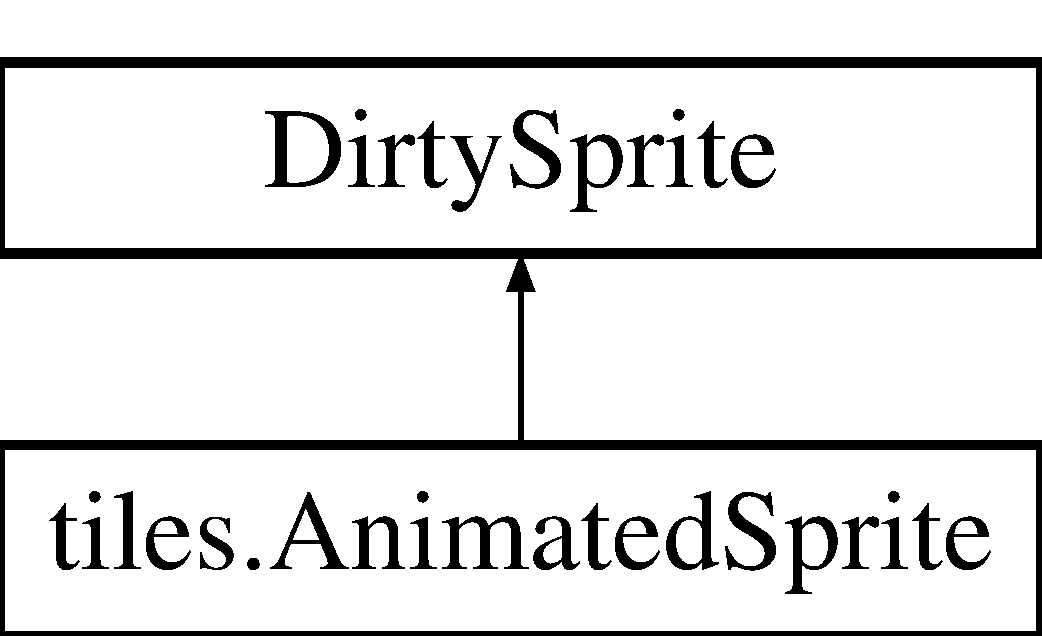
\includegraphics[height=2.000000cm]{classtiles_1_1AnimatedSprite}
\end{center}
\end{figure}
\subsection*{Public Member Functions}
\begin{DoxyCompactItemize}
\item 
\hypertarget{classtiles_1_1AnimatedSprite_ad45bb8638c7d1ffd137af2c0cb21a86a}{def {\bfseries \-\_\-\-\_\-init\-\_\-\-\_\-}}\label{classtiles_1_1AnimatedSprite_ad45bb8638c7d1ffd137af2c0cb21a86a}

\item 
\hypertarget{classtiles_1_1AnimatedSprite_a9dc14e2635930ba51d977455c7024eb0}{def {\bfseries reset}}\label{classtiles_1_1AnimatedSprite_a9dc14e2635930ba51d977455c7024eb0}

\item 
\hypertarget{classtiles_1_1AnimatedSprite_ad86444bfea97a89ca781a60f6e18fa28}{def {\bfseries update}}\label{classtiles_1_1AnimatedSprite_ad86444bfea97a89ca781a60f6e18fa28}

\end{DoxyCompactItemize}
\subsection*{Data Fields}
\begin{DoxyCompactItemize}
\item 
\hypertarget{classtiles_1_1AnimatedSprite_a532824d1725cfad4915d90c0eb5ceff0}{{\bfseries images}}\label{classtiles_1_1AnimatedSprite_a532824d1725cfad4915d90c0eb5ceff0}

\item 
\hypertarget{classtiles_1_1AnimatedSprite_a406749ec32f3d5406834948b79126332}{{\bfseries pos}}\label{classtiles_1_1AnimatedSprite_a406749ec32f3d5406834948b79126332}

\item 
\hypertarget{classtiles_1_1AnimatedSprite_ae80c4f033f04b8d7e32b61687892ce8e}{{\bfseries image}}\label{classtiles_1_1AnimatedSprite_ae80c4f033f04b8d7e32b61687892ce8e}

\item 
\hypertarget{classtiles_1_1AnimatedSprite_a8fecf17b5f1209c90035ff657d34ffb9}{{\bfseries rect}}\label{classtiles_1_1AnimatedSprite_a8fecf17b5f1209c90035ff657d34ffb9}

\item 
\hypertarget{classtiles_1_1AnimatedSprite_ae3ffcfa7a7f73aad07204fefda10b75b}{{\bfseries interval}}\label{classtiles_1_1AnimatedSprite_ae3ffcfa7a7f73aad07204fefda10b75b}

\item 
\hypertarget{classtiles_1_1AnimatedSprite_ac7f688c68e2fea34d53ccb57b81cb69e}{{\bfseries count}}\label{classtiles_1_1AnimatedSprite_ac7f688c68e2fea34d53ccb57b81cb69e}

\item 
\hypertarget{classtiles_1_1AnimatedSprite_ad3e171f6a1ec19006c0824eee5cc1db0}{{\bfseries dirty}}\label{classtiles_1_1AnimatedSprite_ad3e171f6a1ec19006c0824eee5cc1db0}

\end{DoxyCompactItemize}


\subsection{Detailed Description}


Definition at line 22 of file tiles.\-py.



The documentation for this class was generated from the following file\-:\begin{DoxyCompactItemize}
\item 
/home/antipant/\-Protocol\-P\-\_\-\-Project/\-U\-I/tiles.\-py\end{DoxyCompactItemize}

\hypertarget{classBGPMessage}{\section{B\-G\-P\-Message Class Reference}
\label{classBGPMessage}\index{B\-G\-P\-Message@{B\-G\-P\-Message}}
}
\subsection*{Public Member Functions}
\begin{DoxyCompactItemize}
\item 
\hypertarget{classBGPMessage_adc6bbac9250b1d246111183f8322f25f}{{\bfseries B\-G\-P\-Message} (\hyperlink{classBGPMessage}{B\-G\-P\-Message} \&p\-\_\-\-Msg)}\label{classBGPMessage_adc6bbac9250b1d246111183f8322f25f}

\item 
\hyperlink{classBGPMessage}{B\-G\-P\-Message} \& \hyperlink{classBGPMessage_ac24ad07e2e991aa00aca3b60ed15b869}{operator=} (const \hyperlink{classBGPMessage}{B\-G\-P\-Message} \&p\-\_\-\-Msg)
\begin{DoxyCompactList}\small\item\em Overload of assign operator. \end{DoxyCompactList}\item 
bool \hyperlink{classBGPMessage_a0bb89ae6df629fd0718ddd08453c1b61}{operator==} (const \hyperlink{classBGPMessage}{B\-G\-P\-Message} \&p\-\_\-\-Msg) const 
\begin{DoxyCompactList}\small\item\em Overload of compare operator. \end{DoxyCompactList}\item 
\hypertarget{classBGPMessage_a36db34985c63befc284448f562bab316}{void {\bfseries clear\-Message} (void)}\label{classBGPMessage_a36db34985c63befc284448f562bab316}

\end{DoxyCompactItemize}
\subsection*{Data Fields}
\begin{DoxyCompactItemize}
\item 
\hypertarget{classBGPMessage_a9710a231150dd9d3dffde8dabce92fb8}{int \hyperlink{classBGPMessage_a9710a231150dd9d3dffde8dabce92fb8}{m\-\_\-\-Type}}\label{classBGPMessage_a9710a231150dd9d3dffde8dabce92fb8}

\begin{DoxyCompactList}\small\item\em Holds the B\-G\-P message type value. \end{DoxyCompactList}\item 
\hypertarget{classBGPMessage_a4771242e2f77745ed88421240817d85f}{string \hyperlink{classBGPMessage_a4771242e2f77745ed88421240817d85f}{m\-\_\-\-B\-G\-P\-Identifier}}\label{classBGPMessage_a4771242e2f77745ed88421240817d85f}

\begin{DoxyCompactList}\small\item\em The originator's B\-G\-P identifier. \end{DoxyCompactList}\item 
\hypertarget{classBGPMessage_aa6d0e6ed2b166f769d57c255c0cb551a}{int \hyperlink{classBGPMessage_aa6d0e6ed2b166f769d57c255c0cb551a}{m\-\_\-\-Outbound\-Interface}}\label{classBGPMessage_aa6d0e6ed2b166f769d57c255c0cb551a}

\begin{DoxyCompactList}\small\item\em The originator's B\-G\-P identifier. \end{DoxyCompactList}\item 
\hypertarget{classBGPMessage_aaaa12a50a5b5a53bb7235a3f8462d8b1}{int \hyperlink{classBGPMessage_aaaa12a50a5b5a53bb7235a3f8462d8b1}{m\-\_\-\-A\-S}}\label{classBGPMessage_aaaa12a50a5b5a53bb7235a3f8462d8b1}

\begin{DoxyCompactList}\small\item\em A\-S identifier. \end{DoxyCompactList}\item 
\hypertarget{classBGPMessage_aa0928ff15ae83782dc580717bd9e1d8d}{int {\bfseries m\-\_\-\-Hold\-Down\-Time}}\label{classBGPMessage_aa0928ff15ae83782dc580717bd9e1d8d}

\item 
\hypertarget{classBGPMessage_ab556609df97434b77390af0ec1b582ea}{unsigned long {\bfseries m\-\_\-\-Msg\-Id}}\label{classBGPMessage_ab556609df97434b77390af0ec1b582ea}

\item 
\hypertarget{classBGPMessage_ae608943915516251f617ee85b232d979}{string \hyperlink{classBGPMessage_ae608943915516251f617ee85b232d979}{m\-\_\-\-Message}}\label{classBGPMessage_ae608943915516251f617ee85b232d979}

\begin{DoxyCompactList}\small\item\em B\-G\-P message fields. \end{DoxyCompactList}\end{DoxyCompactItemize}
\subsection*{Related Functions}
(Note that these are not member functions.) \begin{DoxyCompactItemize}
\item 
ostream \& \hyperlink{classBGPMessage_ace73025b1f5f8e0b2ea9be4f48da7cd7}{operator$<$$<$} (ostream \&os, \hyperlink{classBGPMessage}{B\-G\-P\-Message} const \&p\-\_\-\-Msg)
\begin{DoxyCompactList}\small\item\em Overload stream operator. \end{DoxyCompactList}\item 
void \hyperlink{classBGPMessage_a2c02e57efce9755d0f691fc39e0cde40}{sc\-\_\-trace} (sc\-\_\-trace\-\_\-file $\ast$p\-\_\-\-Trace\-File\-Pointer, const \hyperlink{classBGPMessage}{B\-G\-P\-Message} \&p\-\_\-\-Msg, const string \&p\-\_\-\-Trace\-Object\-Name)
\begin{DoxyCompactList}\small\item\em Set trace file for this packet. \end{DoxyCompactList}\end{DoxyCompactItemize}


\subsection{Detailed Description}


Definition at line 71 of file B\-G\-P\-Message.\-hpp.



\subsection{Member Function Documentation}
\hypertarget{classBGPMessage_ac24ad07e2e991aa00aca3b60ed15b869}{\index{B\-G\-P\-Message@{B\-G\-P\-Message}!operator=@{operator=}}
\index{operator=@{operator=}!BGPMessage@{B\-G\-P\-Message}}
\subsubsection[{operator=}]{\setlength{\rightskip}{0pt plus 5cm}{\bf B\-G\-P\-Message} \& B\-G\-P\-Message\-::operator= (
\begin{DoxyParamCaption}
\item[{const {\bf B\-G\-P\-Message} \&}]{p\-\_\-\-Msg}
\end{DoxyParamCaption}
)}}\label{classBGPMessage_ac24ad07e2e991aa00aca3b60ed15b869}


Overload of assign operator. 

Copy the data fields of given B\-G\-P\-Message-\/object to the this. Return a reference to this. 
\begin{DoxyParams}[1]{Parameters}
\mbox{\tt in}  & {\em \hyperlink{classPacket}{Packet}} & p\-\_\-\-B\-G\-P\-Message Reference to a Packet-\/object, which member values is to be assigned to the member fields of this object accordingly \\
\hline
\end{DoxyParams}
\begin{DoxyReturn}{Returns}
{\bfseries } $<$\-Packet$>$ Reference to this object 
\end{DoxyReturn}


Definition at line 19 of file B\-G\-P\-Message.\-cpp.

\hypertarget{classBGPMessage_a0bb89ae6df629fd0718ddd08453c1b61}{\index{B\-G\-P\-Message@{B\-G\-P\-Message}!operator==@{operator==}}
\index{operator==@{operator==}!BGPMessage@{B\-G\-P\-Message}}
\subsubsection[{operator==}]{\setlength{\rightskip}{0pt plus 5cm}bool B\-G\-P\-Message\-::operator== (
\begin{DoxyParamCaption}
\item[{const {\bf B\-G\-P\-Message} \&}]{p\-\_\-\-Msg}
\end{DoxyParamCaption}
) const}}\label{classBGPMessage_a0bb89ae6df629fd0718ddd08453c1b61}


Overload of compare operator. 

Compare the data fields of this pkt-\/object to the onces in the given pkt-\/object. 
\begin{DoxyParams}[1]{Parameters}
\mbox{\tt in}  & {\em \hyperlink{classBGPMessage}{B\-G\-P\-Message}} & p\-\_\-\-Msg Reference to a B\-G\-P\-Message-\/object to be compared with this object \\
\hline
\end{DoxyParams}
\begin{DoxyReturn}{Returns}
{\bfseries } $<$bool$>$ true if the member fields of both objects match otherwise false. 
\end{DoxyReturn}


Definition at line 36 of file B\-G\-P\-Message.\-cpp.



\subsection{Friends And Related Function Documentation}
\hypertarget{classBGPMessage_ace73025b1f5f8e0b2ea9be4f48da7cd7}{\index{B\-G\-P\-Message@{B\-G\-P\-Message}!operator$<$$<$@{operator$<$$<$}}
\index{operator$<$$<$@{operator$<$$<$}!BGPMessage@{B\-G\-P\-Message}}
\subsubsection[{operator$<$$<$}]{\setlength{\rightskip}{0pt plus 5cm}ostream\& operator$<$$<$ (
\begin{DoxyParamCaption}
\item[{ostream \&}]{os, }
\item[{{\bf B\-G\-P\-Message} const \&}]{p\-\_\-\-Msg}
\end{DoxyParamCaption}
)\hspace{0.3cm}{\ttfamily [friend]}}}\label{classBGPMessage_ace73025b1f5f8e0b2ea9be4f48da7cd7}


Overload stream operator. 

Write data members into given output stream. 
\begin{DoxyParams}[1]{Parameters}
\mbox{\tt in}  & {\em os} & Reference to outputstream in which the member field values is to be written. \\
\hline
\mbox{\tt in}  & {\em p\-\_\-\-Msg} & Reference to B\-G\-P\-Message-\/object, which member fields is to be written into outputstream. \\
\hline
\end{DoxyParams}
\begin{DoxyReturn}{Returns}
{\bfseries } $<$ostream$>$ Reference to the outputstream containing the written values 
\end{DoxyReturn}


Definition at line 135 of file B\-G\-P\-Message.\-hpp.

\hypertarget{classBGPMessage_a2c02e57efce9755d0f691fc39e0cde40}{\index{B\-G\-P\-Message@{B\-G\-P\-Message}!sc\-\_\-trace@{sc\-\_\-trace}}
\index{sc\-\_\-trace@{sc\-\_\-trace}!BGPMessage@{B\-G\-P\-Message}}
\subsubsection[{sc\-\_\-trace}]{\setlength{\rightskip}{0pt plus 5cm}void sc\-\_\-trace (
\begin{DoxyParamCaption}
\item[{sc\-\_\-trace\-\_\-file $\ast$}]{p\-\_\-\-Trace\-File\-Pointer, }
\item[{const {\bf B\-G\-P\-Message} \&}]{p\-\_\-\-Msg, }
\item[{const string \&}]{p\-\_\-\-Trace\-Object\-Name}
\end{DoxyParamCaption}
)\hspace{0.3cm}{\ttfamily [friend]}}}\label{classBGPMessage_a2c02e57efce9755d0f691fc39e0cde40}


Set trace file for this packet. 

All the member fields shall be traced. Allow system\-C library to access the private members of this class by declaring the function as friend 
\begin{DoxyParams}[1]{Parameters}
\mbox{\tt out}  & {\em sc\-\_\-trace\-\_\-file} & p\-\_\-\-Trace\-File\-Pointer Pointer to sc\-\_\-trace\-\_\-file-\/object \\
\hline
\mbox{\tt in}  & {\em \hyperlink{classBGPMessage}{B\-G\-P\-Message}} & p\-\_\-\-Msg Reference to B\-G\-P\-Message-\/object to be traced \\
\hline
\mbox{\tt in}  & {\em string} & p\-\_\-\-Trace\-Object\-Name Name of the Packet-\/object \\
\hline
\end{DoxyParams}


Definition at line 151 of file B\-G\-P\-Message.\-hpp.



The documentation for this class was generated from the following files\-:\begin{DoxyCompactItemize}
\item 
/home/antipant/\-Protocol\-P\-\_\-\-Project/\hyperlink{BGPMessage_8hpp}{B\-G\-P\-Message.\-hpp}\item 
/home/antipant/\-Protocol\-P\-\_\-\-Project/\hyperlink{BGPMessage_8cpp}{B\-G\-P\-Message.\-cpp}\end{DoxyCompactItemize}

\hypertarget{classBGPSession}{\section{B\-G\-P\-Session Class Reference}
\label{classBGPSession}\index{B\-G\-P\-Session@{B\-G\-P\-Session}}
}


\hyperlink{classBGPSession}{B\-G\-P\-Session} module handles the Hold\-Down and Keepalive timers of the session and sends keepalive messages to the session peer.  




{\ttfamily \#include $<$B\-G\-P\-Session.\-hpp$>$}

Inheritance diagram for B\-G\-P\-Session\-:\begin{figure}[H]
\begin{center}
\leavevmode
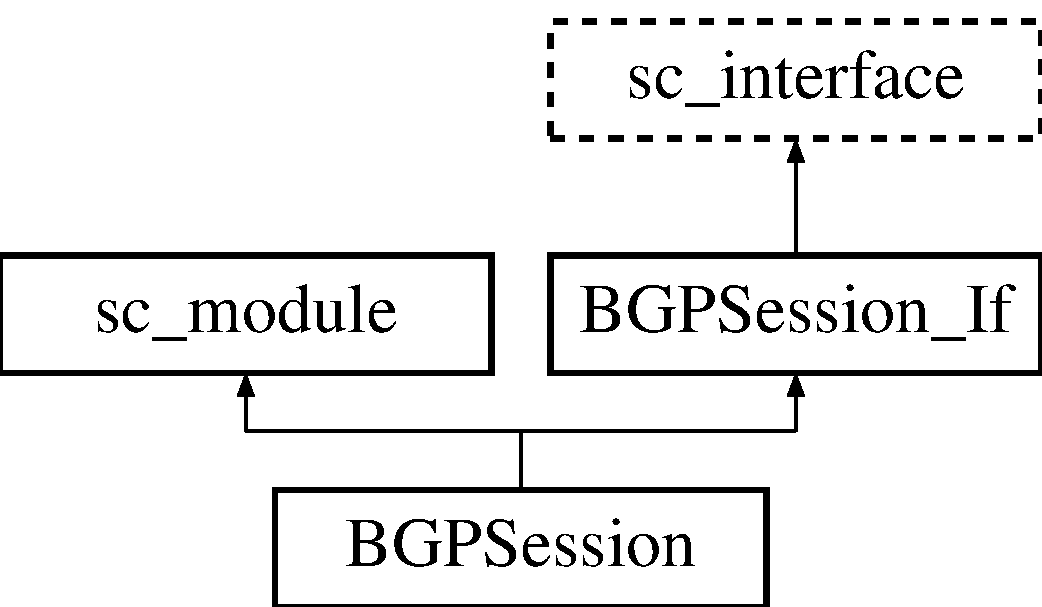
\includegraphics[height=3.000000cm]{classBGPSession}
\end{center}
\end{figure}
\subsection*{Public Member Functions}
\begin{DoxyCompactItemize}
\item 
\hypertarget{classBGPSession_ac518e0efd7d870a8ef4106ec32735b97}{void {\bfseries before\-\_\-end\-\_\-of\-\_\-elaboration} ()}\label{classBGPSession_ac518e0efd7d870a8ef4106ec32735b97}

\item 
\hyperlink{classBGPSession_a908e8994987c5d32129486f2fc265950}{B\-G\-P\-Session} (sc\-\_\-module\-\_\-name p\-\_\-\-Module\-Name, int p\-\_\-\-Peering\-Interface, \hyperlink{classBGPSessionParameters}{B\-G\-P\-Session\-Parameters} $\ast$const p\-\_\-\-Session\-Param)
\begin{DoxyCompactList}\small\item\em Elaborates the \hyperlink{classBGPSession}{B\-G\-P\-Session} module. \end{DoxyCompactList}\item 
\hyperlink{classBGPSession_a8c87d83d470539be218bb6903e5c10f3}{B\-G\-P\-Session} (sc\-\_\-module\-\_\-name p\-\_\-\-Module\-Name, \hyperlink{classBGPSessionParameters}{B\-G\-P\-Session\-Parameters} $\ast$const p\-\_\-\-Session\-Param)
\begin{DoxyCompactList}\small\item\em Elaborates the \hyperlink{classBGPSession}{B\-G\-P\-Session} module. \end{DoxyCompactList}\item 
\hyperlink{classBGPSession_aa948f6c710fb52d8a10a537c9ab67c08}{$\sim$\-B\-G\-P\-Session} ()
\begin{DoxyCompactList}\small\item\em Destructor of the \hyperlink{classBGPSession}{B\-G\-P\-Session} module. \end{DoxyCompactList}\item 
void \hyperlink{classBGPSession_a730132e1736499b9cf214bac62588b9d}{keepalive\-Timer} (void)
\begin{DoxyCompactList}\small\item\em Send a keepalive message to the peer. \end{DoxyCompactList}\item 
void \hyperlink{classBGPSession_ae996752db9e6063237d2d4bbd646f984}{session\-Invalidation} (void)
\begin{DoxyCompactList}\small\item\em Invalidates this session. \end{DoxyCompactList}\item 
void \hyperlink{classBGPSession_a895d45ac921090bcb8c87d95f2803e4b}{retransmission\-Timer} (void)
\begin{DoxyCompactList}\small\item\em Defines the retransmission period. \end{DoxyCompactList}\item 
\hypertarget{classBGPSession_aef60141c520d454fe87b50d070991212}{void \hyperlink{classBGPSession_aef60141c520d454fe87b50d070991212}{fsm\-Routine} (void)}\label{classBGPSession_aef60141c520d454fe87b50d070991212}

\begin{DoxyCompactList}\small\item\em Updates the session state. \end{DoxyCompactList}\item 
void \hyperlink{classBGPSession_a76d3bf3338ea7b3127999db4de73ec42}{reset\-Hold\-Down} (void)
\begin{DoxyCompactList}\small\item\em Resets the Hold\-Down timer. \end{DoxyCompactList}\item 
virtual bool \hyperlink{classBGPSession_a158bba46b42ee14afcac2bf53c68b309}{is\-Session\-Valid} (void)
\begin{DoxyCompactList}\small\item\em Checks whether this session is valid or not. \end{DoxyCompactList}\item 
virtual void \hyperlink{classBGPSession_a88e9285b17a692c2989923ad87b0587e}{session\-Stop} (void)
\begin{DoxyCompactList}\small\item\em Stops this session. \end{DoxyCompactList}\item 
void \hyperlink{classBGPSession_a1f47d3d32cc7c058bbefbad70a8596ea}{session\-Start} (void)
\begin{DoxyCompactList}\small\item\em Starts the session. \end{DoxyCompactList}\item 
void \hyperlink{classBGPSession_a41d56303c1f4fdfc6c51f869ac243998}{set\-Peer\-Identifier} (string p\-\_\-\-B\-G\-P\-Identifier)
\begin{DoxyCompactList}\small\item\em Sets the B\-G\-P Identifier of the session peer. \end{DoxyCompactList}\item 
void \hyperlink{classBGPSession_a7d3b4d6edbbf7bdfdd4150a10409564e}{set\-Peering\-Interface} (int p\-\_\-\-Interface)
\begin{DoxyCompactList}\small\item\em Set the interface id, which connects to the peering session. \end{DoxyCompactList}\item 
void \hyperlink{classBGPSession_af8838f841253356037b6d5e611f206ef}{set\-Peer\-A\-S} (int p\-\_\-\-Peer\-A\-S)
\item 
void \hyperlink{classBGPSession_acc7708be73adcedcbe269f2607d3184b}{set\-B\-G\-P\-Current\-State} (B\-G\-P\-\_\-\-States p\-\_\-\-State)
\begin{DoxyCompactList}\small\item\em Current F\-S\-M state of the B\-G\-P session. \end{DoxyCompactList}\item 
void \hyperlink{classBGPSession_a57a04a9247a8e5d04b393c6337958fb8}{set\-Connection\-Current\-State} (T\-C\-P\-\_\-\-States p\-\_\-\-State)
\begin{DoxyCompactList}\small\item\em Current F\-S\-M state of the T\-C\-P connection. \end{DoxyCompactList}\item 
void \hyperlink{classBGPSession_a70ec19b4e144f4785d7a3a9832c9b9ff}{set\-T\-C\-P\-Id} (int p\-\_\-\-Value)
\begin{DoxyCompactList}\small\item\em Holds the value of T\-C\-P id. \end{DoxyCompactList}\item 
bool \hyperlink{classBGPSession_a3ebc5dccec6c6655f24db4688869e17e}{is\-This\-Session} (string p\-\_\-\-B\-G\-P\-Identifier)
\begin{DoxyCompactList}\small\item\em Checks whether this session is for the passed B\-G\-P Identifier. \end{DoxyCompactList}\item 
\hypertarget{classBGPSession_ac6154f24eb86a2a724681f15cc66f793}{void \hyperlink{classBGPSession_ac6154f24eb86a2a724681f15cc66f793}{reset\-Keepalive} (void)}\label{classBGPSession_ac6154f24eb86a2a724681f15cc66f793}

\begin{DoxyCompactList}\small\item\em Resets the Keepalive timer. \end{DoxyCompactList}\item 
virtual int \hyperlink{classBGPSession_ad345c132ce5db5334b4c921fd745e642}{get\-Peering\-Interface} (void)
\item 
virtual string \hyperlink{classBGPSession_a663501b455c010d12e4cf1ff182e0355}{get\-Peer\-A\-S} (void)
\item 
virtual string \hyperlink{classBGPSession_ad74f8f645e0a99fcc115c3062985004f}{get\-Peer\-Identifier} (void)
\item 
B\-G\-P\-\_\-\-States \hyperlink{classBGPSession_a776c32ae58c02933a22ee23652d315da}{get\-B\-G\-P\-Current\-State} (void)
\begin{DoxyCompactList}\small\item\em Returns the current session state. \end{DoxyCompactList}\item 
T\-C\-P\-\_\-\-States \hyperlink{classBGPSession_ad636d249ffd53aa7a46bfcdf5091f9aa}{get\-Connection\-Current\-State} (void)
\begin{DoxyCompactList}\small\item\em Returns the current connection state. \end{DoxyCompactList}\item 
int \hyperlink{classBGPSession_a8110431fc392eff7efc7d5ab3a2a515d}{get\-T\-C\-P\-Id} (void)
\begin{DoxyCompactList}\small\item\em Returns the T\-C\-P I\-D. \end{DoxyCompactList}\item 
\hyperlink{classBGPSession_a112395018621c85ac62b43a2bcae211b}{S\-C\-\_\-\-H\-A\-S\-\_\-\-P\-R\-O\-C\-E\-S\-S} (\hyperlink{classBGPSession}{B\-G\-P\-Session})
\begin{DoxyCompactList}\small\item\em Indicate the system\-C producer that this module has a process. \end{DoxyCompactList}\end{DoxyCompactItemize}
\subsection*{Data Fields}
\begin{DoxyCompactItemize}
\item 
sc\-\_\-in\-\_\-clk \hyperlink{classBGPSession_adf7b7904c73267f2e6499ec4ffddee0e}{port\-\_\-\-Clk}
\begin{DoxyCompactList}\small\item\em System clock signal. \end{DoxyCompactList}\item 
sc\-\_\-port$<$ \hyperlink{classOutput__If}{Output\-\_\-\-If}$<$ \hyperlink{classBGPMessage}{B\-G\-P\-Message} $>$ $>$ \hyperlink{classBGPSession_ad7689f7d5de2710e4d9803de7e274517}{port\-\_\-\-To\-Data\-Plane}
\begin{DoxyCompactList}\small\item\em Output port to Data Plane module. \end{DoxyCompactList}\item 
\hypertarget{classBGPSession_a32b5d9138c0c9eb611e07f642b8397fc}{sc\-\_\-port$<$ \hyperlink{classOutput__If}{Output\-\_\-\-If}$<$ \hyperlink{classBGPMessage}{B\-G\-P\-Message} $>$ $>$ \hyperlink{classBGPSession_a32b5d9138c0c9eb611e07f642b8397fc}{port\-\_\-\-To\-Routing\-Table}}\label{classBGPSession_a32b5d9138c0c9eb611e07f642b8397fc}

\begin{DoxyCompactList}\small\item\em Output port to Routing \hyperlink{classTable}{Table} module. \end{DoxyCompactList}\item 
\hypertarget{classBGPSession_ac99274e961eb825ba3d4b61b52d242f4}{sc\-\_\-port$<$ \hyperlink{classInterface__If}{Interface\-\_\-\-If} $>$ \hyperlink{classBGPSession_ac99274e961eb825ba3d4b61b52d242f4}{port\-\_\-\-Interface\-Control}}\label{classBGPSession_ac99274e961eb825ba3d4b61b52d242f4}

\begin{DoxyCompactList}\small\item\em Control port to the session N\-I\-C. \end{DoxyCompactList}\item 
\hypertarget{classBGPSession_aac10fc66e70f5f0a42602b909f29adc9}{sc\-\_\-fifo$<$ \hyperlink{classBGPMessage}{B\-G\-P\-Message} $>$ {\bfseries m\-\_\-\-Fsm\-Input\-Buffer}}\label{classBGPSession_aac10fc66e70f5f0a42602b909f29adc9}

\end{DoxyCompactItemize}


\subsection{Detailed Description}
\hyperlink{classBGPSession}{B\-G\-P\-Session} module handles the Hold\-Down and Keepalive timers of the session and sends keepalive messages to the session peer. 

B\-G\-P session is a sub module of Control Plane. Control Plane has full control on B\-G\-P session. First the session is elaborated by Control Plane. Then the session is dedicated for some peer by assigning the peer's B\-G\-P identifier to the session. After that the session is started by calling the session\-Start-\/function. After that the session automatically send the keepalive messages to the peer whenever the keepalive timer expires. Control Plane needs to reset the Hold\-Down timer whenever it receives a message from the peer. Similarly, whenever Control Plane send a message to the peer, it shall reset the Keepalive timer of the session. The resets is done by calling the functions reset\-Hold\-Down and reset\-Keepalive. Control Plane can track message and the session by comparing the peer's identifier to the one in the session using the is\-This\-Session-\/function. When ever the Hold\-Down timer expires the session is stopped automatically. Control plane may check whether the session is still vaid or not using the is\-Session\-Valid-\/function. The checking shall be done before the timers are reset. Whenever Control Plane notices that the session is not valid it shall update the Routing table accordingly and generate required notification messages. 

Definition at line 67 of file B\-G\-P\-Session.\-hpp.



\subsection{Constructor \& Destructor Documentation}
\hypertarget{classBGPSession_a908e8994987c5d32129486f2fc265950}{\index{B\-G\-P\-Session@{B\-G\-P\-Session}!B\-G\-P\-Session@{B\-G\-P\-Session}}
\index{B\-G\-P\-Session@{B\-G\-P\-Session}!BGPSession@{B\-G\-P\-Session}}
\subsubsection[{B\-G\-P\-Session}]{\setlength{\rightskip}{0pt plus 5cm}B\-G\-P\-Session\-::\-B\-G\-P\-Session (
\begin{DoxyParamCaption}
\item[{sc\-\_\-module\-\_\-name}]{p\-\_\-\-Module\-Name, }
\item[{int}]{p\-\_\-\-Peering\-Interface, }
\item[{{\bf B\-G\-P\-Session\-Parameters} $\ast$const}]{p\-\_\-\-Session\-Param}
\end{DoxyParamCaption}
)}}\label{classBGPSession_a908e8994987c5d32129486f2fc265950}


Elaborates the \hyperlink{classBGPSession}{B\-G\-P\-Session} module. 


\begin{DoxyParams}[1]{Parameters}
\mbox{\tt in}  & {\em sc\-\_\-module\-\_\-name} & p\-\_\-\-Module\-Name Defines a unique name for this module \\
\hline
\mbox{\tt in}  & {\em int} & p\-\_\-\-Peering\-Interface The outbound interface to which the peer connects \\
\hline
\mbox{\tt in}  & {\em \hyperlink{classBGPSessionParameters}{B\-G\-P\-Session\-Parameters}} & p\-\_\-\-Session\-Parameters Holds the keepalive fraction, holddown time, etc. values for this session \\
\hline
\end{DoxyParams}


Definition at line 49 of file B\-G\-P\-Session.\-cpp.

\hypertarget{classBGPSession_a8c87d83d470539be218bb6903e5c10f3}{\index{B\-G\-P\-Session@{B\-G\-P\-Session}!B\-G\-P\-Session@{B\-G\-P\-Session}}
\index{B\-G\-P\-Session@{B\-G\-P\-Session}!BGPSession@{B\-G\-P\-Session}}
\subsubsection[{B\-G\-P\-Session}]{\setlength{\rightskip}{0pt plus 5cm}B\-G\-P\-Session\-::\-B\-G\-P\-Session (
\begin{DoxyParamCaption}
\item[{sc\-\_\-module\-\_\-name}]{p\-\_\-\-Module\-Name, }
\item[{{\bf B\-G\-P\-Session\-Parameters} $\ast$const}]{p\-\_\-\-Session\-Param}
\end{DoxyParamCaption}
)}}\label{classBGPSession_a8c87d83d470539be218bb6903e5c10f3}


Elaborates the \hyperlink{classBGPSession}{B\-G\-P\-Session} module. 


\begin{DoxyParams}[1]{Parameters}
\mbox{\tt in}  & {\em sc\-\_\-module\-\_\-name} & p\-\_\-\-Module\-Name Defines a unique name for this module \\
\hline
\mbox{\tt in}  & {\em \hyperlink{classBGPSessionParameters}{B\-G\-P\-Session\-Parameters}} & p\-\_\-\-Session\-Parameters Holds the keepalive fraction, holddown time, etc. values for this session \\
\hline
\end{DoxyParams}


Definition at line 13 of file B\-G\-P\-Session.\-cpp.

\hypertarget{classBGPSession_aa948f6c710fb52d8a10a537c9ab67c08}{\index{B\-G\-P\-Session@{B\-G\-P\-Session}!$\sim$\-B\-G\-P\-Session@{$\sim$\-B\-G\-P\-Session}}
\index{$\sim$\-B\-G\-P\-Session@{$\sim$\-B\-G\-P\-Session}!BGPSession@{B\-G\-P\-Session}}
\subsubsection[{$\sim$\-B\-G\-P\-Session}]{\setlength{\rightskip}{0pt plus 5cm}B\-G\-P\-Session\-::$\sim$\-B\-G\-P\-Session (
\begin{DoxyParamCaption}
{}
\end{DoxyParamCaption}
)}}\label{classBGPSession_aa948f6c710fb52d8a10a537c9ab67c08}


Destructor of the \hyperlink{classBGPSession}{B\-G\-P\-Session} module. 

Free's all the dynamically allocated memory 

Definition at line 92 of file B\-G\-P\-Session.\-cpp.



\subsection{Member Function Documentation}
\hypertarget{classBGPSession_a776c32ae58c02933a22ee23652d315da}{\index{B\-G\-P\-Session@{B\-G\-P\-Session}!get\-B\-G\-P\-Current\-State@{get\-B\-G\-P\-Current\-State}}
\index{get\-B\-G\-P\-Current\-State@{get\-B\-G\-P\-Current\-State}!BGPSession@{B\-G\-P\-Session}}
\subsubsection[{get\-B\-G\-P\-Current\-State}]{\setlength{\rightskip}{0pt plus 5cm}B\-G\-P\-\_\-\-States B\-G\-P\-Session\-::get\-B\-G\-P\-Current\-State (
\begin{DoxyParamCaption}
\item[{void}]{}
\end{DoxyParamCaption}
)}}\label{classBGPSession_a776c32ae58c02933a22ee23652d315da}


Returns the current session state. 

/fn B\-G\-P\-\_\-\-States \hyperlink{classBGPSession_a776c32ae58c02933a22ee23652d315da}{get\-B\-G\-P\-Current\-State(void)} 

Definition at line 556 of file B\-G\-P\-Session.\-cpp.

\hypertarget{classBGPSession_ad636d249ffd53aa7a46bfcdf5091f9aa}{\index{B\-G\-P\-Session@{B\-G\-P\-Session}!get\-Connection\-Current\-State@{get\-Connection\-Current\-State}}
\index{get\-Connection\-Current\-State@{get\-Connection\-Current\-State}!BGPSession@{B\-G\-P\-Session}}
\subsubsection[{get\-Connection\-Current\-State}]{\setlength{\rightskip}{0pt plus 5cm}T\-C\-P\-\_\-\-States B\-G\-P\-Session\-::get\-Connection\-Current\-State (
\begin{DoxyParamCaption}
\item[{void}]{}
\end{DoxyParamCaption}
)}}\label{classBGPSession_ad636d249ffd53aa7a46bfcdf5091f9aa}


Returns the current connection state. 

/fn T\-C\-P\-\_\-\-States \hyperlink{classBGPSession_ad636d249ffd53aa7a46bfcdf5091f9aa}{get\-Connection\-Current\-State(void)} 

Definition at line 561 of file B\-G\-P\-Session.\-cpp.

\hypertarget{classBGPSession_a663501b455c010d12e4cf1ff182e0355}{\index{B\-G\-P\-Session@{B\-G\-P\-Session}!get\-Peer\-A\-S@{get\-Peer\-A\-S}}
\index{get\-Peer\-A\-S@{get\-Peer\-A\-S}!BGPSession@{B\-G\-P\-Session}}
\subsubsection[{get\-Peer\-A\-S}]{\setlength{\rightskip}{0pt plus 5cm}string B\-G\-P\-Session\-::get\-Peer\-A\-S (
\begin{DoxyParamCaption}
\item[{void}]{}
\end{DoxyParamCaption}
)\hspace{0.3cm}{\ttfamily [virtual]}}}\label{classBGPSession_a663501b455c010d12e4cf1ff182e0355}
\begin{DoxySeeAlso}{See Also}
\hyperlink{classBGPSession__If}{B\-G\-P\-Session\-\_\-\-If}

\hyperlink{classBGPSession}{B\-G\-P\-Session} 
\end{DoxySeeAlso}


Implements \hyperlink{classBGPSession__If_a35753f07e12092da7c4270e45a8271a9}{B\-G\-P\-Session\-\_\-\-If}.



Definition at line 511 of file B\-G\-P\-Session.\-cpp.

\hypertarget{classBGPSession_ad74f8f645e0a99fcc115c3062985004f}{\index{B\-G\-P\-Session@{B\-G\-P\-Session}!get\-Peer\-Identifier@{get\-Peer\-Identifier}}
\index{get\-Peer\-Identifier@{get\-Peer\-Identifier}!BGPSession@{B\-G\-P\-Session}}
\subsubsection[{get\-Peer\-Identifier}]{\setlength{\rightskip}{0pt plus 5cm}string B\-G\-P\-Session\-::get\-Peer\-Identifier (
\begin{DoxyParamCaption}
\item[{void}]{}
\end{DoxyParamCaption}
)\hspace{0.3cm}{\ttfamily [virtual]}}}\label{classBGPSession_ad74f8f645e0a99fcc115c3062985004f}
\begin{DoxySeeAlso}{See Also}
\hyperlink{classBGPSession__If}{B\-G\-P\-Session\-\_\-\-If}

\hyperlink{classBGPSession}{B\-G\-P\-Session} 
\end{DoxySeeAlso}


Implements \hyperlink{classBGPSession__If_ad831c67d5d824798e18287e16da58967}{B\-G\-P\-Session\-\_\-\-If}.



Definition at line 549 of file B\-G\-P\-Session.\-cpp.

\hypertarget{classBGPSession_ad345c132ce5db5334b4c921fd745e642}{\index{B\-G\-P\-Session@{B\-G\-P\-Session}!get\-Peering\-Interface@{get\-Peering\-Interface}}
\index{get\-Peering\-Interface@{get\-Peering\-Interface}!BGPSession@{B\-G\-P\-Session}}
\subsubsection[{get\-Peering\-Interface}]{\setlength{\rightskip}{0pt plus 5cm}int B\-G\-P\-Session\-::get\-Peering\-Interface (
\begin{DoxyParamCaption}
\item[{void}]{}
\end{DoxyParamCaption}
)\hspace{0.3cm}{\ttfamily [virtual]}}}\label{classBGPSession_ad345c132ce5db5334b4c921fd745e642}
\begin{DoxySeeAlso}{See Also}
\hyperlink{classBGPSession__If}{B\-G\-P\-Session\-\_\-\-If}

\hyperlink{classBGPSession}{B\-G\-P\-Session} 
\end{DoxySeeAlso}


Implements \hyperlink{classBGPSession__If_aa280e6f0d7267d8fa6584913e54dd9ba}{B\-G\-P\-Session\-\_\-\-If}.



Definition at line 520 of file B\-G\-P\-Session.\-cpp.

\hypertarget{classBGPSession_a8110431fc392eff7efc7d5ab3a2a515d}{\index{B\-G\-P\-Session@{B\-G\-P\-Session}!get\-T\-C\-P\-Id@{get\-T\-C\-P\-Id}}
\index{get\-T\-C\-P\-Id@{get\-T\-C\-P\-Id}!BGPSession@{B\-G\-P\-Session}}
\subsubsection[{get\-T\-C\-P\-Id}]{\setlength{\rightskip}{0pt plus 5cm}int B\-G\-P\-Session\-::get\-T\-C\-P\-Id (
\begin{DoxyParamCaption}
\item[{void}]{}
\end{DoxyParamCaption}
)}}\label{classBGPSession_a8110431fc392eff7efc7d5ab3a2a515d}


Returns the T\-C\-P I\-D. 

/fn int \hyperlink{classBGPSession_a8110431fc392eff7efc7d5ab3a2a515d}{get\-T\-C\-P\-Id(void)} 

Definition at line 566 of file B\-G\-P\-Session.\-cpp.

\hypertarget{classBGPSession_a158bba46b42ee14afcac2bf53c68b309}{\index{B\-G\-P\-Session@{B\-G\-P\-Session}!is\-Session\-Valid@{is\-Session\-Valid}}
\index{is\-Session\-Valid@{is\-Session\-Valid}!BGPSession@{B\-G\-P\-Session}}
\subsubsection[{is\-Session\-Valid}]{\setlength{\rightskip}{0pt plus 5cm}bool B\-G\-P\-Session\-::is\-Session\-Valid (
\begin{DoxyParamCaption}
\item[{void}]{}
\end{DoxyParamCaption}
)\hspace{0.3cm}{\ttfamily [virtual]}}}\label{classBGPSession_a158bba46b42ee14afcac2bf53c68b309}


Checks whether this session is valid or not. 

Allows the control plane to check whether this session is still valid or not. I.\-e. is the Hold\-Down timer expired. 

Implements \hyperlink{classBGPSession__If_a774c827a52f62d49903daa2781769734}{B\-G\-P\-Session\-\_\-\-If}.



Definition at line 475 of file B\-G\-P\-Session.\-cpp.

\hypertarget{classBGPSession_a3ebc5dccec6c6655f24db4688869e17e}{\index{B\-G\-P\-Session@{B\-G\-P\-Session}!is\-This\-Session@{is\-This\-Session}}
\index{is\-This\-Session@{is\-This\-Session}!BGPSession@{B\-G\-P\-Session}}
\subsubsection[{is\-This\-Session}]{\setlength{\rightskip}{0pt plus 5cm}bool B\-G\-P\-Session\-::is\-This\-Session (
\begin{DoxyParamCaption}
\item[{string}]{p\-\_\-\-B\-G\-P\-Identifier}
\end{DoxyParamCaption}
)}}\label{classBGPSession_a3ebc5dccec6c6655f24db4688869e17e}


Checks whether this session is for the passed B\-G\-P Identifier. 


\begin{DoxyParams}[1]{Parameters}
\mbox{\tt in}  & {\em string} & p\-\_\-\-B\-G\-P\-Identifier The B\-G\-P Identifier of the received message \\
\hline
\end{DoxyParams}
\begin{DoxyReturn}{Returns}
$<$bool$>$ True\-: if this session corresponds the received message a identifier. False\-: in any other case 
\end{DoxyReturn}


Definition at line 480 of file B\-G\-P\-Session.\-cpp.

\hypertarget{classBGPSession_a730132e1736499b9cf214bac62588b9d}{\index{B\-G\-P\-Session@{B\-G\-P\-Session}!keepalive\-Timer@{keepalive\-Timer}}
\index{keepalive\-Timer@{keepalive\-Timer}!BGPSession@{B\-G\-P\-Session}}
\subsubsection[{keepalive\-Timer}]{\setlength{\rightskip}{0pt plus 5cm}void B\-G\-P\-Session\-::keepalive\-Timer (
\begin{DoxyParamCaption}
\item[{void}]{}
\end{DoxyParamCaption}
)}}\label{classBGPSession_a730132e1736499b9cf214bac62588b9d}


Send a keepalive message to the peer. 

A System\-C method, which is sensitive to m\-\_\-\-B\-G\-P\-Keepalive event 

Definition at line 99 of file B\-G\-P\-Session.\-cpp.

\hypertarget{classBGPSession_a76d3bf3338ea7b3127999db4de73ec42}{\index{B\-G\-P\-Session@{B\-G\-P\-Session}!reset\-Hold\-Down@{reset\-Hold\-Down}}
\index{reset\-Hold\-Down@{reset\-Hold\-Down}!BGPSession@{B\-G\-P\-Session}}
\subsubsection[{reset\-Hold\-Down}]{\setlength{\rightskip}{0pt plus 5cm}void B\-G\-P\-Session\-::reset\-Hold\-Down (
\begin{DoxyParamCaption}
\item[{void}]{}
\end{DoxyParamCaption}
)}}\label{classBGPSession_a76d3bf3338ea7b3127999db4de73ec42}


Resets the Hold\-Down timer. 

Allows the control plane to reset the Hold\-Down timer whenever a message from the session peer is received 

Definition at line 467 of file B\-G\-P\-Session.\-cpp.

\hypertarget{classBGPSession_a895d45ac921090bcb8c87d95f2803e4b}{\index{B\-G\-P\-Session@{B\-G\-P\-Session}!retransmission\-Timer@{retransmission\-Timer}}
\index{retransmission\-Timer@{retransmission\-Timer}!BGPSession@{B\-G\-P\-Session}}
\subsubsection[{retransmission\-Timer}]{\setlength{\rightskip}{0pt plus 5cm}void B\-G\-P\-Session\-::retransmission\-Timer (
\begin{DoxyParamCaption}
\item[{void}]{}
\end{DoxyParamCaption}
)}}\label{classBGPSession_a895d45ac921090bcb8c87d95f2803e4b}


Defines the retransmission period. 

The period length is set with m\-\_\-\-Retransmission event 

Definition at line 145 of file B\-G\-P\-Session.\-cpp.

\hypertarget{classBGPSession_a112395018621c85ac62b43a2bcae211b}{\index{B\-G\-P\-Session@{B\-G\-P\-Session}!S\-C\-\_\-\-H\-A\-S\-\_\-\-P\-R\-O\-C\-E\-S\-S@{S\-C\-\_\-\-H\-A\-S\-\_\-\-P\-R\-O\-C\-E\-S\-S}}
\index{S\-C\-\_\-\-H\-A\-S\-\_\-\-P\-R\-O\-C\-E\-S\-S@{S\-C\-\_\-\-H\-A\-S\-\_\-\-P\-R\-O\-C\-E\-S\-S}!BGPSession@{B\-G\-P\-Session}}
\subsubsection[{S\-C\-\_\-\-H\-A\-S\-\_\-\-P\-R\-O\-C\-E\-S\-S}]{\setlength{\rightskip}{0pt plus 5cm}B\-G\-P\-Session\-::\-S\-C\-\_\-\-H\-A\-S\-\_\-\-P\-R\-O\-C\-E\-S\-S (
\begin{DoxyParamCaption}
\item[{{\bf B\-G\-P\-Session}}]{}
\end{DoxyParamCaption}
)}}\label{classBGPSession_a112395018621c85ac62b43a2bcae211b}


Indicate the system\-C producer that this module has a process. 

\begin{DoxySeeAlso}{See Also}
\href{http://www.iro.umontreal.ca/~lablasso/docs/SystemC2.0.1/html/classproducer.html}{\tt http\-://www.\-iro.\-umontreal.\-ca/$\sim$lablasso/docs/\-System\-C2.\-0.\-1/html/classproducer.\-html} 
\end{DoxySeeAlso}
\hypertarget{classBGPSession_ae996752db9e6063237d2d4bbd646f984}{\index{B\-G\-P\-Session@{B\-G\-P\-Session}!session\-Invalidation@{session\-Invalidation}}
\index{session\-Invalidation@{session\-Invalidation}!BGPSession@{B\-G\-P\-Session}}
\subsubsection[{session\-Invalidation}]{\setlength{\rightskip}{0pt plus 5cm}void B\-G\-P\-Session\-::session\-Invalidation (
\begin{DoxyParamCaption}
\item[{void}]{}
\end{DoxyParamCaption}
)}}\label{classBGPSession_ae996752db9e6063237d2d4bbd646f984}


Invalidates this session. 

A System\-C method, which is sensitive to m\-\_\-\-B\-G\-P\-Hold\-Down event 

Definition at line 131 of file B\-G\-P\-Session.\-cpp.

\hypertarget{classBGPSession_a1f47d3d32cc7c058bbefbad70a8596ea}{\index{B\-G\-P\-Session@{B\-G\-P\-Session}!session\-Start@{session\-Start}}
\index{session\-Start@{session\-Start}!BGPSession@{B\-G\-P\-Session}}
\subsubsection[{session\-Start}]{\setlength{\rightskip}{0pt plus 5cm}void B\-G\-P\-Session\-::session\-Start (
\begin{DoxyParamCaption}
\item[{void}]{}
\end{DoxyParamCaption}
)}}\label{classBGPSession_a1f47d3d32cc7c058bbefbad70a8596ea}


Starts the session. 

Hold\-Down and Keepalive timers are reset and the sending of keepalive messages starts 

Definition at line 448 of file B\-G\-P\-Session.\-cpp.

\hypertarget{classBGPSession_a88e9285b17a692c2989923ad87b0587e}{\index{B\-G\-P\-Session@{B\-G\-P\-Session}!session\-Stop@{session\-Stop}}
\index{session\-Stop@{session\-Stop}!BGPSession@{B\-G\-P\-Session}}
\subsubsection[{session\-Stop}]{\setlength{\rightskip}{0pt plus 5cm}void B\-G\-P\-Session\-::session\-Stop (
\begin{DoxyParamCaption}
\item[{void}]{}
\end{DoxyParamCaption}
)\hspace{0.3cm}{\ttfamily [virtual]}}}\label{classBGPSession_a88e9285b17a692c2989923ad87b0587e}


Stops this session. 

Hold\-Down and Keepalive timers are stopped and no keepalive messages are sent after a call of this function 

Implements \hyperlink{classBGPSession__If_a9ba5b4e758982febdc4f71e01aae2b24}{B\-G\-P\-Session\-\_\-\-If}.



Definition at line 438 of file B\-G\-P\-Session.\-cpp.

\hypertarget{classBGPSession_acc7708be73adcedcbe269f2607d3184b}{\index{B\-G\-P\-Session@{B\-G\-P\-Session}!set\-B\-G\-P\-Current\-State@{set\-B\-G\-P\-Current\-State}}
\index{set\-B\-G\-P\-Current\-State@{set\-B\-G\-P\-Current\-State}!BGPSession@{B\-G\-P\-Session}}
\subsubsection[{set\-B\-G\-P\-Current\-State}]{\setlength{\rightskip}{0pt plus 5cm}void B\-G\-P\-Session\-::set\-B\-G\-P\-Current\-State (
\begin{DoxyParamCaption}
\item[{B\-G\-P\-\_\-\-States}]{p\-\_\-\-State}
\end{DoxyParamCaption}
)}}\label{classBGPSession_acc7708be73adcedcbe269f2607d3184b}


Current F\-S\-M state of the B\-G\-P session. 


\begin{DoxyParams}[1]{Parameters}
\mbox{\tt in}  & {\em B\-G\-P\-\_\-\-State} & p\-\_\-\-State \\
\hline
\end{DoxyParams}


Definition at line 492 of file B\-G\-P\-Session.\-cpp.

\hypertarget{classBGPSession_a57a04a9247a8e5d04b393c6337958fb8}{\index{B\-G\-P\-Session@{B\-G\-P\-Session}!set\-Connection\-Current\-State@{set\-Connection\-Current\-State}}
\index{set\-Connection\-Current\-State@{set\-Connection\-Current\-State}!BGPSession@{B\-G\-P\-Session}}
\subsubsection[{set\-Connection\-Current\-State}]{\setlength{\rightskip}{0pt plus 5cm}void B\-G\-P\-Session\-::set\-Connection\-Current\-State (
\begin{DoxyParamCaption}
\item[{T\-C\-P\-\_\-\-States}]{p\-\_\-\-State}
\end{DoxyParamCaption}
)}}\label{classBGPSession_a57a04a9247a8e5d04b393c6337958fb8}


Current F\-S\-M state of the T\-C\-P connection. 


\begin{DoxyParams}[1]{Parameters}
\mbox{\tt in}  & {\em T\-C\-P\-\_\-\-States} & p\-\_\-\-State \\
\hline
\end{DoxyParams}


Definition at line 499 of file B\-G\-P\-Session.\-cpp.

\hypertarget{classBGPSession_af8838f841253356037b6d5e611f206ef}{\index{B\-G\-P\-Session@{B\-G\-P\-Session}!set\-Peer\-A\-S@{set\-Peer\-A\-S}}
\index{set\-Peer\-A\-S@{set\-Peer\-A\-S}!BGPSession@{B\-G\-P\-Session}}
\subsubsection[{set\-Peer\-A\-S}]{\setlength{\rightskip}{0pt plus 5cm}void B\-G\-P\-Session\-::set\-Peer\-A\-S (
\begin{DoxyParamCaption}
\item[{int}]{p\-\_\-\-Peer\-A\-S}
\end{DoxyParamCaption}
)}}\label{classBGPSession_af8838f841253356037b6d5e611f206ef}
\begin{DoxySeeAlso}{See Also}
\hyperlink{classBGPSession}{B\-G\-P\-Session} 
\end{DoxySeeAlso}


Definition at line 537 of file B\-G\-P\-Session.\-cpp.

\hypertarget{classBGPSession_a41d56303c1f4fdfc6c51f869ac243998}{\index{B\-G\-P\-Session@{B\-G\-P\-Session}!set\-Peer\-Identifier@{set\-Peer\-Identifier}}
\index{set\-Peer\-Identifier@{set\-Peer\-Identifier}!BGPSession@{B\-G\-P\-Session}}
\subsubsection[{set\-Peer\-Identifier}]{\setlength{\rightskip}{0pt plus 5cm}void B\-G\-P\-Session\-::set\-Peer\-Identifier (
\begin{DoxyParamCaption}
\item[{string}]{p\-\_\-\-B\-G\-P\-Identifier}
\end{DoxyParamCaption}
)}}\label{classBGPSession_a41d56303c1f4fdfc6c51f869ac243998}


Sets the B\-G\-P Identifier of the session peer. 


\begin{DoxyParams}[1]{Parameters}
\mbox{\tt in}  & {\em string} & p\-\_\-\-B\-G\-P\-Identifier of the session peer received message \\
\hline
\end{DoxyParams}


Definition at line 487 of file B\-G\-P\-Session.\-cpp.

\hypertarget{classBGPSession_a7d3b4d6edbbf7bdfdd4150a10409564e}{\index{B\-G\-P\-Session@{B\-G\-P\-Session}!set\-Peering\-Interface@{set\-Peering\-Interface}}
\index{set\-Peering\-Interface@{set\-Peering\-Interface}!BGPSession@{B\-G\-P\-Session}}
\subsubsection[{set\-Peering\-Interface}]{\setlength{\rightskip}{0pt plus 5cm}void B\-G\-P\-Session\-::set\-Peering\-Interface (
\begin{DoxyParamCaption}
\item[{int}]{p\-\_\-\-Interface}
\end{DoxyParamCaption}
)}}\label{classBGPSession_a7d3b4d6edbbf7bdfdd4150a10409564e}


Set the interface id, which connects to the peering session. 

\begin{DoxySeeAlso}{See Also}
\hyperlink{classBGPSession}{B\-G\-P\-Session}
\end{DoxySeeAlso}

\begin{DoxyParams}[1]{Parameters}
\mbox{\tt in}  & {\em int} & p\-\_\-\-Interface \\
\hline
\end{DoxyParams}


Definition at line 527 of file B\-G\-P\-Session.\-cpp.

\hypertarget{classBGPSession_a70ec19b4e144f4785d7a3a9832c9b9ff}{\index{B\-G\-P\-Session@{B\-G\-P\-Session}!set\-T\-C\-P\-Id@{set\-T\-C\-P\-Id}}
\index{set\-T\-C\-P\-Id@{set\-T\-C\-P\-Id}!BGPSession@{B\-G\-P\-Session}}
\subsubsection[{set\-T\-C\-P\-Id}]{\setlength{\rightskip}{0pt plus 5cm}void B\-G\-P\-Session\-::set\-T\-C\-P\-Id (
\begin{DoxyParamCaption}
\item[{int}]{p\-\_\-\-Value}
\end{DoxyParamCaption}
)}}\label{classBGPSession_a70ec19b4e144f4785d7a3a9832c9b9ff}


Holds the value of T\-C\-P id. 


\begin{DoxyParams}[1]{Parameters}
\mbox{\tt in}  & {\em int} & p\-\_\-\-Value \\
\hline
\end{DoxyParams}


Definition at line 504 of file B\-G\-P\-Session.\-cpp.



\subsection{Field Documentation}
\hypertarget{classBGPSession_adf7b7904c73267f2e6499ec4ffddee0e}{\index{B\-G\-P\-Session@{B\-G\-P\-Session}!port\-\_\-\-Clk@{port\-\_\-\-Clk}}
\index{port\-\_\-\-Clk@{port\-\_\-\-Clk}!BGPSession@{B\-G\-P\-Session}}
\subsubsection[{port\-\_\-\-Clk}]{\setlength{\rightskip}{0pt plus 5cm}sc\-\_\-in\-\_\-clk B\-G\-P\-Session\-::port\-\_\-\-Clk}}\label{classBGPSession_adf7b7904c73267f2e6499ec4ffddee0e}


System clock signal. 

The router's internal clock 

Definition at line 76 of file B\-G\-P\-Session.\-hpp.

\hypertarget{classBGPSession_ad7689f7d5de2710e4d9803de7e274517}{\index{B\-G\-P\-Session@{B\-G\-P\-Session}!port\-\_\-\-To\-Data\-Plane@{port\-\_\-\-To\-Data\-Plane}}
\index{port\-\_\-\-To\-Data\-Plane@{port\-\_\-\-To\-Data\-Plane}!BGPSession@{B\-G\-P\-Session}}
\subsubsection[{port\-\_\-\-To\-Data\-Plane}]{\setlength{\rightskip}{0pt plus 5cm}sc\-\_\-port$<${\bf Output\-\_\-\-If}$<${\bf B\-G\-P\-Message}$>$ $>$ B\-G\-P\-Session\-::port\-\_\-\-To\-Data\-Plane}}\label{classBGPSession_ad7689f7d5de2710e4d9803de7e274517}


Output port to Data Plane module. 

The B\-G\-P session writes all the B\-G\-P messages to be send to its neighbors into this port. The port shall be bind to the Data Plane's. receiving F\-I\-F\-O 

Definition at line 85 of file B\-G\-P\-Session.\-hpp.



The documentation for this class was generated from the following files\-:\begin{DoxyCompactItemize}
\item 
/home/antipant/\-Protocol\-P\-\_\-\-Project/\hyperlink{BGPSession_8hpp}{B\-G\-P\-Session.\-hpp}\item 
/home/antipant/\-Protocol\-P\-\_\-\-Project/\hyperlink{BGPSession_8cpp}{B\-G\-P\-Session.\-cpp}\end{DoxyCompactItemize}

\hypertarget{classBGPSession__If}{\section{B\-G\-P\-Session\-\_\-\-If Class Reference}
\label{classBGPSession__If}\index{B\-G\-P\-Session\-\_\-\-If@{B\-G\-P\-Session\-\_\-\-If}}
}
Inheritance diagram for B\-G\-P\-Session\-\_\-\-If\-:\begin{figure}[H]
\begin{center}
\leavevmode
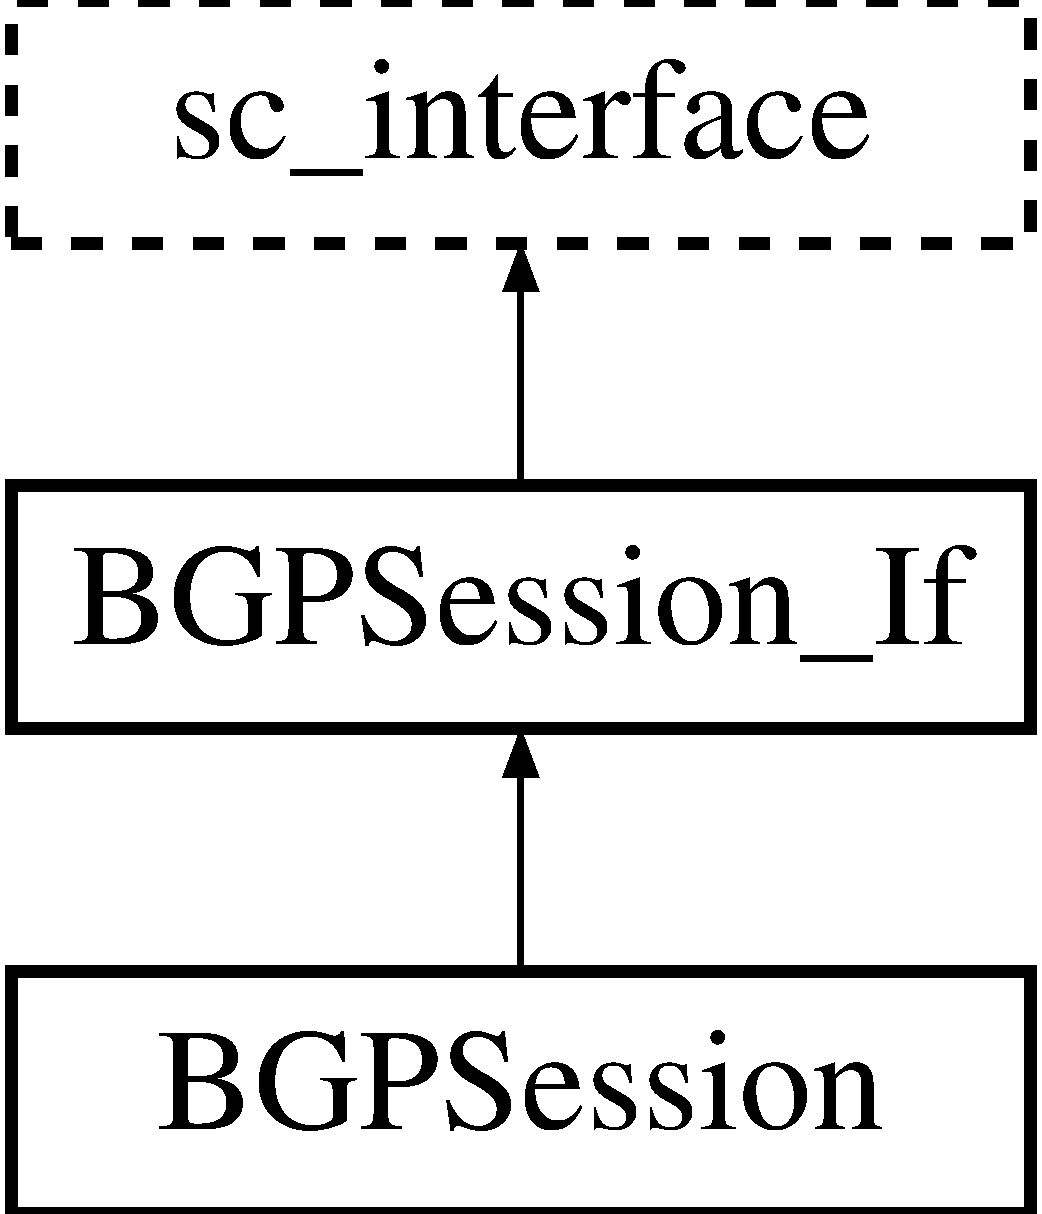
\includegraphics[height=3.000000cm]{classBGPSession__If}
\end{center}
\end{figure}
\subsection*{Public Member Functions}
\begin{DoxyCompactItemize}
\item 
virtual bool \hyperlink{classBGPSession__If_a774c827a52f62d49903daa2781769734}{is\-Session\-Valid} (void)=0
\begin{DoxyCompactList}\small\item\em Checks whether this session is valid or not. \end{DoxyCompactList}\item 
virtual void \hyperlink{classBGPSession__If_a9ba5b4e758982febdc4f71e01aae2b24}{session\-Stop} (void)=0
\begin{DoxyCompactList}\small\item\em Stops this session. \end{DoxyCompactList}\item 
virtual int \hyperlink{classBGPSession__If_aa280e6f0d7267d8fa6584913e54dd9ba}{get\-Peering\-Interface} (void)=0
\begin{DoxyCompactList}\small\item\em Returns the interface index of the session peer. \end{DoxyCompactList}\item 
virtual string \hyperlink{classBGPSession__If_a35753f07e12092da7c4270e45a8271a9}{get\-Peer\-A\-S} (void)=0
\begin{DoxyCompactList}\small\item\em Returns the A\-S number of the session peer. \end{DoxyCompactList}\item 
virtual string \hyperlink{classBGPSession__If_ad831c67d5d824798e18287e16da58967}{get\-Peer\-Identifier} (void)=0
\begin{DoxyCompactList}\small\item\em Return the Identifier of the session peer. \end{DoxyCompactList}\end{DoxyCompactItemize}


\subsection{Detailed Description}


Definition at line 29 of file B\-G\-P\-Session\-\_\-\-If.\-hpp.



\subsection{Member Function Documentation}
\hypertarget{classBGPSession__If_a35753f07e12092da7c4270e45a8271a9}{\index{B\-G\-P\-Session\-\_\-\-If@{B\-G\-P\-Session\-\_\-\-If}!get\-Peer\-A\-S@{get\-Peer\-A\-S}}
\index{get\-Peer\-A\-S@{get\-Peer\-A\-S}!BGPSession_If@{B\-G\-P\-Session\-\_\-\-If}}
\subsubsection[{get\-Peer\-A\-S}]{\setlength{\rightskip}{0pt plus 5cm}int virtual B\-G\-P\-Session\-\_\-\-If\-::get\-Peer\-A\-S (
\begin{DoxyParamCaption}
\item[{void}]{}
\end{DoxyParamCaption}
)\hspace{0.3cm}{\ttfamily [pure virtual]}}}\label{classBGPSession__If_a35753f07e12092da7c4270e45a8271a9}


Returns the A\-S number of the session peer. 

\begin{DoxyReturn}{Returns}
string\-: 
\end{DoxyReturn}


Implemented in \hyperlink{classBGPSession_a663501b455c010d12e4cf1ff182e0355}{B\-G\-P\-Session}.

\hypertarget{classBGPSession__If_ad831c67d5d824798e18287e16da58967}{\index{B\-G\-P\-Session\-\_\-\-If@{B\-G\-P\-Session\-\_\-\-If}!get\-Peer\-Identifier@{get\-Peer\-Identifier}}
\index{get\-Peer\-Identifier@{get\-Peer\-Identifier}!BGPSession_If@{B\-G\-P\-Session\-\_\-\-If}}
\subsubsection[{get\-Peer\-Identifier}]{\setlength{\rightskip}{0pt plus 5cm}string B\-G\-P\-Session\-\_\-\-If\-::get\-Peer\-Identifier (
\begin{DoxyParamCaption}
\item[{void}]{}
\end{DoxyParamCaption}
)\hspace{0.3cm}{\ttfamily [pure virtual]}}}\label{classBGPSession__If_ad831c67d5d824798e18287e16da58967}


Return the Identifier of the session peer. 

\begin{DoxyReturn}{Returns}
string\-: 
\end{DoxyReturn}


Implemented in \hyperlink{classBGPSession_ad74f8f645e0a99fcc115c3062985004f}{B\-G\-P\-Session}.

\hypertarget{classBGPSession__If_aa280e6f0d7267d8fa6584913e54dd9ba}{\index{B\-G\-P\-Session\-\_\-\-If@{B\-G\-P\-Session\-\_\-\-If}!get\-Peering\-Interface@{get\-Peering\-Interface}}
\index{get\-Peering\-Interface@{get\-Peering\-Interface}!BGPSession_If@{B\-G\-P\-Session\-\_\-\-If}}
\subsubsection[{get\-Peering\-Interface}]{\setlength{\rightskip}{0pt plus 5cm}int B\-G\-P\-Session\-\_\-\-If\-::get\-Peering\-Interface (
\begin{DoxyParamCaption}
\item[{void}]{}
\end{DoxyParamCaption}
)\hspace{0.3cm}{\ttfamily [pure virtual]}}}\label{classBGPSession__If_aa280e6f0d7267d8fa6584913e54dd9ba}


Returns the interface index of the session peer. 

\begin{DoxyReturn}{Returns}
int\-: 
\end{DoxyReturn}


Implemented in \hyperlink{classBGPSession_ad345c132ce5db5334b4c921fd745e642}{B\-G\-P\-Session}.

\hypertarget{classBGPSession__If_a774c827a52f62d49903daa2781769734}{\index{B\-G\-P\-Session\-\_\-\-If@{B\-G\-P\-Session\-\_\-\-If}!is\-Session\-Valid@{is\-Session\-Valid}}
\index{is\-Session\-Valid@{is\-Session\-Valid}!BGPSession_If@{B\-G\-P\-Session\-\_\-\-If}}
\subsubsection[{is\-Session\-Valid}]{\setlength{\rightskip}{0pt plus 5cm}bool B\-G\-P\-Session\-\_\-\-If\-::is\-Session\-Valid (
\begin{DoxyParamCaption}
\item[{void}]{}
\end{DoxyParamCaption}
)\hspace{0.3cm}{\ttfamily [pure virtual]}}}\label{classBGPSession__If_a774c827a52f62d49903daa2781769734}


Checks whether this session is valid or not. 

Allows the control plane to check whether this session is still valid or not. I.\-e. is the Hold\-Down timer expired. 

Implemented in \hyperlink{classBGPSession_a158bba46b42ee14afcac2bf53c68b309}{B\-G\-P\-Session}.

\hypertarget{classBGPSession__If_a9ba5b4e758982febdc4f71e01aae2b24}{\index{B\-G\-P\-Session\-\_\-\-If@{B\-G\-P\-Session\-\_\-\-If}!session\-Stop@{session\-Stop}}
\index{session\-Stop@{session\-Stop}!BGPSession_If@{B\-G\-P\-Session\-\_\-\-If}}
\subsubsection[{session\-Stop}]{\setlength{\rightskip}{0pt plus 5cm}void B\-G\-P\-Session\-\_\-\-If\-::session\-Stop (
\begin{DoxyParamCaption}
\item[{void}]{}
\end{DoxyParamCaption}
)\hspace{0.3cm}{\ttfamily [pure virtual]}}}\label{classBGPSession__If_a9ba5b4e758982febdc4f71e01aae2b24}


Stops this session. 

Hold\-Down and Keepalive timers are stopped and no keepalive messages are sent after a call of this function 

Implemented in \hyperlink{classBGPSession_a88e9285b17a692c2989923ad87b0587e}{B\-G\-P\-Session}.



The documentation for this class was generated from the following file\-:\begin{DoxyCompactItemize}
\item 
/home/antipant/\-Protocol\-P\-\_\-\-Project/\hyperlink{BGPSession__If_8hpp}{B\-G\-P\-Session\-\_\-\-If.\-hpp}\end{DoxyCompactItemize}

\hypertarget{classBGPSessionParameters}{\section{B\-G\-P\-Session\-Parameters Class Reference}
\label{classBGPSessionParameters}\index{B\-G\-P\-Session\-Parameters@{B\-G\-P\-Session\-Parameters}}
}


Holds the parameters for B\-G\-P session.  




{\ttfamily \#include $<$Configuration.\-hpp$>$}

Inheritance diagram for B\-G\-P\-Session\-Parameters\-:\begin{figure}[H]
\begin{center}
\leavevmode
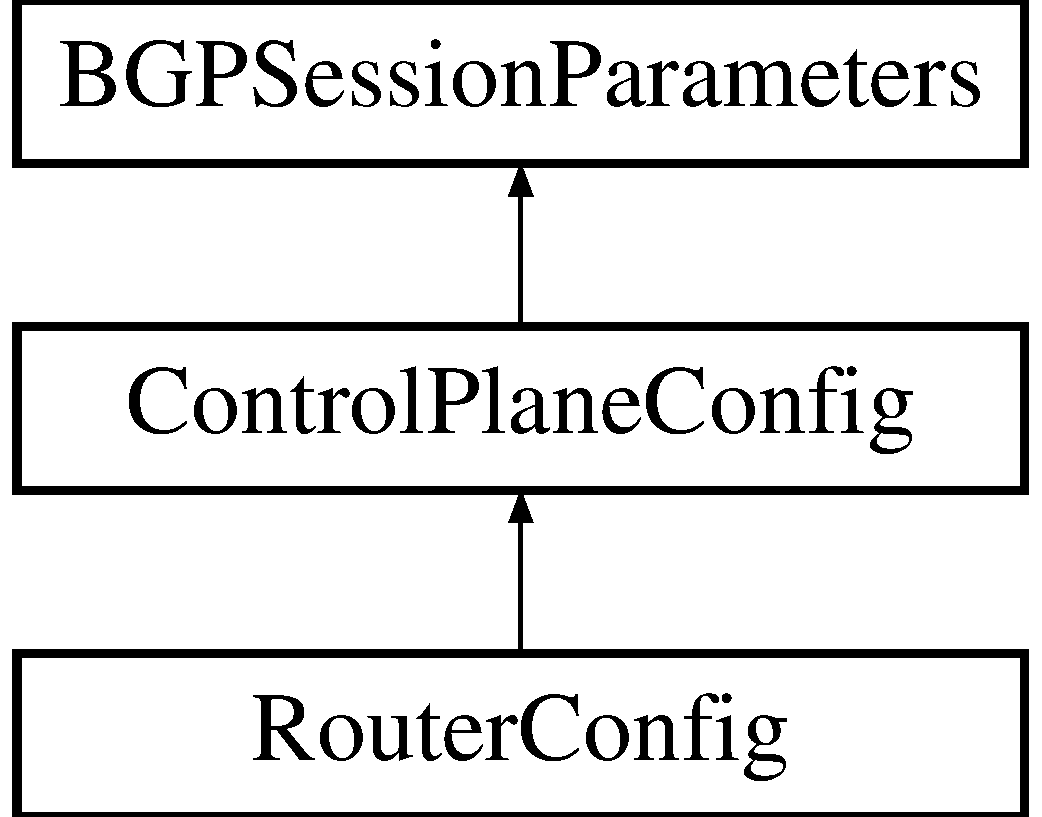
\includegraphics[height=3.000000cm]{classBGPSessionParameters}
\end{center}
\end{figure}
\subsection*{Public Member Functions}
\begin{DoxyCompactItemize}
\item 
\hyperlink{classBGPSessionParameters_ae3d4f579822be095d01bfd4cab18033e}{B\-G\-P\-Session\-Parameters} ()
\begin{DoxyCompactList}\small\item\em Implementation of Configuration classes. \end{DoxyCompactList}\item 
\hyperlink{classBGPSessionParameters_a11f44412906552a220daff73da0c1992}{B\-G\-P\-Session\-Parameters} (int p\-\_\-\-Keepalive\-Time, int p\-\_\-\-Hold\-Down\-Time\-Factor)
\item 
virtual \hyperlink{classBGPSessionParameters_a3f2dc608214dc93d33862c194be3fbee}{$\sim$\-B\-G\-P\-Session\-Parameters} ()
\item 
void \hyperlink{classBGPSessionParameters_af9feb193d7de00f2e44d9866dc7c7100}{set\-Keepalive\-Time} (int p\-\_\-\-Keepalive\-Time)
\begin{DoxyCompactList}\small\item\em Sets the Keepalive time. \end{DoxyCompactList}\item 
\hypertarget{classBGPSessionParameters_a4164a26b4457a22e93fd78f098c1691c}{void {\bfseries set\-Hold\-Down\-Time} (int p\-\_\-\-Hold\-Down\-Time)}\label{classBGPSessionParameters_a4164a26b4457a22e93fd78f098c1691c}

\item 
void \hyperlink{classBGPSessionParameters_a9ecde9c6514a451337b8f3043268286e}{set\-Hold\-Down\-Time\-Factor} (int p\-\_\-\-Hold\-Down\-Time\-Factor)
\begin{DoxyCompactList}\small\item\em Sets the Hold\-Down time factor. \end{DoxyCompactList}\item 
void \hyperlink{classBGPSessionParameters_a7348f562b2c3a6acec49cf2d10c535b1}{set\-N\-I\-C\-Mode} (int p\-\_\-\-Interface, int p\-\_\-\-Mode)
\begin{DoxyCompactList}\small\item\em Sets the interface mode used in T\-C\-P session establishment. \end{DoxyCompactList}\item 
\hypertarget{classBGPSessionParameters_abbb9bf5608aa7a47047496bf2a04d46e}{int {\bfseries get\-N\-I\-C\-Mode} (int p\-\_\-\-Interface)}\label{classBGPSessionParameters_abbb9bf5608aa7a47047496bf2a04d46e}

\item 
int \hyperlink{classBGPSessionParameters_ad1c71417fc4b9361f4ef49734c580418}{get\-Keepalive\-Time} (void)
\begin{DoxyCompactList}\small\item\em Returns the keepalive time. \end{DoxyCompactList}\item 
int \hyperlink{classBGPSessionParameters_ad38c18d312e65ab03f6bc3f4b659c4ce}{get\-Hold\-Down\-Time} (void)
\begin{DoxyCompactList}\small\item\em Returns the hold-\/down time. \end{DoxyCompactList}\item 
int \hyperlink{classBGPSessionParameters_a67b75e762c37bc79afe0c23d32ceec4f}{get\-Hol\-Down\-Time\-Factor} (void)
\begin{DoxyCompactList}\small\item\em Returns the hold-\/down time factor. \end{DoxyCompactList}\item 
bool \hyperlink{classBGPSessionParameters_a2681ec8adc40cc7dac2a03e7cb3d1994}{is\-Client} (int p\-\_\-\-Interface)
\begin{DoxyCompactList}\small\item\em Checks whether the given interface is in the client mode. \end{DoxyCompactList}\item 
void \hyperlink{classBGPSessionParameters_a7e04197d15b3df124836aad920ea2d1a}{set\-Prefix} (string p\-\_\-\-Prefix)
\begin{DoxyCompactList}\small\item\em Sets the prefix I\-P of the A\-S as string. \end{DoxyCompactList}\item 
void \hyperlink{classBGPSessionParameters_a943d68b6970da3a82b81d89b16fe3aeb}{set\-Prefix} (sc\-\_\-uint$<$ 32 $>$ p\-\_\-\-Prefix)
\begin{DoxyCompactList}\small\item\em Sets the prefix I\-P of the A\-S. \end{DoxyCompactList}\item 
void \hyperlink{classBGPSessionParameters_a2a7ad268d1b26c1de1cb6b793bc8a5db}{set\-Prefix\-Mask} (sc\-\_\-uint$<$ 32 $>$ p\-\_\-\-Prefix\-Mask)
\begin{DoxyCompactList}\small\item\em Sets the mask for the prefix I\-P. \end{DoxyCompactList}\item 
\hypertarget{classBGPSessionParameters_a46ce107efaa09ccdb5a226c9e52976e9}{void {\bfseries set\-A\-S\-Number} (int p\-\_\-\-A\-S\-Number)}\label{classBGPSessionParameters_a46ce107efaa09ccdb5a226c9e52976e9}

\item 
void \hyperlink{classBGPSessionParameters_ab6f1e71374d250392eabe4571245137d}{set\-M\-E\-D} (int p\-\_\-\-M\-E\-D)
\begin{DoxyCompactList}\small\item\em Sets the Multi-\/exit discriminator(\-M\-E\-D) attribute of B\-G\-P. \end{DoxyCompactList}\item 
void \hyperlink{classBGPSessionParameters_a898ff54a5ddb05b8212fe8b1cdbb16be}{set\-Local\-Pref} (int p\-\_\-\-Local\-Pref)
\begin{DoxyCompactList}\small\item\em Sets the Local Preference atribute of B\-G\-P. \end{DoxyCompactList}\item 
string \hyperlink{classBGPSessionParameters_a4221d963d60974d8236164b29743aec8}{get\-I\-P\-As\-String} (void)
\begin{DoxyCompactList}\small\item\em Returns the I\-P prefix as string. \end{DoxyCompactList}\item 
string \hyperlink{classBGPSessionParameters_a5da0c2ccd227626e379db649965ee5f2}{get\-B\-G\-P\-Identifier} (void)
\begin{DoxyCompactList}\small\item\em Returns the B\-G\-P identifier I\-P. \end{DoxyCompactList}\item 
string \hyperlink{classBGPSessionParameters_a5e810c8d0bd6eff56233507adf6dabe7}{get\-I\-P\-Mask\-As\-String} (void)
\begin{DoxyCompactList}\small\item\em Returns the prefix mask value\-: the number of bits set to one starting from the 31st bit. \end{DoxyCompactList}\item 
sc\-\_\-uint$<$ 32 $>$ \hyperlink{classBGPSessionParameters_a32780ac488ad12575334f9b004426bc3}{get\-Prefix} (void)
\begin{DoxyCompactList}\small\item\em Returns the I\-P prefix. \end{DoxyCompactList}\item 
sc\-\_\-uint$<$ 32 $>$ \hyperlink{classBGPSessionParameters_afa843363c1ad8881e957c5a7a53004a9}{get\-Prefix\-Mask} (void)
\begin{DoxyCompactList}\small\item\em Returns the prefix mask. \end{DoxyCompactList}\item 
int \hyperlink{classBGPSessionParameters_afc93bac9efde675d8071894ee95c021a}{get\-A\-S\-Number} (void)
\begin{DoxyCompactList}\small\item\em Returns the A\-S number. \end{DoxyCompactList}\item 
\hypertarget{classBGPSessionParameters_a740e52b61810ef405acc6ade93e796b4}{string {\bfseries get\-A\-S\-Number\-As\-String} (void)}\label{classBGPSessionParameters_a740e52b61810ef405acc6ade93e796b4}

\item 
int \hyperlink{classBGPSessionParameters_ab3f7cbe1af9f3ce6965042ea39250cb9}{get\-M\-E\-D} (void)
\begin{DoxyCompactList}\small\item\em Returns the Multi-\/exit discriminator value. \end{DoxyCompactList}\item 
int \hyperlink{classBGPSessionParameters_a4ee03778f9715e90243fc16a47514f64}{get\-Local\-Pref} (void)
\begin{DoxyCompactList}\small\item\em Returns the Local preference value. \end{DoxyCompactList}\item 
\hyperlink{classBGPSessionParameters}{B\-G\-P\-Session\-Parameters} \& \hyperlink{classBGPSessionParameters_aa15e1258ca1d21dabb6d146a38a051cb}{operator=} (const \hyperlink{classBGPSessionParameters}{B\-G\-P\-Session\-Parameters} \&p\-\_\-\-Original)
\begin{DoxyCompactList}\small\item\em clones the passed \hyperlink{classBGPSessionParameters}{B\-G\-P\-Session\-Parameters} object to this object \end{DoxyCompactList}\end{DoxyCompactItemize}
\subsection*{Data Fields}
\begin{DoxyCompactItemize}
\item 
\hypertarget{classBGPSessionParameters_aa7bb99315626377510fd16ba688a3ff4}{sc\-\_\-uint$<$ 32 $>$ \hyperlink{classBGPSessionParameters_aa7bb99315626377510fd16ba688a3ff4}{m\-\_\-\-Prefix\-Mask}}\label{classBGPSessionParameters_aa7bb99315626377510fd16ba688a3ff4}

\begin{DoxyCompactList}\small\item\em The mask defined by prefix /-\/notation. \end{DoxyCompactList}\end{DoxyCompactItemize}
\subsection*{Protected Attributes}
\begin{DoxyCompactItemize}
\item 
int \hyperlink{classBGPSessionParameters_a465c4710f73834f9d0daaf9defe6ccc8}{m\-\_\-\-Keepalive\-Time}
\begin{DoxyCompactList}\small\item\em Hold\-Down time for this session. \end{DoxyCompactList}\item 
int \hyperlink{classBGPSessionParameters_aadc4f5c38dc8e8d4765391aaad8b5c5c}{m\-\_\-\-Hold\-Down\-Time}
\begin{DoxyCompactList}\small\item\em Hold\-Down time for this session. \end{DoxyCompactList}\item 
int \hyperlink{classBGPSessionParameters_a363e577b5765ea3c0bafa2b7a66efa7a}{m\-\_\-\-Hold\-Down\-Time\-Factor}
\begin{DoxyCompactList}\small\item\em Hold\-Down time factor. \end{DoxyCompactList}\item 
\hypertarget{classBGPSessionParameters_a817cad3f0d23762e4bfe5d0e38d82ea4}{int $\ast$ \hyperlink{classBGPSessionParameters_a817cad3f0d23762e4bfe5d0e38d82ea4}{m\-\_\-\-N\-I\-C\-Mode}}\label{classBGPSessionParameters_a817cad3f0d23762e4bfe5d0e38d82ea4}

\begin{DoxyCompactList}\small\item\em holds the network interface mode information \end{DoxyCompactList}\item 
\hypertarget{classBGPSessionParameters_a010fa1f90adcad91d8e1ba027b88860a}{sc\-\_\-uint$<$ 32 $>$ \hyperlink{classBGPSessionParameters_a010fa1f90adcad91d8e1ba027b88860a}{m\-\_\-\-Prefix}}\label{classBGPSessionParameters_a010fa1f90adcad91d8e1ba027b88860a}

\begin{DoxyCompactList}\small\item\em The prefix of the A\-S connecting this router. \end{DoxyCompactList}\item 
\hypertarget{classBGPSessionParameters_a9c063d3534b94fc0987f4942380a1657}{int \hyperlink{classBGPSessionParameters_a9c063d3534b94fc0987f4942380a1657}{m\-\_\-\-A\-S\-Number}}\label{classBGPSessionParameters_a9c063d3534b94fc0987f4942380a1657}

\begin{DoxyCompactList}\small\item\em The A\-S number of this router. \end{DoxyCompactList}\item 
\hypertarget{classBGPSessionParameters_ab6e0afde596352b6b1df9c207c67277a}{int \hyperlink{classBGPSessionParameters_ab6e0afde596352b6b1df9c207c67277a}{m\-\_\-\-M\-E\-D}}\label{classBGPSessionParameters_ab6e0afde596352b6b1df9c207c67277a}

\begin{DoxyCompactList}\small\item\em B\-G\-P M\-E\-D variable. \end{DoxyCompactList}\item 
\hypertarget{classBGPSessionParameters_a60219f0863cc5803a0c73dcdfc95d958}{int \hyperlink{classBGPSessionParameters_a60219f0863cc5803a0c73dcdfc95d958}{m\-\_\-\-Local\-Pref}}\label{classBGPSessionParameters_a60219f0863cc5803a0c73dcdfc95d958}

\begin{DoxyCompactList}\small\item\em B\-G\-P Local Preference variable. \end{DoxyCompactList}\end{DoxyCompactItemize}


\subsection{Detailed Description}
Holds the parameters for B\-G\-P session. 

Members are Keepalive time and Hold\-Down time factor 

Definition at line 28 of file Configuration.\-hpp.



\subsection{Constructor \& Destructor Documentation}
\hypertarget{classBGPSessionParameters_ae3d4f579822be095d01bfd4cab18033e}{\index{B\-G\-P\-Session\-Parameters@{B\-G\-P\-Session\-Parameters}!B\-G\-P\-Session\-Parameters@{B\-G\-P\-Session\-Parameters}}
\index{B\-G\-P\-Session\-Parameters@{B\-G\-P\-Session\-Parameters}!BGPSessionParameters@{B\-G\-P\-Session\-Parameters}}
\subsubsection[{B\-G\-P\-Session\-Parameters}]{\setlength{\rightskip}{0pt plus 5cm}B\-G\-P\-Session\-Parameters\-::\-B\-G\-P\-Session\-Parameters (
\begin{DoxyParamCaption}
{}
\end{DoxyParamCaption}
)}}\label{classBGPSessionParameters_ae3d4f579822be095d01bfd4cab18033e}


Implementation of Configuration classes. 

Default constructor of B\-G\-P\-Session\-Parameters-\/class

Sets the keepalive time to 60 and the holddown time factor to 3 

Definition at line 17 of file Configuration.\-cpp.

\hypertarget{classBGPSessionParameters_a11f44412906552a220daff73da0c1992}{\index{B\-G\-P\-Session\-Parameters@{B\-G\-P\-Session\-Parameters}!B\-G\-P\-Session\-Parameters@{B\-G\-P\-Session\-Parameters}}
\index{B\-G\-P\-Session\-Parameters@{B\-G\-P\-Session\-Parameters}!BGPSessionParameters@{B\-G\-P\-Session\-Parameters}}
\subsubsection[{B\-G\-P\-Session\-Parameters}]{\setlength{\rightskip}{0pt plus 5cm}B\-G\-P\-Session\-Parameters\-::\-B\-G\-P\-Session\-Parameters (
\begin{DoxyParamCaption}
\item[{int}]{p\-\_\-\-Keepalive\-Time, }
\item[{int}]{p\-\_\-\-Hold\-Down\-Time\-Factor}
\end{DoxyParamCaption}
)}}\label{classBGPSessionParameters_a11f44412906552a220daff73da0c1992}
Constructor of B\-G\-P\-Session\-Parameters-\/class with parameters

Allows to set the member values while initiating the object 
\begin{DoxyParams}[1]{Parameters}
\mbox{\tt in}  & {\em int} & p\-\_\-\-Keepalive\-Time The keepalive time value \\
\hline
\mbox{\tt in}  & {\em int} & p\-\_\-\-Hold\-Down\-Time\-Factor The multiplier that defines the Hold\-Down time in relation to Keepalive time. \\
\hline
\end{DoxyParams}


Definition at line 22 of file Configuration.\-cpp.

\hypertarget{classBGPSessionParameters_a3f2dc608214dc93d33862c194be3fbee}{\index{B\-G\-P\-Session\-Parameters@{B\-G\-P\-Session\-Parameters}!$\sim$\-B\-G\-P\-Session\-Parameters@{$\sim$\-B\-G\-P\-Session\-Parameters}}
\index{$\sim$\-B\-G\-P\-Session\-Parameters@{$\sim$\-B\-G\-P\-Session\-Parameters}!BGPSessionParameters@{B\-G\-P\-Session\-Parameters}}
\subsubsection[{$\sim$\-B\-G\-P\-Session\-Parameters}]{\setlength{\rightskip}{0pt plus 5cm}B\-G\-P\-Session\-Parameters\-::$\sim$\-B\-G\-P\-Session\-Parameters (
\begin{DoxyParamCaption}
{}
\end{DoxyParamCaption}
)\hspace{0.3cm}{\ttfamily [virtual]}}}\label{classBGPSessionParameters_a3f2dc608214dc93d33862c194be3fbee}
Default destructor

The class does not contain dynamic memory allocations 

Definition at line 27 of file Configuration.\-cpp.



\subsection{Member Function Documentation}
\hypertarget{classBGPSessionParameters_afc93bac9efde675d8071894ee95c021a}{\index{B\-G\-P\-Session\-Parameters@{B\-G\-P\-Session\-Parameters}!get\-A\-S\-Number@{get\-A\-S\-Number}}
\index{get\-A\-S\-Number@{get\-A\-S\-Number}!BGPSessionParameters@{B\-G\-P\-Session\-Parameters}}
\subsubsection[{get\-A\-S\-Number}]{\setlength{\rightskip}{0pt plus 5cm}int B\-G\-P\-Session\-Parameters\-::get\-A\-S\-Number (
\begin{DoxyParamCaption}
\item[{void}]{}
\end{DoxyParamCaption}
)}}\label{classBGPSessionParameters_afc93bac9efde675d8071894ee95c021a}


Returns the A\-S number. 

\begin{DoxyReturn}{Returns}
integer value 
\end{DoxyReturn}


Definition at line 142 of file Configuration.\-cpp.

\hypertarget{classBGPSessionParameters_a5da0c2ccd227626e379db649965ee5f2}{\index{B\-G\-P\-Session\-Parameters@{B\-G\-P\-Session\-Parameters}!get\-B\-G\-P\-Identifier@{get\-B\-G\-P\-Identifier}}
\index{get\-B\-G\-P\-Identifier@{get\-B\-G\-P\-Identifier}!BGPSessionParameters@{B\-G\-P\-Session\-Parameters}}
\subsubsection[{get\-B\-G\-P\-Identifier}]{\setlength{\rightskip}{0pt plus 5cm}string B\-G\-P\-Session\-Parameters\-::get\-B\-G\-P\-Identifier (
\begin{DoxyParamCaption}
\item[{void}]{}
\end{DoxyParamCaption}
)}}\label{classBGPSessionParameters_a5da0c2ccd227626e379db649965ee5f2}


Returns the B\-G\-P identifier I\-P. 

\begin{DoxyReturn}{Returns}
string value 
\end{DoxyReturn}


Definition at line 134 of file Configuration.\-cpp.

\hypertarget{classBGPSessionParameters_ad38c18d312e65ab03f6bc3f4b659c4ce}{\index{B\-G\-P\-Session\-Parameters@{B\-G\-P\-Session\-Parameters}!get\-Hold\-Down\-Time@{get\-Hold\-Down\-Time}}
\index{get\-Hold\-Down\-Time@{get\-Hold\-Down\-Time}!BGPSessionParameters@{B\-G\-P\-Session\-Parameters}}
\subsubsection[{get\-Hold\-Down\-Time}]{\setlength{\rightskip}{0pt plus 5cm}int B\-G\-P\-Session\-Parameters\-::get\-Hold\-Down\-Time (
\begin{DoxyParamCaption}
\item[{void}]{}
\end{DoxyParamCaption}
)}}\label{classBGPSessionParameters_ad38c18d312e65ab03f6bc3f4b659c4ce}


Returns the hold-\/down time. 

\begin{DoxyReturn}{Returns}
integer value 
\end{DoxyReturn}


Definition at line 48 of file Configuration.\-cpp.

\hypertarget{classBGPSessionParameters_a67b75e762c37bc79afe0c23d32ceec4f}{\index{B\-G\-P\-Session\-Parameters@{B\-G\-P\-Session\-Parameters}!get\-Hol\-Down\-Time\-Factor@{get\-Hol\-Down\-Time\-Factor}}
\index{get\-Hol\-Down\-Time\-Factor@{get\-Hol\-Down\-Time\-Factor}!BGPSessionParameters@{B\-G\-P\-Session\-Parameters}}
\subsubsection[{get\-Hol\-Down\-Time\-Factor}]{\setlength{\rightskip}{0pt plus 5cm}int B\-G\-P\-Session\-Parameters\-::get\-Hol\-Down\-Time\-Factor (
\begin{DoxyParamCaption}
\item[{void}]{}
\end{DoxyParamCaption}
)}}\label{classBGPSessionParameters_a67b75e762c37bc79afe0c23d32ceec4f}


Returns the hold-\/down time factor. 

\begin{DoxyReturn}{Returns}
integer value 
\end{DoxyReturn}


Definition at line 50 of file Configuration.\-cpp.

\hypertarget{classBGPSessionParameters_a4221d963d60974d8236164b29743aec8}{\index{B\-G\-P\-Session\-Parameters@{B\-G\-P\-Session\-Parameters}!get\-I\-P\-As\-String@{get\-I\-P\-As\-String}}
\index{get\-I\-P\-As\-String@{get\-I\-P\-As\-String}!BGPSessionParameters@{B\-G\-P\-Session\-Parameters}}
\subsubsection[{get\-I\-P\-As\-String}]{\setlength{\rightskip}{0pt plus 5cm}string B\-G\-P\-Session\-Parameters\-::get\-I\-P\-As\-String (
\begin{DoxyParamCaption}
\item[{void}]{}
\end{DoxyParamCaption}
)}}\label{classBGPSessionParameters_a4221d963d60974d8236164b29743aec8}


Returns the I\-P prefix as string. 

\begin{DoxyReturn}{Returns}
string value 
\end{DoxyReturn}


Definition at line 132 of file Configuration.\-cpp.

\hypertarget{classBGPSessionParameters_a5e810c8d0bd6eff56233507adf6dabe7}{\index{B\-G\-P\-Session\-Parameters@{B\-G\-P\-Session\-Parameters}!get\-I\-P\-Mask\-As\-String@{get\-I\-P\-Mask\-As\-String}}
\index{get\-I\-P\-Mask\-As\-String@{get\-I\-P\-Mask\-As\-String}!BGPSessionParameters@{B\-G\-P\-Session\-Parameters}}
\subsubsection[{get\-I\-P\-Mask\-As\-String}]{\setlength{\rightskip}{0pt plus 5cm}string B\-G\-P\-Session\-Parameters\-::get\-I\-P\-Mask\-As\-String (
\begin{DoxyParamCaption}
\item[{void}]{}
\end{DoxyParamCaption}
)}}\label{classBGPSessionParameters_a5e810c8d0bd6eff56233507adf6dabe7}


Returns the prefix mask value\-: the number of bits set to one starting from the 31st bit. 

\begin{DoxyReturn}{Returns}
string value 
\end{DoxyReturn}


Definition at line 136 of file Configuration.\-cpp.

\hypertarget{classBGPSessionParameters_ad1c71417fc4b9361f4ef49734c580418}{\index{B\-G\-P\-Session\-Parameters@{B\-G\-P\-Session\-Parameters}!get\-Keepalive\-Time@{get\-Keepalive\-Time}}
\index{get\-Keepalive\-Time@{get\-Keepalive\-Time}!BGPSessionParameters@{B\-G\-P\-Session\-Parameters}}
\subsubsection[{get\-Keepalive\-Time}]{\setlength{\rightskip}{0pt plus 5cm}int B\-G\-P\-Session\-Parameters\-::get\-Keepalive\-Time (
\begin{DoxyParamCaption}
\item[{void}]{}
\end{DoxyParamCaption}
)}}\label{classBGPSessionParameters_ad1c71417fc4b9361f4ef49734c580418}


Returns the keepalive time. 

\begin{DoxyReturn}{Returns}
integer value 
\end{DoxyReturn}


Definition at line 46 of file Configuration.\-cpp.

\hypertarget{classBGPSessionParameters_a4ee03778f9715e90243fc16a47514f64}{\index{B\-G\-P\-Session\-Parameters@{B\-G\-P\-Session\-Parameters}!get\-Local\-Pref@{get\-Local\-Pref}}
\index{get\-Local\-Pref@{get\-Local\-Pref}!BGPSessionParameters@{B\-G\-P\-Session\-Parameters}}
\subsubsection[{get\-Local\-Pref}]{\setlength{\rightskip}{0pt plus 5cm}int B\-G\-P\-Session\-Parameters\-::get\-Local\-Pref (
\begin{DoxyParamCaption}
\item[{void}]{}
\end{DoxyParamCaption}
)}}\label{classBGPSessionParameters_a4ee03778f9715e90243fc16a47514f64}


Returns the Local preference value. 

\begin{DoxyReturn}{Returns}
integer value 
\end{DoxyReturn}


Definition at line 148 of file Configuration.\-cpp.

\hypertarget{classBGPSessionParameters_ab3f7cbe1af9f3ce6965042ea39250cb9}{\index{B\-G\-P\-Session\-Parameters@{B\-G\-P\-Session\-Parameters}!get\-M\-E\-D@{get\-M\-E\-D}}
\index{get\-M\-E\-D@{get\-M\-E\-D}!BGPSessionParameters@{B\-G\-P\-Session\-Parameters}}
\subsubsection[{get\-M\-E\-D}]{\setlength{\rightskip}{0pt plus 5cm}int B\-G\-P\-Session\-Parameters\-::get\-M\-E\-D (
\begin{DoxyParamCaption}
\item[{void}]{}
\end{DoxyParamCaption}
)}}\label{classBGPSessionParameters_ab3f7cbe1af9f3ce6965042ea39250cb9}


Returns the Multi-\/exit discriminator value. 

\begin{DoxyReturn}{Returns}
integer value 
\end{DoxyReturn}


Definition at line 146 of file Configuration.\-cpp.

\hypertarget{classBGPSessionParameters_a32780ac488ad12575334f9b004426bc3}{\index{B\-G\-P\-Session\-Parameters@{B\-G\-P\-Session\-Parameters}!get\-Prefix@{get\-Prefix}}
\index{get\-Prefix@{get\-Prefix}!BGPSessionParameters@{B\-G\-P\-Session\-Parameters}}
\subsubsection[{get\-Prefix}]{\setlength{\rightskip}{0pt plus 5cm}sc\-\_\-uint$<$ 32 $>$ B\-G\-P\-Session\-Parameters\-::get\-Prefix (
\begin{DoxyParamCaption}
\item[{void}]{}
\end{DoxyParamCaption}
)}}\label{classBGPSessionParameters_a32780ac488ad12575334f9b004426bc3}


Returns the I\-P prefix. 

\begin{DoxyReturn}{Returns}
sc\-\_\-uint$<$32$>$ value 
\end{DoxyReturn}


Definition at line 138 of file Configuration.\-cpp.

\hypertarget{classBGPSessionParameters_afa843363c1ad8881e957c5a7a53004a9}{\index{B\-G\-P\-Session\-Parameters@{B\-G\-P\-Session\-Parameters}!get\-Prefix\-Mask@{get\-Prefix\-Mask}}
\index{get\-Prefix\-Mask@{get\-Prefix\-Mask}!BGPSessionParameters@{B\-G\-P\-Session\-Parameters}}
\subsubsection[{get\-Prefix\-Mask}]{\setlength{\rightskip}{0pt plus 5cm}sc\-\_\-uint$<$ 32 $>$ B\-G\-P\-Session\-Parameters\-::get\-Prefix\-Mask (
\begin{DoxyParamCaption}
\item[{void}]{}
\end{DoxyParamCaption}
)}}\label{classBGPSessionParameters_afa843363c1ad8881e957c5a7a53004a9}


Returns the prefix mask. 

\begin{DoxyReturn}{Returns}
sc\-\_\-uint$<$32$>$ value 
\end{DoxyReturn}


Definition at line 140 of file Configuration.\-cpp.

\hypertarget{classBGPSessionParameters_a2681ec8adc40cc7dac2a03e7cb3d1994}{\index{B\-G\-P\-Session\-Parameters@{B\-G\-P\-Session\-Parameters}!is\-Client@{is\-Client}}
\index{is\-Client@{is\-Client}!BGPSessionParameters@{B\-G\-P\-Session\-Parameters}}
\subsubsection[{is\-Client}]{\setlength{\rightskip}{0pt plus 5cm}bool B\-G\-P\-Session\-Parameters\-::is\-Client (
\begin{DoxyParamCaption}
\item[{int}]{p\-\_\-\-Interface}
\end{DoxyParamCaption}
)}}\label{classBGPSessionParameters_a2681ec8adc40cc7dac2a03e7cb3d1994}


Checks whether the given interface is in the client mode. 


\begin{DoxyParams}[1]{Parameters}
\mbox{\tt in}  & {\em int} & p\-\_\-\-Interface The interface id \\
\hline
\end{DoxyParams}
\begin{DoxyReturn}{Returns}
true\-: interface is in C\-L\-I\-E\-N\-T-\/mode -\/ false\-: interface is in S\-E\-R\-V\-E\-R-\/mode 
\end{DoxyReturn}


Definition at line 94 of file Configuration.\-cpp.

\hypertarget{classBGPSessionParameters_aa15e1258ca1d21dabb6d146a38a051cb}{\index{B\-G\-P\-Session\-Parameters@{B\-G\-P\-Session\-Parameters}!operator=@{operator=}}
\index{operator=@{operator=}!BGPSessionParameters@{B\-G\-P\-Session\-Parameters}}
\subsubsection[{operator=}]{\setlength{\rightskip}{0pt plus 5cm}{\bf B\-G\-P\-Session\-Parameters} \& B\-G\-P\-Session\-Parameters\-::operator= (
\begin{DoxyParamCaption}
\item[{const {\bf B\-G\-P\-Session\-Parameters} \&}]{p\-\_\-\-Original}
\end{DoxyParamCaption}
)}}\label{classBGPSessionParameters_aa15e1258ca1d21dabb6d146a38a051cb}


clones the passed \hyperlink{classBGPSessionParameters}{B\-G\-P\-Session\-Parameters} object to this object 

\begin{DoxyReturn}{Returns}
reference \hyperlink{classBGPSessionParameters}{B\-G\-P\-Session\-Parameters}\& 
\end{DoxyReturn}


Definition at line 53 of file Configuration.\-cpp.

\hypertarget{classBGPSessionParameters_a9ecde9c6514a451337b8f3043268286e}{\index{B\-G\-P\-Session\-Parameters@{B\-G\-P\-Session\-Parameters}!set\-Hold\-Down\-Time\-Factor@{set\-Hold\-Down\-Time\-Factor}}
\index{set\-Hold\-Down\-Time\-Factor@{set\-Hold\-Down\-Time\-Factor}!BGPSessionParameters@{B\-G\-P\-Session\-Parameters}}
\subsubsection[{set\-Hold\-Down\-Time\-Factor}]{\setlength{\rightskip}{0pt plus 5cm}void B\-G\-P\-Session\-Parameters\-::set\-Hold\-Down\-Time\-Factor (
\begin{DoxyParamCaption}
\item[{int}]{p\-\_\-\-Hold\-Down\-Time\-Factor}
\end{DoxyParamCaption}
)}}\label{classBGPSessionParameters_a9ecde9c6514a451337b8f3043268286e}


Sets the Hold\-Down time factor. 


\begin{DoxyParams}[1]{Parameters}
\mbox{\tt in}  & {\em int} & p\-\_\-\-Hold\-Down\-Time\-Factor The multiplier that defines the Hold\-Down time in relation to Keepalive time. \\
\hline
\end{DoxyParams}


Definition at line 38 of file Configuration.\-cpp.

\hypertarget{classBGPSessionParameters_af9feb193d7de00f2e44d9866dc7c7100}{\index{B\-G\-P\-Session\-Parameters@{B\-G\-P\-Session\-Parameters}!set\-Keepalive\-Time@{set\-Keepalive\-Time}}
\index{set\-Keepalive\-Time@{set\-Keepalive\-Time}!BGPSessionParameters@{B\-G\-P\-Session\-Parameters}}
\subsubsection[{set\-Keepalive\-Time}]{\setlength{\rightskip}{0pt plus 5cm}void B\-G\-P\-Session\-Parameters\-::set\-Keepalive\-Time (
\begin{DoxyParamCaption}
\item[{int}]{p\-\_\-\-Keepalive\-Time}
\end{DoxyParamCaption}
)}}\label{classBGPSessionParameters_af9feb193d7de00f2e44d9866dc7c7100}


Sets the Keepalive time. 


\begin{DoxyParams}[1]{Parameters}
\mbox{\tt in}  & {\em int} & p\-\_\-\-Keepalive\-Time The keepalive time value \\
\hline
\end{DoxyParams}


Definition at line 30 of file Configuration.\-cpp.

\hypertarget{classBGPSessionParameters_a898ff54a5ddb05b8212fe8b1cdbb16be}{\index{B\-G\-P\-Session\-Parameters@{B\-G\-P\-Session\-Parameters}!set\-Local\-Pref@{set\-Local\-Pref}}
\index{set\-Local\-Pref@{set\-Local\-Pref}!BGPSessionParameters@{B\-G\-P\-Session\-Parameters}}
\subsubsection[{set\-Local\-Pref}]{\setlength{\rightskip}{0pt plus 5cm}void B\-G\-P\-Session\-Parameters\-::set\-Local\-Pref (
\begin{DoxyParamCaption}
\item[{int}]{p\-\_\-\-Local\-Pref}
\end{DoxyParamCaption}
)}}\label{classBGPSessionParameters_a898ff54a5ddb05b8212fe8b1cdbb16be}


Sets the Local Preference atribute of B\-G\-P. 


\begin{DoxyParams}[1]{Parameters}
\mbox{\tt in}  & {\em int} & m\-\_\-\-Local\-Pref The Local preference value \\
\hline
\end{DoxyParams}


Definition at line 126 of file Configuration.\-cpp.

\hypertarget{classBGPSessionParameters_ab6f1e71374d250392eabe4571245137d}{\index{B\-G\-P\-Session\-Parameters@{B\-G\-P\-Session\-Parameters}!set\-M\-E\-D@{set\-M\-E\-D}}
\index{set\-M\-E\-D@{set\-M\-E\-D}!BGPSessionParameters@{B\-G\-P\-Session\-Parameters}}
\subsubsection[{set\-M\-E\-D}]{\setlength{\rightskip}{0pt plus 5cm}void B\-G\-P\-Session\-Parameters\-::set\-M\-E\-D (
\begin{DoxyParamCaption}
\item[{int}]{p\-\_\-\-M\-E\-D}
\end{DoxyParamCaption}
)}}\label{classBGPSessionParameters_ab6f1e71374d250392eabe4571245137d}


Sets the Multi-\/exit discriminator(\-M\-E\-D) attribute of B\-G\-P. 


\begin{DoxyParams}[1]{Parameters}
\mbox{\tt in}  & {\em int} & m\-\_\-\-M\-E\-D The Multi-\/exit discriminator value \\
\hline
\end{DoxyParams}


Definition at line 121 of file Configuration.\-cpp.

\hypertarget{classBGPSessionParameters_a7348f562b2c3a6acec49cf2d10c535b1}{\index{B\-G\-P\-Session\-Parameters@{B\-G\-P\-Session\-Parameters}!set\-N\-I\-C\-Mode@{set\-N\-I\-C\-Mode}}
\index{set\-N\-I\-C\-Mode@{set\-N\-I\-C\-Mode}!BGPSessionParameters@{B\-G\-P\-Session\-Parameters}}
\subsubsection[{set\-N\-I\-C\-Mode}]{\setlength{\rightskip}{0pt plus 5cm}void B\-G\-P\-Session\-Parameters\-::set\-N\-I\-C\-Mode (
\begin{DoxyParamCaption}
\item[{int}]{p\-\_\-\-Interface, }
\item[{int}]{p\-\_\-\-Mode}
\end{DoxyParamCaption}
)}}\label{classBGPSessionParameters_a7348f562b2c3a6acec49cf2d10c535b1}


Sets the interface mode used in T\-C\-P session establishment. 


\begin{DoxyParams}[1]{Parameters}
\mbox{\tt in}  & {\em int} & p\-\_\-\-Interface The interface id \\
\hline
\mbox{\tt in}  & {\em int} & p\-\_\-\-Mode The mode value\-: S\-E\-R\-V\-E\-R $|$$|$ C\-L\-I\-E\-N\-T \\
\hline
\end{DoxyParams}


Definition at line 83 of file Configuration.\-cpp.

\hypertarget{classBGPSessionParameters_a7e04197d15b3df124836aad920ea2d1a}{\index{B\-G\-P\-Session\-Parameters@{B\-G\-P\-Session\-Parameters}!set\-Prefix@{set\-Prefix}}
\index{set\-Prefix@{set\-Prefix}!BGPSessionParameters@{B\-G\-P\-Session\-Parameters}}
\subsubsection[{set\-Prefix}]{\setlength{\rightskip}{0pt plus 5cm}void B\-G\-P\-Session\-Parameters\-::set\-Prefix (
\begin{DoxyParamCaption}
\item[{string}]{p\-\_\-\-Prefix}
\end{DoxyParamCaption}
)}}\label{classBGPSessionParameters_a7e04197d15b3df124836aad920ea2d1a}


Sets the prefix I\-P of the A\-S as string. 


\begin{DoxyParams}[1]{Parameters}
\mbox{\tt in}  & {\em string} & p\-\_\-\-Prefix The I\-P prefix \\
\hline
\end{DoxyParams}


Definition at line 100 of file Configuration.\-cpp.

\hypertarget{classBGPSessionParameters_a943d68b6970da3a82b81d89b16fe3aeb}{\index{B\-G\-P\-Session\-Parameters@{B\-G\-P\-Session\-Parameters}!set\-Prefix@{set\-Prefix}}
\index{set\-Prefix@{set\-Prefix}!BGPSessionParameters@{B\-G\-P\-Session\-Parameters}}
\subsubsection[{set\-Prefix}]{\setlength{\rightskip}{0pt plus 5cm}void B\-G\-P\-Session\-Parameters\-::set\-Prefix (
\begin{DoxyParamCaption}
\item[{sc\-\_\-uint$<$ 32 $>$}]{p\-\_\-\-Prefix}
\end{DoxyParamCaption}
)}}\label{classBGPSessionParameters_a943d68b6970da3a82b81d89b16fe3aeb}


Sets the prefix I\-P of the A\-S. 


\begin{DoxyParams}[1]{Parameters}
\mbox{\tt in}  & {\em sc\-\_\-uint$<$32$>$} & p\-\_\-\-Prefix The I\-P prefix \\
\hline
\end{DoxyParams}


Definition at line 106 of file Configuration.\-cpp.

\hypertarget{classBGPSessionParameters_a2a7ad268d1b26c1de1cb6b793bc8a5db}{\index{B\-G\-P\-Session\-Parameters@{B\-G\-P\-Session\-Parameters}!set\-Prefix\-Mask@{set\-Prefix\-Mask}}
\index{set\-Prefix\-Mask@{set\-Prefix\-Mask}!BGPSessionParameters@{B\-G\-P\-Session\-Parameters}}
\subsubsection[{set\-Prefix\-Mask}]{\setlength{\rightskip}{0pt plus 5cm}void B\-G\-P\-Session\-Parameters\-::set\-Prefix\-Mask (
\begin{DoxyParamCaption}
\item[{sc\-\_\-uint$<$ 32 $>$}]{p\-\_\-\-Prefix\-Mask}
\end{DoxyParamCaption}
)}}\label{classBGPSessionParameters_a2a7ad268d1b26c1de1cb6b793bc8a5db}


Sets the mask for the prefix I\-P. 

Sets the A\-S Identifier to which this router connects.


\begin{DoxyParams}[1]{Parameters}
\mbox{\tt in}  & {\em sc\-\_\-uint$<$32$>$} & p\-\_\-\-Prefix\-Mask The prefix mask\\
\hline
\mbox{\tt in}  & {\em int} & p\-\_\-\-A\-S\-Number The A\-S identifier of the local A\-S \\
\hline
\end{DoxyParams}


Definition at line 111 of file Configuration.\-cpp.



\subsection{Field Documentation}
\hypertarget{classBGPSessionParameters_aadc4f5c38dc8e8d4765391aaad8b5c5c}{\index{B\-G\-P\-Session\-Parameters@{B\-G\-P\-Session\-Parameters}!m\-\_\-\-Hold\-Down\-Time@{m\-\_\-\-Hold\-Down\-Time}}
\index{m\-\_\-\-Hold\-Down\-Time@{m\-\_\-\-Hold\-Down\-Time}!BGPSessionParameters@{B\-G\-P\-Session\-Parameters}}
\subsubsection[{m\-\_\-\-Hold\-Down\-Time}]{\setlength{\rightskip}{0pt plus 5cm}int B\-G\-P\-Session\-Parameters\-::m\-\_\-\-Hold\-Down\-Time\hspace{0.3cm}{\ttfamily [protected]}}}\label{classBGPSessionParameters_aadc4f5c38dc8e8d4765391aaad8b5c5c}


Hold\-Down time for this session. 

Defines the hold\-Down time for this session. The default value needs to be set in the elaboration phase. After that the B\-G\-P session may negotiated a new value between the session peers 

Definition at line 242 of file Configuration.\-hpp.

\hypertarget{classBGPSessionParameters_a363e577b5765ea3c0bafa2b7a66efa7a}{\index{B\-G\-P\-Session\-Parameters@{B\-G\-P\-Session\-Parameters}!m\-\_\-\-Hold\-Down\-Time\-Factor@{m\-\_\-\-Hold\-Down\-Time\-Factor}}
\index{m\-\_\-\-Hold\-Down\-Time\-Factor@{m\-\_\-\-Hold\-Down\-Time\-Factor}!BGPSessionParameters@{B\-G\-P\-Session\-Parameters}}
\subsubsection[{m\-\_\-\-Hold\-Down\-Time\-Factor}]{\setlength{\rightskip}{0pt plus 5cm}int B\-G\-P\-Session\-Parameters\-::m\-\_\-\-Hold\-Down\-Time\-Factor\hspace{0.3cm}{\ttfamily [protected]}}}\label{classBGPSessionParameters_a363e577b5765ea3c0bafa2b7a66efa7a}


Hold\-Down time factor. 

Defines the multiplier that determines the hold\-Down time by m\-\_\-\-Keepalive\-Time X m\-\_\-\-Hold\-Down\-Time\-Factor 

Definition at line 249 of file Configuration.\-hpp.

\hypertarget{classBGPSessionParameters_a465c4710f73834f9d0daaf9defe6ccc8}{\index{B\-G\-P\-Session\-Parameters@{B\-G\-P\-Session\-Parameters}!m\-\_\-\-Keepalive\-Time@{m\-\_\-\-Keepalive\-Time}}
\index{m\-\_\-\-Keepalive\-Time@{m\-\_\-\-Keepalive\-Time}!BGPSessionParameters@{B\-G\-P\-Session\-Parameters}}
\subsubsection[{m\-\_\-\-Keepalive\-Time}]{\setlength{\rightskip}{0pt plus 5cm}int B\-G\-P\-Session\-Parameters\-::m\-\_\-\-Keepalive\-Time\hspace{0.3cm}{\ttfamily [protected]}}}\label{classBGPSessionParameters_a465c4710f73834f9d0daaf9defe6ccc8}


Hold\-Down time for this session. 

Defines the keepalive time for this session. The default value needs to be set in the elaboration phase. After that the B\-G\-P session may negotiated a new value between the session peers 

Definition at line 234 of file Configuration.\-hpp.



The documentation for this class was generated from the following files\-:\begin{DoxyCompactItemize}
\item 
/home/antipant/\-Protocol\-P\-\_\-\-Project/\hyperlink{Configuration_8hpp}{Configuration.\-hpp}\item 
/home/antipant/\-Protocol\-P\-\_\-\-Project/\hyperlink{Configuration_8cpp}{Configuration.\-cpp}\end{DoxyCompactItemize}

\hypertarget{classselectdialog_1_1Button}{\section{selectdialog.\-Button Class Reference}
\label{classselectdialog_1_1Button}\index{selectdialog.\-Button@{selectdialog.\-Button}}
}
Inheritance diagram for selectdialog.\-Button\-:\begin{figure}[H]
\begin{center}
\leavevmode
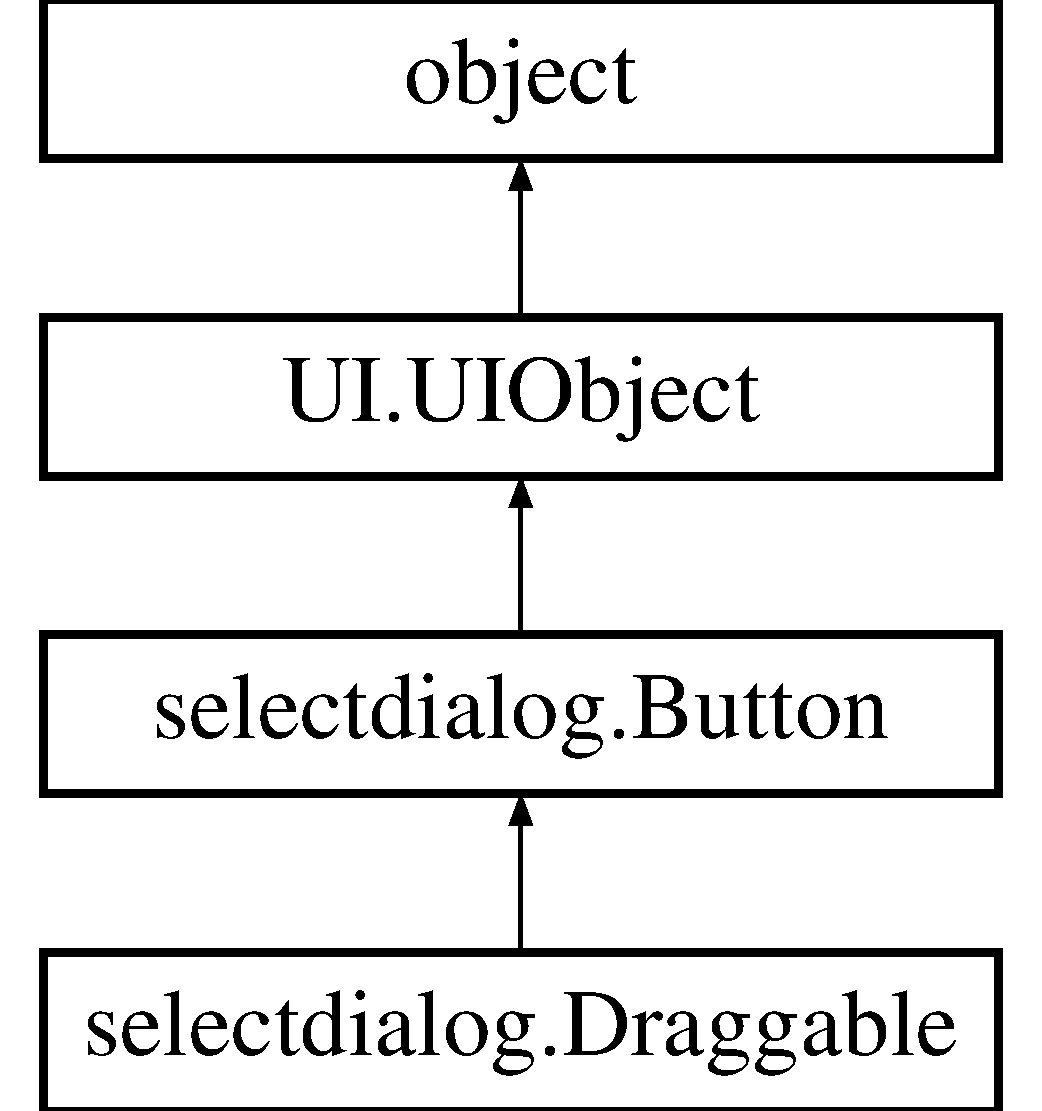
\includegraphics[height=4.000000cm]{classselectdialog_1_1Button}
\end{center}
\end{figure}
\subsection*{Public Member Functions}
\begin{DoxyCompactItemize}
\item 
\hypertarget{classselectdialog_1_1Button_a08071ed3d038becc84abdd009fdec51f}{def {\bfseries \-\_\-\-\_\-init\-\_\-\-\_\-}}\label{classselectdialog_1_1Button_a08071ed3d038becc84abdd009fdec51f}

\item 
\hypertarget{classselectdialog_1_1Button_a9c6db95e7982a93ba8f99826ebb0a8f0}{def {\bfseries event}}\label{classselectdialog_1_1Button_a9c6db95e7982a93ba8f99826ebb0a8f0}

\item 
\hypertarget{classselectdialog_1_1Button_a64806a7a8fe018d99f65008046e252fe}{def {\bfseries clicked}}\label{classselectdialog_1_1Button_a64806a7a8fe018d99f65008046e252fe}

\end{DoxyCompactItemize}
\subsection*{Data Fields}
\begin{DoxyCompactItemize}
\item 
\hypertarget{classselectdialog_1_1Button_a967a48ded59987a3bf29461b1e5259c1}{{\bfseries down}}\label{classselectdialog_1_1Button_a967a48ded59987a3bf29461b1e5259c1}

\end{DoxyCompactItemize}
\subsection*{Additional Inherited Members}


\subsection{Detailed Description}


Definition at line 75 of file selectdialog.\-py.



The documentation for this class was generated from the following file\-:\begin{DoxyCompactItemize}
\item 
/home/antipant/\-Protocol\-P\-\_\-\-Project/\-U\-I/selectdialog.\-py\end{DoxyCompactItemize}

\hypertarget{classUI_1_1Button}{\section{U\-I.\-Button Class Reference}
\label{classUI_1_1Button}\index{U\-I.\-Button@{U\-I.\-Button}}
}
Inheritance diagram for U\-I.\-Button\-:\begin{figure}[H]
\begin{center}
\leavevmode
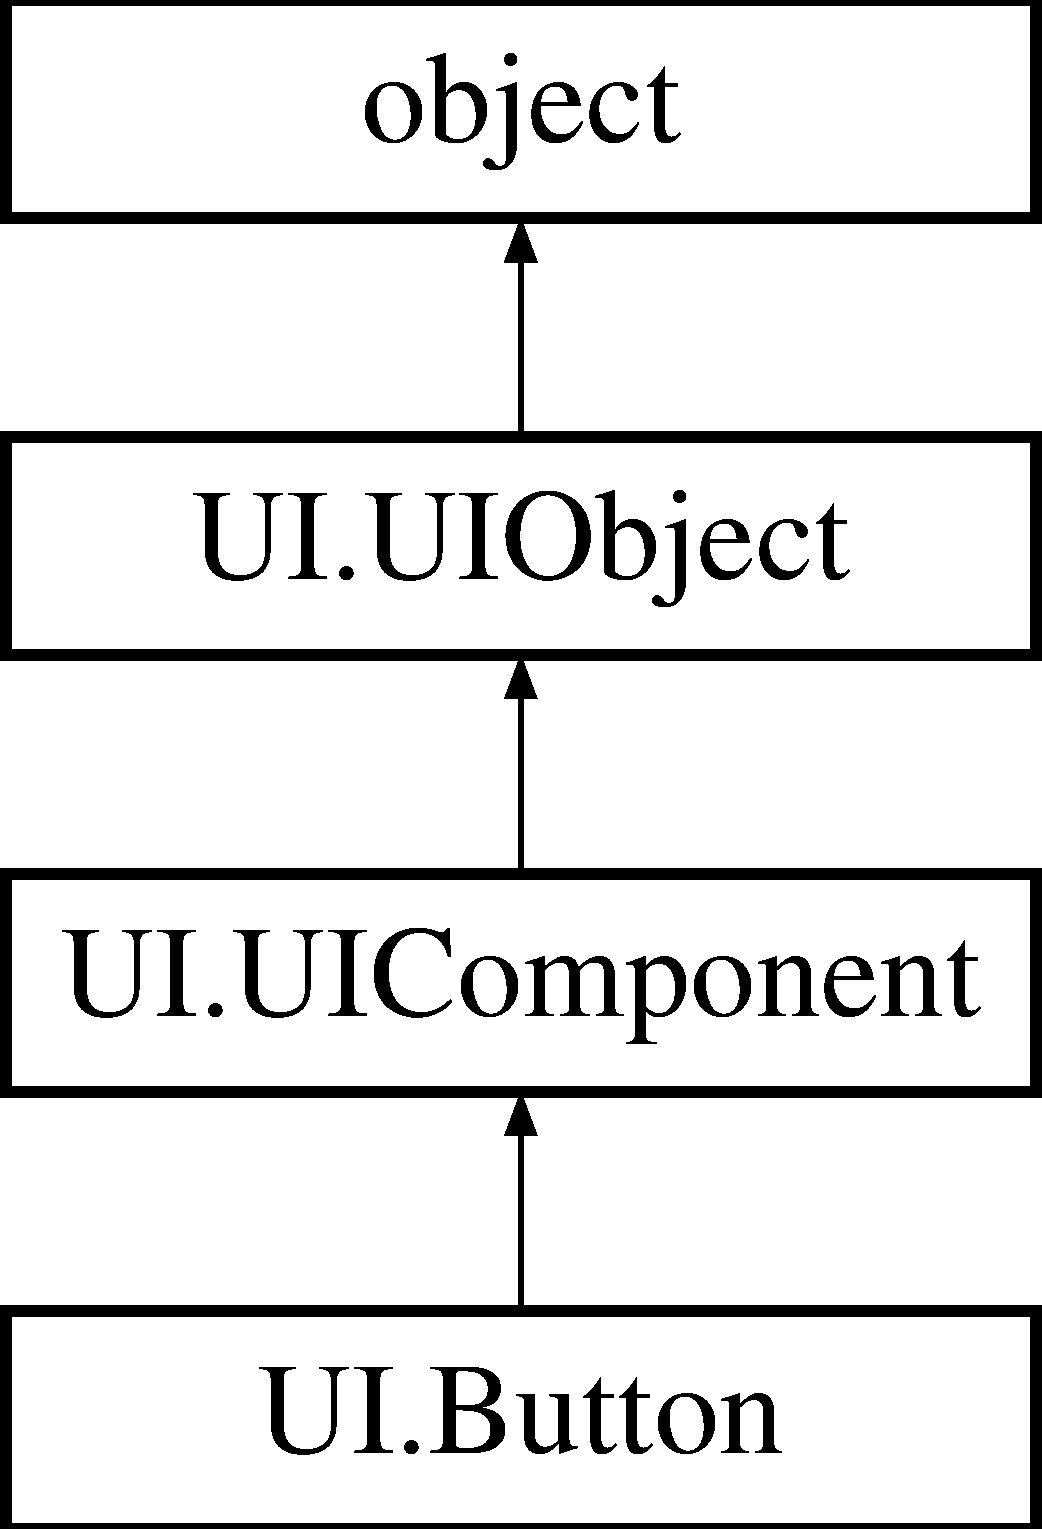
\includegraphics[height=4.000000cm]{classUI_1_1Button}
\end{center}
\end{figure}
\subsection*{Public Member Functions}
\begin{DoxyCompactItemize}
\item 
\hypertarget{classUI_1_1Button_aaffec11c22af344f6ff1dd12f64e1f76}{def {\bfseries \-\_\-\-\_\-init\-\_\-\-\_\-}}\label{classUI_1_1Button_aaffec11c22af344f6ff1dd12f64e1f76}

\item 
\hypertarget{classUI_1_1Button_a56560e47f3fe9a13deb863c8ae9f6370}{def {\bfseries button\-\_\-click}}\label{classUI_1_1Button_a56560e47f3fe9a13deb863c8ae9f6370}

\item 
\hypertarget{classUI_1_1Button_ae48553708f8cf5e878166f60d81a5999}{def {\bfseries enable\-\_\-buttons}}\label{classUI_1_1Button_ae48553708f8cf5e878166f60d81a5999}

\end{DoxyCompactItemize}
\subsection*{Data Fields}
\begin{DoxyCompactItemize}
\item 
\hypertarget{classUI_1_1Button_a959c354ded4f8a42b89d97e4abe7dc9b}{{\bfseries parent}}\label{classUI_1_1Button_a959c354ded4f8a42b89d97e4abe7dc9b}

\item 
\hypertarget{classUI_1_1Button_a2cd52c8b258fd7e839577692a85fc3ad}{{\bfseries surface}}\label{classUI_1_1Button_a2cd52c8b258fd7e839577692a85fc3ad}

\item 
\hypertarget{classUI_1_1Button_ac5647381d981b66e85f0d78fa6b5614f}{{\bfseries button}}\label{classUI_1_1Button_ac5647381d981b66e85f0d78fa6b5614f}

\end{DoxyCompactItemize}
\subsection*{Additional Inherited Members}


\subsection{Detailed Description}


Definition at line 377 of file U\-I.\-py.



The documentation for this class was generated from the following file\-:\begin{DoxyCompactItemize}
\item 
/home/antipant/\-Protocol\-P\-\_\-\-Project/\-U\-I/U\-I.\-py\end{DoxyCompactItemize}

\hypertarget{classUI_1_1CascadeButton}{\section{U\-I.\-Cascade\-Button Class Reference}
\label{classUI_1_1CascadeButton}\index{U\-I.\-Cascade\-Button@{U\-I.\-Cascade\-Button}}
}
Inheritance diagram for U\-I.\-Cascade\-Button\-:\begin{figure}[H]
\begin{center}
\leavevmode
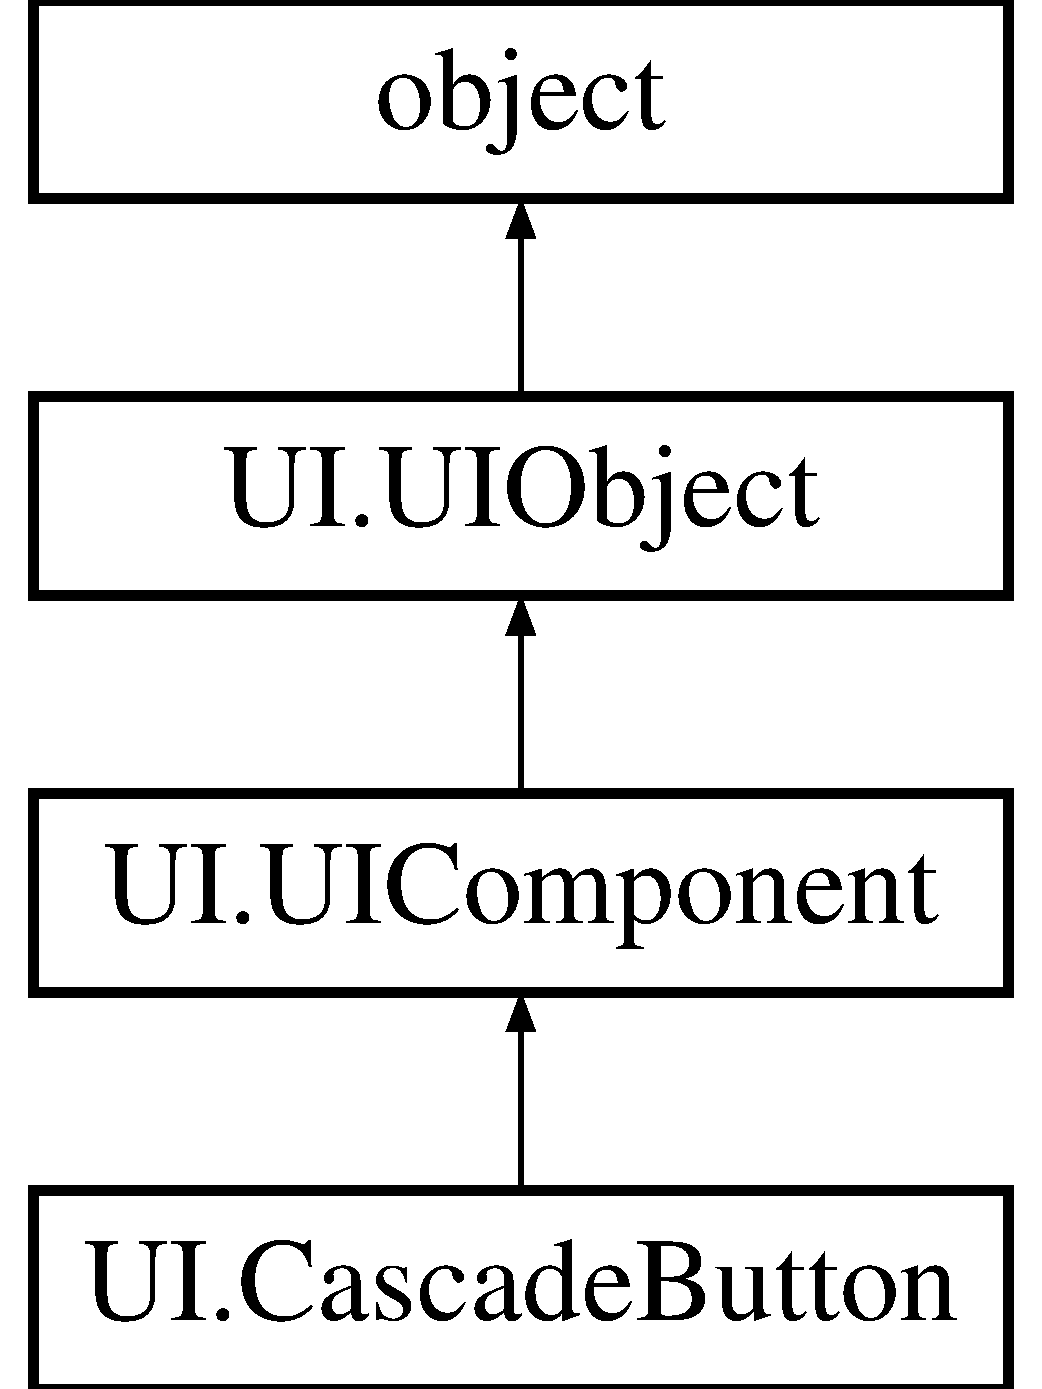
\includegraphics[height=4.000000cm]{classUI_1_1CascadeButton}
\end{center}
\end{figure}
\subsection*{Public Member Functions}
\begin{DoxyCompactItemize}
\item 
\hypertarget{classUI_1_1CascadeButton_a734e71bdf956a37ed998b16d470a9be4}{def {\bfseries \-\_\-\-\_\-init\-\_\-\-\_\-}}\label{classUI_1_1CascadeButton_a734e71bdf956a37ed998b16d470a9be4}

\item 
\hypertarget{classUI_1_1CascadeButton_a326430486252c04954c64fe4dae3ad23}{def {\bfseries add\-\_\-button}}\label{classUI_1_1CascadeButton_a326430486252c04954c64fe4dae3ad23}

\item 
\hypertarget{classUI_1_1CascadeButton_aad5dbe957f247572cd8d638f9f6898eb}{def {\bfseries button\-\_\-click}}\label{classUI_1_1CascadeButton_aad5dbe957f247572cd8d638f9f6898eb}

\item 
\hypertarget{classUI_1_1CascadeButton_a4a59c23b5d0ec44c62e9f4c22b665121}{def {\bfseries enable\-\_\-buttons}}\label{classUI_1_1CascadeButton_a4a59c23b5d0ec44c62e9f4c22b665121}

\item 
\hypertarget{classUI_1_1CascadeButton_aa438d1cd30daa5fd8ba545ccc2e8e077}{def {\bfseries hide\-\_\-buttons}}\label{classUI_1_1CascadeButton_aa438d1cd30daa5fd8ba545ccc2e8e077}

\end{DoxyCompactItemize}
\subsection*{Data Fields}
\begin{DoxyCompactItemize}
\item 
\hypertarget{classUI_1_1CascadeButton_ae06b29cead7a042f08a0262c7483680d}{{\bfseries parent}}\label{classUI_1_1CascadeButton_ae06b29cead7a042f08a0262c7483680d}

\item 
\hypertarget{classUI_1_1CascadeButton_a8906015ffd34eccc9a6c36badc491f13}{{\bfseries surface}}\label{classUI_1_1CascadeButton_a8906015ffd34eccc9a6c36badc491f13}

\item 
\hypertarget{classUI_1_1CascadeButton_aaf5d97877f96a4861f8cd22e655a93a1}{{\bfseries child\-\_\-buttons}}\label{classUI_1_1CascadeButton_aaf5d97877f96a4861f8cd22e655a93a1}

\item 
\hypertarget{classUI_1_1CascadeButton_a10390bcc6010c66da22e58b2ff5f6cae}{{\bfseries function}}\label{classUI_1_1CascadeButton_a10390bcc6010c66da22e58b2ff5f6cae}

\item 
\hypertarget{classUI_1_1CascadeButton_a7bb5bac8ce7670cf9e9d32f8a75c2fa1}{{\bfseries parent\-\_\-button}}\label{classUI_1_1CascadeButton_a7bb5bac8ce7670cf9e9d32f8a75c2fa1}

\item 
\hypertarget{classUI_1_1CascadeButton_a70230155e3d64cfda15110684e17308f}{{\bfseries name}}\label{classUI_1_1CascadeButton_a70230155e3d64cfda15110684e17308f}

\item 
\hypertarget{classUI_1_1CascadeButton_a3c834a67429959d420e20e32326b3287}{{\bfseries childs\-\_\-visible}}\label{classUI_1_1CascadeButton_a3c834a67429959d420e20e32326b3287}

\end{DoxyCompactItemize}
\subsection*{Additional Inherited Members}


\subsection{Detailed Description}


Definition at line 325 of file U\-I.\-py.



The documentation for this class was generated from the following file\-:\begin{DoxyCompactItemize}
\item 
/home/antipant/\-Protocol\-P\-\_\-\-Project/\-U\-I/U\-I.\-py\end{DoxyCompactItemize}

\hypertarget{classCommunication__If}{\section{Communication\-\_\-\-If Class Reference}
\label{classCommunication__If}\index{Communication\-\_\-\-If@{Communication\-\_\-\-If}}
}
Inheritance diagram for Communication\-\_\-\-If\-:\begin{figure}[H]
\begin{center}
\leavevmode
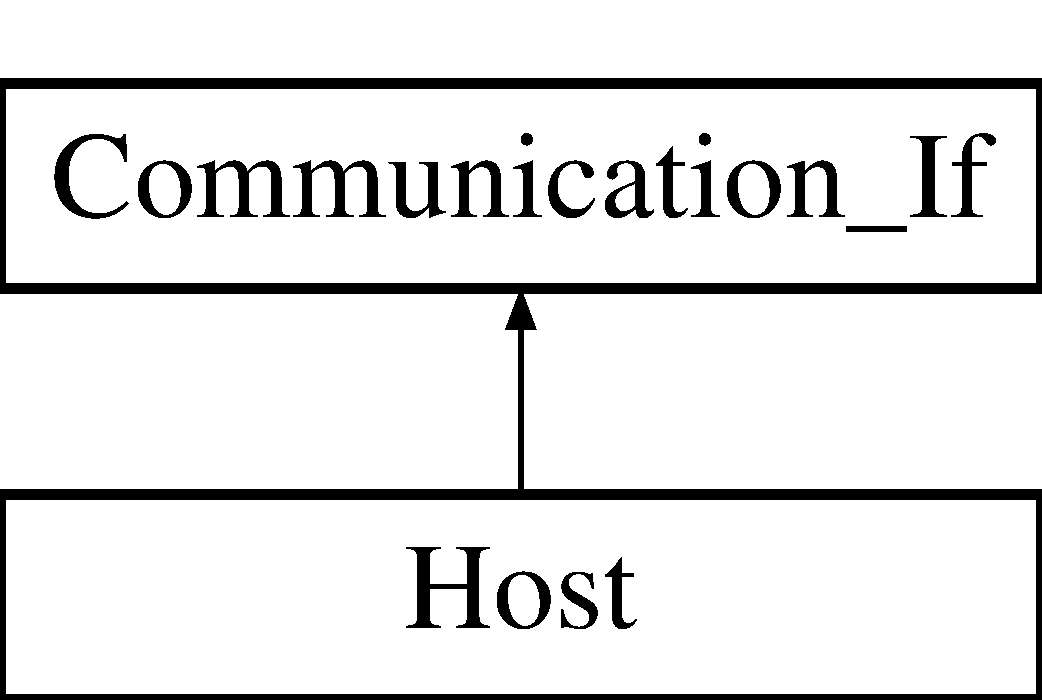
\includegraphics[height=2.000000cm]{classCommunication__If}
\end{center}
\end{figure}
\subsection*{Public Member Functions}
\begin{DoxyCompactItemize}
\item 
virtual bool \hyperlink{classCommunication__If_ab9c0279d64e4ce15b2f54c0df6d8ee3a}{send\-Message} (string p\-\_\-\-Destination\-I\-P, string p\-\_\-\-Source\-I\-P, string p\-\_\-\-Payload)=0
\begin{DoxyCompactList}\small\item\em Builds an I\-P packet using the passed fields as data. \end{DoxyCompactList}\item 
virtual string \hyperlink{classCommunication__If_a6a6083e9f88d3bd0897ccd1c6448f9c8}{rea\-Message\-Buffer} (void)=0
\begin{DoxyCompactList}\small\item\em Return the content of the message buffer string. \end{DoxyCompactList}\item 
\hypertarget{classCommunication__If_ad0a41ea2bebc146be6ee6db89d49486d}{virtual void \hyperlink{classCommunication__If_ad0a41ea2bebc146be6ee6db89d49486d}{clear\-Message\-Buffer} (void)=0}\label{classCommunication__If_ad0a41ea2bebc146be6ee6db89d49486d}

\begin{DoxyCompactList}\small\item\em Clears the message buffer string. \end{DoxyCompactList}\end{DoxyCompactItemize}


\subsection{Detailed Description}


Definition at line 30 of file Communication\-\_\-\-If.\-hpp.



\subsection{Member Function Documentation}
\hypertarget{classCommunication__If_a6a6083e9f88d3bd0897ccd1c6448f9c8}{\index{Communication\-\_\-\-If@{Communication\-\_\-\-If}!rea\-Message\-Buffer@{rea\-Message\-Buffer}}
\index{rea\-Message\-Buffer@{rea\-Message\-Buffer}!Communication_If@{Communication\-\_\-\-If}}
\subsubsection[{rea\-Message\-Buffer}]{\setlength{\rightskip}{0pt plus 5cm}string Communication\-\_\-\-If\-::rea\-Message\-Buffer (
\begin{DoxyParamCaption}
\item[{void}]{}
\end{DoxyParamCaption}
)\hspace{0.3cm}{\ttfamily [pure virtual]}}}\label{classCommunication__If_a6a6083e9f88d3bd0897ccd1c6448f9c8}


Return the content of the message buffer string. 

\begin{DoxyReturn}{Returns}
Message buffer string 
\end{DoxyReturn}


Implemented in \hyperlink{classHost_a4393bc6a6521e084d9f2663f8d0564bb}{Host}.

\hypertarget{classCommunication__If_ab9c0279d64e4ce15b2f54c0df6d8ee3a}{\index{Communication\-\_\-\-If@{Communication\-\_\-\-If}!send\-Message@{send\-Message}}
\index{send\-Message@{send\-Message}!Communication_If@{Communication\-\_\-\-If}}
\subsubsection[{send\-Message}]{\setlength{\rightskip}{0pt plus 5cm}bool Communication\-\_\-\-If\-::send\-Message (
\begin{DoxyParamCaption}
\item[{string}]{p\-\_\-\-Destination\-I\-P, }
\item[{string}]{p\-\_\-\-Source\-I\-P, }
\item[{string}]{p\-\_\-\-Payload}
\end{DoxyParamCaption}
)\hspace{0.3cm}{\ttfamily [pure virtual]}}}\label{classCommunication__If_ab9c0279d64e4ce15b2f54c0df6d8ee3a}


Builds an I\-P packet using the passed fields as data. 


\begin{DoxyParams}[1]{Parameters}
\mbox{\tt in}  & {\em string} & p\-\_\-\-Destination\-I\-P \\
\hline
\mbox{\tt in}  & {\em string} & p\-\_\-\-Source\-I\-P \\
\hline
\mbox{\tt in}  & {\em string} & p\-\_\-\-Payload \\
\hline
\end{DoxyParams}
\begin{DoxyReturn}{Returns}
bool true\-: message send succeeded -\/ false\-: error 
\end{DoxyReturn}


Implemented in \hyperlink{classHost_a56eb630fcf00ef1184d5df27f66a9b9e}{Host}.



The documentation for this class was generated from the following file\-:\begin{DoxyCompactItemize}
\item 
/home/antipant/\-Protocol\-P\-\_\-\-Project/\hyperlink{Communication__If_8hpp}{Communication\-\_\-\-If.\-hpp}\end{DoxyCompactItemize}

\hypertarget{classConnection}{\section{Connection Class Reference}
\label{classConnection}\index{Connection@{Connection}}
}


Holds the connection parameters for local interface.  




{\ttfamily \#include $<$Configuration.\-hpp$>$}

\subsection*{Public Member Functions}
\begin{DoxyCompactItemize}
\item 
\hypertarget{classConnection_a9686aa58b79ed0eed5ae0d4d2e67f063}{{\bfseries Connection} (int p\-\_\-\-Neighbor\-Interface\-Id, int p\-\_\-\-Neighbor\-Router\-Id)}\label{classConnection_a9686aa58b79ed0eed5ae0d4d2e67f063}

\item 
\hypertarget{classConnection_ac29c2a46399ef547746c308a74cda281}{void {\bfseries set\-Neighbor\-Router\-Id} (int p\-\_\-\-Neighbor\-Router\-Id)}\label{classConnection_ac29c2a46399ef547746c308a74cda281}

\item 
\hypertarget{classConnection_ab782704880dbb2a09dcdaf32ffc933fa}{void {\bfseries set\-Neighbor\-Interface\-Id} (int p\-\_\-\-Neighbor\-Interface\-Id)}\label{classConnection_ab782704880dbb2a09dcdaf32ffc933fa}

\item 
\hypertarget{classConnection_ac8c1278f4bef13f4ff468b14bef20c87}{int {\bfseries get\-Neighbor\-Router\-Id} (void)}\label{classConnection_ac8c1278f4bef13f4ff468b14bef20c87}

\item 
\hypertarget{classConnection_a67d5ae99b81ceb7544d20a440564041d}{int {\bfseries get\-Neighbor\-Interface\-Id} (void)}\label{classConnection_a67d5ae99b81ceb7544d20a440564041d}

\item 
\hypertarget{classConnection_ac70c6b1d8968a356e3da41f0b5db130d}{bool {\bfseries has\-Connection} (void)}\label{classConnection_ac70c6b1d8968a356e3da41f0b5db130d}

\item 
\hypertarget{classConnection_adfe081e8f1870d3fed68fe9a87fb5775}{string {\bfseries to\-String} (void)}\label{classConnection_adfe081e8f1870d3fed68fe9a87fb5775}

\end{DoxyCompactItemize}
\subsection*{Data Fields}
\begin{DoxyCompactItemize}
\item 
\hypertarget{classConnection_aa025764cb3ec8317eebf40b4c92f0551}{int \hyperlink{classConnection_aa025764cb3ec8317eebf40b4c92f0551}{m\-\_\-\-Neighbor\-Interface\-Id}}\label{classConnection_aa025764cb3ec8317eebf40b4c92f0551}

\begin{DoxyCompactList}\small\item\em The id of the neighbor interface to where this router connects. \end{DoxyCompactList}\item 
\hypertarget{classConnection_a0c3cc5f16fa26d798d63472a309185cb}{int \hyperlink{classConnection_a0c3cc5f16fa26d798d63472a309185cb}{m\-\_\-\-Neighbor\-Router\-Id}}\label{classConnection_a0c3cc5f16fa26d798d63472a309185cb}

\begin{DoxyCompactList}\small\item\em The id of the neighbor router on which the neighbor interface is located. \end{DoxyCompactList}\end{DoxyCompactItemize}


\subsection{Detailed Description}
Holds the connection parameters for local interface. 

Definition at line 378 of file Configuration.\-hpp.



The documentation for this class was generated from the following files\-:\begin{DoxyCompactItemize}
\item 
/home/antipant/\-Protocol\-P\-\_\-\-Project/\hyperlink{Configuration_8hpp}{Configuration.\-hpp}\item 
/home/antipant/\-Protocol\-P\-\_\-\-Project/\hyperlink{Configuration_8cpp}{Configuration.\-cpp}\end{DoxyCompactItemize}

\hypertarget{classSimulationUI_1_1Console}{\section{Simulation\-U\-I.\-Console Class Reference}
\label{classSimulationUI_1_1Console}\index{Simulation\-U\-I.\-Console@{Simulation\-U\-I.\-Console}}
}
\subsection*{Public Member Functions}
\begin{DoxyCompactItemize}
\item 
\hypertarget{classSimulationUI_1_1Console_a5de1c29e64e0559fc6f5b69ff22cb892}{def {\bfseries \-\_\-\-\_\-init\-\_\-\-\_\-}}\label{classSimulationUI_1_1Console_a5de1c29e64e0559fc6f5b69ff22cb892}

\item 
\hypertarget{classSimulationUI_1_1Console_a09250d473ecb6e32cf34c980f0c3de03}{def {\bfseries send}}\label{classSimulationUI_1_1Console_a09250d473ecb6e32cf34c980f0c3de03}

\item 
\hypertarget{classSimulationUI_1_1Console_a6f9d846cbd66a681b3f18294bee80c01}{def {\bfseries add\-\_\-log}}\label{classSimulationUI_1_1Console_a6f9d846cbd66a681b3f18294bee80c01}

\end{DoxyCompactItemize}
\subsection*{Data Fields}
\begin{DoxyCompactItemize}
\item 
\hypertarget{classSimulationUI_1_1Console_a9f59684b680f0d9877deaa446603b317}{{\bfseries log}}\label{classSimulationUI_1_1Console_a9f59684b680f0d9877deaa446603b317}

\item 
\hypertarget{classSimulationUI_1_1Console_a0b802bbad21c9f03c1dba08f4dc0e7ce}{{\bfseries prompt}}\label{classSimulationUI_1_1Console_a0b802bbad21c9f03c1dba08f4dc0e7ce}

\end{DoxyCompactItemize}


\subsection{Detailed Description}


Definition at line 204 of file Simulation\-U\-I.\-py.



The documentation for this class was generated from the following file\-:\begin{DoxyCompactItemize}
\item 
/home/antipant/\-Protocol\-P\-\_\-\-Project/\-U\-I/Simulation\-U\-I.\-py\end{DoxyCompactItemize}

\hypertarget{classControlPlane}{\section{Control\-Plane Class Reference}
\label{classControlPlane}\index{Control\-Plane@{Control\-Plane}}
}


\hyperlink{classControlPlane}{Control\-Plane} module runs the B\-G\-P process.  




{\ttfamily \#include $<$Control\-Plane.\-hpp$>$}

Inheritance diagram for Control\-Plane\-:\begin{figure}[H]
\begin{center}
\leavevmode
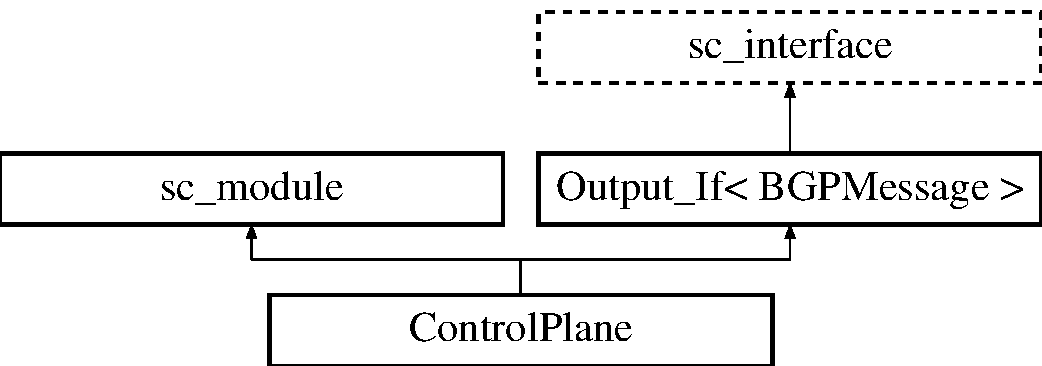
\includegraphics[height=3.000000cm]{classControlPlane}
\end{center}
\end{figure}
\subsection*{Public Member Functions}
\begin{DoxyCompactItemize}
\item 
\hypertarget{classControlPlane_a5f1b4e4cd901efc31af6d97b325b2a50}{void {\bfseries before\-\_\-end\-\_\-of\-\_\-elaboration} ()}\label{classControlPlane_a5f1b4e4cd901efc31af6d97b325b2a50}

\item 
\hypertarget{classControlPlane_a03b8627e5a45efd3c5b1cdcdfc36257d}{\hyperlink{classControlPlane_a03b8627e5a45efd3c5b1cdcdfc36257d}{Control\-Plane} (sc\-\_\-module\-\_\-name p\-\_\-\-Mod\-Name, \hyperlink{classControlPlaneConfig}{Control\-Plane\-Config} $\ast$const p\-\_\-\-B\-G\-P\-Config)}\label{classControlPlane_a03b8627e5a45efd3c5b1cdcdfc36257d}

\begin{DoxyCompactList}\small\item\em Elaborates the \hyperlink{classControlPlane}{Control\-Plane} module. \end{DoxyCompactList}\item 
\hyperlink{classControlPlane_a89e252e0ec65d15f1b9cc3a1248c6875}{$\sim$\-Control\-Plane} ()
\begin{DoxyCompactList}\small\item\em Destructor of the \hyperlink{classControlPlane}{Control\-Plane} module. \end{DoxyCompactList}\item 
void \hyperlink{classControlPlane_af1439606467be6968d9b8bc74e797c9b}{control\-Plane\-Main} (void)
\begin{DoxyCompactList}\small\item\em The main process of Control Plane module. \end{DoxyCompactList}\item 
virtual bool \hyperlink{classControlPlane_a602bc55e4d99aab6e0b38468afecdc1f}{write} (\hyperlink{classBGPMessage}{B\-G\-P\-Message} \&p\-\_\-\-B\-G\-P\-Msg)
\item 
\hypertarget{classControlPlane_a75d7a33d6f0ce90d016fc5834e946d89}{void {\bfseries kill\-Control\-Plane} (void)}\label{classControlPlane_a75d7a33d6f0ce90d016fc5834e946d89}

\item 
\hypertarget{classControlPlane_ab1d2f0ce243546442eedf76053811154}{void {\bfseries set\-Up} (bool p\-\_\-\-Value)}\label{classControlPlane_ab1d2f0ce243546442eedf76053811154}

\item 
\hypertarget{classControlPlane_a0b791170af33147760ae97cec79dfe68}{void {\bfseries revive\-Control\-Plane} (void)}\label{classControlPlane_a0b791170af33147760ae97cec79dfe68}

\item 
\hypertarget{classControlPlane_aad1a701de61f52e2827a37250ec35048}{bool {\bfseries is\-Running} (void)}\label{classControlPlane_aad1a701de61f52e2827a37250ec35048}

\item 
\hyperlink{classControlPlane_a1ea8212be6d995f37ea9bc42c0f0adc2}{S\-C\-\_\-\-H\-A\-S\-\_\-\-P\-R\-O\-C\-E\-S\-S} (\hyperlink{classControlPlane}{Control\-Plane})
\begin{DoxyCompactList}\small\item\em Indicate the system\-C producer that this module has a process. \end{DoxyCompactList}\end{DoxyCompactItemize}
\subsection*{Data Fields}
\begin{DoxyCompactItemize}
\item 
sc\-\_\-in\-\_\-clk \hyperlink{classControlPlane_ab0c4f01f5a65a86750cc4011bc531b70}{port\-\_\-\-Clk}
\begin{DoxyCompactList}\small\item\em System clock signal. \end{DoxyCompactList}\item 
sc\-\_\-port$<$ \hyperlink{classOutput__If}{Output\-\_\-\-If}$<$ \hyperlink{classBGPMessage}{B\-G\-P\-Message} $>$\\*
,0, S\-C\-\_\-\-Z\-E\-R\-O\-\_\-\-O\-R\-\_\-\-M\-O\-R\-E\-\_\-\-B\-O\-U\-N\-D $>$ \hyperlink{classControlPlane_adff1abdc123100e569d92ce1485a378e}{port\-\_\-\-To\-Data\-Plane}
\begin{DoxyCompactList}\small\item\em Forwarding port. \end{DoxyCompactList}\item 
\hypertarget{classControlPlane_a76e565e9e2be198c1d67944db521f466}{sc\-\_\-export$<$ \hyperlink{classInterface__If}{Interface\-\_\-\-If} $>$ $\ast$$\ast$ \hyperlink{classControlPlane_a76e565e9e2be198c1d67944db521f466}{export\-\_\-\-Interface\-Control}}\label{classControlPlane_a76e565e9e2be198c1d67944db521f466}

\begin{DoxyCompactList}\small\item\em N\-I\-C control port. \end{DoxyCompactList}\item 
sc\-\_\-export$<$ \hyperlink{classOutput__If}{Output\-\_\-\-If}\\*
$<$ \hyperlink{classBGPMessage}{B\-G\-P\-Message} $>$ $>$ $\ast$$\ast$ \hyperlink{classControlPlane_a7045b3cc322a96eed95d40df9e388964}{export\-\_\-\-Routing\-Table}
\begin{DoxyCompactList}\small\item\em Routing table If. \end{DoxyCompactList}\item 
sc\-\_\-export$<$ sc\-\_\-fifo\-\_\-out\-\_\-if\\*
$<$ \hyperlink{classBGPMessage}{B\-G\-P\-Message} $>$ $>$ \hyperlink{classControlPlane_a8eeed022eec78d21f65728c01490684e}{export\-\_\-\-To\-Control\-Plane}
\begin{DoxyCompactList}\small\item\em Input interface. \end{DoxyCompactList}\item 
\hypertarget{classControlPlane_a69d5761d8047ee6e73f7b539cf8676a0}{sc\-\_\-export$<$ \hyperlink{classBGPSession__If}{B\-G\-P\-Session\-\_\-\-If} $>$ $\ast$$\ast$ {\bfseries export\-\_\-\-Session}}\label{classControlPlane_a69d5761d8047ee6e73f7b539cf8676a0}

\item 
\hypertarget{classControlPlane_a2ea2be172ff69fd4e7260a0c853edfb6}{sc\-\_\-export$<$ \hyperlink{classOutput__If}{Output\-\_\-\-If}\\*
$<$ \hyperlink{classBGPMessage}{B\-G\-P\-Message} $>$ $>$ \hyperlink{classControlPlane_a2ea2be172ff69fd4e7260a0c853edfb6}{export\-\_\-\-To\-Data\-Plane}}\label{classControlPlane_a2ea2be172ff69fd4e7260a0c853edfb6}

\begin{DoxyCompactList}\small\item\em This provides the Data\-Plane\-\_\-\-In\-\_\-\-If for B\-G\-P sessions. \end{DoxyCompactList}\end{DoxyCompactItemize}


\subsection{Detailed Description}
\hyperlink{classControlPlane}{Control\-Plane} module runs the B\-G\-P process. 

Definition at line 38 of file Control\-Plane.\-hpp.



\subsection{Constructor \& Destructor Documentation}
\hypertarget{classControlPlane_a89e252e0ec65d15f1b9cc3a1248c6875}{\index{Control\-Plane@{Control\-Plane}!$\sim$\-Control\-Plane@{$\sim$\-Control\-Plane}}
\index{$\sim$\-Control\-Plane@{$\sim$\-Control\-Plane}!ControlPlane@{Control\-Plane}}
\subsubsection[{$\sim$\-Control\-Plane}]{\setlength{\rightskip}{0pt plus 5cm}Control\-Plane\-::$\sim$\-Control\-Plane (
\begin{DoxyParamCaption}
{}
\end{DoxyParamCaption}
)}}\label{classControlPlane_a89e252e0ec65d15f1b9cc3a1248c6875}


Destructor of the \hyperlink{classControlPlane}{Control\-Plane} module. 

Free's all the dynamically allocated memory 

Definition at line 50 of file Control\-Plane.\-cpp.



\subsection{Member Function Documentation}
\hypertarget{classControlPlane_af1439606467be6968d9b8bc74e797c9b}{\index{Control\-Plane@{Control\-Plane}!control\-Plane\-Main@{control\-Plane\-Main}}
\index{control\-Plane\-Main@{control\-Plane\-Main}!ControlPlane@{Control\-Plane}}
\subsubsection[{control\-Plane\-Main}]{\setlength{\rightskip}{0pt plus 5cm}void Control\-Plane\-::control\-Plane\-Main (
\begin{DoxyParamCaption}
\item[{void}]{}
\end{DoxyParamCaption}
)}}\label{classControlPlane_af1439606467be6968d9b8bc74e797c9b}


The main process of Control Plane module. 

\begin{DoxyItemize}
\item Reads B\-G\-P messages from the m\-\_\-\-Receiving\-Buffer.\item performs the route resolution process accoriding to B\-G\-P protocol. \item Generates the required update messages.\item Keeps track on different B\-G\-P sessions. \end{DoxyItemize}


Definition at line 60 of file Control\-Plane.\-cpp.

\hypertarget{classControlPlane_a1ea8212be6d995f37ea9bc42c0f0adc2}{\index{Control\-Plane@{Control\-Plane}!S\-C\-\_\-\-H\-A\-S\-\_\-\-P\-R\-O\-C\-E\-S\-S@{S\-C\-\_\-\-H\-A\-S\-\_\-\-P\-R\-O\-C\-E\-S\-S}}
\index{S\-C\-\_\-\-H\-A\-S\-\_\-\-P\-R\-O\-C\-E\-S\-S@{S\-C\-\_\-\-H\-A\-S\-\_\-\-P\-R\-O\-C\-E\-S\-S}!ControlPlane@{Control\-Plane}}
\subsubsection[{S\-C\-\_\-\-H\-A\-S\-\_\-\-P\-R\-O\-C\-E\-S\-S}]{\setlength{\rightskip}{0pt plus 5cm}Control\-Plane\-::\-S\-C\-\_\-\-H\-A\-S\-\_\-\-P\-R\-O\-C\-E\-S\-S (
\begin{DoxyParamCaption}
\item[{{\bf Control\-Plane}}]{}
\end{DoxyParamCaption}
)}}\label{classControlPlane_a1ea8212be6d995f37ea9bc42c0f0adc2}


Indicate the system\-C producer that this module has a process. 

\begin{DoxySeeAlso}{See Also}
\href{http://www.iro.umontreal.ca/~lablasso/docs/SystemC2.0.1/html/classproducer.html}{\tt http\-://www.\-iro.\-umontreal.\-ca/$\sim$lablasso/docs/\-System\-C2.\-0.\-1/html/classproducer.\-html} 
\end{DoxySeeAlso}
\hypertarget{classControlPlane_a602bc55e4d99aab6e0b38468afecdc1f}{\index{Control\-Plane@{Control\-Plane}!write@{write}}
\index{write@{write}!ControlPlane@{Control\-Plane}}
\subsubsection[{write}]{\setlength{\rightskip}{0pt plus 5cm}bool Control\-Plane\-::write (
\begin{DoxyParamCaption}
\item[{{\bf B\-G\-P\-Message} \&}]{p\-\_\-\-B\-G\-P\-Msg}
\end{DoxyParamCaption}
)\hspace{0.3cm}{\ttfamily [virtual]}}}\label{classControlPlane_a602bc55e4d99aab6e0b38468afecdc1f}
\begin{DoxySeeAlso}{See Also}
\hyperlink{classOutput__If}{Output\-\_\-\-If} 
\end{DoxySeeAlso}


Implements \hyperlink{classOutput__If_aeef0f3dff2d02e85375e914e83140602}{Output\-\_\-\-If$<$ B\-G\-P\-Message $>$}.



Definition at line 121 of file Control\-Plane.\-cpp.



\subsection{Field Documentation}
\hypertarget{classControlPlane_a7045b3cc322a96eed95d40df9e388964}{\index{Control\-Plane@{Control\-Plane}!export\-\_\-\-Routing\-Table@{export\-\_\-\-Routing\-Table}}
\index{export\-\_\-\-Routing\-Table@{export\-\_\-\-Routing\-Table}!ControlPlane@{Control\-Plane}}
\subsubsection[{export\-\_\-\-Routing\-Table}]{\setlength{\rightskip}{0pt plus 5cm}sc\-\_\-export$<${\bf Output\-\_\-\-If}$<${\bf B\-G\-P\-Message}$>$ $>$$\ast$$\ast$ Control\-Plane\-::export\-\_\-\-Routing\-Table}}\label{classControlPlane_a7045b3cc322a96eed95d40df9e388964}


Routing table If. 

exports the output\-\_\-if of routing table for \hyperlink{classBGPSession}{B\-G\-P\-Session} 

Definition at line 66 of file Control\-Plane.\-hpp.

\hypertarget{classControlPlane_a8eeed022eec78d21f65728c01490684e}{\index{Control\-Plane@{Control\-Plane}!export\-\_\-\-To\-Control\-Plane@{export\-\_\-\-To\-Control\-Plane}}
\index{export\-\_\-\-To\-Control\-Plane@{export\-\_\-\-To\-Control\-Plane}!ControlPlane@{Control\-Plane}}
\subsubsection[{export\-\_\-\-To\-Control\-Plane}]{\setlength{\rightskip}{0pt plus 5cm}sc\-\_\-export$<$sc\-\_\-fifo\-\_\-out\-\_\-if$<${\bf B\-G\-P\-Message}$>$ $>$ Control\-Plane\-::export\-\_\-\-To\-Control\-Plane}}\label{classControlPlane_a8eeed022eec78d21f65728c01490684e}


Input interface. 

Allows data plane to write received B\-G\-P messages into m\-\_\-\-Receiving\-Buffer-\/fifo 

Definition at line 75 of file Control\-Plane.\-hpp.

\hypertarget{classControlPlane_ab0c4f01f5a65a86750cc4011bc531b70}{\index{Control\-Plane@{Control\-Plane}!port\-\_\-\-Clk@{port\-\_\-\-Clk}}
\index{port\-\_\-\-Clk@{port\-\_\-\-Clk}!ControlPlane@{Control\-Plane}}
\subsubsection[{port\-\_\-\-Clk}]{\setlength{\rightskip}{0pt plus 5cm}sc\-\_\-in\-\_\-clk Control\-Plane\-::port\-\_\-\-Clk}}\label{classControlPlane_ab0c4f01f5a65a86750cc4011bc531b70}


System clock signal. 

The router's internal clock 

Definition at line 48 of file Control\-Plane.\-hpp.

\hypertarget{classControlPlane_adff1abdc123100e569d92ce1485a378e}{\index{Control\-Plane@{Control\-Plane}!port\-\_\-\-To\-Data\-Plane@{port\-\_\-\-To\-Data\-Plane}}
\index{port\-\_\-\-To\-Data\-Plane@{port\-\_\-\-To\-Data\-Plane}!ControlPlane@{Control\-Plane}}
\subsubsection[{port\-\_\-\-To\-Data\-Plane}]{\setlength{\rightskip}{0pt plus 5cm}sc\-\_\-port$<${\bf Output\-\_\-\-If}$<${\bf B\-G\-P\-Message}$>$ ,0, S\-C\-\_\-\-Z\-E\-R\-O\-\_\-\-O\-R\-\_\-\-M\-O\-R\-E\-\_\-\-B\-O\-U\-N\-D$>$ Control\-Plane\-::port\-\_\-\-To\-Data\-Plane}}\label{classControlPlane_adff1abdc123100e569d92ce1485a378e}


Forwarding port. 

Used to write B\-G\-P messages to the data plane 

Definition at line 54 of file Control\-Plane.\-hpp.



The documentation for this class was generated from the following files\-:\begin{DoxyCompactItemize}
\item 
/home/antipant/\-Protocol\-P\-\_\-\-Project/\hyperlink{ControlPlane_8hpp}{Control\-Plane.\-hpp}\item 
/home/antipant/\-Protocol\-P\-\_\-\-Project/\hyperlink{ControlPlane_8cpp}{Control\-Plane.\-cpp}\end{DoxyCompactItemize}

\hypertarget{classControlPlaneConfig}{\section{Control\-Plane\-Config Class Reference}
\label{classControlPlaneConfig}\index{Control\-Plane\-Config@{Control\-Plane\-Config}}
}


Holds the B\-G\-P parameters.  




{\ttfamily \#include $<$Configuration.\-hpp$>$}

Inheritance diagram for Control\-Plane\-Config\-:\begin{figure}[H]
\begin{center}
\leavevmode
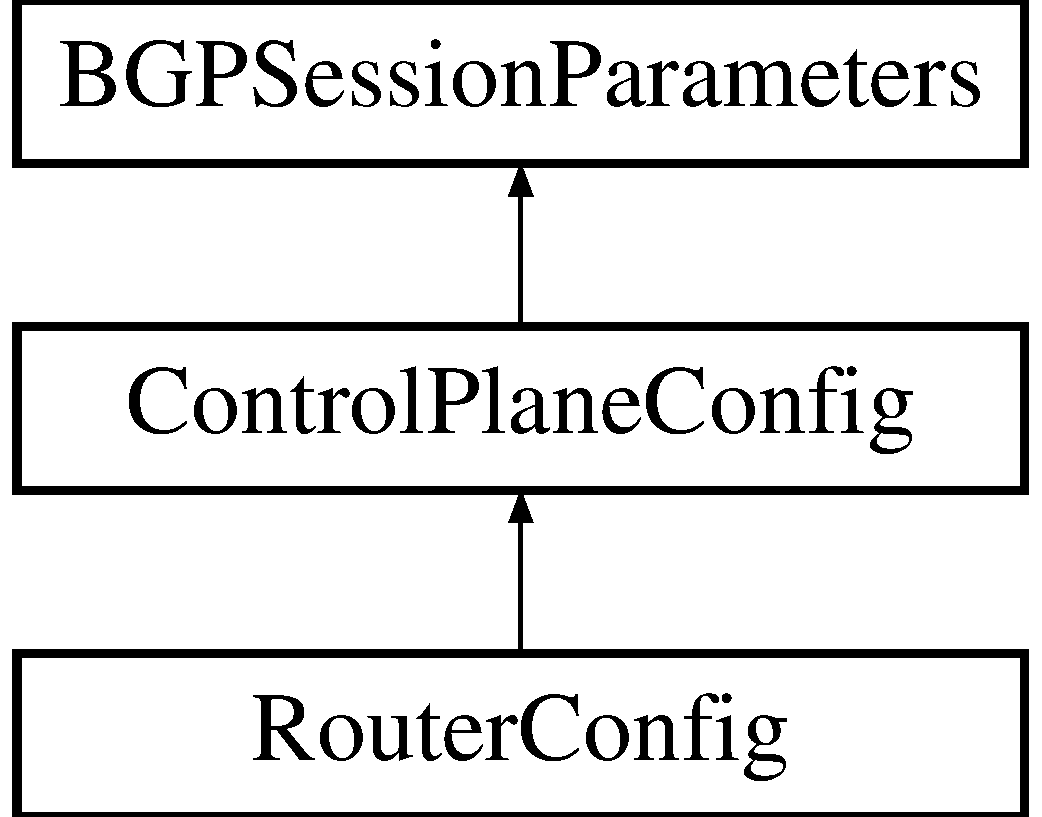
\includegraphics[height=3.000000cm]{classControlPlaneConfig}
\end{center}
\end{figure}
\subsection*{Public Member Functions}
\begin{DoxyCompactItemize}
\item 
void \hyperlink{classControlPlaneConfig_a75ca255e856818f3593111c6bc06b6c9}{set\-Number\-Of\-Interfaces} (int p\-\_\-\-Number\-Of\-Interfaces)
\begin{DoxyCompactList}\small\item\em Setters. \end{DoxyCompactList}\item 
int \hyperlink{classControlPlaneConfig_aa740ccf69f47b148711f8091aa672f31}{get\-Number\-Of\-Interfaces} (void)
\begin{DoxyCompactList}\small\item\em Getters. \end{DoxyCompactList}\item 
\hyperlink{classControlPlaneConfig}{Control\-Plane\-Config} \& \hyperlink{classControlPlaneConfig_aee06e39d17e552e41d8fc0a88580a022}{operator=} (const \hyperlink{classControlPlaneConfig}{Control\-Plane\-Config} \&p\-\_\-\-Original)
\begin{DoxyCompactList}\small\item\em clones the passed Controlplane\-Config object to this object \end{DoxyCompactList}\end{DoxyCompactItemize}
\subsection*{Protected Attributes}
\begin{DoxyCompactItemize}
\item 
\hypertarget{classControlPlaneConfig_a2a1c880c1616fe557e4f01a49decc1f2}{int \hyperlink{classControlPlaneConfig_a2a1c880c1616fe557e4f01a49decc1f2}{m\-\_\-\-Number\-Of\-Interfaces}}\label{classControlPlaneConfig_a2a1c880c1616fe557e4f01a49decc1f2}

\begin{DoxyCompactList}\small\item\em Number of network interfaces that this router should allocate. \end{DoxyCompactList}\end{DoxyCompactItemize}
\subsection*{Additional Inherited Members}


\subsection{Detailed Description}
Holds the B\-G\-P parameters. 

Definition at line 331 of file Configuration.\-hpp.



\subsection{Member Function Documentation}
\hypertarget{classControlPlaneConfig_aa740ccf69f47b148711f8091aa672f31}{\index{Control\-Plane\-Config@{Control\-Plane\-Config}!get\-Number\-Of\-Interfaces@{get\-Number\-Of\-Interfaces}}
\index{get\-Number\-Of\-Interfaces@{get\-Number\-Of\-Interfaces}!ControlPlaneConfig@{Control\-Plane\-Config}}
\subsubsection[{get\-Number\-Of\-Interfaces}]{\setlength{\rightskip}{0pt plus 5cm}int Control\-Plane\-Config\-::get\-Number\-Of\-Interfaces (
\begin{DoxyParamCaption}
\item[{void}]{}
\end{DoxyParamCaption}
)}}\label{classControlPlaneConfig_aa740ccf69f47b148711f8091aa672f31}


Getters. 

Returns the number of interface.

\begin{DoxyReturn}{Returns}
integer value 
\end{DoxyReturn}


Definition at line 161 of file Configuration.\-cpp.

\hypertarget{classControlPlaneConfig_aee06e39d17e552e41d8fc0a88580a022}{\index{Control\-Plane\-Config@{Control\-Plane\-Config}!operator=@{operator=}}
\index{operator=@{operator=}!ControlPlaneConfig@{Control\-Plane\-Config}}
\subsubsection[{operator=}]{\setlength{\rightskip}{0pt plus 5cm}{\bf Control\-Plane\-Config} \& Control\-Plane\-Config\-::operator= (
\begin{DoxyParamCaption}
\item[{const {\bf Control\-Plane\-Config} \&}]{p\-\_\-\-Original}
\end{DoxyParamCaption}
)}}\label{classControlPlaneConfig_aee06e39d17e552e41d8fc0a88580a022}


clones the passed Controlplane\-Config object to this object 

\begin{DoxyReturn}{Returns}
reference \hyperlink{classControlPlaneConfig}{Control\-Plane\-Config}\& 
\end{DoxyReturn}


Definition at line 164 of file Configuration.\-cpp.

\hypertarget{classControlPlaneConfig_a75ca255e856818f3593111c6bc06b6c9}{\index{Control\-Plane\-Config@{Control\-Plane\-Config}!set\-Number\-Of\-Interfaces@{set\-Number\-Of\-Interfaces}}
\index{set\-Number\-Of\-Interfaces@{set\-Number\-Of\-Interfaces}!ControlPlaneConfig@{Control\-Plane\-Config}}
\subsubsection[{set\-Number\-Of\-Interfaces}]{\setlength{\rightskip}{0pt plus 5cm}void Control\-Plane\-Config\-::set\-Number\-Of\-Interfaces (
\begin{DoxyParamCaption}
\item[{int}]{p\-\_\-\-Number\-Of\-Interfaces}
\end{DoxyParamCaption}
)}}\label{classControlPlaneConfig_a75ca255e856818f3593111c6bc06b6c9}


Setters. 

Sets the number of interfaces allocated in the router.


\begin{DoxyParams}[1]{Parameters}
\mbox{\tt in}  & {\em int} & p\-\_\-\-Number\-Of\-Interfaces The interface count \\
\hline
\end{DoxyParams}


Definition at line 156 of file Configuration.\-cpp.



The documentation for this class was generated from the following files\-:\begin{DoxyCompactItemize}
\item 
/home/antipant/\-Protocol\-P\-\_\-\-Project/\hyperlink{Configuration_8hpp}{Configuration.\-hpp}\item 
/home/antipant/\-Protocol\-P\-\_\-\-Project/\hyperlink{Configuration_8cpp}{Configuration.\-cpp}\end{DoxyCompactItemize}

\hypertarget{classDataPlane}{\section{Data\-Plane Class Reference}
\label{classDataPlane}\index{Data\-Plane@{Data\-Plane}}
}


Protocol Engine module.  




{\ttfamily \#include $<$Data\-Plane.\-hpp$>$}

Inheritance diagram for Data\-Plane\-:\begin{figure}[H]
\begin{center}
\leavevmode
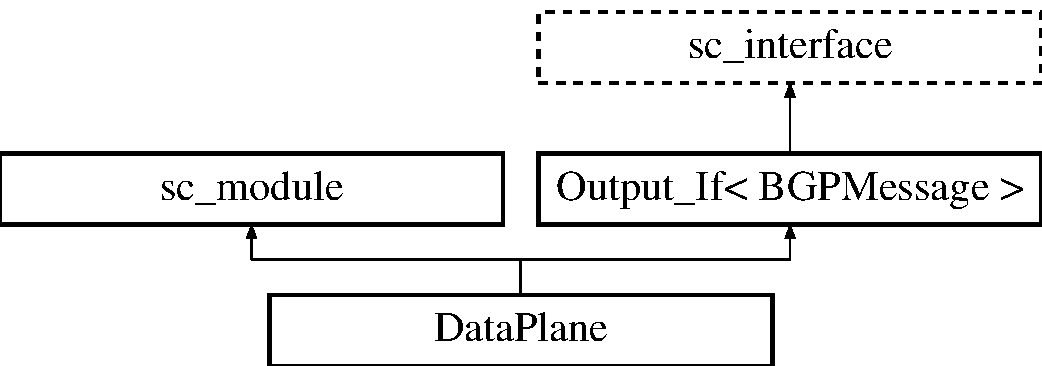
\includegraphics[height=3.000000cm]{classDataPlane}
\end{center}
\end{figure}
\subsection*{Public Member Functions}
\begin{DoxyCompactItemize}
\item 
\hyperlink{classDataPlane_a7b191716d490d613fed8a7b206fc5be2}{Data\-Plane} (sc\-\_\-module\-\_\-name p\-\_\-\-Module\-Name, \hyperlink{classControlPlaneConfig}{Control\-Plane\-Config} $\ast$const p\-\_\-\-Config)
\begin{DoxyCompactList}\small\item\em Constructor. \end{DoxyCompactList}\item 
\hypertarget{classDataPlane_a4ac1f9b5b0673d8fe0156d887c105f09}{void \hyperlink{classDataPlane_a4ac1f9b5b0673d8fe0156d887c105f09}{main} (void)}\label{classDataPlane_a4ac1f9b5b0673d8fe0156d887c105f09}

\begin{DoxyCompactList}\small\item\em This is where the B\-G\-P will sit on. Now there is only a simple example, which shows that the connections work. \end{DoxyCompactList}\item 
virtual bool \hyperlink{classDataPlane_a5ffc92484ff41f3ec1a2998ac598fe2f}{write} (\hyperlink{classBGPMessage}{B\-G\-P\-Message} \&p\-\_\-\-B\-G\-P\-Msg)
\begin{DoxyCompactList}\small\item\em Allows the session to pass B\-G\-P messages to the \hyperlink{classDataPlane}{Data\-Plane}. \end{DoxyCompactList}\item 
\hypertarget{classDataPlane_aff4c6aaf53f34f1df596985d3552600d}{void {\bfseries kill\-Data\-Plane} (void)}\label{classDataPlane_aff4c6aaf53f34f1df596985d3552600d}

\item 
\hypertarget{classDataPlane_a2b94563f9a9019377c9f80b58061f422}{void {\bfseries set\-Up} (bool p\-\_\-\-Value)}\label{classDataPlane_a2b94563f9a9019377c9f80b58061f422}

\item 
\hypertarget{classDataPlane_abdda943b9badc67126b2c6a2e5cf4133}{bool {\bfseries is\-Running} (void)}\label{classDataPlane_abdda943b9badc67126b2c6a2e5cf4133}

\item 
\hypertarget{classDataPlane_ad4a0d13e0d6d73ddbbfdd9609a4940ab}{void {\bfseries revive\-Data\-Plane} (void)}\label{classDataPlane_ad4a0d13e0d6d73ddbbfdd9609a4940ab}

\item 
\hyperlink{classDataPlane_ae73b68600990f70ac98e35c19f01fab5}{S\-C\-\_\-\-H\-A\-S\-\_\-\-P\-R\-O\-C\-E\-S\-S} (\hyperlink{classDataPlane}{Data\-Plane})
\begin{DoxyCompactList}\small\item\em Indicate the system\-C producer that this module has a process. \end{DoxyCompactList}\end{DoxyCompactItemize}
\subsection*{Data Fields}
\begin{DoxyCompactItemize}
\item 
\hypertarget{classDataPlane_ab4e32e4ecbe4ec6e448f30c4ea629ad7}{sc\-\_\-port$<$ \hyperlink{classRoutingTable__If}{Routing\-Table\-\_\-\-If} $>$ \hyperlink{classDataPlane_ab4e32e4ecbe4ec6e448f30c4ea629ad7}{port\-\_\-\-To\-Routing\-Table}}\label{classDataPlane_ab4e32e4ecbe4ec6e448f30c4ea629ad7}

\begin{DoxyCompactList}\small\item\em Export the B\-G\-P forwarding buffer's interface for Control Plane. \end{DoxyCompactList}\item 
sc\-\_\-port$<$ sc\-\_\-fifo\-\_\-out\-\_\-if\\*
$<$ \hyperlink{classBGPMessage}{B\-G\-P\-Message} $>$\\*
, 1, S\-C\-\_\-\-Z\-E\-R\-O\-\_\-\-O\-R\-\_\-\-M\-O\-R\-E\-\_\-\-B\-O\-U\-N\-D $>$ \hyperlink{classDataPlane_a3e86cb0494125c28df71313925463b61}{port\-\_\-\-To\-Control\-Plane}
\begin{DoxyCompactList}\small\item\em Output port for B\-G\-P messages. \end{DoxyCompactList}\item 
\hypertarget{classDataPlane_ab734b3906787bd215422ffa7e8ce61d5}{sc\-\_\-port$<$ sc\-\_\-fifo\-\_\-in\-\_\-if$<$ \hyperlink{classPacket}{Packet} $>$\\*
, 0, S\-C\-\_\-\-Z\-E\-R\-O\-\_\-\-O\-R\-\_\-\-M\-O\-R\-E\-\_\-\-B\-O\-U\-N\-D $>$ \hyperlink{classDataPlane_ab734b3906787bd215422ffa7e8ce61d5}{port\-\_\-\-From\-Interface}}\label{classDataPlane_ab734b3906787bd215422ffa7e8ce61d5}

\begin{DoxyCompactList}\small\item\em Neighbor writes to the receiving buffer. \end{DoxyCompactList}\item 
\hypertarget{classDataPlane_ae60298408ddadaf00f0d3405d00af6cd}{sc\-\_\-port$<$ \hyperlink{classOutput__If}{Output\-\_\-\-If}$<$ \hyperlink{classPacket}{Packet} $>$\\*
, 0, S\-C\-\_\-\-Z\-E\-R\-O\-\_\-\-O\-R\-\_\-\-M\-O\-R\-E\-\_\-\-B\-O\-U\-N\-D $>$ \hyperlink{classDataPlane_ae60298408ddadaf00f0d3405d00af6cd}{port\-\_\-\-To\-Interface}}\label{classDataPlane_ae60298408ddadaf00f0d3405d00af6cd}

\begin{DoxyCompactList}\small\item\em Forward to the neighbor. \end{DoxyCompactList}\item 
\hypertarget{classDataPlane_a2eba52aa73168c99e96cfb9b0b6ebb05}{sc\-\_\-in\-\_\-clk \hyperlink{classDataPlane_a2eba52aa73168c99e96cfb9b0b6ebb05}{port\-\_\-\-Clk}}\label{classDataPlane_a2eba52aa73168c99e96cfb9b0b6ebb05}

\begin{DoxyCompactList}\small\item\em Clock signal. \end{DoxyCompactList}\end{DoxyCompactItemize}


\subsection{Detailed Description}
Protocol Engine module. 

Definition at line 37 of file Data\-Plane.\-hpp.



\subsection{Constructor \& Destructor Documentation}
\hypertarget{classDataPlane_a7b191716d490d613fed8a7b206fc5be2}{\index{Data\-Plane@{Data\-Plane}!Data\-Plane@{Data\-Plane}}
\index{Data\-Plane@{Data\-Plane}!DataPlane@{Data\-Plane}}
\subsubsection[{Data\-Plane}]{\setlength{\rightskip}{0pt plus 5cm}Data\-Plane\-::\-Data\-Plane (
\begin{DoxyParamCaption}
\item[{sc\-\_\-module\-\_\-name}]{p\-\_\-\-Module\-Name, }
\item[{{\bf Control\-Plane\-Config} $\ast$const}]{p\-\_\-\-Config}
\end{DoxyParamCaption}
)}}\label{classDataPlane_a7b191716d490d613fed8a7b206fc5be2}


Constructor. 

Builds the router 
\begin{DoxyParams}[1]{Parameters}
\mbox{\tt in}  & {\em p\-\_\-\-Name} & The name of the module \\
\hline
\end{DoxyParams}


Definition at line 15 of file Data\-Plane.\-cpp.



\subsection{Member Function Documentation}
\hypertarget{classDataPlane_ae73b68600990f70ac98e35c19f01fab5}{\index{Data\-Plane@{Data\-Plane}!S\-C\-\_\-\-H\-A\-S\-\_\-\-P\-R\-O\-C\-E\-S\-S@{S\-C\-\_\-\-H\-A\-S\-\_\-\-P\-R\-O\-C\-E\-S\-S}}
\index{S\-C\-\_\-\-H\-A\-S\-\_\-\-P\-R\-O\-C\-E\-S\-S@{S\-C\-\_\-\-H\-A\-S\-\_\-\-P\-R\-O\-C\-E\-S\-S}!DataPlane@{Data\-Plane}}
\subsubsection[{S\-C\-\_\-\-H\-A\-S\-\_\-\-P\-R\-O\-C\-E\-S\-S}]{\setlength{\rightskip}{0pt plus 5cm}Data\-Plane\-::\-S\-C\-\_\-\-H\-A\-S\-\_\-\-P\-R\-O\-C\-E\-S\-S (
\begin{DoxyParamCaption}
\item[{{\bf Data\-Plane}}]{}
\end{DoxyParamCaption}
)}}\label{classDataPlane_ae73b68600990f70ac98e35c19f01fab5}


Indicate the system\-C producer that this module has a process. 

\begin{DoxySeeAlso}{See Also}
\href{http://www.iro.umontreal.ca/~lablasso/docs/SystemC2.0.1/html/classproducer.html}{\tt http\-://www.\-iro.\-umontreal.\-ca/$\sim$lablasso/docs/\-System\-C2.\-0.\-1/html/classproducer.\-html} 
\end{DoxySeeAlso}
\hypertarget{classDataPlane_a5ffc92484ff41f3ec1a2998ac598fe2f}{\index{Data\-Plane@{Data\-Plane}!write@{write}}
\index{write@{write}!DataPlane@{Data\-Plane}}
\subsubsection[{write}]{\setlength{\rightskip}{0pt plus 5cm}bool Data\-Plane\-::write (
\begin{DoxyParamCaption}
\item[{{\bf B\-G\-P\-Message} \&}]{}
\end{DoxyParamCaption}
)\hspace{0.3cm}{\ttfamily [virtual]}}}\label{classDataPlane_a5ffc92484ff41f3ec1a2998ac598fe2f}


Allows the session to pass B\-G\-P messages to the \hyperlink{classDataPlane}{Data\-Plane}. 

The method shall implement a mutex that takes care of the arbitraton between sessions 
\begin{DoxyParams}[1]{Parameters}
\mbox{\tt in}  & {\em \hyperlink{classBGPMessage}{B\-G\-P\-Message}} & p\-\_\-\-B\-G\-P\-Msg The B\-G\-P message to be send \\
\hline
\end{DoxyParams}
\begin{DoxyReturn}{Returns}
bool True\-: if success is valid, False\-: if not success 
\end{DoxyReturn}


Implements \hyperlink{classOutput__If_aeef0f3dff2d02e85375e914e83140602}{Output\-\_\-\-If$<$ B\-G\-P\-Message $>$}.



Definition at line 141 of file Data\-Plane.\-cpp.



\subsection{Field Documentation}
\hypertarget{classDataPlane_a3e86cb0494125c28df71313925463b61}{\index{Data\-Plane@{Data\-Plane}!port\-\_\-\-To\-Control\-Plane@{port\-\_\-\-To\-Control\-Plane}}
\index{port\-\_\-\-To\-Control\-Plane@{port\-\_\-\-To\-Control\-Plane}!DataPlane@{Data\-Plane}}
\subsubsection[{port\-\_\-\-To\-Control\-Plane}]{\setlength{\rightskip}{0pt plus 5cm}sc\-\_\-port$<$sc\-\_\-fifo\-\_\-out\-\_\-if$<${\bf B\-G\-P\-Message}$>$,1, S\-C\-\_\-\-Z\-E\-R\-O\-\_\-\-O\-R\-\_\-\-M\-O\-R\-E\-\_\-\-B\-O\-U\-N\-D$>$ Data\-Plane\-::port\-\_\-\-To\-Control\-Plane}}\label{classDataPlane_a3e86cb0494125c28df71313925463b61}


Output port for B\-G\-P messages. 

Data Plane writes all the received B\-G\-P messages into this port. The port shall be bind to the Control Plane's receiving F\-I\-F\-O 

Definition at line 57 of file Data\-Plane.\-hpp.



The documentation for this class was generated from the following files\-:\begin{DoxyCompactItemize}
\item 
/home/antipant/\-Protocol\-P\-\_\-\-Project/\hyperlink{DataPlane_8hpp}{Data\-Plane.\-hpp}\item 
/home/antipant/\-Protocol\-P\-\_\-\-Project/\hyperlink{DataPlane_8cpp}{Data\-Plane.\-cpp}\end{DoxyCompactItemize}

\hypertarget{classselectdialog_1_1Draggable}{\section{selectdialog.\-Draggable Class Reference}
\label{classselectdialog_1_1Draggable}\index{selectdialog.\-Draggable@{selectdialog.\-Draggable}}
}
Inheritance diagram for selectdialog.\-Draggable\-:\begin{figure}[H]
\begin{center}
\leavevmode
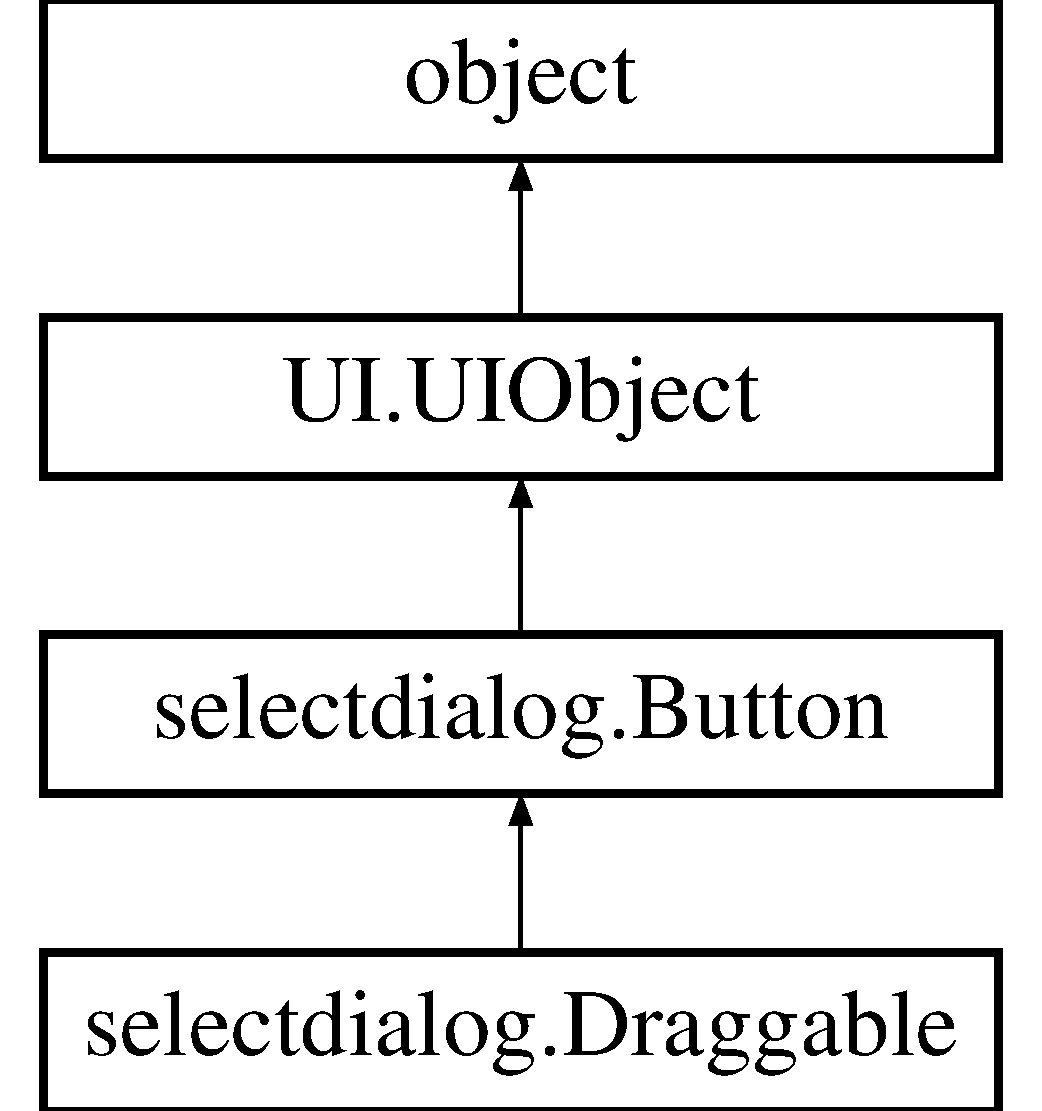
\includegraphics[height=4.000000cm]{classselectdialog_1_1Draggable}
\end{center}
\end{figure}
\subsection*{Public Member Functions}
\begin{DoxyCompactItemize}
\item 
\hypertarget{classselectdialog_1_1Draggable_a14f0264288ffaa5cf10115ffe20d6699}{def {\bfseries \-\_\-\-\_\-init\-\_\-\-\_\-}}\label{classselectdialog_1_1Draggable_a14f0264288ffaa5cf10115ffe20d6699}

\item 
\hypertarget{classselectdialog_1_1Draggable_ac6f8a0e33f1b96ba9336700a6d62c253}{def {\bfseries event}}\label{classselectdialog_1_1Draggable_ac6f8a0e33f1b96ba9336700a6d62c253}

\item 
\hypertarget{classselectdialog_1_1Draggable_ac1be90930ab822e816673a7a0dee83ff}{def {\bfseries moved}}\label{classselectdialog_1_1Draggable_ac1be90930ab822e816673a7a0dee83ff}

\end{DoxyCompactItemize}
\subsection*{Data Fields}
\begin{DoxyCompactItemize}
\item 
\hypertarget{classselectdialog_1_1Draggable_a701b7f8420093acfc4d14e13fd7ce32b}{{\bfseries rel\-\_\-pos}}\label{classselectdialog_1_1Draggable_a701b7f8420093acfc4d14e13fd7ce32b}

\end{DoxyCompactItemize}
\subsection*{Additional Inherited Members}


\subsection{Detailed Description}


Definition at line 94 of file selectdialog.\-py.



The documentation for this class was generated from the following file\-:\begin{DoxyCompactItemize}
\item 
/home/antipant/\-Protocol\-P\-\_\-\-Project/\-U\-I/selectdialog.\-py\end{DoxyCompactItemize}

\hypertarget{classselectdialog_1_1FakeGrid}{\section{selectdialog.\-Fake\-Grid Class Reference}
\label{classselectdialog_1_1FakeGrid}\index{selectdialog.\-Fake\-Grid@{selectdialog.\-Fake\-Grid}}
}
\subsection*{Public Member Functions}
\begin{DoxyCompactItemize}
\item 
\hypertarget{classselectdialog_1_1FakeGrid_a26985d20b0d787dd6a4bccdb5d2860e4}{def {\bfseries \-\_\-\-\_\-init\-\_\-\-\_\-}}\label{classselectdialog_1_1FakeGrid_a26985d20b0d787dd6a4bccdb5d2860e4}

\end{DoxyCompactItemize}
\subsection*{Data Fields}
\begin{DoxyCompactItemize}
\item 
\hypertarget{classselectdialog_1_1FakeGrid_ae40bba21382e64de5caaf2985c373127}{{\bfseries cell\-\_\-size}}\label{classselectdialog_1_1FakeGrid_ae40bba21382e64de5caaf2985c373127}

\end{DoxyCompactItemize}


\subsection{Detailed Description}


Definition at line 15 of file selectdialog.\-py.



The documentation for this class was generated from the following file\-:\begin{DoxyCompactItemize}
\item 
/home/antipant/\-Protocol\-P\-\_\-\-Project/\-U\-I/selectdialog.\-py\end{DoxyCompactItemize}

\hypertarget{classUI_1_1FuncButton}{\section{U\-I.\-Func\-Button Class Reference}
\label{classUI_1_1FuncButton}\index{U\-I.\-Func\-Button@{U\-I.\-Func\-Button}}
}
Inheritance diagram for U\-I.\-Func\-Button\-:\begin{figure}[H]
\begin{center}
\leavevmode
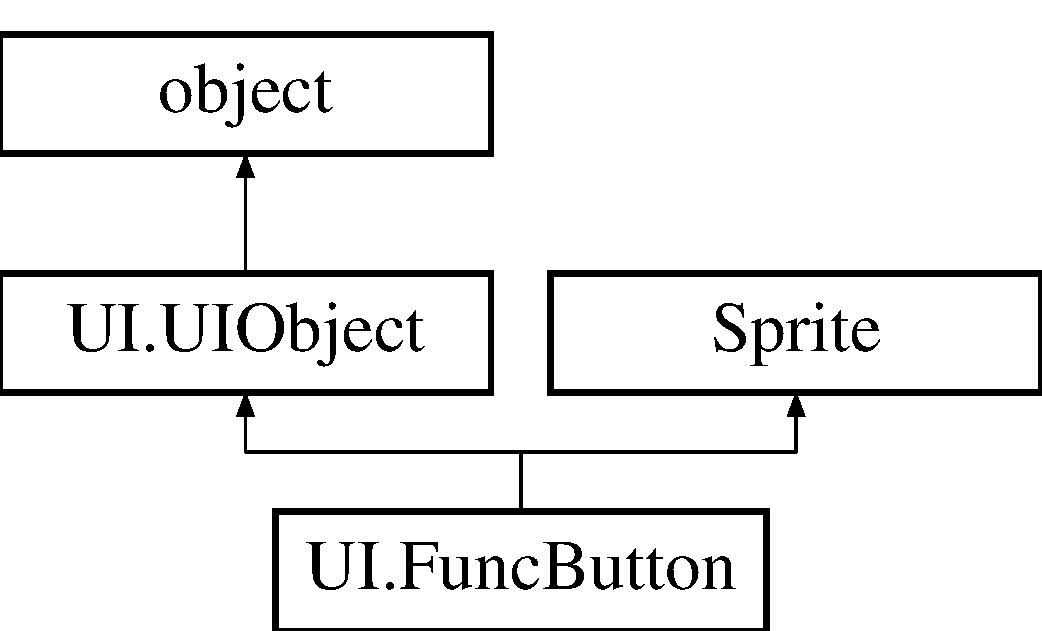
\includegraphics[height=3.000000cm]{classUI_1_1FuncButton}
\end{center}
\end{figure}
\subsection*{Public Member Functions}
\begin{DoxyCompactItemize}
\item 
\hypertarget{classUI_1_1FuncButton_a3f6f4283b4e1554d630b56d96e541b39}{def {\bfseries \-\_\-\-\_\-init\-\_\-\-\_\-}}\label{classUI_1_1FuncButton_a3f6f4283b4e1554d630b56d96e541b39}

\item 
\hypertarget{classUI_1_1FuncButton_a9345b56143c32dd9c2a11702e6bb2d9d}{def {\bfseries update}}\label{classUI_1_1FuncButton_a9345b56143c32dd9c2a11702e6bb2d9d}

\item 
\hypertarget{classUI_1_1FuncButton_aa0c69d40a1d68697c26d0ae334195524}{def {\bfseries add\-\_\-image}}\label{classUI_1_1FuncButton_aa0c69d40a1d68697c26d0ae334195524}

\item 
\hypertarget{classUI_1_1FuncButton_a641ff94293aab411710ba32b004751b4}{def {\bfseries add\-\_\-text}}\label{classUI_1_1FuncButton_a641ff94293aab411710ba32b004751b4}

\item 
\hypertarget{classUI_1_1FuncButton_af2720dacd2a29801c59de1c7c6fdfef1}{def {\bfseries show}}\label{classUI_1_1FuncButton_af2720dacd2a29801c59de1c7c6fdfef1}

\item 
\hypertarget{classUI_1_1FuncButton_a231b4e611dca8ac4332a2b3d8bb3210c}{def {\bfseries hide}}\label{classUI_1_1FuncButton_a231b4e611dca8ac4332a2b3d8bb3210c}

\item 
\hypertarget{classUI_1_1FuncButton_a6a7130ef2ef43e2976340908cba9078a}{def {\bfseries select}}\label{classUI_1_1FuncButton_a6a7130ef2ef43e2976340908cba9078a}

\item 
\hypertarget{classUI_1_1FuncButton_a816b37385493022e881a1556167f0526}{def {\bfseries unselect}}\label{classUI_1_1FuncButton_a816b37385493022e881a1556167f0526}

\item 
\hypertarget{classUI_1_1FuncButton_a2bfabd86baeed2499d11f353f1b1773a}{def {\bfseries toggle}}\label{classUI_1_1FuncButton_a2bfabd86baeed2499d11f353f1b1773a}

\item 
def \hyperlink{classUI_1_1FuncButton_a3f6efb3f6f8db074ae90309365fe2383}{add\-\_\-round\-\_\-rect}
\item 
\hypertarget{classUI_1_1FuncButton_a92024aadbac1d083161e687e73a24ae3}{def {\bfseries toggle\-\_\-visibility}}\label{classUI_1_1FuncButton_a92024aadbac1d083161e687e73a24ae3}

\end{DoxyCompactItemize}
\subsection*{Data Fields}
\begin{DoxyCompactItemize}
\item 
\hypertarget{classUI_1_1FuncButton_a7b278a0026b7cdadb0955fd0bd8c4d0e}{{\bfseries visible}}\label{classUI_1_1FuncButton_a7b278a0026b7cdadb0955fd0bd8c4d0e}

\item 
\hypertarget{classUI_1_1FuncButton_ad489c1ac26e07aa2a068eda0d1fceb18}{{\bfseries function}}\label{classUI_1_1FuncButton_ad489c1ac26e07aa2a068eda0d1fceb18}

\item 
\hypertarget{classUI_1_1FuncButton_a8f8a738b3e904b78a3cb2592a80c7627}{{\bfseries surface}}\label{classUI_1_1FuncButton_a8f8a738b3e904b78a3cb2592a80c7627}

\item 
\hypertarget{classUI_1_1FuncButton_a7bedc10ef272f38fbe1a9fad73619111}{{\bfseries fontsize}}\label{classUI_1_1FuncButton_a7bedc10ef272f38fbe1a9fad73619111}

\item 
\hypertarget{classUI_1_1FuncButton_a99bda8955797c4c1cfe72731b5366ad8}{{\bfseries bg\-\_\-color}}\label{classUI_1_1FuncButton_a99bda8955797c4c1cfe72731b5366ad8}

\item 
\hypertarget{classUI_1_1FuncButton_af782a37f536d82d7795fc402bf56a968}{{\bfseries border\-\_\-color}}\label{classUI_1_1FuncButton_af782a37f536d82d7795fc402bf56a968}

\item 
\hypertarget{classUI_1_1FuncButton_a0bd94e1a0829422013029421586630a4}{{\bfseries selected\-\_\-color}}\label{classUI_1_1FuncButton_a0bd94e1a0829422013029421586630a4}

\item 
\hypertarget{classUI_1_1FuncButton_a07ee7fa5e0dd00c5f24906780919003a}{{\bfseries images}}\label{classUI_1_1FuncButton_a07ee7fa5e0dd00c5f24906780919003a}

\item 
\hypertarget{classUI_1_1FuncButton_a740f8a00100d1e5bca7029ca477dbbc1}{{\bfseries selected}}\label{classUI_1_1FuncButton_a740f8a00100d1e5bca7029ca477dbbc1}

\item 
\hypertarget{classUI_1_1FuncButton_af3a8d528e33c2c250fd5ab7ed117e9a2}{{\bfseries static}}\label{classUI_1_1FuncButton_af3a8d528e33c2c250fd5ab7ed117e9a2}

\item 
\hypertarget{classUI_1_1FuncButton_afe0f56471d5abe428be18937db9a789e}{{\bfseries border}}\label{classUI_1_1FuncButton_afe0f56471d5abe428be18937db9a789e}

\item 
\hypertarget{classUI_1_1FuncButton_a7f10255ce8788b451910508784f5b816}{{\bfseries background}}\label{classUI_1_1FuncButton_a7f10255ce8788b451910508784f5b816}

\item 
\hypertarget{classUI_1_1FuncButton_a05d515198e47f4501530bb6b961d2699}{{\bfseries image}}\label{classUI_1_1FuncButton_a05d515198e47f4501530bb6b961d2699}

\item 
\hypertarget{classUI_1_1FuncButton_a2e0e0a2ac2490595daa1555c73ee5de6}{{\bfseries texts}}\label{classUI_1_1FuncButton_a2e0e0a2ac2490595daa1555c73ee5de6}

\end{DoxyCompactItemize}
\subsection*{Additional Inherited Members}


\subsection{Detailed Description}


Definition at line 178 of file U\-I.\-py.



\subsection{Member Function Documentation}
\hypertarget{classUI_1_1FuncButton_a3f6efb3f6f8db074ae90309365fe2383}{\index{U\-I\-::\-Func\-Button@{U\-I\-::\-Func\-Button}!add\-\_\-round\-\_\-rect@{add\-\_\-round\-\_\-rect}}
\index{add\-\_\-round\-\_\-rect@{add\-\_\-round\-\_\-rect}!UI::FuncButton@{U\-I\-::\-Func\-Button}}
\subsubsection[{add\-\_\-round\-\_\-rect}]{\setlength{\rightskip}{0pt plus 5cm}def U\-I.\-Func\-Button.\-add\-\_\-round\-\_\-rect (
\begin{DoxyParamCaption}
\item[{}]{self, }
\item[{}]{rect, }
\item[{}]{color, }
\item[{}]{radius = {\ttfamily 9}}
\end{DoxyParamCaption}
)}}\label{classUI_1_1FuncButton_a3f6efb3f6f8db074ae90309365fe2383}
\begin{DoxyVerb}AAfilledRoundedRect(surface,rect,color,radius=0.4)

surface : destination
rect    : rectangle
color   : rgb or rgba
radius  : 0 <= radius <= 1
\end{DoxyVerb}
 

Definition at line 280 of file U\-I.\-py.



The documentation for this class was generated from the following file\-:\begin{DoxyCompactItemize}
\item 
/home/antipant/\-Protocol\-P\-\_\-\-Project/\-U\-I/U\-I.\-py\end{DoxyCompactItemize}

\hypertarget{classHost}{\section{Host Class Reference}
\label{classHost}\index{Host@{Host}}
}


\hyperlink{classHost}{Host} module.  




{\ttfamily \#include $<$Host.\-hpp$>$}

Inheritance diagram for Host\-:\begin{figure}[H]
\begin{center}
\leavevmode
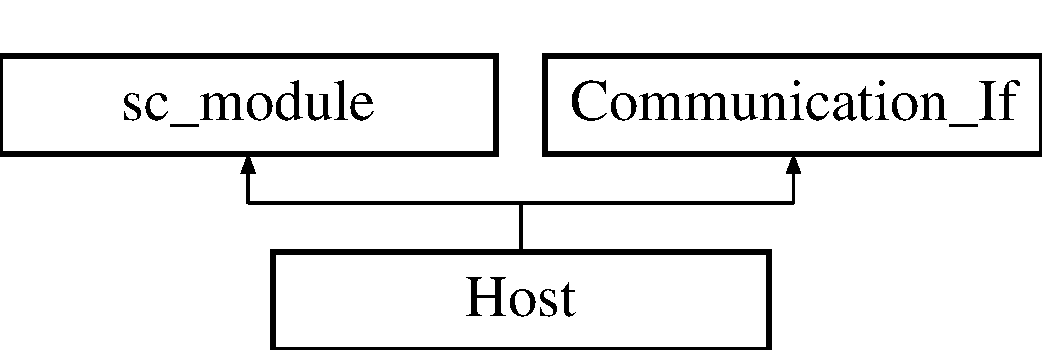
\includegraphics[height=2.000000cm]{classHost}
\end{center}
\end{figure}
\subsection*{Public Member Functions}
\begin{DoxyCompactItemize}
\item 
\hypertarget{classHost_a2b50e87ea08877ce1f618f0305cfcc30}{void {\bfseries host\-Main} (void)}\label{classHost_a2b50e87ea08877ce1f618f0305cfcc30}

\item 
\hyperlink{classHost_a8c8159669a97b7d2e7aeca227c1c0e97}{Host} (sc\-\_\-module\-\_\-name p\-\_\-\-Module\-Name, \hyperlink{classConnection}{Connection} $\ast$p\-\_\-\-Connection\-Config)
\item 
\hypertarget{classHost_abbb2fd8a913de123b33160c140d54c71}{void {\bfseries interface\-Up} (void)}\label{classHost_abbb2fd8a913de123b33160c140d54c71}

\item 
virtual bool \hyperlink{classHost_a56eb630fcf00ef1184d5df27f66a9b9e}{send\-Message} (string p\-\_\-\-Destination\-I\-P, string p\-\_\-\-Source\-I\-P, string p\-\_\-\-Payload)
\item 
virtual string \hyperlink{classHost_a4393bc6a6521e084d9f2663f8d0564bb}{rea\-Message\-Buffer} (void)
\item 
virtual void \hyperlink{classHost_aa70d91a0fd3b482f001909569b3396be}{clear\-Message\-Buffer} (void)
\item 
\hypertarget{classHost_adc2e7e8bd896b96767b11c3f3da61ec6}{{\bfseries S\-C\-\_\-\-H\-A\-S\-\_\-\-P\-R\-O\-C\-E\-S\-S} (\hyperlink{classHost}{Host})}\label{classHost_adc2e7e8bd896b96767b11c3f3da61ec6}

\end{DoxyCompactItemize}
\subsection*{Data Fields}
\begin{DoxyCompactItemize}
\item 
\hypertarget{classHost_a88a2578209c583dd5715d07a84b6c6c6}{sc\-\_\-export$<$ \hyperlink{classInterface__If}{Interface\-\_\-\-If} $>$ $\ast$$\ast$ {\bfseries export\-\_\-\-Receiving\-Interface}}\label{classHost_a88a2578209c583dd5715d07a84b6c6c6}

\item 
\hypertarget{classHost_a14ccfead574709c66f4495b3b5840957}{sc\-\_\-port$<$ \hyperlink{classInterface__If}{Interface\-\_\-\-If}, \\*
1, S\-C\-\_\-\-Z\-E\-R\-O\-\_\-\-O\-R\-\_\-\-M\-O\-R\-E\-\_\-\-B\-O\-U\-N\-D $>$ $\ast$$\ast$ {\bfseries port\-\_\-\-Forwarding\-Interface}}\label{classHost_a14ccfead574709c66f4495b3b5840957}

\end{DoxyCompactItemize}


\subsection{Detailed Description}
\hyperlink{classHost}{Host} module. 

Definition at line 38 of file Host.\-hpp.



\subsection{Constructor \& Destructor Documentation}
\hypertarget{classHost_a8c8159669a97b7d2e7aeca227c1c0e97}{\index{Host@{Host}!Host@{Host}}
\index{Host@{Host}!Host@{Host}}
\subsubsection[{Host}]{\setlength{\rightskip}{0pt plus 5cm}Host\-::\-Host (
\begin{DoxyParamCaption}
\item[{sc\-\_\-module\-\_\-name}]{p\-\_\-\-Module\-Name, }
\item[{{\bf Connection} $\ast$}]{p\-\_\-\-Connection\-Config}
\end{DoxyParamCaption}
)}}\label{classHost_a8c8159669a97b7d2e7aeca227c1c0e97}
\hyperlink{classStringTools}{String\-Tools} instance for reporting

\begin{DoxyItemize}
\item define clock period for \hyperlink{classRouter}{Router}\end{DoxyItemize}
\begin{DoxyItemize}
\item Allocate clock for the Routers using the previously allocated period \end{DoxyItemize}


Definition at line 13 of file Host.\-cpp.



\subsection{Member Function Documentation}
\hypertarget{classHost_aa70d91a0fd3b482f001909569b3396be}{\index{Host@{Host}!clear\-Message\-Buffer@{clear\-Message\-Buffer}}
\index{clear\-Message\-Buffer@{clear\-Message\-Buffer}!Host@{Host}}
\subsubsection[{clear\-Message\-Buffer}]{\setlength{\rightskip}{0pt plus 5cm}void Host\-::clear\-Message\-Buffer (
\begin{DoxyParamCaption}
\item[{void}]{}
\end{DoxyParamCaption}
)\hspace{0.3cm}{\ttfamily [virtual]}}}\label{classHost_aa70d91a0fd3b482f001909569b3396be}
\begin{DoxySeeAlso}{See Also}
\hyperlink{classCommunication__If}{Communication\-\_\-\-If} 
\end{DoxySeeAlso}


Implements \hyperlink{classCommunication__If_ad0a41ea2bebc146be6ee6db89d49486d}{Communication\-\_\-\-If}.



Definition at line 135 of file Host.\-cpp.

\hypertarget{classHost_a4393bc6a6521e084d9f2663f8d0564bb}{\index{Host@{Host}!rea\-Message\-Buffer@{rea\-Message\-Buffer}}
\index{rea\-Message\-Buffer@{rea\-Message\-Buffer}!Host@{Host}}
\subsubsection[{rea\-Message\-Buffer}]{\setlength{\rightskip}{0pt plus 5cm}string Host\-::rea\-Message\-Buffer (
\begin{DoxyParamCaption}
\item[{void}]{}
\end{DoxyParamCaption}
)\hspace{0.3cm}{\ttfamily [virtual]}}}\label{classHost_a4393bc6a6521e084d9f2663f8d0564bb}
\begin{DoxySeeAlso}{See Also}
\hyperlink{classCommunication__If}{Communication\-\_\-\-If} 
\end{DoxySeeAlso}


Implements \hyperlink{classCommunication__If_a6a6083e9f88d3bd0897ccd1c6448f9c8}{Communication\-\_\-\-If}.



Definition at line 123 of file Host.\-cpp.

\hypertarget{classHost_a56eb630fcf00ef1184d5df27f66a9b9e}{\index{Host@{Host}!send\-Message@{send\-Message}}
\index{send\-Message@{send\-Message}!Host@{Host}}
\subsubsection[{send\-Message}]{\setlength{\rightskip}{0pt plus 5cm}bool Host\-::send\-Message (
\begin{DoxyParamCaption}
\item[{string}]{p\-\_\-\-Destination\-I\-P, }
\item[{string}]{p\-\_\-\-Source\-I\-P, }
\item[{string}]{p\-\_\-\-Payload}
\end{DoxyParamCaption}
)\hspace{0.3cm}{\ttfamily [virtual]}}}\label{classHost_a56eb630fcf00ef1184d5df27f66a9b9e}
\begin{DoxySeeAlso}{See Also}
\hyperlink{classCommunication__If}{Communication\-\_\-\-If} 
\end{DoxySeeAlso}


Implements \hyperlink{classCommunication__If_ab9c0279d64e4ce15b2f54c0df6d8ee3a}{Communication\-\_\-\-If}.



Definition at line 109 of file Host.\-cpp.



The documentation for this class was generated from the following files\-:\begin{DoxyCompactItemize}
\item 
/home/antipant/\-Protocol\-P\-\_\-\-Project/\hyperlink{Host_8hpp}{Host.\-hpp}\item 
/home/antipant/\-Protocol\-P\-\_\-\-Project/\hyperlink{Host_8cpp}{Host.\-cpp}\end{DoxyCompactItemize}

\hypertarget{classeztext_1_1Input}{\section{eztext.\-Input Class Reference}
\label{classeztext_1_1Input}\index{eztext.\-Input@{eztext.\-Input}}
}
Inheritance diagram for eztext.\-Input\-:\begin{figure}[H]
\begin{center}
\leavevmode
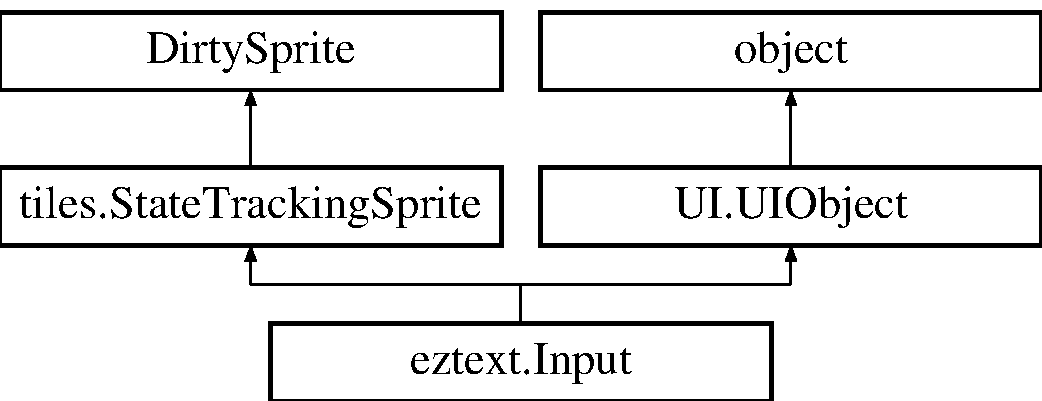
\includegraphics[height=3.000000cm]{classeztext_1_1Input}
\end{center}
\end{figure}
\subsection*{Public Member Functions}
\begin{DoxyCompactItemize}
\item 
\hypertarget{classeztext_1_1Input_a3e4f9ae6a767fd8cabe470eba31431e7}{def {\bfseries \-\_\-\-\_\-init\-\_\-\-\_\-}}\label{classeztext_1_1Input_a3e4f9ae6a767fd8cabe470eba31431e7}

\item 
\hypertarget{classeztext_1_1Input_ab8d9eb19fff57335c873adf583dae14b}{def {\bfseries update}}\label{classeztext_1_1Input_ab8d9eb19fff57335c873adf583dae14b}

\item 
\hypertarget{classeztext_1_1Input_aadb9583d8c4207e0232a55d8f44c3c22}{def {\bfseries get\-\_\-state}}\label{classeztext_1_1Input_aadb9583d8c4207e0232a55d8f44c3c22}

\item 
\hypertarget{classeztext_1_1Input_a11a8ed1c86037342050eb8a6aff76c5a}{def {\bfseries redraw}}\label{classeztext_1_1Input_a11a8ed1c86037342050eb8a6aff76c5a}

\item 
\hypertarget{classeztext_1_1Input_aaf96f3b24e705d78ddf0f31867998b49}{def {\bfseries handle\-\_\-enter}}\label{classeztext_1_1Input_aaf96f3b24e705d78ddf0f31867998b49}

\item 
\hypertarget{classeztext_1_1Input_a6ca19e326623a9fa5072c37fe501bccf}{def {\bfseries event}}\label{classeztext_1_1Input_a6ca19e326623a9fa5072c37fe501bccf}

\end{DoxyCompactItemize}
\subsection*{Data Fields}
\begin{DoxyCompactItemize}
\item 
\hypertarget{classeztext_1_1Input_a0996aabc63472676f772aea1a9f27081}{{\bfseries image}}\label{classeztext_1_1Input_a0996aabc63472676f772aea1a9f27081}

\item 
\hypertarget{classeztext_1_1Input_a306861868dafd159952b984f79bf1175}{{\bfseries font}}\label{classeztext_1_1Input_a306861868dafd159952b984f79bf1175}

\item 
\hypertarget{classeztext_1_1Input_a2c241660cdcedfd4d90ac9f73527f673}{{\bfseries color}}\label{classeztext_1_1Input_a2c241660cdcedfd4d90ac9f73527f673}

\item 
\hypertarget{classeztext_1_1Input_a13049695a51f7d3479c1e074641dbe64}{{\bfseries restricted}}\label{classeztext_1_1Input_a13049695a51f7d3479c1e074641dbe64}

\item 
\hypertarget{classeztext_1_1Input_a286491ee2241f267e0476ba3905f2734}{{\bfseries maxlength}}\label{classeztext_1_1Input_a286491ee2241f267e0476ba3905f2734}

\item 
\hypertarget{classeztext_1_1Input_a0d327652a422666c95a296fc376ad847}{{\bfseries prompt}}\label{classeztext_1_1Input_a0d327652a422666c95a296fc376ad847}

\item 
\hypertarget{classeztext_1_1Input_ac091cb15a7216b7c55b9bb9dbbe3bec9}{{\bfseries value}}\label{classeztext_1_1Input_ac091cb15a7216b7c55b9bb9dbbe3bec9}

\item 
\hypertarget{classeztext_1_1Input_a2717ee392a2a1073844eb021a7bb13b4}{{\bfseries interval}}\label{classeztext_1_1Input_a2717ee392a2a1073844eb021a7bb13b4}

\item 
\hypertarget{classeztext_1_1Input_ae1e813ab90401296c553366592280e3f}{{\bfseries count}}\label{classeztext_1_1Input_ae1e813ab90401296c553366592280e3f}

\end{DoxyCompactItemize}
\subsection*{Properties}
\begin{DoxyCompactItemize}
\item 
\hypertarget{classeztext_1_1Input_a865b332dd809f3cf4df5891e92ebabe8}{{\bfseries rect} = property(lambda self\-: pygame.\-Rect(self.\-pos, self.\-image.\-get\-\_\-size()))}\label{classeztext_1_1Input_a865b332dd809f3cf4df5891e92ebabe8}

\end{DoxyCompactItemize}


\subsection{Detailed Description}


Definition at line 11 of file eztext.\-py.



The documentation for this class was generated from the following file\-:\begin{DoxyCompactItemize}
\item 
/home/antipant/\-Protocol\-P\-\_\-\-Project/\-U\-I/eztext.\-py\end{DoxyCompactItemize}

\hypertarget{classSimulationUI_1_1Interface}{\section{Simulation\-U\-I.\-Interface Class Reference}
\label{classSimulationUI_1_1Interface}\index{Simulation\-U\-I.\-Interface@{Simulation\-U\-I.\-Interface}}
}
\subsection*{Public Member Functions}
\begin{DoxyCompactItemize}
\item 
\hypertarget{classSimulationUI_1_1Interface_a777ae8d90b540d4086db55b9c46c240b}{def {\bfseries \-\_\-\-\_\-init\-\_\-\-\_\-}}\label{classSimulationUI_1_1Interface_a777ae8d90b540d4086db55b9c46c240b}

\end{DoxyCompactItemize}
\subsection*{Data Fields}
\begin{DoxyCompactItemize}
\item 
\hypertarget{classSimulationUI_1_1Interface_a01a5b1f9a954b3c7f1d17a43bbb82c8f}{{\bfseries client}}\label{classSimulationUI_1_1Interface_a01a5b1f9a954b3c7f1d17a43bbb82c8f}

\item 
\hypertarget{classSimulationUI_1_1Interface_a2a25e845a2944548d65bb228a3a03630}{{\bfseries client\-\_\-port}}\label{classSimulationUI_1_1Interface_a2a25e845a2944548d65bb228a3a03630}

\end{DoxyCompactItemize}


\subsection{Detailed Description}


Definition at line 125 of file Simulation\-U\-I.\-py.



The documentation for this class was generated from the following file\-:\begin{DoxyCompactItemize}
\item 
/home/antipant/\-Protocol\-P\-\_\-\-Project/\-U\-I/Simulation\-U\-I.\-py\end{DoxyCompactItemize}

\hypertarget{classInterface}{\section{Interface Class Reference}
\label{classInterface}\index{Interface@{Interface}}
}


\hyperlink{classInterface}{Interface} module inside a \hyperlink{classRouter}{Router} module.  




{\ttfamily \#include $<$Interface.\-hpp$>$}

Inheritance diagram for Interface\-:\begin{figure}[H]
\begin{center}
\leavevmode
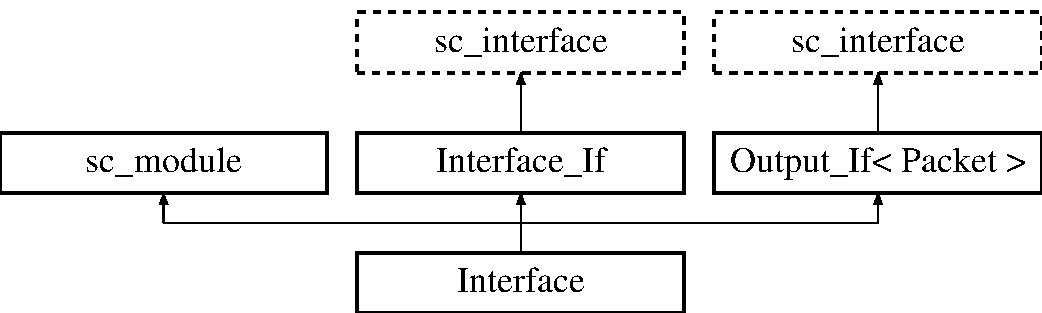
\includegraphics[height=3.000000cm]{classInterface}
\end{center}
\end{figure}
\subsection*{Public Member Functions}
\begin{DoxyCompactItemize}
\item 
\hypertarget{classInterface_a258ac26b1adb34b35eb5bd5fa7a6561c}{\hyperlink{classInterface_a258ac26b1adb34b35eb5bd5fa7a6561c}{Interface} (sc\-\_\-module\-\_\-name p\-\_\-\-Module\-Name, \hyperlink{classConnection}{Connection} $\ast$p\-\_\-\-If\-Config)}\label{classInterface_a258ac26b1adb34b35eb5bd5fa7a6561c}

\begin{DoxyCompactList}\small\item\em Network interface constructor. \end{DoxyCompactList}\item 
virtual bool \hyperlink{classInterface_aea72dc6085e96d5a69d770277738802b}{forward} (\hyperlink{classPacket}{Packet} p\-\_\-\-Packet)
\item 
\hypertarget{classInterface_ad0382d42ebfe88d2c947744a6fe139c8}{void \hyperlink{classInterface_ad0382d42ebfe88d2c947744a6fe139c8}{interface\-Main} (void)}\label{classInterface_ad0382d42ebfe88d2c947744a6fe139c8}

\begin{DoxyCompactList}\small\item\em The System\-C process of the \hyperlink{classInterface}{Interface} module. \end{DoxyCompactList}\item 
virtual void \hyperlink{classInterface_a5398e14244e698b28c060429fa5ea433}{interface\-Down} (void)
\item 
virtual bool \hyperlink{classInterface_a28a060b50df99dacb3268b4a16d980e3}{interface\-Up} (void)
\item 
virtual bool \hyperlink{classInterface_a99298b5fd1fbec6d8da500a356921652}{is\-Up} (void)
\item 
virtual void \hyperlink{classInterface_ada8771473963bc48e4ae54263a109a25}{kill\-Interface} (void)
\item 
virtual void \hyperlink{classInterface_a788362ad5da987a5113f0cf02428bd89}{reset\-Interface} (void)
\item 
virtual bool \hyperlink{classInterface_a38e700c787ec1927f1dfcbecf6d5e67e}{write} (\hyperlink{classPacket}{Packet} \&p\-\_\-\-Frame)
\begin{DoxyCompactList}\small\item\em Allows the session to pass B\-G\-P messages to the \hyperlink{classDataPlane}{Data\-Plane}. \end{DoxyCompactList}\item 
\hyperlink{classInterface_a28ace3f1bba508032ddaf36c3c304b62}{S\-C\-\_\-\-H\-A\-S\-\_\-\-P\-R\-O\-C\-E\-S\-S} (\hyperlink{classInterface}{Interface})
\begin{DoxyCompactList}\small\item\em Indicate the system\-C producer that this module has a process. \end{DoxyCompactList}\end{DoxyCompactItemize}
\subsection*{Data Fields}
\begin{DoxyCompactItemize}
\item 
\hypertarget{classInterface_a08e2ad865ffff72fac70f2df4181ba63}{sc\-\_\-in\-\_\-clk \hyperlink{classInterface_a08e2ad865ffff72fac70f2df4181ba63}{port\-\_\-\-Clk}}\label{classInterface_a08e2ad865ffff72fac70f2df4181ba63}

\begin{DoxyCompactList}\small\item\em Clock signal. \end{DoxyCompactList}\item 
\hypertarget{classInterface_ad974df84697109d6d81615c413cd9fbd}{sc\-\_\-port$<$ \hyperlink{classInterface__If}{Interface\-\_\-\-If}, \\*
1, S\-C\-\_\-\-Z\-E\-R\-O\-\_\-\-O\-R\-\_\-\-M\-O\-R\-E\-\_\-\-B\-O\-U\-N\-D $>$ {\bfseries port\-\_\-\-Output}}\label{classInterface_ad974df84697109d6d81615c413cd9fbd}

\item 
\hypertarget{classInterface_af40b9d9bf57e6ad965c4c98a6e525dd9}{sc\-\_\-export$<$ sc\-\_\-fifo\-\_\-in\-\_\-if\\*
$<$ \hyperlink{classPacket}{Packet} $>$ $>$ {\bfseries export\-\_\-\-To\-Data\-Plane}}\label{classInterface_af40b9d9bf57e6ad965c4c98a6e525dd9}

\end{DoxyCompactItemize}


\subsection{Detailed Description}
\hyperlink{classInterface}{Interface} module inside a \hyperlink{classRouter}{Router} module. 

Definition at line 39 of file Interface.\-hpp.



\subsection{Member Function Documentation}
\hypertarget{classInterface_aea72dc6085e96d5a69d770277738802b}{\index{Interface@{Interface}!forward@{forward}}
\index{forward@{forward}!Interface@{Interface}}
\subsubsection[{forward}]{\setlength{\rightskip}{0pt plus 5cm}bool Interface\-::forward (
\begin{DoxyParamCaption}
\item[{{\bf Packet}}]{p\-\_\-\-Packet}
\end{DoxyParamCaption}
)\hspace{0.3cm}{\ttfamily [virtual]}}}\label{classInterface_aea72dc6085e96d5a69d770277738802b}
\begin{DoxySeeAlso}{See Also}
\hyperlink{classInterface__If}{Interface\-\_\-\-If} 
\end{DoxySeeAlso}


Implements \hyperlink{classInterface__If_ac646e14d69d69c1e91e7054c649ad571}{Interface\-\_\-\-If}.



Definition at line 44 of file Interface.\-cpp.

\hypertarget{classInterface_a5398e14244e698b28c060429fa5ea433}{\index{Interface@{Interface}!interface\-Down@{interface\-Down}}
\index{interface\-Down@{interface\-Down}!Interface@{Interface}}
\subsubsection[{interface\-Down}]{\setlength{\rightskip}{0pt plus 5cm}void Interface\-::interface\-Down (
\begin{DoxyParamCaption}
\item[{void}]{}
\end{DoxyParamCaption}
)\hspace{0.3cm}{\ttfamily [virtual]}}}\label{classInterface_a5398e14244e698b28c060429fa5ea433}
\begin{DoxySeeAlso}{See Also}
\hyperlink{classInterface__If}{Interface\-\_\-\-If} 
\end{DoxySeeAlso}


Implements \hyperlink{classInterface__If_a9c7bc36e9daf6597ee108d398e63b990}{Interface\-\_\-\-If}.



Definition at line 73 of file Interface.\-cpp.

\hypertarget{classInterface_a28a060b50df99dacb3268b4a16d980e3}{\index{Interface@{Interface}!interface\-Up@{interface\-Up}}
\index{interface\-Up@{interface\-Up}!Interface@{Interface}}
\subsubsection[{interface\-Up}]{\setlength{\rightskip}{0pt plus 5cm}bool Interface\-::interface\-Up (
\begin{DoxyParamCaption}
\item[{void}]{}
\end{DoxyParamCaption}
)\hspace{0.3cm}{\ttfamily [virtual]}}}\label{classInterface_a28a060b50df99dacb3268b4a16d980e3}
\begin{DoxySeeAlso}{See Also}
\hyperlink{classInterface__If}{Interface\-\_\-\-If} 
\end{DoxySeeAlso}


Implements \hyperlink{classInterface__If_aa371c5e16c68e8cedcfcc7aef9dcd308}{Interface\-\_\-\-If}.



Definition at line 80 of file Interface.\-cpp.

\hypertarget{classInterface_a99298b5fd1fbec6d8da500a356921652}{\index{Interface@{Interface}!is\-Up@{is\-Up}}
\index{is\-Up@{is\-Up}!Interface@{Interface}}
\subsubsection[{is\-Up}]{\setlength{\rightskip}{0pt plus 5cm}bool Interface\-::is\-Up (
\begin{DoxyParamCaption}
\item[{void}]{}
\end{DoxyParamCaption}
)\hspace{0.3cm}{\ttfamily [virtual]}}}\label{classInterface_a99298b5fd1fbec6d8da500a356921652}
\begin{DoxySeeAlso}{See Also}
\hyperlink{classInterface__If}{Interface\-\_\-\-If} 
\end{DoxySeeAlso}


Implements \hyperlink{classInterface__If_a0a289537769bd38e98e45ff6bd8f510a}{Interface\-\_\-\-If}.



Definition at line 93 of file Interface.\-cpp.

\hypertarget{classInterface_ada8771473963bc48e4ae54263a109a25}{\index{Interface@{Interface}!kill\-Interface@{kill\-Interface}}
\index{kill\-Interface@{kill\-Interface}!Interface@{Interface}}
\subsubsection[{kill\-Interface}]{\setlength{\rightskip}{0pt plus 5cm}void Interface\-::kill\-Interface (
\begin{DoxyParamCaption}
\item[{void}]{}
\end{DoxyParamCaption}
)\hspace{0.3cm}{\ttfamily [virtual]}}}\label{classInterface_ada8771473963bc48e4ae54263a109a25}
\begin{DoxySeeAlso}{See Also}
\hyperlink{classInterface__If}{Interface\-\_\-\-If} 
\end{DoxySeeAlso}


Implements \hyperlink{classInterface__If_affd4f6a8757c1e6ce94eea6307e81b17}{Interface\-\_\-\-If}.



Definition at line 111 of file Interface.\-cpp.

\hypertarget{classInterface_a788362ad5da987a5113f0cf02428bd89}{\index{Interface@{Interface}!reset\-Interface@{reset\-Interface}}
\index{reset\-Interface@{reset\-Interface}!Interface@{Interface}}
\subsubsection[{reset\-Interface}]{\setlength{\rightskip}{0pt plus 5cm}void Interface\-::reset\-Interface (
\begin{DoxyParamCaption}
\item[{void}]{}
\end{DoxyParamCaption}
)\hspace{0.3cm}{\ttfamily [virtual]}}}\label{classInterface_a788362ad5da987a5113f0cf02428bd89}
\begin{DoxySeeAlso}{See Also}
\hyperlink{classInterface__If}{Interface\-\_\-\-If} 
\end{DoxySeeAlso}


Implements \hyperlink{classInterface__If_af97df01939e55f731963d2f82529af39}{Interface\-\_\-\-If}.



Definition at line 117 of file Interface.\-cpp.

\hypertarget{classInterface_a28ace3f1bba508032ddaf36c3c304b62}{\index{Interface@{Interface}!S\-C\-\_\-\-H\-A\-S\-\_\-\-P\-R\-O\-C\-E\-S\-S@{S\-C\-\_\-\-H\-A\-S\-\_\-\-P\-R\-O\-C\-E\-S\-S}}
\index{S\-C\-\_\-\-H\-A\-S\-\_\-\-P\-R\-O\-C\-E\-S\-S@{S\-C\-\_\-\-H\-A\-S\-\_\-\-P\-R\-O\-C\-E\-S\-S}!Interface@{Interface}}
\subsubsection[{S\-C\-\_\-\-H\-A\-S\-\_\-\-P\-R\-O\-C\-E\-S\-S}]{\setlength{\rightskip}{0pt plus 5cm}Interface\-::\-S\-C\-\_\-\-H\-A\-S\-\_\-\-P\-R\-O\-C\-E\-S\-S (
\begin{DoxyParamCaption}
\item[{{\bf Interface}}]{}
\end{DoxyParamCaption}
)}}\label{classInterface_a28ace3f1bba508032ddaf36c3c304b62}


Indicate the system\-C producer that this module has a process. 

\begin{DoxySeeAlso}{See Also}
\href{http://www.iro.umontreal.ca/~lablasso/docs/SystemC2.0.1/html/classproducer.html}{\tt http\-://www.\-iro.\-umontreal.\-ca/$\sim$lablasso/docs/\-System\-C2.\-0.\-1/html/classproducer.\-html} 
\end{DoxySeeAlso}
\hypertarget{classInterface_a38e700c787ec1927f1dfcbecf6d5e67e}{\index{Interface@{Interface}!write@{write}}
\index{write@{write}!Interface@{Interface}}
\subsubsection[{write}]{\setlength{\rightskip}{0pt plus 5cm}bool Interface\-::write (
\begin{DoxyParamCaption}
\item[{{\bf Packet} \&}]{}
\end{DoxyParamCaption}
)\hspace{0.3cm}{\ttfamily [virtual]}}}\label{classInterface_a38e700c787ec1927f1dfcbecf6d5e67e}


Allows the session to pass B\-G\-P messages to the \hyperlink{classDataPlane}{Data\-Plane}. 

The method shall implement a mutex that takes care of the arbitraton between sessions 
\begin{DoxyParams}[1]{Parameters}
\mbox{\tt in}  & {\em \hyperlink{classBGPMessage}{B\-G\-P\-Message}} & p\-\_\-\-B\-G\-P\-Msg The B\-G\-P message to be send \\
\hline
\end{DoxyParams}
\begin{DoxyReturn}{Returns}
bool True\-: if success is valid, False\-: if not success 
\end{DoxyReturn}


Implements \hyperlink{classOutput__If_aeef0f3dff2d02e85375e914e83140602}{Output\-\_\-\-If$<$ Packet $>$}.



Definition at line 61 of file Interface.\-cpp.



The documentation for this class was generated from the following files\-:\begin{DoxyCompactItemize}
\item 
/home/antipant/\-Protocol\-P\-\_\-\-Project/\hyperlink{Interface_8hpp}{Interface.\-hpp}\item 
/home/antipant/\-Protocol\-P\-\_\-\-Project/\hyperlink{Interface_8cpp}{Interface.\-cpp}\end{DoxyCompactItemize}

\hypertarget{classInterface__If}{\section{Interface\-\_\-\-If Class Reference}
\label{classInterface__If}\index{Interface\-\_\-\-If@{Interface\-\_\-\-If}}
}
Inheritance diagram for Interface\-\_\-\-If\-:\begin{figure}[H]
\begin{center}
\leavevmode
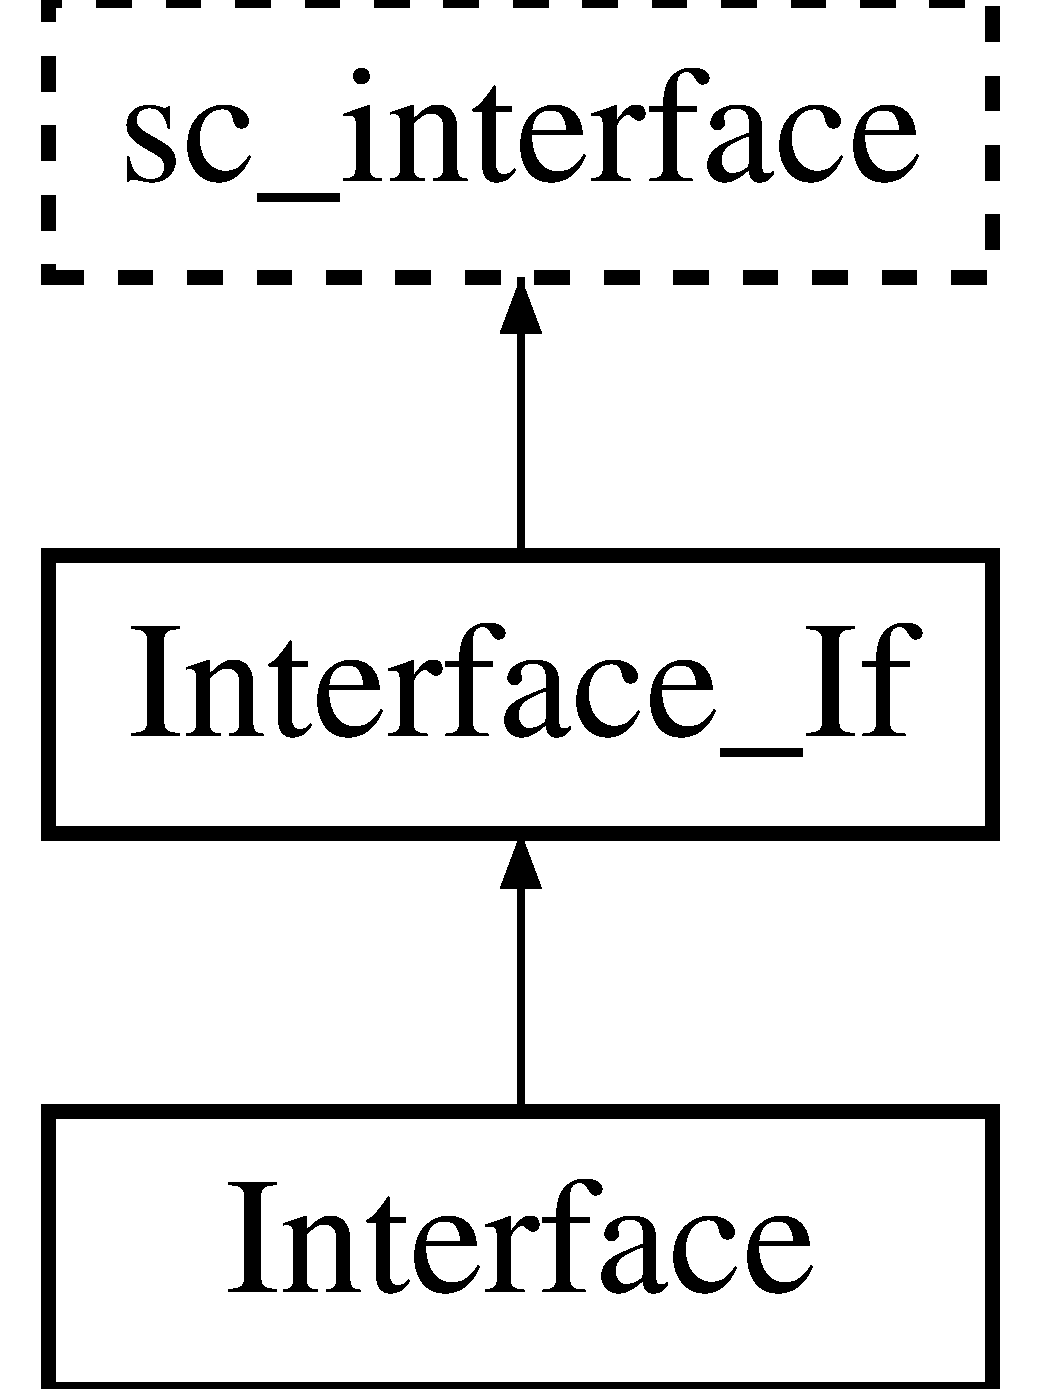
\includegraphics[height=3.000000cm]{classInterface__If}
\end{center}
\end{figure}
\subsection*{Public Member Functions}
\begin{DoxyCompactItemize}
\item 
virtual bool \hyperlink{classInterface__If_ac646e14d69d69c1e91e7054c649ad571}{forward} (\hyperlink{classPacket}{Packet} p\-\_\-\-Packet)=0
\begin{DoxyCompactList}\small\item\em Writes the p\-\_\-\-Packet to the receiving buffer of N\-I\-C that implements this I\-F. \end{DoxyCompactList}\item 
\hypertarget{classInterface__If_a9c7bc36e9daf6597ee108d398e63b990}{virtual void \hyperlink{classInterface__If_a9c7bc36e9daf6597ee108d398e63b990}{interface\-Down} (void)=0}\label{classInterface__If_a9c7bc36e9daf6597ee108d398e63b990}

\begin{DoxyCompactList}\small\item\em Sets the N\-I\-C down. \end{DoxyCompactList}\item 
\hypertarget{classInterface__If_aa371c5e16c68e8cedcfcc7aef9dcd308}{virtual bool \hyperlink{classInterface__If_aa371c5e16c68e8cedcfcc7aef9dcd308}{interface\-Up} (void)=0}\label{classInterface__If_aa371c5e16c68e8cedcfcc7aef9dcd308}

\begin{DoxyCompactList}\small\item\em Sets the N\-I\-C up. \end{DoxyCompactList}\item 
virtual bool \hyperlink{classInterface__If_a0a289537769bd38e98e45ff6bd8f510a}{is\-Up} (void)=0
\begin{DoxyCompactList}\small\item\em Checks if the N\-I\-C is up or down. \end{DoxyCompactList}\item 
\hypertarget{classInterface__If_affd4f6a8757c1e6ce94eea6307e81b17}{virtual void \hyperlink{classInterface__If_affd4f6a8757c1e6ce94eea6307e81b17}{kill\-Interface} (void)=0}\label{classInterface__If_affd4f6a8757c1e6ce94eea6307e81b17}

\begin{DoxyCompactList}\small\item\em Sets the interface down and empties the receiving and forwarding buffers. \end{DoxyCompactList}\item 
\hypertarget{classInterface__If_af97df01939e55f731963d2f82529af39}{virtual void \hyperlink{classInterface__If_af97df01939e55f731963d2f82529af39}{reset\-Interface} (void)=0}\label{classInterface__If_af97df01939e55f731963d2f82529af39}

\begin{DoxyCompactList}\small\item\em Kills the interface and reconnects it. \end{DoxyCompactList}\end{DoxyCompactItemize}


\subsection{Detailed Description}


Definition at line 30 of file Interface\-\_\-\-If.\-hpp.



\subsection{Member Function Documentation}
\hypertarget{classInterface__If_ac646e14d69d69c1e91e7054c649ad571}{\index{Interface\-\_\-\-If@{Interface\-\_\-\-If}!forward@{forward}}
\index{forward@{forward}!Interface_If@{Interface\-\_\-\-If}}
\subsubsection[{forward}]{\setlength{\rightskip}{0pt plus 5cm}bool Interface\-\_\-\-If\-::forward (
\begin{DoxyParamCaption}
\item[{{\bf Packet}}]{p\-\_\-\-Packet}
\end{DoxyParamCaption}
)\hspace{0.3cm}{\ttfamily [pure virtual]}}}\label{classInterface__If_ac646e14d69d69c1e91e7054c649ad571}


Writes the p\-\_\-\-Packet to the receiving buffer of N\-I\-C that implements this I\-F. 


\begin{DoxyParams}[1]{Parameters}
\mbox{\tt in}  & {\em \hyperlink{classPacket}{Packet}} & p\-\_\-\-Packet The network frame carring B\-G\-P msg or I\-P packet \\
\hline
\end{DoxyParams}
\begin{DoxyReturn}{Returns}
bool true\-: success false\-: N\-I\-C down or the buffer is full 
\end{DoxyReturn}


Implemented in \hyperlink{classInterface_aea72dc6085e96d5a69d770277738802b}{Interface}.

\hypertarget{classInterface__If_a0a289537769bd38e98e45ff6bd8f510a}{\index{Interface\-\_\-\-If@{Interface\-\_\-\-If}!is\-Up@{is\-Up}}
\index{is\-Up@{is\-Up}!Interface_If@{Interface\-\_\-\-If}}
\subsubsection[{is\-Up}]{\setlength{\rightskip}{0pt plus 5cm}bool Interface\-\_\-\-If\-::is\-Up (
\begin{DoxyParamCaption}
\item[{void}]{}
\end{DoxyParamCaption}
)\hspace{0.3cm}{\ttfamily [pure virtual]}}}\label{classInterface__If_a0a289537769bd38e98e45ff6bd8f510a}


Checks if the N\-I\-C is up or down. 

\begin{DoxyReturn}{Returns}
bool true\-: N\-I\-C is up -\/ false\-: N\-I\-C is down 
\end{DoxyReturn}


Implemented in \hyperlink{classInterface_a99298b5fd1fbec6d8da500a356921652}{Interface}.



The documentation for this class was generated from the following file\-:\begin{DoxyCompactItemize}
\item 
/home/antipant/\-Protocol\-P\-\_\-\-Project/\hyperlink{Interface__If_8hpp}{Interface\-\_\-\-If.\-hpp}\end{DoxyCompactItemize}

\hypertarget{classSimulationUI_1_1NameList}{\section{Simulation\-U\-I.\-Name\-List Class Reference}
\label{classSimulationUI_1_1NameList}\index{Simulation\-U\-I.\-Name\-List@{Simulation\-U\-I.\-Name\-List}}
}
Inheritance diagram for Simulation\-U\-I.\-Name\-List\-:\begin{figure}[H]
\begin{center}
\leavevmode
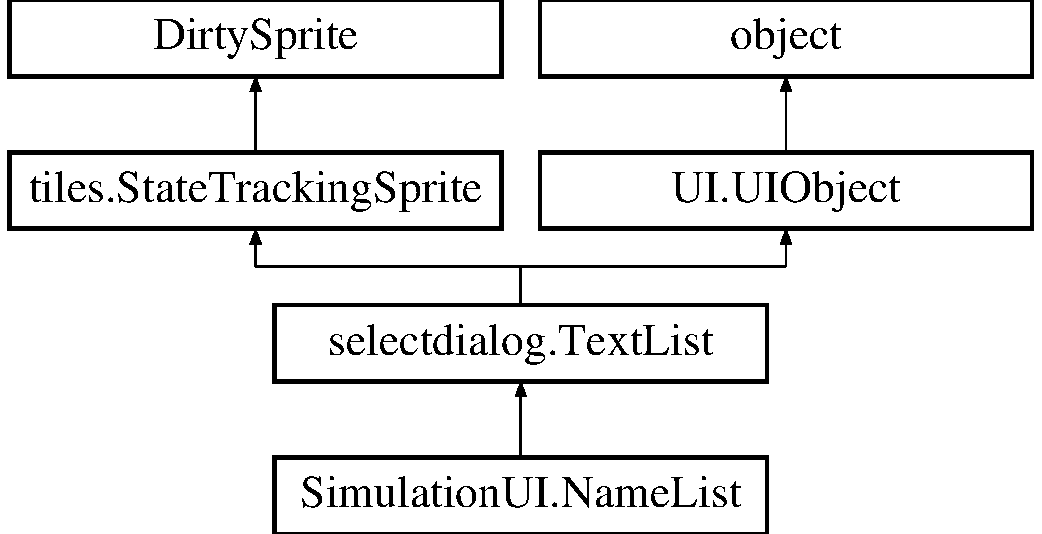
\includegraphics[height=4.000000cm]{classSimulationUI_1_1NameList}
\end{center}
\end{figure}
\subsection*{Public Member Functions}
\begin{DoxyCompactItemize}
\item 
\hypertarget{classSimulationUI_1_1NameList_a1df94c5d7deb6868ab9d422fdcef7dc6}{def {\bfseries format\-\_\-item}}\label{classSimulationUI_1_1NameList_a1df94c5d7deb6868ab9d422fdcef7dc6}

\end{DoxyCompactItemize}
\subsection*{Additional Inherited Members}


\subsection{Detailed Description}


Definition at line 25 of file Simulation\-U\-I.\-py.



The documentation for this class was generated from the following file\-:\begin{DoxyCompactItemize}
\item 
/home/antipant/\-Protocol\-P\-\_\-\-Project/\-U\-I/Simulation\-U\-I.\-py\end{DoxyCompactItemize}

\hypertarget{classOutput__If}{\section{Output\-\_\-\-If$<$ T $>$ Class Template Reference}
\label{classOutput__If}\index{Output\-\_\-\-If$<$ T $>$@{Output\-\_\-\-If$<$ T $>$}}
}
Inheritance diagram for Output\-\_\-\-If$<$ T $>$\-:\begin{figure}[H]
\begin{center}
\leavevmode
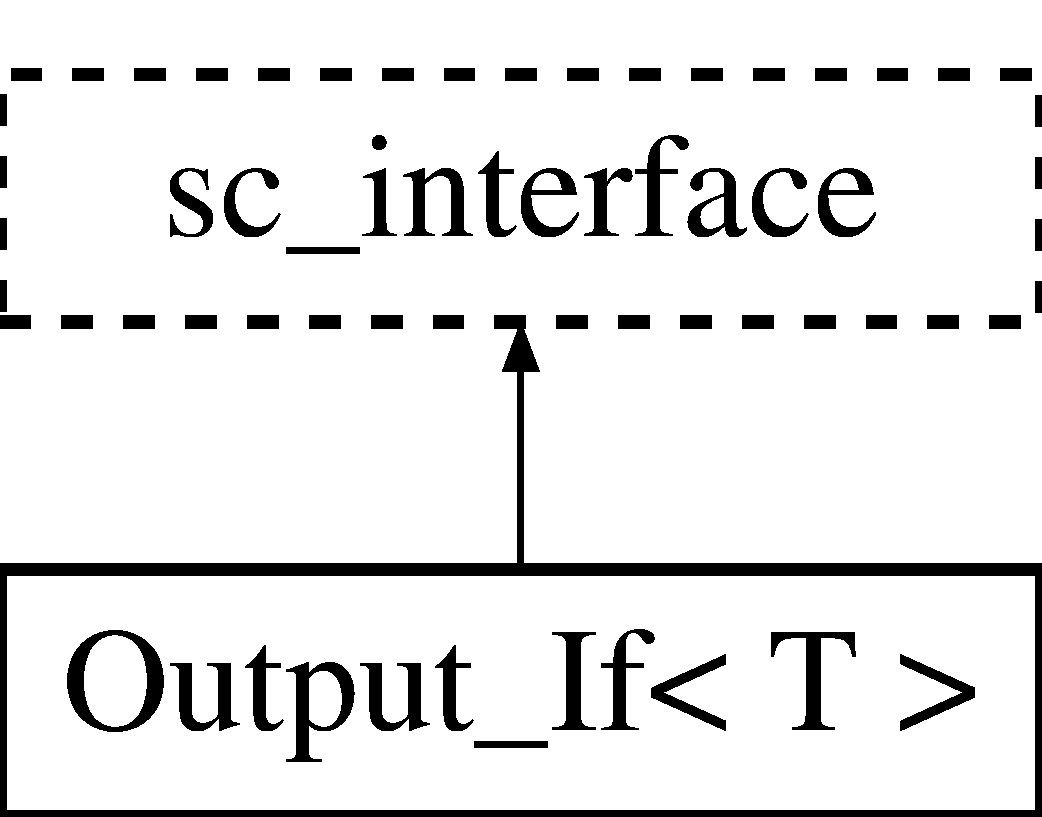
\includegraphics[height=2.000000cm]{classOutput__If}
\end{center}
\end{figure}
\subsection*{Public Member Functions}
\begin{DoxyCompactItemize}
\item 
virtual bool \hyperlink{classOutput__If_aeef0f3dff2d02e85375e914e83140602}{write} (T \&)=0
\begin{DoxyCompactList}\small\item\em Allows the session to pass B\-G\-P messages to the \hyperlink{classDataPlane}{Data\-Plane}. \end{DoxyCompactList}\end{DoxyCompactItemize}


\subsection{Detailed Description}
\subsubsection*{template$<$class T$>$class Output\-\_\-\-If$<$ T $>$}



Definition at line 29 of file Output\-\_\-\-If.\-hpp.



\subsection{Member Function Documentation}
\hypertarget{classOutput__If_aeef0f3dff2d02e85375e914e83140602}{\index{Output\-\_\-\-If@{Output\-\_\-\-If}!write@{write}}
\index{write@{write}!Output_If@{Output\-\_\-\-If}}
\subsubsection[{write}]{\setlength{\rightskip}{0pt plus 5cm}template$<$class T$>$ virtual bool {\bf Output\-\_\-\-If}$<$ T $>$\-::write (
\begin{DoxyParamCaption}
\item[{T \&}]{}
\end{DoxyParamCaption}
)\hspace{0.3cm}{\ttfamily [pure virtual]}}}\label{classOutput__If_aeef0f3dff2d02e85375e914e83140602}


Allows the session to pass B\-G\-P messages to the \hyperlink{classDataPlane}{Data\-Plane}. 

The method shall implement a mutex that takes care of the arbitraton between sessions 
\begin{DoxyParams}[1]{Parameters}
\mbox{\tt in}  & {\em \hyperlink{classBGPMessage}{B\-G\-P\-Message}} & p\-\_\-\-B\-G\-P\-Msg The B\-G\-P message to be send \\
\hline
\end{DoxyParams}
\begin{DoxyReturn}{Returns}
bool True\-: if success is valid, False\-: if not success 
\end{DoxyReturn}


Implemented in \hyperlink{classRoutingTable_ac54104a090c70c3f23799af1f30113e7}{Routing\-Table}, \hyperlink{classControlPlane_a602bc55e4d99aab6e0b38468afecdc1f}{Control\-Plane}, \hyperlink{classInterface_a38e700c787ec1927f1dfcbecf6d5e67e}{Interface}, and \hyperlink{classDataPlane_a5ffc92484ff41f3ec1a2998ac598fe2f}{Data\-Plane}.



The documentation for this class was generated from the following file\-:\begin{DoxyCompactItemize}
\item 
/home/antipant/\-Protocol\-P\-\_\-\-Project/\hyperlink{Output__If_8hpp}{Output\-\_\-\-If.\-hpp}\end{DoxyCompactItemize}

\hypertarget{classSimulationUI_1_1Packet}{\section{Simulation\-U\-I.\-Packet Class Reference}
\label{classSimulationUI_1_1Packet}\index{Simulation\-U\-I.\-Packet@{Simulation\-U\-I.\-Packet}}
}
\subsection*{Public Member Functions}
\begin{DoxyCompactItemize}
\item 
\hypertarget{classSimulationUI_1_1Packet_a244dfd6a6957079b6b8572f00ccaf333}{def {\bfseries \-\_\-\-\_\-init\-\_\-\-\_\-}}\label{classSimulationUI_1_1Packet_a244dfd6a6957079b6b8572f00ccaf333}

\item 
\hypertarget{classSimulationUI_1_1Packet_a09d64c7278685cff6d9171634018bab7}{def {\bfseries name}}\label{classSimulationUI_1_1Packet_a09d64c7278685cff6d9171634018bab7}

\end{DoxyCompactItemize}
\subsection*{Data Fields}
\begin{DoxyCompactItemize}
\item 
\hypertarget{classSimulationUI_1_1Packet_a27ca8d145d0fdcd886e724f22adfebc4}{{\bfseries header}}\label{classSimulationUI_1_1Packet_a27ca8d145d0fdcd886e724f22adfebc4}

\item 
\hypertarget{classSimulationUI_1_1Packet_a18a4813a80ec1ab6734cb4e9199b39be}{{\bfseries payload}}\label{classSimulationUI_1_1Packet_a18a4813a80ec1ab6734cb4e9199b39be}

\end{DoxyCompactItemize}


\subsection{Detailed Description}


Definition at line 117 of file Simulation\-U\-I.\-py.



The documentation for this class was generated from the following file\-:\begin{DoxyCompactItemize}
\item 
/home/antipant/\-Protocol\-P\-\_\-\-Project/\-U\-I/Simulation\-U\-I.\-py\end{DoxyCompactItemize}

\hypertarget{classPacket}{\section{Packet Class Reference}
\label{classPacket}\index{Packet@{Packet}}
}
\subsection*{Public Member Functions}
\begin{DoxyCompactItemize}
\item 
\hyperlink{classPacket_a421cbed17ae12cd3e9941f8adc788e54}{Packet} (void)
\begin{DoxyCompactList}\small\item\em Default constructor. \end{DoxyCompactList}\item 
\hyperlink{classPacket_a15a1f007e2e37e855e5533c27fc3fb7b}{$\sim$\-Packet} (void)
\begin{DoxyCompactList}\small\item\em Destructor. \end{DoxyCompactList}\item 
\hyperlink{classPacket_a7c102fea0b78944fb8391d35d643898c}{Packet} (const \hyperlink{classPacket}{Packet} \&p\-\_\-\-Packet)
\begin{DoxyCompactList}\small\item\em Constructor with member data. \end{DoxyCompactList}\item 
\hyperlink{classPacket_afb9f290d6e42db32d3888e902dc7ae50}{Packet} (\hyperlink{classBGPMessage}{B\-G\-P\-Message} \&p\-\_\-\-B\-G\-P\-Payload, int p\-\_\-\-Protocol\-Type)
\begin{DoxyCompactList}\small\item\em Constructor with member data. \end{DoxyCompactList}\item 
void \hyperlink{classPacket_a90ef09654230e093510fea3f42a88777}{set\-B\-G\-P\-Payload} (\hyperlink{classBGPMessage}{B\-G\-P\-Message} \&p\-\_\-\-B\-G\-P\-Payload)
\begin{DoxyCompactList}\small\item\em Set B\-G\-P message as payload. \end{DoxyCompactList}\item 
bool \hyperlink{classPacket_a14f94e97dfcaeaeebe7dc04b5ca71de1}{set\-Protocol\-Type} (int p\-\_\-\-Protocol\-Type)
\begin{DoxyCompactList}\small\item\em Set the upper layer protocol type. \end{DoxyCompactList}\item 
void \hyperlink{classPacket_a49433148c75138f3057e46271ec2f8fc}{set\-P\-D\-U} (const unsigned char $\ast$p\-\_\-\-P\-D\-U)
\begin{DoxyCompactList}\small\item\em Sets the P\-D\-U. \end{DoxyCompactList}\item 
void \hyperlink{classPacket_a1b85389d4a39fdc6f261f09b08041e8d}{get\-P\-D\-U} (unsigned char $\ast$p\-\_\-\-P\-D\-U)
\begin{DoxyCompactList}\small\item\em Copy P\-D\-U to the array pointed by p\-\_\-\-P\-D\-U. \end{DoxyCompactList}\item 
\hyperlink{classBGPMessage}{B\-G\-P\-Message} \& \hyperlink{classPacket_a5e573f357e5f3805041f5f0048e4e228}{get\-B\-G\-P\-Payload} (void)
\begin{DoxyCompactList}\small\item\em Get B\-G\-P Message. \end{DoxyCompactList}\item 
int \hyperlink{classPacket_a8238b0ebe88dacd1977641538cdeeba3}{get\-Protocol\-Type} (void)
\begin{DoxyCompactList}\small\item\em Get upper layer protocol type. \end{DoxyCompactList}\item 
bool \hyperlink{classPacket_a1cc5dc6d64534c637a78fdc36e9f402c}{operator==} (const \hyperlink{classPacket}{Packet} \&p\-\_\-\-Packet) const 
\begin{DoxyCompactList}\small\item\em Overload of compare operator. \end{DoxyCompactList}\item 
\hyperlink{classPacket}{Packet} \& \hyperlink{classPacket_a43e76d516ec6d5ad389e0763943f7614}{operator=} (const \hyperlink{classPacket}{Packet} \&p\-\_\-\-Packet)
\begin{DoxyCompactList}\small\item\em Overload of assign operator. \end{DoxyCompactList}\item 
\hypertarget{classPacket_a62734b071034179836086a07d6d5f35d}{string {\bfseries output\-P\-D\-U} (void)}\label{classPacket_a62734b071034179836086a07d6d5f35d}

\item 
\hypertarget{classPacket_a1a07a62259534b5764044d62551a0d9a}{void {\bfseries clear\-Packet} (void)}\label{classPacket_a1a07a62259534b5764044d62551a0d9a}

\end{DoxyCompactItemize}
\subsection*{Related Functions}
(Note that these are not member functions.) \begin{DoxyCompactItemize}
\item 
ostream \& \hyperlink{classPacket_ab2c958d68a3078ef321d8b4214f900ad}{operator$<$$<$} (ostream \&os, \hyperlink{classPacket}{Packet} const \&p\-\_\-\-Packet)
\begin{DoxyCompactList}\small\item\em Overload stream operator. \end{DoxyCompactList}\item 
void \hyperlink{classPacket_aa36ade96e213959a396cacd51c712a19}{sc\-\_\-trace} (sc\-\_\-trace\-\_\-file $\ast$p\-\_\-\-Trace\-File\-Pointer, const \hyperlink{classPacket}{Packet} \&p\-\_\-\-Packet, const string \&p\-\_\-\-Trace\-Object\-Name)
\begin{DoxyCompactList}\small\item\em Set trace file for this packet. \end{DoxyCompactList}\end{DoxyCompactItemize}


\subsection{Detailed Description}


Definition at line 38 of file Packet.\-hpp.



\subsection{Constructor \& Destructor Documentation}
\hypertarget{classPacket_a421cbed17ae12cd3e9941f8adc788e54}{\index{Packet@{Packet}!Packet@{Packet}}
\index{Packet@{Packet}!Packet@{Packet}}
\subsubsection[{Packet}]{\setlength{\rightskip}{0pt plus 5cm}Packet\-::\-Packet (
\begin{DoxyParamCaption}
\item[{void}]{}
\end{DoxyParamCaption}
)}}\label{classPacket_a421cbed17ae12cd3e9941f8adc788e54}


Default constructor. 

Initiates the packet fields to zero 

Definition at line 17 of file Packet.\-cpp.

\hypertarget{classPacket_a15a1f007e2e37e855e5533c27fc3fb7b}{\index{Packet@{Packet}!$\sim$\-Packet@{$\sim$\-Packet}}
\index{$\sim$\-Packet@{$\sim$\-Packet}!Packet@{Packet}}
\subsubsection[{$\sim$\-Packet}]{\setlength{\rightskip}{0pt plus 5cm}Packet\-::$\sim$\-Packet (
\begin{DoxyParamCaption}
\item[{void}]{}
\end{DoxyParamCaption}
)}}\label{classPacket_a15a1f007e2e37e855e5533c27fc3fb7b}


Destructor. 

Frees the member memory allocations 

Definition at line 22 of file Packet.\-cpp.

\hypertarget{classPacket_a7c102fea0b78944fb8391d35d643898c}{\index{Packet@{Packet}!Packet@{Packet}}
\index{Packet@{Packet}!Packet@{Packet}}
\subsubsection[{Packet}]{\setlength{\rightskip}{0pt plus 5cm}Packet\-::\-Packet (
\begin{DoxyParamCaption}
\item[{const {\bf Packet} \&}]{p\-\_\-\-Packet}
\end{DoxyParamCaption}
)}}\label{classPacket_a7c102fea0b78944fb8391d35d643898c}


Constructor with member data. 

Initiates the packet data and all the id fields to given values. 
\begin{DoxyParams}[1]{Parameters}
\mbox{\tt in}  & {\em const} & \hyperlink{classPacket}{Packet}\& Reference to the object to be copied into this \\
\hline
\end{DoxyParams}


Definition at line 26 of file Packet.\-cpp.

\hypertarget{classPacket_afb9f290d6e42db32d3888e902dc7ae50}{\index{Packet@{Packet}!Packet@{Packet}}
\index{Packet@{Packet}!Packet@{Packet}}
\subsubsection[{Packet}]{\setlength{\rightskip}{0pt plus 5cm}Packet\-::\-Packet (
\begin{DoxyParamCaption}
\item[{{\bf B\-G\-P\-Message} \&}]{p\-\_\-\-B\-G\-P\-Payload, }
\item[{int}]{p\-\_\-\-Protocol\-Type}
\end{DoxyParamCaption}
)}}\label{classPacket_afb9f290d6e42db32d3888e902dc7ae50}


Constructor with member data. 

Initiates the packet data and all the id fields to given values. 
\begin{DoxyParams}[1]{Parameters}
\mbox{\tt in}  & {\em B\-G\-P\-Message\&} & p\-\_\-\-B\-G\-P\-Payload Reference to the B\-G\-P payload object \\
\hline
\mbox{\tt in}  & {\em int} & p\-\_\-\-Protocol\-Type The upper layer protocol type carried in the payload \\
\hline
\end{DoxyParams}


Definition at line 33 of file Packet.\-cpp.



\subsection{Member Function Documentation}
\hypertarget{classPacket_a5e573f357e5f3805041f5f0048e4e228}{\index{Packet@{Packet}!get\-B\-G\-P\-Payload@{get\-B\-G\-P\-Payload}}
\index{get\-B\-G\-P\-Payload@{get\-B\-G\-P\-Payload}!Packet@{Packet}}
\subsubsection[{get\-B\-G\-P\-Payload}]{\setlength{\rightskip}{0pt plus 5cm}{\bf B\-G\-P\-Message} \& Packet\-::get\-B\-G\-P\-Payload (
\begin{DoxyParamCaption}
\item[{void}]{}
\end{DoxyParamCaption}
)}}\label{classPacket_a5e573f357e5f3805041f5f0048e4e228}


Get B\-G\-P Message. 

\begin{DoxyReturn}{Returns}
{\bfseries \hyperlink{classBGPMessage}{B\-G\-P\-Message}\&} Reference to B\-G\-P message object 
\end{DoxyReturn}


Definition at line 53 of file Packet.\-cpp.

\hypertarget{classPacket_a1b85389d4a39fdc6f261f09b08041e8d}{\index{Packet@{Packet}!get\-P\-D\-U@{get\-P\-D\-U}}
\index{get\-P\-D\-U@{get\-P\-D\-U}!Packet@{Packet}}
\subsubsection[{get\-P\-D\-U}]{\setlength{\rightskip}{0pt plus 5cm}void Packet\-::get\-P\-D\-U (
\begin{DoxyParamCaption}
\item[{unsigned char $\ast$}]{p\-\_\-\-P\-D\-U}
\end{DoxyParamCaption}
)}}\label{classPacket_a1b85389d4a39fdc6f261f09b08041e8d}


Copy P\-D\-U to the array pointed by p\-\_\-\-P\-D\-U. 

\begin{DoxySeeAlso}{See Also}
\hyperlink{classPacket}{Packet}
\end{DoxySeeAlso}
\begin{DoxyReturn}{Returns}
unsigned char $\ast$p\-\_\-\-P\-D\-U 
\end{DoxyReturn}


Definition at line 74 of file Packet.\-cpp.

\hypertarget{classPacket_a8238b0ebe88dacd1977641538cdeeba3}{\index{Packet@{Packet}!get\-Protocol\-Type@{get\-Protocol\-Type}}
\index{get\-Protocol\-Type@{get\-Protocol\-Type}!Packet@{Packet}}
\subsubsection[{get\-Protocol\-Type}]{\setlength{\rightskip}{0pt plus 5cm}int Packet\-::get\-Protocol\-Type (
\begin{DoxyParamCaption}
\item[{void}]{}
\end{DoxyParamCaption}
)}}\label{classPacket_a8238b0ebe88dacd1977641538cdeeba3}


Get upper layer protocol type. 

\begin{DoxyReturn}{Returns}
{\bfseries int} Indicates the upper layer protocol 
\end{DoxyReturn}


Definition at line 59 of file Packet.\-cpp.

\hypertarget{classPacket_a43e76d516ec6d5ad389e0763943f7614}{\index{Packet@{Packet}!operator=@{operator=}}
\index{operator=@{operator=}!Packet@{Packet}}
\subsubsection[{operator=}]{\setlength{\rightskip}{0pt plus 5cm}{\bf Packet} \& Packet\-::operator= (
\begin{DoxyParamCaption}
\item[{const {\bf Packet} \&}]{p\-\_\-\-Packet}
\end{DoxyParamCaption}
)}}\label{classPacket_a43e76d516ec6d5ad389e0763943f7614}


Overload of assign operator. 

Copy the data fields of given Packet-\/object to the this. Return a reference to this. 
\begin{DoxyParams}[1]{Parameters}
\mbox{\tt in}  & {\em \hyperlink{classPacket}{Packet}} & p\-\_\-\-Packet Reference to a Packet-\/object, which member values is to be assigned to the member fields of this object accordingly \\
\hline
\end{DoxyParams}
\begin{DoxyReturn}{Returns}
{\bfseries } $<$\-Packet$>$ Reference to this object 
\end{DoxyReturn}


Definition at line 95 of file Packet.\-cpp.

\hypertarget{classPacket_a1cc5dc6d64534c637a78fdc36e9f402c}{\index{Packet@{Packet}!operator==@{operator==}}
\index{operator==@{operator==}!Packet@{Packet}}
\subsubsection[{operator==}]{\setlength{\rightskip}{0pt plus 5cm}bool Packet\-::operator== (
\begin{DoxyParamCaption}
\item[{const {\bf Packet} \&}]{p\-\_\-\-Packet}
\end{DoxyParamCaption}
) const}}\label{classPacket_a1cc5dc6d64534c637a78fdc36e9f402c}


Overload of compare operator. 

Compare the data fields of this Packet-\/object to the onces in the given Packet-\/object. 
\begin{DoxyParams}[1]{Parameters}
\mbox{\tt in}  & {\em Packet\&} & p\-\_\-\-Packet Reference to a Packet-\/object to be compared with this object \\
\hline
\end{DoxyParams}
\begin{DoxyReturn}{Returns}
{\bfseries } $<$bool$>$ true if the member fields of both objects match otherwise false. 
\end{DoxyReturn}


Definition at line 85 of file Packet.\-cpp.

\hypertarget{classPacket_a90ef09654230e093510fea3f42a88777}{\index{Packet@{Packet}!set\-B\-G\-P\-Payload@{set\-B\-G\-P\-Payload}}
\index{set\-B\-G\-P\-Payload@{set\-B\-G\-P\-Payload}!Packet@{Packet}}
\subsubsection[{set\-B\-G\-P\-Payload}]{\setlength{\rightskip}{0pt plus 5cm}void Packet\-::set\-B\-G\-P\-Payload (
\begin{DoxyParamCaption}
\item[{{\bf B\-G\-P\-Message} \&}]{p\-\_\-\-B\-G\-P\-Payload}
\end{DoxyParamCaption}
)}}\label{classPacket_a90ef09654230e093510fea3f42a88777}


Set B\-G\-P message as payload. 


\begin{DoxyParams}[1]{Parameters}
\mbox{\tt in}  & {\em B\-G\-P\-Message\&} & p\-\_\-\-B\-G\-P\-Payload Reference to the B\-G\-P payload object \\
\hline
\end{DoxyParams}


Definition at line 48 of file Packet.\-cpp.

\hypertarget{classPacket_a49433148c75138f3057e46271ec2f8fc}{\index{Packet@{Packet}!set\-P\-D\-U@{set\-P\-D\-U}}
\index{set\-P\-D\-U@{set\-P\-D\-U}!Packet@{Packet}}
\subsubsection[{set\-P\-D\-U}]{\setlength{\rightskip}{0pt plus 5cm}void Packet\-::set\-P\-D\-U (
\begin{DoxyParamCaption}
\item[{const unsigned char $\ast$}]{p\-\_\-\-P\-D\-U}
\end{DoxyParamCaption}
)}}\label{classPacket_a49433148c75138f3057e46271ec2f8fc}


Sets the P\-D\-U. 


\begin{DoxyParams}[1]{Parameters}
\mbox{\tt in}  & {\em const} & unsigned char $\ast$p\-\_\-\-P\-D\-U \\
\hline
\end{DoxyParams}


Definition at line 64 of file Packet.\-cpp.

\hypertarget{classPacket_a14f94e97dfcaeaeebe7dc04b5ca71de1}{\index{Packet@{Packet}!set\-Protocol\-Type@{set\-Protocol\-Type}}
\index{set\-Protocol\-Type@{set\-Protocol\-Type}!Packet@{Packet}}
\subsubsection[{set\-Protocol\-Type}]{\setlength{\rightskip}{0pt plus 5cm}bool Packet\-::set\-Protocol\-Type (
\begin{DoxyParamCaption}
\item[{int}]{p\-\_\-\-Protocol\-Type}
\end{DoxyParamCaption}
)}}\label{classPacket_a14f94e97dfcaeaeebe7dc04b5ca71de1}


Set the upper layer protocol type. 


\begin{DoxyParams}[1]{Parameters}
\mbox{\tt in}  & {\em int} & p\-\_\-\-Protocol\-Type Value to indicate the upper layer protocol type \\
\hline
\end{DoxyParams}


Definition at line 42 of file Packet.\-cpp.



\subsection{Friends And Related Function Documentation}
\hypertarget{classPacket_ab2c958d68a3078ef321d8b4214f900ad}{\index{Packet@{Packet}!operator$<$$<$@{operator$<$$<$}}
\index{operator$<$$<$@{operator$<$$<$}!Packet@{Packet}}
\subsubsection[{operator$<$$<$}]{\setlength{\rightskip}{0pt plus 5cm}ostream\& operator$<$$<$ (
\begin{DoxyParamCaption}
\item[{ostream \&}]{os, }
\item[{{\bf Packet} const \&}]{p\-\_\-\-Packet}
\end{DoxyParamCaption}
)\hspace{0.3cm}{\ttfamily [friend]}}}\label{classPacket_ab2c958d68a3078ef321d8b4214f900ad}


Overload stream operator. 

Write data members into given output stream. 
\begin{DoxyParams}[1]{Parameters}
\mbox{\tt in}  & {\em os} & Reference to outputstream in which the member field values is to be written. \\
\hline
\mbox{\tt in}  & {\em p\-\_\-\-Packet} & Reference to Packet-\/object, which member fields is to be written into outputstream. \\
\hline
\end{DoxyParams}
\begin{DoxyReturn}{Returns}
{\bfseries } $<$ostream$>$ Reference to the outputstream containing the written values 
\end{DoxyReturn}


Definition at line 153 of file Packet.\-hpp.

\hypertarget{classPacket_aa36ade96e213959a396cacd51c712a19}{\index{Packet@{Packet}!sc\-\_\-trace@{sc\-\_\-trace}}
\index{sc\-\_\-trace@{sc\-\_\-trace}!Packet@{Packet}}
\subsubsection[{sc\-\_\-trace}]{\setlength{\rightskip}{0pt plus 5cm}void sc\-\_\-trace (
\begin{DoxyParamCaption}
\item[{sc\-\_\-trace\-\_\-file $\ast$}]{p\-\_\-\-Trace\-File\-Pointer, }
\item[{const {\bf Packet} \&}]{p\-\_\-\-Packet, }
\item[{const string \&}]{p\-\_\-\-Trace\-Object\-Name}
\end{DoxyParamCaption}
)\hspace{0.3cm}{\ttfamily [friend]}}}\label{classPacket_aa36ade96e213959a396cacd51c712a19}


Set trace file for this packet. 

All the member fields shall be traced. Allow system\-C library to access the private members of this class by declaring the function as friend 
\begin{DoxyParams}[1]{Parameters}
\mbox{\tt out}  & {\em p\-\_\-\-Trace\-File\-Pointer} & Pointer to sc\-\_\-trace\-\_\-file-\/object \\
\hline
\mbox{\tt in}  & {\em p\-\_\-\-Packet} & Reference to Packet-\/object to be traced \\
\hline
\mbox{\tt in}  & {\em p\-\_\-\-Trace\-Object\-Name} & Name of the Packet-\/object \\
\hline
\end{DoxyParams}


Definition at line 206 of file Packet.\-hpp.



The documentation for this class was generated from the following files\-:\begin{DoxyCompactItemize}
\item 
/home/antipant/\-Protocol\-P\-\_\-\-Project/\hyperlink{Packet_8hpp}{Packet.\-hpp}\item 
/home/antipant/\-Protocol\-P\-\_\-\-Project/\hyperlink{Packet_8cpp}{Packet.\-cpp}\end{DoxyCompactItemize}

\hypertarget{classPacketProcessor}{\section{Packet\-Processor Class Reference}
\label{classPacketProcessor}\index{Packet\-Processor@{Packet\-Processor}}
}


\hyperlink{classPacketProcessor}{Packet\-Processor} class.  




{\ttfamily \#include $<$Packet\-Processor.\-hpp$>$}

\subsection*{Public Member Functions}
\begin{DoxyCompactItemize}
\item 
\hypertarget{classPacketProcessor_a291d46ed0984263adeafb8468fcc73c6}{{\bfseries Packet\-Processor} (const char $\ast$p\-\_\-\-Name)}\label{classPacketProcessor_a291d46ed0984263adeafb8468fcc73c6}

\item 
\hyperlink{classPacket}{Packet} \& \hyperlink{classPacketProcessor_a2e64f01458bcc7fbe2b1fd922e1e4340}{build\-I\-P\-Packet} (string p\-\_\-\-Destination\-I\-P, string p\-\_\-\-Source\-I\-P, string p\-\_\-\-Payload)
\begin{DoxyCompactList}\small\item\em Builds an I\-P packet using the passed fields as data. \end{DoxyCompactList}\item 
string \hyperlink{classPacketProcessor_aa47781f9d17becf245930e46470261ff}{read\-I\-P\-Packet} (void)
\begin{DoxyCompactList}\small\item\em Outputs the contents of an I\-P packet. \end{DoxyCompactList}\item 
bool \hyperlink{classPacketProcessor_af9e66fdf37bfe00a3c71497dda969a56}{process\-Frame} (\hyperlink{classPacket}{Packet} \&p\-\_\-\-Packet)
\begin{DoxyCompactList}\small\item\em Validates an I\-P packet. \end{DoxyCompactList}\item 
string \hyperlink{classPacketProcessor_ac998c53191d575509fc2aa5298a1f90b}{get\-Destination} (void)
\begin{DoxyCompactList}\small\item\em Returns the destination of the processed packet. \end{DoxyCompactList}\item 
bool \hyperlink{classPacketProcessor_a631b0bd17d767c2d822cec00642402e5}{forward} (\hyperlink{classPacket}{Packet} $\ast$p\-\_\-\-Frame)
\begin{DoxyCompactList}\small\item\em copies the processed frame to the passed reference \end{DoxyCompactList}\end{DoxyCompactItemize}


\subsection{Detailed Description}
\hyperlink{classPacketProcessor}{Packet\-Processor} class. 

Performs all the tasks related to I\-P packet processing.

Allows to send, reiceve, and forward I\-P packets 

Definition at line 77 of file Packet\-Processor.\-hpp.



\subsection{Member Function Documentation}
\hypertarget{classPacketProcessor_a2e64f01458bcc7fbe2b1fd922e1e4340}{\index{Packet\-Processor@{Packet\-Processor}!build\-I\-P\-Packet@{build\-I\-P\-Packet}}
\index{build\-I\-P\-Packet@{build\-I\-P\-Packet}!PacketProcessor@{Packet\-Processor}}
\subsubsection[{build\-I\-P\-Packet}]{\setlength{\rightskip}{0pt plus 5cm}void Packet\-Processor\-::build\-I\-P\-Packet (
\begin{DoxyParamCaption}
\item[{string}]{p\-\_\-\-Destination\-I\-P, }
\item[{string}]{p\-\_\-\-Source\-I\-P, }
\item[{string}]{p\-\_\-\-Payload}
\end{DoxyParamCaption}
)}}\label{classPacketProcessor_a2e64f01458bcc7fbe2b1fd922e1e4340}


Builds an I\-P packet using the passed fields as data. 

\begin{DoxySeeAlso}{See Also}
\hyperlink{classPacketProcessor}{Packet\-Processor}
\end{DoxySeeAlso}

\begin{DoxyParams}[1]{Parameters}
\mbox{\tt in}  & {\em string} & p\-\_\-\-Destination\-I\-P \\
\hline
\mbox{\tt in}  & {\em string} & p\-\_\-\-Source\-I\-P \\
\hline
\mbox{\tt in}  & {\em string} & p\-\_\-\-Payload \\
\hline
\end{DoxyParams}
\begin{DoxyReturn}{Returns}
\hyperlink{classPacket}{Packet}\& reference to the frame that contains the built packet 
\end{DoxyReturn}


Definition at line 199 of file Packet\-Processor.\-cpp.

\hypertarget{classPacketProcessor_a631b0bd17d767c2d822cec00642402e5}{\index{Packet\-Processor@{Packet\-Processor}!forward@{forward}}
\index{forward@{forward}!PacketProcessor@{Packet\-Processor}}
\subsubsection[{forward}]{\setlength{\rightskip}{0pt plus 5cm}bool Packet\-Processor\-::forward (
\begin{DoxyParamCaption}
\item[{{\bf Packet} $\ast$}]{p\-\_\-\-Frame}
\end{DoxyParamCaption}
)}}\label{classPacketProcessor_a631b0bd17d767c2d822cec00642402e5}


copies the processed frame to the passed reference 

\begin{DoxySeeAlso}{See Also}
\hyperlink{classPacketProcessor}{Packet\-Processor}
\end{DoxySeeAlso}
decrements the T\-T\-L and recalculates the checksum using the incremental method 
\begin{DoxyParams}[1]{Parameters}
\mbox{\tt out}  & {\em Packet\&} & p\-\_\-\-Frame Reference to the object in which the processed frame should be copied \\
\hline
\end{DoxyParams}
\begin{DoxyReturn}{Returns}
bool true\-: packet is ready to be forwarded -\/ false\-: packet was dropped 
\end{DoxyReturn}


Definition at line 182 of file Packet\-Processor.\-cpp.

\hypertarget{classPacketProcessor_ac998c53191d575509fc2aa5298a1f90b}{\index{Packet\-Processor@{Packet\-Processor}!get\-Destination@{get\-Destination}}
\index{get\-Destination@{get\-Destination}!PacketProcessor@{Packet\-Processor}}
\subsubsection[{get\-Destination}]{\setlength{\rightskip}{0pt plus 5cm}string Packet\-Processor\-::get\-Destination (
\begin{DoxyParamCaption}
\item[{void}]{}
\end{DoxyParamCaption}
)}}\label{classPacketProcessor_ac998c53191d575509fc2aa5298a1f90b}


Returns the destination of the processed packet. 

\begin{DoxySeeAlso}{See Also}
\hyperlink{classPacketProcessor}{Packet\-Processor}
\end{DoxySeeAlso}
\begin{DoxyReturn}{Returns}
string\-: the destination I\-P address as string 
\end{DoxyReturn}


Definition at line 173 of file Packet\-Processor.\-cpp.

\hypertarget{classPacketProcessor_af9e66fdf37bfe00a3c71497dda969a56}{\index{Packet\-Processor@{Packet\-Processor}!process\-Frame@{process\-Frame}}
\index{process\-Frame@{process\-Frame}!PacketProcessor@{Packet\-Processor}}
\subsubsection[{process\-Frame}]{\setlength{\rightskip}{0pt plus 5cm}bool Packet\-Processor\-::process\-Frame (
\begin{DoxyParamCaption}
\item[{{\bf Packet} \&}]{p\-\_\-\-Packet}
\end{DoxyParamCaption}
)}}\label{classPacketProcessor_af9e66fdf37bfe00a3c71497dda969a56}


Validates an I\-P packet. 

\begin{DoxySeeAlso}{See Also}
\hyperlink{classPacketProcessor}{Packet\-Processor}
\end{DoxySeeAlso}
Check whether the passed packet is a valid I\-P packet. 
\begin{DoxyParams}[1]{Parameters}
\mbox{\tt in}  & {\em \hyperlink{classPacket}{Packet}} & p\-\_\-\-Packet I\-P packet to be processed \\
\hline
\end{DoxyParams}
\begin{DoxyReturn}{Returns}
bool\-: true == \hyperlink{classPacket}{Packet} is valid $|$$|$ false == \hyperlink{classPacket}{Packet} is not valid 
\end{DoxyReturn}


Definition at line 96 of file Packet\-Processor.\-cpp.

\hypertarget{classPacketProcessor_aa47781f9d17becf245930e46470261ff}{\index{Packet\-Processor@{Packet\-Processor}!read\-I\-P\-Packet@{read\-I\-P\-Packet}}
\index{read\-I\-P\-Packet@{read\-I\-P\-Packet}!PacketProcessor@{Packet\-Processor}}
\subsubsection[{read\-I\-P\-Packet}]{\setlength{\rightskip}{0pt plus 5cm}string Packet\-Processor\-::read\-I\-P\-Packet (
\begin{DoxyParamCaption}
\item[{void}]{}
\end{DoxyParamCaption}
)}}\label{classPacketProcessor_aa47781f9d17becf245930e46470261ff}


Outputs the contents of an I\-P packet. 

\begin{DoxySeeAlso}{See Also}
\hyperlink{classPacketProcessor}{Packet\-Processor}
\end{DoxySeeAlso}
The header and payload is written in the return string \begin{DoxyReturn}{Returns}
string\-: the complete I\-P packet as a string 
\end{DoxyReturn}
R\-E\-A\-D H\-E\-A\-D\-E\-R F\-I\-E\-L\-D\-S

R\-E\-A\-D P\-A\-Y\-L\-O\-A\-D 

Definition at line 26 of file Packet\-Processor.\-cpp.



The documentation for this class was generated from the following files\-:\begin{DoxyCompactItemize}
\item 
/home/antipant/\-Protocol\-P\-\_\-\-Project/\hyperlink{PacketProcessor_8hpp}{Packet\-Processor.\-hpp}\item 
/home/antipant/\-Protocol\-P\-\_\-\-Project/\hyperlink{PacketProcessor_8cpp}{Packet\-Processor.\-cpp}\end{DoxyCompactItemize}

\hypertarget{classresources_1_1Resources}{\section{resources.\-Resources Class Reference}
\label{classresources_1_1Resources}\index{resources.\-Resources@{resources.\-Resources}}
}
\subsection*{Public Member Functions}
\begin{DoxyCompactItemize}
\item 
\hypertarget{classresources_1_1Resources_a2aabcfb36634c07af118d5fe5fa2e009}{def {\bfseries \-\_\-\-\_\-init\-\_\-\-\_\-}}\label{classresources_1_1Resources_a2aabcfb36634c07af118d5fe5fa2e009}

\item 
def \hyperlink{classresources_1_1Resources_abf7e7fb914c4ba0d2095d70e341d6948}{\-\_\-\-\_\-getattr\-\_\-\-\_\-}
\item 
\hypertarget{classresources_1_1Resources_a3546aae7176af2e95c28f404f1c12ae9}{def {\bfseries load\-\_\-terrain}}\label{classresources_1_1Resources_a3546aae7176af2e95c28f404f1c12ae9}

\item 
\hypertarget{classresources_1_1Resources_a90d0bcd2f246ea1e9652e9d813ef5a55}{def {\bfseries load\-\_\-borders}}\label{classresources_1_1Resources_a90d0bcd2f246ea1e9652e9d813ef5a55}

\item 
\hypertarget{classresources_1_1Resources_a64307afecc67686d66fa0c059cd391d1}{def {\bfseries load\-\_\-overlay}}\label{classresources_1_1Resources_a64307afecc67686d66fa0c059cd391d1}

\item 
\hypertarget{classresources_1_1Resources_a9d79d7aab8f24d3db384e32a6e8c655c}{def {\bfseries load\-\_\-races}}\label{classresources_1_1Resources_a9d79d7aab8f24d3db384e32a6e8c655c}

\item 
\hypertarget{classresources_1_1Resources_aad65c15722e1d849a2c8aff4bfb1e0d9}{def {\bfseries load\-\_\-hairs}}\label{classresources_1_1Resources_aad65c15722e1d849a2c8aff4bfb1e0d9}

\item 
\hypertarget{classresources_1_1Resources_a6c87bd0afb783b66ea07b69d9a9a82bd}{def {\bfseries load\-\_\-armors}}\label{classresources_1_1Resources_a6c87bd0afb783b66ea07b69d9a9a82bd}

\item 
\hypertarget{classresources_1_1Resources_a2f1ed4db8d10e704f617e52e8f573281}{def {\bfseries load\-\_\-selections}}\label{classresources_1_1Resources_a2f1ed4db8d10e704f617e52e8f573281}

\end{DoxyCompactItemize}
\subsection*{Data Fields}
\begin{DoxyCompactItemize}
\item 
\hypertarget{classresources_1_1Resources_abd8833f9322b577fbda4e7b90fe165ed}{{\bfseries screen}}\label{classresources_1_1Resources_abd8833f9322b577fbda4e7b90fe165ed}

\item 
\hypertarget{classresources_1_1Resources_a65186e11959c922b334bf1bb6ae96dde}{{\bfseries terrain}}\label{classresources_1_1Resources_a65186e11959c922b334bf1bb6ae96dde}

\item 
\hypertarget{classresources_1_1Resources_a172bb8f56586ee89b250b8aa102b41bb}{{\bfseries borders}}\label{classresources_1_1Resources_a172bb8f56586ee89b250b8aa102b41bb}

\item 
\hypertarget{classresources_1_1Resources_a5ea106acbe434819b6f750d62f6d1954}{{\bfseries overlay}}\label{classresources_1_1Resources_a5ea106acbe434819b6f750d62f6d1954}

\item 
\hypertarget{classresources_1_1Resources_a9a2e6aa0f5a9c5ed89d4e495a9890093}{{\bfseries races}}\label{classresources_1_1Resources_a9a2e6aa0f5a9c5ed89d4e495a9890093}

\item 
\hypertarget{classresources_1_1Resources_a0111c480c85fa3f7ccd853acbd9b7649}{{\bfseries hairs}}\label{classresources_1_1Resources_a0111c480c85fa3f7ccd853acbd9b7649}

\item 
\hypertarget{classresources_1_1Resources_a1f308f7350c0ab0e727a8cd5028118de}{{\bfseries armors}}\label{classresources_1_1Resources_a1f308f7350c0ab0e727a8cd5028118de}

\item 
\hypertarget{classresources_1_1Resources_a1a6b929c37f2cd30bbc165006cae7ae7}{{\bfseries selections}}\label{classresources_1_1Resources_a1a6b929c37f2cd30bbc165006cae7ae7}

\end{DoxyCompactItemize}


\subsection{Detailed Description}


Definition at line 7 of file resources.\-py.



\subsection{Member Function Documentation}
\hypertarget{classresources_1_1Resources_abf7e7fb914c4ba0d2095d70e341d6948}{\index{resources\-::\-Resources@{resources\-::\-Resources}!\-\_\-\-\_\-getattr\-\_\-\-\_\-@{\-\_\-\-\_\-getattr\-\_\-\-\_\-}}
\index{\-\_\-\-\_\-getattr\-\_\-\-\_\-@{\-\_\-\-\_\-getattr\-\_\-\-\_\-}!resources::Resources@{resources\-::\-Resources}}
\subsubsection[{\-\_\-\-\_\-getattr\-\_\-\-\_\-}]{\setlength{\rightskip}{0pt plus 5cm}def resources.\-Resources.\-\_\-\-\_\-getattr\-\_\-\-\_\- (
\begin{DoxyParamCaption}
\item[{}]{self, }
\item[{}]{name}
\end{DoxyParamCaption}
)}}\label{classresources_1_1Resources_abf7e7fb914c4ba0d2095d70e341d6948}
\begin{DoxyVerb}Autoload resources as they are accessed\end{DoxyVerb}
 

Definition at line 11 of file resources.\-py.



The documentation for this class was generated from the following file\-:\begin{DoxyCompactItemize}
\item 
/home/antipant/\-Protocol\-P\-\_\-\-Project/\-U\-I/resources.\-py\end{DoxyCompactItemize}

\hypertarget{classSimulationUI_1_1Route}{\section{Simulation\-U\-I.\-Route Class Reference}
\label{classSimulationUI_1_1Route}\index{Simulation\-U\-I.\-Route@{Simulation\-U\-I.\-Route}}
}
\subsection*{Public Member Functions}
\begin{DoxyCompactItemize}
\item 
\hypertarget{classSimulationUI_1_1Route_a9e161b3cd0875cea5c62b4b4af851ce8}{def {\bfseries \-\_\-\-\_\-init\-\_\-\-\_\-}}\label{classSimulationUI_1_1Route_a9e161b3cd0875cea5c62b4b4af851ce8}

\item 
\hypertarget{classSimulationUI_1_1Route_aeb39cfa548a2a6112041d2930874b593}{def {\bfseries name}}\label{classSimulationUI_1_1Route_aeb39cfa548a2a6112041d2930874b593}

\end{DoxyCompactItemize}
\subsection*{Data Fields}
\begin{DoxyCompactItemize}
\item 
\hypertarget{classSimulationUI_1_1Route_ad7c3293c79fb9a17a289a45661595c32}{{\bfseries target\-\_\-as}}\label{classSimulationUI_1_1Route_ad7c3293c79fb9a17a289a45661595c32}

\item 
\hypertarget{classSimulationUI_1_1Route_ac4542ce5b48705d71a694d74544d679e}{{\bfseries prefix}}\label{classSimulationUI_1_1Route_ac4542ce5b48705d71a694d74544d679e}

\item 
\hypertarget{classSimulationUI_1_1Route_af2476e912be995188b4c5420d5b9ef2f}{{\bfseries path}}\label{classSimulationUI_1_1Route_af2476e912be995188b4c5420d5b9ef2f}

\end{DoxyCompactItemize}


\subsection{Detailed Description}


Definition at line 130 of file Simulation\-U\-I.\-py.



The documentation for this class was generated from the following file\-:\begin{DoxyCompactItemize}
\item 
/home/antipant/\-Protocol\-P\-\_\-\-Project/\-U\-I/Simulation\-U\-I.\-py\end{DoxyCompactItemize}

\hypertarget{classRouter}{\section{Router Class Reference}
\label{classRouter}\index{Router@{Router}}
}


\hyperlink{classRouter}{Router} module.  




{\ttfamily \#include $<$Router.\-hpp$>$}

Inheritance diagram for Router\-:\begin{figure}[H]
\begin{center}
\leavevmode
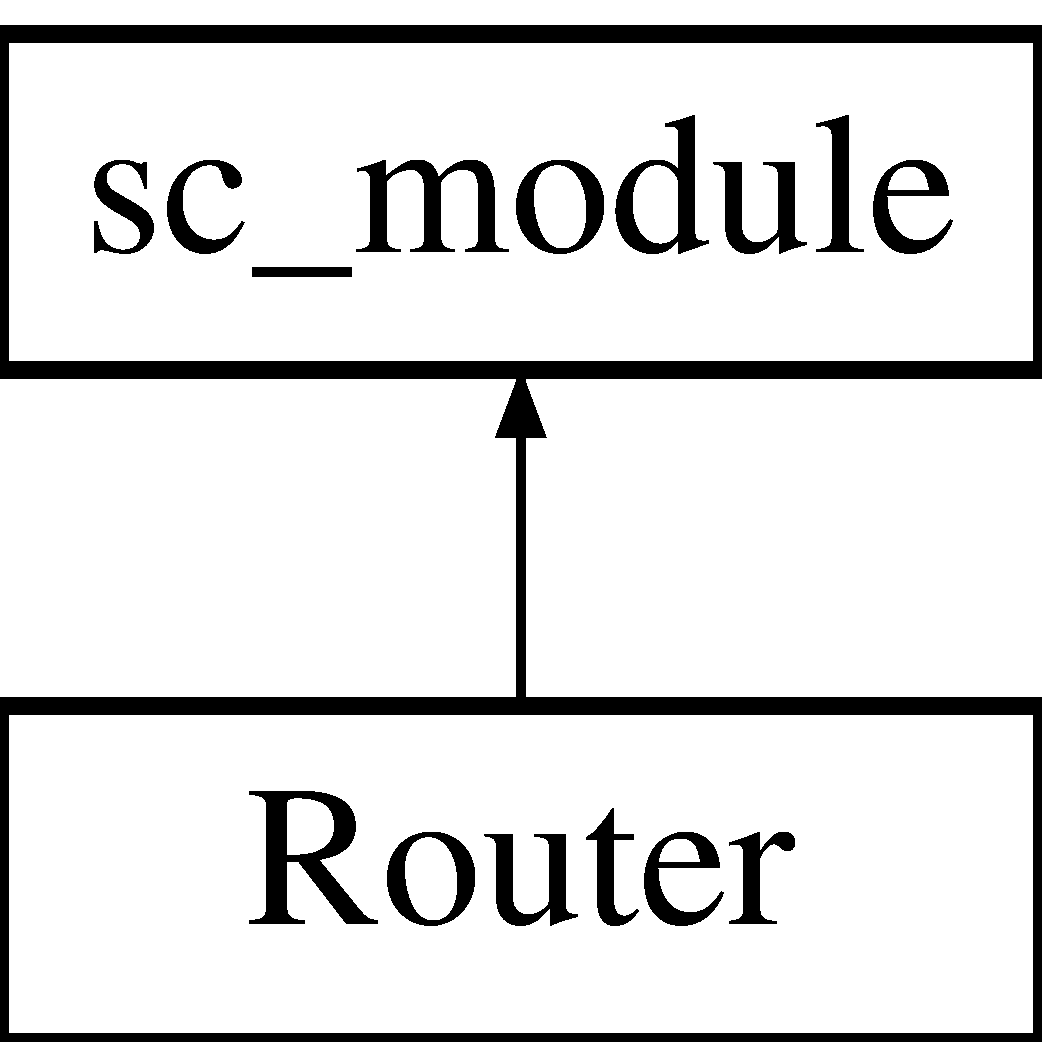
\includegraphics[height=2.000000cm]{classRouter}
\end{center}
\end{figure}
\subsection*{Public Member Functions}
\begin{DoxyCompactItemize}
\item 
\hyperlink{classRouter_a9f15cc9e3d8349adfac38175ae9ebd64}{Router} (sc\-\_\-module\-\_\-name p\-\_\-\-Module\-Name, \hyperlink{classRouterConfig}{Router\-Config} $\ast$const p\-\_\-\-Router\-Configuration)
\begin{DoxyCompactList}\small\item\em Constructor. \end{DoxyCompactList}\item 
void \hyperlink{classRouter_a31324e31f2c02c9998afdbeeb9e34c08}{interface\-Up} (int p\-\_\-\-Interface\-Id)
\begin{DoxyCompactList}\small\item\em Sets the given interface up. \end{DoxyCompactList}\item 
void \hyperlink{classRouter_ae9c407addfa058a197d005ccc600b3e1}{interface\-Down} (int p\-\_\-\-Interface\-Id)
\begin{DoxyCompactList}\small\item\em Sets the given interface down. \end{DoxyCompactList}\item 
bool \hyperlink{classRouter_aff2f6f94c5d27c2b3eb6751475f82231}{interface\-Is\-Up} (int p\-\_\-\-Interface\-Id)
\begin{DoxyCompactList}\small\item\em Checks whether the given interface is up or not. \end{DoxyCompactList}\item 
bool \hyperlink{classRouter_a6d9dd4f4e1abc82e92ab082da52f2abd}{connect\-Interface} (\hyperlink{classRouter}{Router} $\ast$p\-\_\-\-Target\-Router, int p\-\_\-\-Local\-Interface, int p\-\_\-\-Target\-Interface)
\begin{DoxyCompactList}\small\item\em Connects the given interface of this router to the given interface of the given router. \end{DoxyCompactList}\item 
\hypertarget{classRouter_aad50fac7b3c4de2e91c60a07a2bc5928}{bool {\bfseries connect\-Interface} (\hyperlink{classHost}{Host} $\ast$p\-\_\-\-Target\-Host, int p\-\_\-\-Local\-Interface)}\label{classRouter_aad50fac7b3c4de2e91c60a07a2bc5928}

\item 
\hypertarget{classRouter_aeb1245557614ed4a64e2985cec097d5b}{void \hyperlink{classRouter_aeb1245557614ed4a64e2985cec097d5b}{kill\-Router} (void)}\label{classRouter_aeb1245557614ed4a64e2985cec097d5b}

\begin{DoxyCompactList}\small\item\em Sets all the interfaces of this router down, clears all the buffers, clears all B\-G\-P sessions, resets the B\-G\-P. \end{DoxyCompactList}\item 
\hypertarget{classRouter_a9999f57baf9d5256ec69dcac3ca353f2}{void {\bfseries reset\-Router} (void)}\label{classRouter_a9999f57baf9d5256ec69dcac3ca353f2}

\item 
\hypertarget{classRouter_aa319f6fa86518d738e88dbbc7f6c07ea}{void {\bfseries revive\-Router} (void)}\label{classRouter_aa319f6fa86518d738e88dbbc7f6c07ea}

\item 
void \hyperlink{classRouter_a40a957094f6af8be1b3e8d0aae7d4c46}{kill\-Interface} (int p\-\_\-\-Interface\-Id)
\begin{DoxyCompactList}\small\item\em kills the given interface \end{DoxyCompactList}\item 
void \hyperlink{classRouter_a32df24b6aabbca7eb5bceb6e114bec2b}{reset\-Interface} (int p\-\_\-\-Interface\-Id)
\begin{DoxyCompactList}\small\item\em reset the given interface \end{DoxyCompactList}\item 
void \hyperlink{classRouter_a77e20f60d40305bcc245724c0e1224d3}{disconnect\-Interface} (int p\-\_\-\-Interface\-Id)
\begin{DoxyCompactList}\small\item\em disconnects the given interface \end{DoxyCompactList}\item 
\hypertarget{classRouter_ae8dd59d5faf07e8b95b912acba63910d}{void {\bfseries connect\-Interface} (int p\-\_\-\-Interface\-Id)}\label{classRouter_ae8dd59d5faf07e8b95b912acba63910d}

\item 
\hypertarget{classRouter_aaa7a2f17b0ab3f316c8fcf4340d23cb9}{void \hyperlink{classRouter_aaa7a2f17b0ab3f316c8fcf4340d23cb9}{disconnect\-Interfaces} (void)}\label{classRouter_aaa7a2f17b0ab3f316c8fcf4340d23cb9}

\begin{DoxyCompactList}\small\item\em disconnects all the interfaces \end{DoxyCompactList}\item 
\hypertarget{classRouter_aaafae7a061d23b34668e4bcd2d6c09fa}{void {\bfseries connect\-Interfaces} (void)}\label{classRouter_aaafae7a061d23b34668e4bcd2d6c09fa}

\item 
\hypertarget{classRouter_a88a647aff2e6e2f27c1a905a3e514b08}{string \hyperlink{classRouter_a88a647aff2e6e2f27c1a905a3e514b08}{get\-Routing\-Table} (void)}\label{classRouter_a88a647aff2e6e2f27c1a905a3e514b08}

\begin{DoxyCompactList}\small\item\em get the routing table as a string \end{DoxyCompactList}\item 
\hypertarget{classRouter_a93327fb1efd8d25e2f71c3761d9f77e9}{string \hyperlink{classRouter_a93327fb1efd8d25e2f71c3761d9f77e9}{get\-Raw\-Routing\-Table} (void)}\label{classRouter_a93327fb1efd8d25e2f71c3761d9f77e9}

\begin{DoxyCompactList}\small\item\em get the raw routing table as a string \end{DoxyCompactList}\item 
\hypertarget{classRouter_a8d4f91c2cf123344658ecce29c48fc03}{void \hyperlink{classRouter_a8d4f91c2cf123344658ecce29c48fc03}{set\-Preferred\-A\-S} (int p\-\_\-\-A\-S, int p\-\_\-pref\-\_\-value)}\label{classRouter_a8d4f91c2cf123344658ecce29c48fc03}

\begin{DoxyCompactList}\small\item\em give preference value for A\-S \end{DoxyCompactList}\item 
\hypertarget{classRouter_a0099c9da9f1a15f2b09b802a821fa28a}{void \hyperlink{classRouter_a0099c9da9f1a15f2b09b802a821fa28a}{remove\-Local\-Pref} (int p\-\_\-\-A\-S)}\label{classRouter_a0099c9da9f1a15f2b09b802a821fa28a}

\begin{DoxyCompactList}\small\item\em remove given A\-S from the list of preferred A\-Ses \end{DoxyCompactList}\end{DoxyCompactItemize}
\subsection*{Data Fields}
\begin{DoxyCompactItemize}
\item 
\hypertarget{classRouter_ad129f204d0b4465cd04c32d49064f9bc}{sc\-\_\-export$<$ \hyperlink{classInterface__If}{Interface\-\_\-\-If} $>$ $\ast$$\ast$ {\bfseries export\-\_\-\-Receiving\-Interface}}\label{classRouter_ad129f204d0b4465cd04c32d49064f9bc}

\item 
\hypertarget{classRouter_a4c1aadfe9e469ea46f77cdb1a652ba3d}{sc\-\_\-port$<$ \hyperlink{classInterface__If}{Interface\-\_\-\-If}, \\*
1, S\-C\-\_\-\-Z\-E\-R\-O\-\_\-\-O\-R\-\_\-\-M\-O\-R\-E\-\_\-\-B\-O\-U\-N\-D $>$ $\ast$$\ast$ {\bfseries port\-\_\-\-Forwarding\-Interface}}\label{classRouter_a4c1aadfe9e469ea46f77cdb1a652ba3d}

\end{DoxyCompactItemize}


\subsection{Detailed Description}
\hyperlink{classRouter}{Router} module. 

The module combines \hyperlink{classDataPlane}{Data\-Plane}, \hyperlink{classControlPlane}{Control\-Plane}, \hyperlink{classRoutingTable}{Routing\-Table}, and \hyperlink{classInterface}{Interface} modules to a single \hyperlink{classRouter}{Router} module. In addition, the router module offer a set of methods to extract data from the submodules. The router builds the submodules and binds their ports. The number of interfaces in the router is defined in the configuration object that is passed to the router as constructor argument. 

Definition at line 40 of file Router.\-hpp.



\subsection{Constructor \& Destructor Documentation}
\hypertarget{classRouter_a9f15cc9e3d8349adfac38175ae9ebd64}{\index{Router@{Router}!Router@{Router}}
\index{Router@{Router}!Router@{Router}}
\subsubsection[{Router}]{\setlength{\rightskip}{0pt plus 5cm}Router\-::\-Router (
\begin{DoxyParamCaption}
\item[{sc\-\_\-module\-\_\-name}]{p\-\_\-\-Module\-Name, }
\item[{{\bf Router\-Config} $\ast$const}]{p\-\_\-\-Router\-Configuration}
\end{DoxyParamCaption}
)}}\label{classRouter_a9f15cc9e3d8349adfac38175ae9ebd64}


Constructor. 

Builds the router 
\begin{DoxyParams}[1]{Parameters}
\mbox{\tt in}  & {\em p\-\_\-\-Name} & The name of the module \\
\hline
\end{DoxyParams}
\hyperlink{classStringTools}{String\-Tools} instance for reporting

\begin{DoxyItemize}
\item define clock period for \hyperlink{classRouter}{Router}\end{DoxyItemize}
\begin{DoxyItemize}
\item Allocate clock for the Routers using the previously allocated period \end{DoxyItemize}


Definition at line 13 of file Router.\-cpp.



\subsection{Member Function Documentation}
\hypertarget{classRouter_a6d9dd4f4e1abc82e92ab082da52f2abd}{\index{Router@{Router}!connect\-Interface@{connect\-Interface}}
\index{connect\-Interface@{connect\-Interface}!Router@{Router}}
\subsubsection[{connect\-Interface}]{\setlength{\rightskip}{0pt plus 5cm}bool Router\-::connect\-Interface (
\begin{DoxyParamCaption}
\item[{{\bf Router} $\ast$}]{p\-\_\-\-Target\-Router, }
\item[{int}]{p\-\_\-\-Local\-Interface, }
\item[{int}]{p\-\_\-\-Target\-Interface}
\end{DoxyParamCaption}
)}}\label{classRouter_a6d9dd4f4e1abc82e92ab082da52f2abd}


Connects the given interface of this router to the given interface of the given router. 


\begin{DoxyParams}[1]{Parameters}
\mbox{\tt in}  & {\em \hyperlink{classRouter}{Router}} & $\ast$p\-\_\-\-Target\-Router \\
\hline
\mbox{\tt in}  & {\em int} & p\-\_\-\-Local\-Interface \\
\hline
\mbox{\tt in}  & {\em int} & p\-\_\-\-Target\-Interface \\
\hline
\end{DoxyParams}
\begin{DoxyReturn}{Returns}
bool true\-: if success or alredy connected -\/ false\-: if one of the interfaces is conected and the other is not 
\end{DoxyReturn}


Definition at line 172 of file Router.\-cpp.

\hypertarget{classRouter_a77e20f60d40305bcc245724c0e1224d3}{\index{Router@{Router}!disconnect\-Interface@{disconnect\-Interface}}
\index{disconnect\-Interface@{disconnect\-Interface}!Router@{Router}}
\subsubsection[{disconnect\-Interface}]{\setlength{\rightskip}{0pt plus 5cm}void Router\-::disconnect\-Interface (
\begin{DoxyParamCaption}
\item[{int}]{p\-\_\-\-Interface\-Id}
\end{DoxyParamCaption}
)}}\label{classRouter_a77e20f60d40305bcc245724c0e1224d3}


disconnects the given interface 

connects all the interfaces

connects the given interface


\begin{DoxyParams}[1]{Parameters}
\mbox{\tt in}  & {\em int} & p\-\_\-\-Interface\-Id The id of the interface to be disconnected\\
\hline
\mbox{\tt in}  & {\em int} & p\-\_\-\-Interface\-Id The id of the interface to be connected \\
\hline
\end{DoxyParams}


Definition at line 263 of file Router.\-cpp.

\hypertarget{classRouter_ae9c407addfa058a197d005ccc600b3e1}{\index{Router@{Router}!interface\-Down@{interface\-Down}}
\index{interface\-Down@{interface\-Down}!Router@{Router}}
\subsubsection[{interface\-Down}]{\setlength{\rightskip}{0pt plus 5cm}void Router\-::interface\-Down (
\begin{DoxyParamCaption}
\item[{int}]{p\-\_\-\-Interface\-Id}
\end{DoxyParamCaption}
)}}\label{classRouter_ae9c407addfa058a197d005ccc600b3e1}


Sets the given interface down. 


\begin{DoxyParams}[1]{Parameters}
\mbox{\tt in}  & {\em int} & p\-\_\-\-Number\-Of\-Routers The id of the interface to be set down \\
\hline
\end{DoxyParams}


Definition at line 146 of file Router.\-cpp.

\hypertarget{classRouter_aff2f6f94c5d27c2b3eb6751475f82231}{\index{Router@{Router}!interface\-Is\-Up@{interface\-Is\-Up}}
\index{interface\-Is\-Up@{interface\-Is\-Up}!Router@{Router}}
\subsubsection[{interface\-Is\-Up}]{\setlength{\rightskip}{0pt plus 5cm}bool Router\-::interface\-Is\-Up (
\begin{DoxyParamCaption}
\item[{int}]{p\-\_\-\-Interface\-Id}
\end{DoxyParamCaption}
)}}\label{classRouter_aff2f6f94c5d27c2b3eb6751475f82231}


Checks whether the given interface is up or not. 


\begin{DoxyParams}[1]{Parameters}
\mbox{\tt in}  & {\em int} & p\-\_\-\-Interface\-Id The id of the interface to be set checked \\
\hline
\end{DoxyParams}
\begin{DoxyReturn}{Returns}
bool true\-: if up -\/ false\-: if down 
\end{DoxyReturn}


Definition at line 154 of file Router.\-cpp.

\hypertarget{classRouter_a31324e31f2c02c9998afdbeeb9e34c08}{\index{Router@{Router}!interface\-Up@{interface\-Up}}
\index{interface\-Up@{interface\-Up}!Router@{Router}}
\subsubsection[{interface\-Up}]{\setlength{\rightskip}{0pt plus 5cm}void Router\-::interface\-Up (
\begin{DoxyParamCaption}
\item[{int}]{p\-\_\-\-Interface\-Id}
\end{DoxyParamCaption}
)}}\label{classRouter_a31324e31f2c02c9998afdbeeb9e34c08}


Sets the given interface up. 


\begin{DoxyParams}[1]{Parameters}
\mbox{\tt in}  & {\em int} & p\-\_\-\-Interface\-Id The id of the interface to be set up \\
\hline
\end{DoxyParams}


Definition at line 138 of file Router.\-cpp.

\hypertarget{classRouter_a40a957094f6af8be1b3e8d0aae7d4c46}{\index{Router@{Router}!kill\-Interface@{kill\-Interface}}
\index{kill\-Interface@{kill\-Interface}!Router@{Router}}
\subsubsection[{kill\-Interface}]{\setlength{\rightskip}{0pt plus 5cm}void Router\-::kill\-Interface (
\begin{DoxyParamCaption}
\item[{int}]{p\-\_\-\-Interface\-Id}
\end{DoxyParamCaption}
)}}\label{classRouter_a40a957094f6af8be1b3e8d0aae7d4c46}


kills the given interface 

\begin{DoxySeeAlso}{See Also}
\hyperlink{classInterface__If}{Interface\-\_\-\-If} 
\end{DoxySeeAlso}

\begin{DoxyParams}[1]{Parameters}
\mbox{\tt in}  & {\em int} & p\-\_\-\-Interface\-Id The id of the interface to be disconnected \\
\hline
\end{DoxyParams}


Definition at line 274 of file Router.\-cpp.

\hypertarget{classRouter_a32df24b6aabbca7eb5bceb6e114bec2b}{\index{Router@{Router}!reset\-Interface@{reset\-Interface}}
\index{reset\-Interface@{reset\-Interface}!Router@{Router}}
\subsubsection[{reset\-Interface}]{\setlength{\rightskip}{0pt plus 5cm}void Router\-::reset\-Interface (
\begin{DoxyParamCaption}
\item[{int}]{p\-\_\-\-Interface\-Id}
\end{DoxyParamCaption}
)}}\label{classRouter_a32df24b6aabbca7eb5bceb6e114bec2b}


reset the given interface 

\begin{DoxySeeAlso}{See Also}
\hyperlink{classInterface__If}{Interface\-\_\-\-If} 
\end{DoxySeeAlso}

\begin{DoxyParams}[1]{Parameters}
\mbox{\tt in}  & {\em int} & p\-\_\-\-Interface\-Id The id of the interface to be connected \\
\hline
\end{DoxyParams}


Definition at line 279 of file Router.\-cpp.



The documentation for this class was generated from the following files\-:\begin{DoxyCompactItemize}
\item 
/home/antipant/\-Protocol\-P\-\_\-\-Project/\hyperlink{Router_8hpp}{Router.\-hpp}\item 
/home/antipant/\-Protocol\-P\-\_\-\-Project/\hyperlink{Router_8cpp}{Router.\-cpp}\end{DoxyCompactItemize}

\hypertarget{classSimulationUI_1_1Router}{\section{Simulation\-U\-I.\-Router Class Reference}
\label{classSimulationUI_1_1Router}\index{Simulation\-U\-I.\-Router@{Simulation\-U\-I.\-Router}}
}
\subsection*{Public Member Functions}
\begin{DoxyCompactItemize}
\item 
\hypertarget{classSimulationUI_1_1Router_a4809b7bf5978d807a2a422809b1c20d6}{def {\bfseries \-\_\-\-\_\-init\-\_\-\-\_\-}}\label{classSimulationUI_1_1Router_a4809b7bf5978d807a2a422809b1c20d6}

\item 
\hypertarget{classSimulationUI_1_1Router_ab6e707d1cd194f213b9d825d2ff78c2a}{def {\bfseries name}}\label{classSimulationUI_1_1Router_ab6e707d1cd194f213b9d825d2ff78c2a}

\item 
\hypertarget{classSimulationUI_1_1Router_a7664f78faaacf4bb74774500f65d051a}{def {\bfseries set\-\_\-id}}\label{classSimulationUI_1_1Router_a7664f78faaacf4bb74774500f65d051a}

\item 
\hypertarget{classSimulationUI_1_1Router_af1b3d1af7d3dcaf1177156130cde82a1}{def {\bfseries set\-\_\-prefix}}\label{classSimulationUI_1_1Router_af1b3d1af7d3dcaf1177156130cde82a1}

\item 
\hypertarget{classSimulationUI_1_1Router_ae6e2b716c31c96fe6e260ae6a7acfccf}{def {\bfseries set\-\_\-med}}\label{classSimulationUI_1_1Router_ae6e2b716c31c96fe6e260ae6a7acfccf}

\item 
\hypertarget{classSimulationUI_1_1Router_a4c5dfe9398171dfc4b85009a89254620}{def {\bfseries set\-\_\-lp}}\label{classSimulationUI_1_1Router_a4c5dfe9398171dfc4b85009a89254620}

\item 
\hypertarget{classSimulationUI_1_1Router_a7a4d083242dc4bc52a01a676dcd95165}{def {\bfseries set\-\_\-kt}}\label{classSimulationUI_1_1Router_a7a4d083242dc4bc52a01a676dcd95165}

\item 
\hypertarget{classSimulationUI_1_1Router_ae77074399eb15c051a3aaee204db5708}{def {\bfseries set\-\_\-hdm}}\label{classSimulationUI_1_1Router_ae77074399eb15c051a3aaee204db5708}

\item 
\hypertarget{classSimulationUI_1_1Router_aa0d250843e405086002d59c004d46a5a}{def {\bfseries get\-\_\-client}}\label{classSimulationUI_1_1Router_aa0d250843e405086002d59c004d46a5a}

\item 
\hypertarget{classSimulationUI_1_1Router_a9dde9a190d7a35600965b008f261834d}{def {\bfseries get\-\_\-client\-\_\-id}}\label{classSimulationUI_1_1Router_a9dde9a190d7a35600965b008f261834d}

\end{DoxyCompactItemize}
\subsection*{Data Fields}
\begin{DoxyCompactItemize}
\item 
\hypertarget{classSimulationUI_1_1Router_a0528a974c501865a9fc4ae0de97059ec}{{\bfseries as\-\_\-id}}\label{classSimulationUI_1_1Router_a0528a974c501865a9fc4ae0de97059ec}

\item 
\hypertarget{classSimulationUI_1_1Router_a7b786a8920a3775c01bee6edbba68e12}{{\bfseries prefix}}\label{classSimulationUI_1_1Router_a7b786a8920a3775c01bee6edbba68e12}

\item 
\hypertarget{classSimulationUI_1_1Router_abc6e1e2d58302e84b625d8d3a3120a98}{{\bfseries med}}\label{classSimulationUI_1_1Router_abc6e1e2d58302e84b625d8d3a3120a98}

\item 
\hypertarget{classSimulationUI_1_1Router_a3ac910461b748bd15517295f37c73341}{{\bfseries localpref}}\label{classSimulationUI_1_1Router_a3ac910461b748bd15517295f37c73341}

\item 
\hypertarget{classSimulationUI_1_1Router_ac42ea738601caee57973bec3974499ea}{{\bfseries keepalivetime}}\label{classSimulationUI_1_1Router_ac42ea738601caee57973bec3974499ea}

\item 
\hypertarget{classSimulationUI_1_1Router_a597e06c99e66f2e2220e668c9b3f8f7a}{{\bfseries holddown\-\_\-multiplier}}\label{classSimulationUI_1_1Router_a597e06c99e66f2e2220e668c9b3f8f7a}

\item 
\hypertarget{classSimulationUI_1_1Router_a897286ad76eaef415be7dc868d9ec98d}{{\bfseries routing\-\_\-table}}\label{classSimulationUI_1_1Router_a897286ad76eaef415be7dc868d9ec98d}

\item 
\hypertarget{classSimulationUI_1_1Router_a9d2c8c63c2d6b526fbaee2a58e0ae356}{{\bfseries preferred\-\_\-routes}}\label{classSimulationUI_1_1Router_a9d2c8c63c2d6b526fbaee2a58e0ae356}

\item 
\hypertarget{classSimulationUI_1_1Router_a5b0f69ab3a6e037d5420352fef3869dc}{{\bfseries interfaces}}\label{classSimulationUI_1_1Router_a5b0f69ab3a6e037d5420352fef3869dc}

\item 
\hypertarget{classSimulationUI_1_1Router_a6747bb14d2b9e0a440b4023eb76d3dbe}{{\bfseries as\-\_\-packets}}\label{classSimulationUI_1_1Router_a6747bb14d2b9e0a440b4023eb76d3dbe}

\end{DoxyCompactItemize}


\subsection{Detailed Description}


Definition at line 140 of file Simulation\-U\-I.\-py.



The documentation for this class was generated from the following file\-:\begin{DoxyCompactItemize}
\item 
/home/antipant/\-Protocol\-P\-\_\-\-Project/\-U\-I/Simulation\-U\-I.\-py\end{DoxyCompactItemize}

\hypertarget{classRouterConfig}{\section{Router\-Config Class Reference}
\label{classRouterConfig}\index{Router\-Config@{Router\-Config}}
}


Holds the parameters for a router including interface connection parameters.  




{\ttfamily \#include $<$Configuration.\-hpp$>$}

Inheritance diagram for Router\-Config\-:\begin{figure}[H]
\begin{center}
\leavevmode
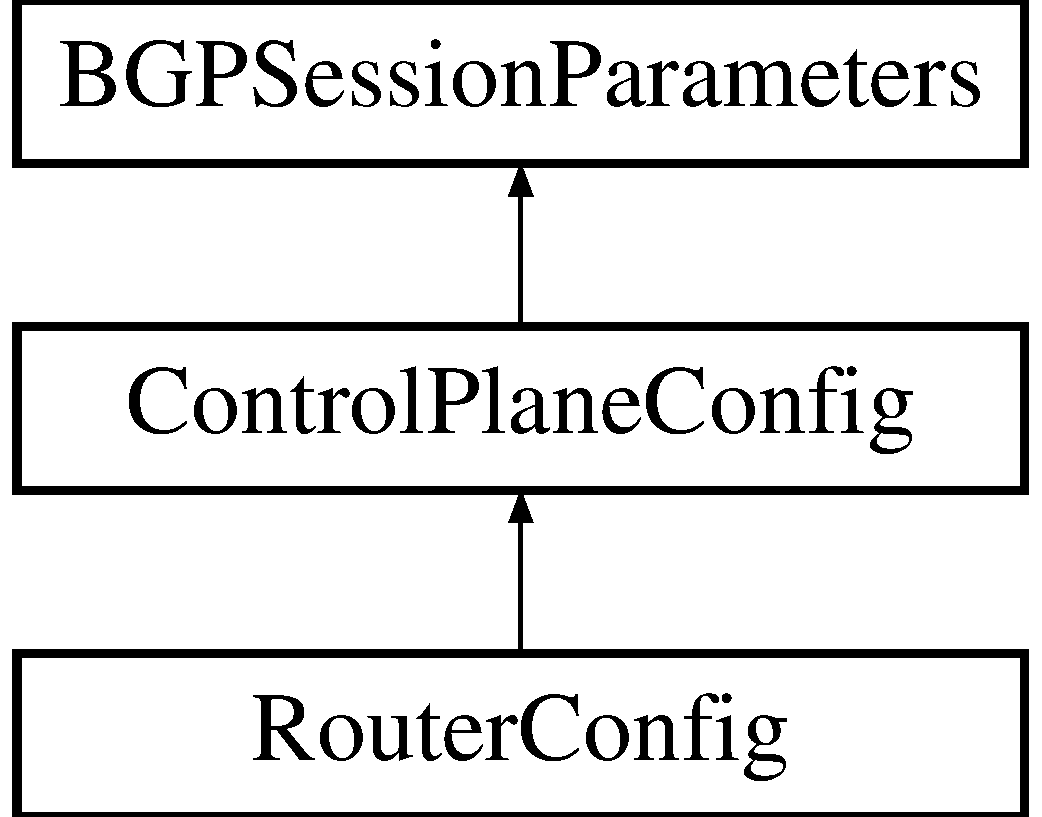
\includegraphics[height=3.000000cm]{classRouterConfig}
\end{center}
\end{figure}
\subsection*{Public Member Functions}
\begin{DoxyCompactItemize}
\item 
\hypertarget{classRouterConfig_a245e33f079a54805e0beb3497916ca5c}{\hyperlink{classRouterConfig_a245e33f079a54805e0beb3497916ca5c}{Router\-Config} (int p\-\_\-\-Number\-Of\-Interfaces)}\label{classRouterConfig_a245e33f079a54805e0beb3497916ca5c}

\begin{DoxyCompactList}\small\item\em Constructors and Destructor. \end{DoxyCompactList}\item 
\hypertarget{classRouterConfig_ab023773bfcea4de1fe396aae125979a9}{void \hyperlink{classRouterConfig_ab023773bfcea4de1fe396aae125979a9}{add\-Connection\-Config} (int p\-\_\-\-Local\-Interface\-Id, int p\-\_\-\-Neighbor\-Interface\-Id, int p\-\_\-\-Neighbor\-Router\-Id)}\label{classRouterConfig_ab023773bfcea4de1fe396aae125979a9}

\begin{DoxyCompactList}\small\item\em Setters. \end{DoxyCompactList}\item 
\hypertarget{classRouterConfig_a8ceb1f75bcb649d52e521e3133f0937d}{bool {\bfseries is\-Connection} (int p\-\_\-\-Interface\-Id)}\label{classRouterConfig_a8ceb1f75bcb649d52e521e3133f0937d}

\item 
\hypertarget{classRouterConfig_a047260a9321d06d46cab34c884c14ee7}{int {\bfseries get\-Neighbor\-Router\-Id} (int p\-\_\-\-Local\-Interface)}\label{classRouterConfig_a047260a9321d06d46cab34c884c14ee7}

\item 
\hypertarget{classRouterConfig_a0246df47bf6e9ff3c9c45be81c161787}{int {\bfseries get\-Neighbor\-Interface\-Id} (int p\-\_\-\-Local\-Interface)}\label{classRouterConfig_a0246df47bf6e9ff3c9c45be81c161787}

\item 
\hypertarget{classRouterConfig_a31ed6306e2aaf83fee80a046bdcfa7fb}{\hyperlink{classConnection}{Connection} $\ast$ {\bfseries get\-Connection} (int p\-\_\-\-Connection\-Id)}\label{classRouterConfig_a31ed6306e2aaf83fee80a046bdcfa7fb}

\item 
\hypertarget{classRouterConfig_a96ff8dc23d79b94afc220690d73eecbf}{void {\bfseries print\-N\-I\-C\-Modes} (void)}\label{classRouterConfig_a96ff8dc23d79b94afc220690d73eecbf}

\item 
\hypertarget{classRouterConfig_abfd13ba5c09c9d9544de65ae923eaaad}{string {\bfseries to\-String} (void)}\label{classRouterConfig_abfd13ba5c09c9d9544de65ae923eaaad}

\item 
\hyperlink{classRouterConfig}{Router\-Config} \& \hyperlink{classRouterConfig_ab0bb5ea6cea6663966400c69c231560b}{operator=} (const \hyperlink{classRouterConfig}{Router\-Config} \&p\-\_\-\-Original)
\begin{DoxyCompactList}\small\item\em Getters. \end{DoxyCompactList}\end{DoxyCompactItemize}
\subsection*{Data Fields}
\begin{DoxyCompactItemize}
\item 
\hypertarget{classRouterConfig_a14109cff8cff86a75f09fa502ef181f2}{\hyperlink{classConnection}{Connection} $\ast$$\ast$ \hyperlink{classRouterConfig_a14109cff8cff86a75f09fa502ef181f2}{m\-\_\-\-Neighbor\-Connections}}\label{classRouterConfig_a14109cff8cff86a75f09fa502ef181f2}

\begin{DoxyCompactList}\small\item\em Linked list that holds the connection information for each interface of the router. \end{DoxyCompactList}\end{DoxyCompactItemize}
\subsection*{Additional Inherited Members}


\subsection{Detailed Description}
Holds the parameters for a router including interface connection parameters. 

Definition at line 421 of file Configuration.\-hpp.



\subsection{Member Function Documentation}
\hypertarget{classRouterConfig_ab0bb5ea6cea6663966400c69c231560b}{\index{Router\-Config@{Router\-Config}!operator=@{operator=}}
\index{operator=@{operator=}!RouterConfig@{Router\-Config}}
\subsubsection[{operator=}]{\setlength{\rightskip}{0pt plus 5cm}{\bf Router\-Config} \& Router\-Config\-::operator= (
\begin{DoxyParamCaption}
\item[{const {\bf Router\-Config} \&}]{p\-\_\-\-Original}
\end{DoxyParamCaption}
)}}\label{classRouterConfig_ab0bb5ea6cea6663966400c69c231560b}


Getters. 

clones the passed \hyperlink{classRouterConfig}{Router\-Config} object to this object

Operators

\begin{DoxyReturn}{Returns}
reference \hyperlink{classRouterConfig}{Router\-Config}\& 
\end{DoxyReturn}


Definition at line 252 of file Configuration.\-cpp.



The documentation for this class was generated from the following files\-:\begin{DoxyCompactItemize}
\item 
/home/antipant/\-Protocol\-P\-\_\-\-Project/\hyperlink{Configuration_8hpp}{Configuration.\-hpp}\item 
/home/antipant/\-Protocol\-P\-\_\-\-Project/\hyperlink{Configuration_8cpp}{Configuration.\-cpp}\end{DoxyCompactItemize}

\hypertarget{classSimulationUI_1_1RouterModel}{\section{Simulation\-U\-I.\-Router\-Model Class Reference}
\label{classSimulationUI_1_1RouterModel}\index{Simulation\-U\-I.\-Router\-Model@{Simulation\-U\-I.\-Router\-Model}}
}
Inheritance diagram for Simulation\-U\-I.\-Router\-Model\-:\begin{figure}[H]
\begin{center}
\leavevmode
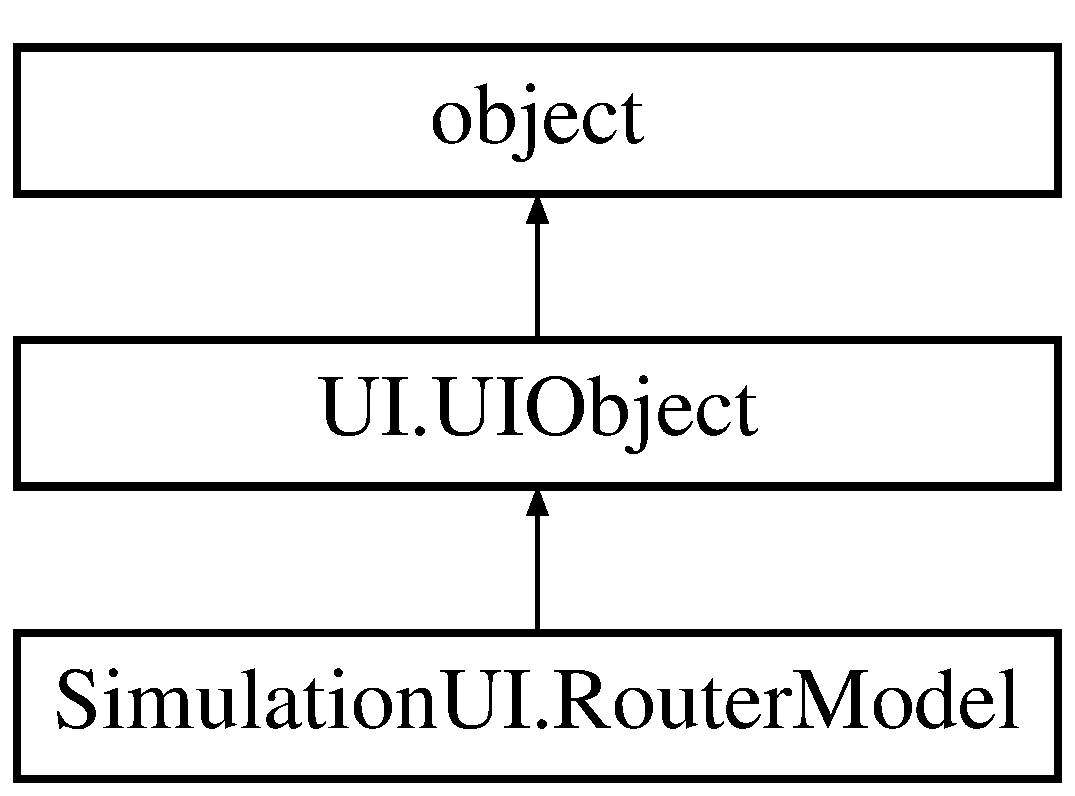
\includegraphics[height=3.000000cm]{classSimulationUI_1_1RouterModel}
\end{center}
\end{figure}
\subsection*{Public Member Functions}
\begin{DoxyCompactItemize}
\item 
\hypertarget{classSimulationUI_1_1RouterModel_a7ade1c08bc263097bafd0b045dbfdbb8}{def {\bfseries \-\_\-\-\_\-init\-\_\-\-\_\-}}\label{classSimulationUI_1_1RouterModel_a7ade1c08bc263097bafd0b045dbfdbb8}

\item 
\hypertarget{classSimulationUI_1_1RouterModel_a90ca97ae538f3baf4a3af5af42f4eb3d}{def {\bfseries draw}}\label{classSimulationUI_1_1RouterModel_a90ca97ae538f3baf4a3af5af42f4eb3d}

\item 
\hypertarget{classSimulationUI_1_1RouterModel_a79aa03f6b18ad414e182ff67d7195a24}{def {\bfseries select\-\_\-router}}\label{classSimulationUI_1_1RouterModel_a79aa03f6b18ad414e182ff67d7195a24}

\item 
\hypertarget{classSimulationUI_1_1RouterModel_a6fb15056edc3ff7c2ae96b701a1f0bd1}{def {\bfseries update\-\_\-ports}}\label{classSimulationUI_1_1RouterModel_a6fb15056edc3ff7c2ae96b701a1f0bd1}

\item 
\hypertarget{classSimulationUI_1_1RouterModel_aedb8ccdb852f603ed49c56f51e1b8793}{def {\bfseries update\-\_\-text}}\label{classSimulationUI_1_1RouterModel_aedb8ccdb852f603ed49c56f51e1b8793}

\end{DoxyCompactItemize}
\subsection*{Data Fields}
\begin{DoxyCompactItemize}
\item 
\hypertarget{classSimulationUI_1_1RouterModel_a1d3617a602c08ed680127cc257e97b87}{{\bfseries pos}}\label{classSimulationUI_1_1RouterModel_a1d3617a602c08ed680127cc257e97b87}

\item 
\hypertarget{classSimulationUI_1_1RouterModel_a8bf99e117068fbbff2d23bf9ba80a1b4}{{\bfseries parent}}\label{classSimulationUI_1_1RouterModel_a8bf99e117068fbbff2d23bf9ba80a1b4}

\item 
\hypertarget{classSimulationUI_1_1RouterModel_a6b17eb9939b93425c8f966deab59f347}{{\bfseries surface}}\label{classSimulationUI_1_1RouterModel_a6b17eb9939b93425c8f966deab59f347}

\item 
\hypertarget{classSimulationUI_1_1RouterModel_acf42147c3c9b5d79cc1b109e8d414852}{{\bfseries router}}\label{classSimulationUI_1_1RouterModel_acf42147c3c9b5d79cc1b109e8d414852}

\item 
\hypertarget{classSimulationUI_1_1RouterModel_aaa43fd3c59476472e46c55325a3feb5c}{{\bfseries selected\-\_\-port}}\label{classSimulationUI_1_1RouterModel_aaa43fd3c59476472e46c55325a3feb5c}

\item 
\hypertarget{classSimulationUI_1_1RouterModel_a9603150ce3eb99c674a396943a9ca7f0}{{\bfseries ezfont}}\label{classSimulationUI_1_1RouterModel_a9603150ce3eb99c674a396943a9ca7f0}

\item 
\hypertarget{classSimulationUI_1_1RouterModel_a39d6a3c8dd0f87d62f2850b99469929c}{{\bfseries router\-\_\-logicblock}}\label{classSimulationUI_1_1RouterModel_a39d6a3c8dd0f87d62f2850b99469929c}

\item 
\hypertarget{classSimulationUI_1_1RouterModel_a5cdecd2aad348c9aaf36e4f0ce350beb}{{\bfseries port\-\_\-blocks}}\label{classSimulationUI_1_1RouterModel_a5cdecd2aad348c9aaf36e4f0ce350beb}

\end{DoxyCompactItemize}
\subsection*{Additional Inherited Members}


\subsection{Detailed Description}


Definition at line 41 of file Simulation\-U\-I.\-py.



The documentation for this class was generated from the following file\-:\begin{DoxyCompactItemize}
\item 
/home/antipant/\-Protocol\-P\-\_\-\-Project/\-U\-I/Simulation\-U\-I.\-py\end{DoxyCompactItemize}

\hypertarget{classRoutingTable}{\section{Routing\-Table Class Reference}
\label{classRoutingTable}\index{Routing\-Table@{Routing\-Table}}
}


\hyperlink{classRoutingTable}{Routing\-Table} module.  




{\ttfamily \#include $<$Routing\-Table.\-hpp$>$}

Inheritance diagram for Routing\-Table\-:\begin{figure}[H]
\begin{center}
\leavevmode
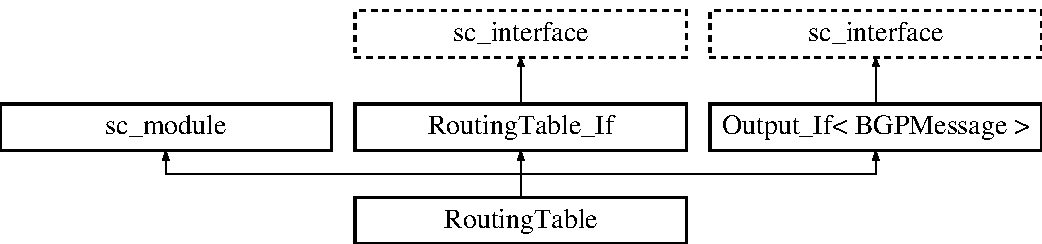
\includegraphics[height=3.000000cm]{classRoutingTable}
\end{center}
\end{figure}
\subsection*{Public Member Functions}
\begin{DoxyCompactItemize}
\item 
\hypertarget{classRoutingTable_a71a78835bd82f883251e5937cd3d9bcc}{\hyperlink{classRoutingTable_a71a78835bd82f883251e5937cd3d9bcc}{Routing\-Table} (sc\-\_\-module\-\_\-name p\-\_\-\-Module\-Name, \hyperlink{classControlPlaneConfig}{Control\-Plane\-Config} $\ast$const p\-\_\-\-R\-T\-Config)}\label{classRoutingTable_a71a78835bd82f883251e5937cd3d9bcc}

\begin{DoxyCompactList}\small\item\em Elaborates the \hyperlink{classRoutingTable}{Routing\-Table} module. \end{DoxyCompactList}\item 
\hyperlink{classRoutingTable_abe5b508511742899600b98401af7c761}{$\sim$\-Routing\-Table} ()
\begin{DoxyCompactList}\small\item\em Destructor of the \hyperlink{classRoutingTable}{Routing\-Table} module. \end{DoxyCompactList}\item 
void \hyperlink{classRoutingTable_a9cde93247eb0ec479d085c427e8c040d}{routing\-Table\-Main} (void)
\begin{DoxyCompactList}\small\item\em The main process of Control Plane module. \end{DoxyCompactList}\item 
\hypertarget{classRoutingTable_a15cac9bbc532546c14ce29d5b19772bc}{virtual int \hyperlink{classRoutingTable_a15cac9bbc532546c14ce29d5b19772bc}{resolve\-Route} (string p\-\_\-\-I\-P\-Address)}\label{classRoutingTable_a15cac9bbc532546c14ce29d5b19772bc}

\begin{DoxyCompactList}\small\item\em Set new route to the Routing \hyperlink{classTable}{Table}. \end{DoxyCompactList}\item 
\hyperlink{classRoutingTable_a6672fa1eeba99406384473815b27b6ea}{S\-C\-\_\-\-H\-A\-S\-\_\-\-P\-R\-O\-C\-E\-S\-S} (\hyperlink{classRoutingTable}{Routing\-Table})
\begin{DoxyCompactList}\small\item\em Indicate the system\-C producer that this module has a process. \end{DoxyCompactList}\item 
\hypertarget{classRoutingTable_a2d64d4f1e7d3a8cbb209633c1f50cae2}{bool {\bfseries add\-Route\-To\-Raw\-Table} (string p\-\_\-msg, int p\-\_\-output\-Port)}\label{classRoutingTable_a2d64d4f1e7d3a8cbb209633c1f50cae2}

\item 
\hypertarget{classRoutingTable_acb0fef81a119d5aa54367bbb817390bb}{void {\bfseries set\-Local\-Preference} (int p\-\_\-\-A\-S, int p\-\_\-preference\-Value)}\label{classRoutingTable_acb0fef81a119d5aa54367bbb817390bb}

\item 
\hypertarget{classRoutingTable_abb0e727faa93499d36b3f234664df133}{void {\bfseries remove\-Local\-Pref} (int p\-\_\-\-A\-S)}\label{classRoutingTable_abb0e727faa93499d36b3f234664df133}

\item 
\hypertarget{classRoutingTable_a5e3c7b755bbc5788388a47d5b3d53e1e}{void {\bfseries delete\-Route} (int p\-\_\-router1, int p\-\_\-router2)}\label{classRoutingTable_a5e3c7b755bbc5788388a47d5b3d53e1e}

\item 
\hypertarget{classRoutingTable_a63a0efbe82ccd53c0e6baa0259c7b10d}{string {\bfseries get\-Routing\-Table} ()}\label{classRoutingTable_a63a0efbe82ccd53c0e6baa0259c7b10d}

\item 
\hypertarget{classRoutingTable_aadac68ca579fe85ce4328d42acbd3e0d}{string {\bfseries get\-Raw\-Routing\-Table} ()}\label{classRoutingTable_aadac68ca579fe85ce4328d42acbd3e0d}

\item 
\hypertarget{classRoutingTable_af938852f430a4483c28e7956136fa2ab}{void {\bfseries clear\-Routing\-Tables} ()}\label{classRoutingTable_af938852f430a4483c28e7956136fa2ab}

\item 
virtual bool \hyperlink{classRoutingTable_ac54104a090c70c3f23799af1f30113e7}{write} (\hyperlink{classBGPMessage}{B\-G\-P\-Message} \&p\-\_\-\-B\-G\-P\-Msg)
\begin{DoxyCompactList}\small\item\em Allows the session to pass B\-G\-P messages to the \hyperlink{classDataPlane}{Data\-Plane}. \end{DoxyCompactList}\item 
\hypertarget{classRoutingTable_a2d688b3f2ced6fa02995086cd7a72872}{void {\bfseries kill\-Routing\-Table} (void)}\label{classRoutingTable_a2d688b3f2ced6fa02995086cd7a72872}

\item 
\hypertarget{classRoutingTable_ad765fbb07c6fdec4e1028a6a75b0762d}{void {\bfseries revive\-Routing\-Table} (void)}\label{classRoutingTable_ad765fbb07c6fdec4e1028a6a75b0762d}

\item 
\hypertarget{classRoutingTable_a9a796af2479afeecf336670f9aaaebd8}{void {\bfseries set\-Up} (bool p\-\_\-\-Value)}\label{classRoutingTable_a9a796af2479afeecf336670f9aaaebd8}

\item 
\hypertarget{classRoutingTable_a528839c68336d265c100de1fab267f8f}{bool {\bfseries is\-Running} (void)}\label{classRoutingTable_a528839c68336d265c100de1fab267f8f}

\end{DoxyCompactItemize}
\subsection*{Data Fields}
\begin{DoxyCompactItemize}
\item 
sc\-\_\-in\-\_\-clk \hyperlink{classRoutingTable_a3f57617a0dbdfabc34534eda6731da74}{port\-\_\-\-Clk}
\begin{DoxyCompactList}\small\item\em System clock signal. \end{DoxyCompactList}\item 
sc\-\_\-port$<$ \hyperlink{classBGPSession__If}{B\-G\-P\-Session\-\_\-\-If}, \\*
0, S\-C\-\_\-\-Z\-E\-R\-O\-\_\-\-O\-R\-\_\-\-M\-O\-R\-E\-\_\-\-B\-O\-U\-N\-D $>$ \hyperlink{classRoutingTable_af24047fc955ca1e81caee0468f70f62c}{port\-\_\-\-Session}
\begin{DoxyCompactList}\small\item\em Control port. \end{DoxyCompactList}\item 
sc\-\_\-port$<$ \hyperlink{classOutput__If}{Output\-\_\-\-If} $>$ \hyperlink{classRoutingTable_ac463a755c9a322a1641ae0422ee845e3}{port\-\_\-\-Output}
\begin{DoxyCompactList}\small\item\em Output port for B\-G\-P messages. \end{DoxyCompactList}\item 
bool \hyperlink{classRoutingTable_a4a4945747e35355545c416e5965b83bc}{m\-\_\-\-New\-Input\-Msg}
\begin{DoxyCompactList}\small\item\em Set new route to the Routing \hyperlink{classTable}{Table}. \end{DoxyCompactList}\end{DoxyCompactItemize}


\subsection{Detailed Description}
\hyperlink{classRoutingTable}{Routing\-Table} module. 

Routing \hyperlink{classTable}{Table} contains B\-G\-P routes and offers methods to manage, and access them 

Definition at line 45 of file Routing\-Table.\-hpp.



\subsection{Constructor \& Destructor Documentation}
\hypertarget{classRoutingTable_abe5b508511742899600b98401af7c761}{\index{Routing\-Table@{Routing\-Table}!$\sim$\-Routing\-Table@{$\sim$\-Routing\-Table}}
\index{$\sim$\-Routing\-Table@{$\sim$\-Routing\-Table}!RoutingTable@{Routing\-Table}}
\subsubsection[{$\sim$\-Routing\-Table}]{\setlength{\rightskip}{0pt plus 5cm}Routing\-Table\-::$\sim$\-Routing\-Table (
\begin{DoxyParamCaption}
{}
\end{DoxyParamCaption}
)}}\label{classRoutingTable_abe5b508511742899600b98401af7c761}


Destructor of the \hyperlink{classRoutingTable}{Routing\-Table} module. 

Free's all the dynamically allocated memory 

Definition at line 38 of file Routing\-Table.\-cpp.



\subsection{Member Function Documentation}
\hypertarget{classRoutingTable_a9cde93247eb0ec479d085c427e8c040d}{\index{Routing\-Table@{Routing\-Table}!routing\-Table\-Main@{routing\-Table\-Main}}
\index{routing\-Table\-Main@{routing\-Table\-Main}!RoutingTable@{Routing\-Table}}
\subsubsection[{routing\-Table\-Main}]{\setlength{\rightskip}{0pt plus 5cm}void Routing\-Table\-::routing\-Table\-Main (
\begin{DoxyParamCaption}
\item[{void}]{}
\end{DoxyParamCaption}
)}}\label{classRoutingTable_a9cde93247eb0ec479d085c427e8c040d}


The main process of Control Plane module. 

\begin{DoxyItemize}
\item Reads B\-G\-P messages from the m\-\_\-\-Receiving\-Buffer.\item performs the route resolution process accoriding to B\-G\-P protocol. \item Generates the required update messages.\item Keeps track on different B\-G\-P sessions. \end{DoxyItemize}
B\-G\-P notification and update output port 

Definition at line 44 of file Routing\-Table.\-cpp.

\hypertarget{classRoutingTable_a6672fa1eeba99406384473815b27b6ea}{\index{Routing\-Table@{Routing\-Table}!S\-C\-\_\-\-H\-A\-S\-\_\-\-P\-R\-O\-C\-E\-S\-S@{S\-C\-\_\-\-H\-A\-S\-\_\-\-P\-R\-O\-C\-E\-S\-S}}
\index{S\-C\-\_\-\-H\-A\-S\-\_\-\-P\-R\-O\-C\-E\-S\-S@{S\-C\-\_\-\-H\-A\-S\-\_\-\-P\-R\-O\-C\-E\-S\-S}!RoutingTable@{Routing\-Table}}
\subsubsection[{S\-C\-\_\-\-H\-A\-S\-\_\-\-P\-R\-O\-C\-E\-S\-S}]{\setlength{\rightskip}{0pt plus 5cm}Routing\-Table\-::\-S\-C\-\_\-\-H\-A\-S\-\_\-\-P\-R\-O\-C\-E\-S\-S (
\begin{DoxyParamCaption}
\item[{{\bf Routing\-Table}}]{}
\end{DoxyParamCaption}
)}}\label{classRoutingTable_a6672fa1eeba99406384473815b27b6ea}


Indicate the system\-C producer that this module has a process. 

\begin{DoxySeeAlso}{See Also}
\href{http://www.iro.umontreal.ca/~lablasso/docs/SystemC2.0.1/html/classproducer.html}{\tt http\-://www.\-iro.\-umontreal.\-ca/$\sim$lablasso/docs/\-System\-C2.\-0.\-1/html/classproducer.\-html} 
\end{DoxySeeAlso}
\hypertarget{classRoutingTable_ac54104a090c70c3f23799af1f30113e7}{\index{Routing\-Table@{Routing\-Table}!write@{write}}
\index{write@{write}!RoutingTable@{Routing\-Table}}
\subsubsection[{write}]{\setlength{\rightskip}{0pt plus 5cm}bool Routing\-Table\-::write (
\begin{DoxyParamCaption}
\item[{{\bf B\-G\-P\-Message} \&}]{}
\end{DoxyParamCaption}
)\hspace{0.3cm}{\ttfamily [virtual]}}}\label{classRoutingTable_ac54104a090c70c3f23799af1f30113e7}


Allows the session to pass B\-G\-P messages to the \hyperlink{classDataPlane}{Data\-Plane}. 

The method shall implement a mutex that takes care of the arbitraton between sessions 
\begin{DoxyParams}[1]{Parameters}
\mbox{\tt in}  & {\em \hyperlink{classBGPMessage}{B\-G\-P\-Message}} & p\-\_\-\-B\-G\-P\-Msg The B\-G\-P message to be send \\
\hline
\end{DoxyParams}
\begin{DoxyReturn}{Returns}
bool True\-: if success is valid, False\-: if not success 
\end{DoxyReturn}


Implements \hyperlink{classOutput__If_aeef0f3dff2d02e85375e914e83140602}{Output\-\_\-\-If$<$ B\-G\-P\-Message $>$}.



Definition at line 1152 of file Routing\-Table.\-cpp.



\subsection{Field Documentation}
\hypertarget{classRoutingTable_a4a4945747e35355545c416e5965b83bc}{\index{Routing\-Table@{Routing\-Table}!m\-\_\-\-New\-Input\-Msg@{m\-\_\-\-New\-Input\-Msg}}
\index{m\-\_\-\-New\-Input\-Msg@{m\-\_\-\-New\-Input\-Msg}!RoutingTable@{Routing\-Table}}
\subsubsection[{m\-\_\-\-New\-Input\-Msg}]{\setlength{\rightskip}{0pt plus 5cm}bool Routing\-Table\-::m\-\_\-\-New\-Input\-Msg}}\label{classRoutingTable_a4a4945747e35355545c416e5965b83bc}


Set new route to the Routing \hyperlink{classTable}{Table}. 

Set new route to the Routing \hyperlink{classTable}{Table} 

Definition at line 283 of file Routing\-Table.\-hpp.

\hypertarget{classRoutingTable_a3f57617a0dbdfabc34534eda6731da74}{\index{Routing\-Table@{Routing\-Table}!port\-\_\-\-Clk@{port\-\_\-\-Clk}}
\index{port\-\_\-\-Clk@{port\-\_\-\-Clk}!RoutingTable@{Routing\-Table}}
\subsubsection[{port\-\_\-\-Clk}]{\setlength{\rightskip}{0pt plus 5cm}sc\-\_\-in\-\_\-clk Routing\-Table\-::port\-\_\-\-Clk}}\label{classRoutingTable_a3f57617a0dbdfabc34534eda6731da74}


System clock signal. 

The router's internal clock 

Definition at line 55 of file Routing\-Table.\-hpp.

\hypertarget{classRoutingTable_ac463a755c9a322a1641ae0422ee845e3}{\index{Routing\-Table@{Routing\-Table}!port\-\_\-\-Output@{port\-\_\-\-Output}}
\index{port\-\_\-\-Output@{port\-\_\-\-Output}!RoutingTable@{Routing\-Table}}
\subsubsection[{port\-\_\-\-Output}]{\setlength{\rightskip}{0pt plus 5cm}sc\-\_\-port$<${\bf Output\-\_\-\-If}$>$ Routing\-Table\-::port\-\_\-\-Output}}\label{classRoutingTable_ac463a755c9a322a1641ae0422ee845e3}


Output port for B\-G\-P messages. 

The \hyperlink{classRoutingTable}{Routing\-Table} writes all the B\-G\-P messages to be send to its neighbors into this port. The port should be bind to the Data Plane's. receiving F\-I\-F\-O 

Definition at line 72 of file Routing\-Table.\-hpp.

\hypertarget{classRoutingTable_af24047fc955ca1e81caee0468f70f62c}{\index{Routing\-Table@{Routing\-Table}!port\-\_\-\-Session@{port\-\_\-\-Session}}
\index{port\-\_\-\-Session@{port\-\_\-\-Session}!RoutingTable@{Routing\-Table}}
\subsubsection[{port\-\_\-\-Session}]{\setlength{\rightskip}{0pt plus 5cm}sc\-\_\-port$<${\bf B\-G\-P\-Session\-\_\-\-If}, 0, S\-C\-\_\-\-Z\-E\-R\-O\-\_\-\-O\-R\-\_\-\-M\-O\-R\-E\-\_\-\-B\-O\-U\-N\-D$>$ Routing\-Table\-::port\-\_\-\-Session}}\label{classRoutingTable_af24047fc955ca1e81caee0468f70f62c}


Control port. 

Routing table can check through this port whether the network interfaces are up or not. 

Definition at line 63 of file Routing\-Table.\-hpp.



The documentation for this class was generated from the following files\-:\begin{DoxyCompactItemize}
\item 
/home/antipant/\-Protocol\-P\-\_\-\-Project/\hyperlink{RoutingTable_8hpp}{Routing\-Table.\-hpp}\item 
/home/antipant/\-Protocol\-P\-\_\-\-Project/\hyperlink{RoutingTable_8cpp}{Routing\-Table.\-cpp}\end{DoxyCompactItemize}

\hypertarget{classSimulationUI_1_1RoutingTable}{\section{Simulation\-U\-I.\-Routing\-Table Class Reference}
\label{classSimulationUI_1_1RoutingTable}\index{Simulation\-U\-I.\-Routing\-Table@{Simulation\-U\-I.\-Routing\-Table}}
}
\subsection*{Public Member Functions}
\begin{DoxyCompactItemize}
\item 
\hypertarget{classSimulationUI_1_1RoutingTable_ac3e4dbcd347a2fc61d4f368cefc7f909}{def {\bfseries \-\_\-\-\_\-init\-\_\-\-\_\-}}\label{classSimulationUI_1_1RoutingTable_ac3e4dbcd347a2fc61d4f368cefc7f909}

\item 
\hypertarget{classSimulationUI_1_1RoutingTable_a5d3e0cc1f5b5a48c381ee9bd0cc00752}{def {\bfseries update\-\_\-table}}\label{classSimulationUI_1_1RoutingTable_a5d3e0cc1f5b5a48c381ee9bd0cc00752}

\end{DoxyCompactItemize}
\subsection*{Data Fields}
\begin{DoxyCompactItemize}
\item 
\hypertarget{classSimulationUI_1_1RoutingTable_a7fa4c188db44860d9facf2cf5ff9dbc8}{{\bfseries table}}\label{classSimulationUI_1_1RoutingTable_a7fa4c188db44860d9facf2cf5ff9dbc8}

\end{DoxyCompactItemize}


\subsection{Detailed Description}


Definition at line 215 of file Simulation\-U\-I.\-py.



The documentation for this class was generated from the following file\-:\begin{DoxyCompactItemize}
\item 
/home/antipant/\-Protocol\-P\-\_\-\-Project/\-U\-I/Simulation\-U\-I.\-py\end{DoxyCompactItemize}

\hypertarget{classRoutingTable__If}{\section{Routing\-Table\-\_\-\-If Class Reference}
\label{classRoutingTable__If}\index{Routing\-Table\-\_\-\-If@{Routing\-Table\-\_\-\-If}}
}
Inheritance diagram for Routing\-Table\-\_\-\-If\-:\begin{figure}[H]
\begin{center}
\leavevmode
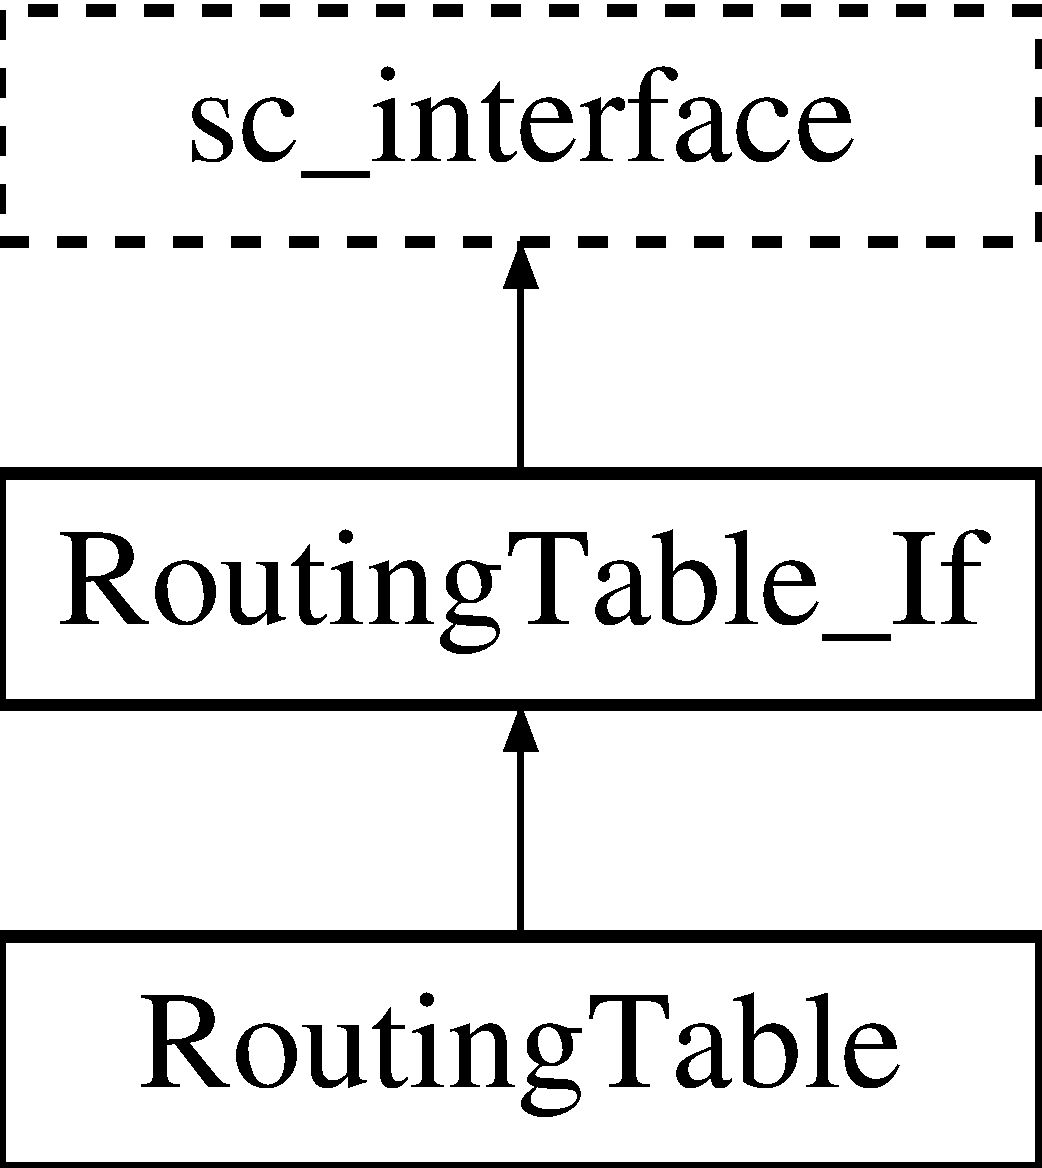
\includegraphics[height=3.000000cm]{classRoutingTable__If}
\end{center}
\end{figure}
\subsection*{Public Member Functions}
\begin{DoxyCompactItemize}
\item 
\hypertarget{classRoutingTable__If_af6210909231b656e415fa3c748db6e4f}{virtual int \hyperlink{classRoutingTable__If_af6210909231b656e415fa3c748db6e4f}{resolve\-Route} (string p\-\_\-\-I\-P\-Address)=0}\label{classRoutingTable__If_af6210909231b656e415fa3c748db6e4f}

\begin{DoxyCompactList}\small\item\em Set new route to the Routing \hyperlink{classTable}{Table}. \end{DoxyCompactList}\end{DoxyCompactItemize}


\subsection{Detailed Description}


Definition at line 28 of file Routing\-Table\-\_\-\-If.\-hpp.



The documentation for this class was generated from the following file\-:\begin{DoxyCompactItemize}
\item 
/home/antipant/\-Protocol\-P\-\_\-\-Project/\hyperlink{RoutingTable__If_8hpp}{Routing\-Table\-\_\-\-If.\-hpp}\end{DoxyCompactItemize}

\hypertarget{classselectdialog_1_1ScrollBar}{\section{selectdialog.\-Scroll\-Bar Class Reference}
\label{classselectdialog_1_1ScrollBar}\index{selectdialog.\-Scroll\-Bar@{selectdialog.\-Scroll\-Bar}}
}
Inheritance diagram for selectdialog.\-Scroll\-Bar\-:\begin{figure}[H]
\begin{center}
\leavevmode
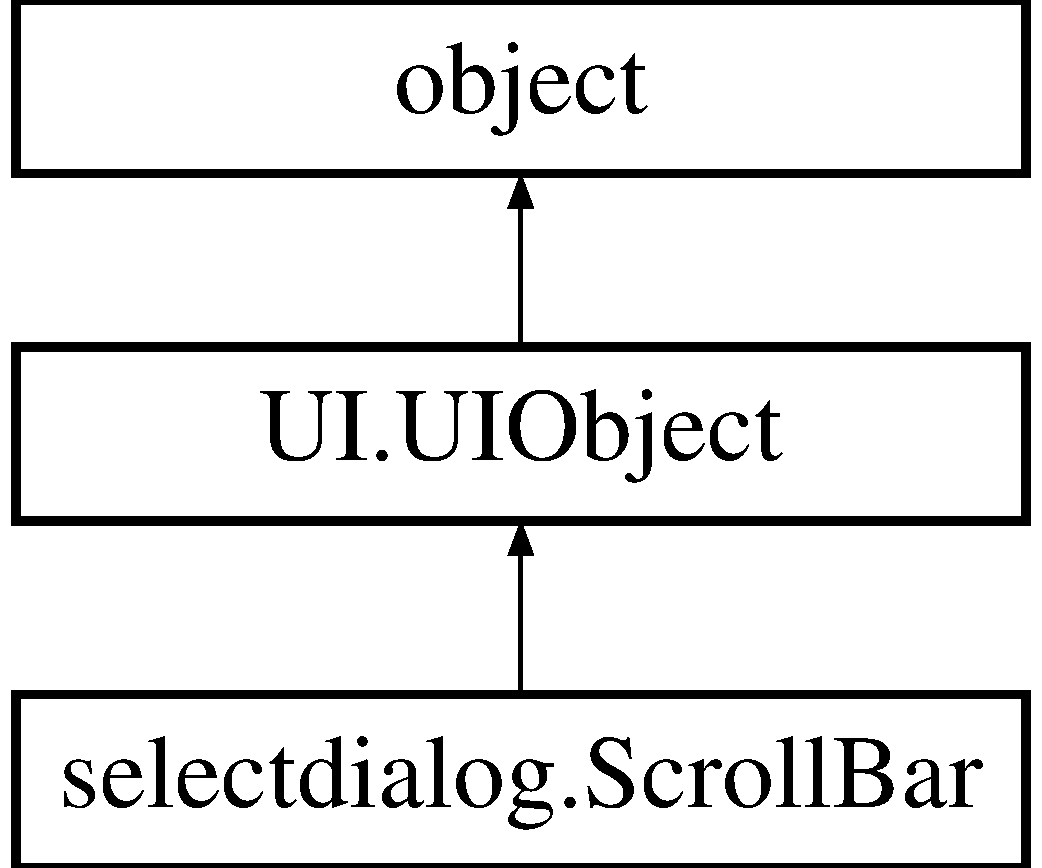
\includegraphics[height=3.000000cm]{classselectdialog_1_1ScrollBar}
\end{center}
\end{figure}
\subsection*{Public Member Functions}
\begin{DoxyCompactItemize}
\item 
\hypertarget{classselectdialog_1_1ScrollBar_a3375710b6598051346ce2975d02c9241}{def {\bfseries \-\_\-\-\_\-init\-\_\-\-\_\-}}\label{classselectdialog_1_1ScrollBar_a3375710b6598051346ce2975d02c9241}

\item 
\hypertarget{classselectdialog_1_1ScrollBar_a7bf13e4b604a0f0310d3277100181190}{def {\bfseries event}}\label{classselectdialog_1_1ScrollBar_a7bf13e4b604a0f0310d3277100181190}

\end{DoxyCompactItemize}
\subsection*{Data Fields}
\begin{DoxyCompactItemize}
\item 
\hypertarget{classselectdialog_1_1ScrollBar_ace5ef6ca6a29a08e3db0a8a081608ed6}{{\bfseries knob}}\label{classselectdialog_1_1ScrollBar_ace5ef6ca6a29a08e3db0a8a081608ed6}

\item 
\hypertarget{classselectdialog_1_1ScrollBar_a3e65a342db23bc06d679ca3bdca229a8}{{\bfseries leeway}}\label{classselectdialog_1_1ScrollBar_a3e65a342db23bc06d679ca3bdca229a8}

\item 
\hypertarget{classselectdialog_1_1ScrollBar_aa1cfe0c9dea47744a2561fbe6dba74fa}{{\bfseries range}}\label{classselectdialog_1_1ScrollBar_aa1cfe0c9dea47744a2561fbe6dba74fa}

\end{DoxyCompactItemize}
\subsection*{Properties}
\begin{DoxyCompactItemize}
\item 
\hypertarget{classselectdialog_1_1ScrollBar_a31ff84ff656c43eec236f25b2586d8a5}{{\bfseries value} = property(\-\_\-get\-\_\-value, \-\_\-set\-\_\-value)}\label{classselectdialog_1_1ScrollBar_a31ff84ff656c43eec236f25b2586d8a5}

\end{DoxyCompactItemize}


\subsection{Detailed Description}


Definition at line 113 of file selectdialog.\-py.



The documentation for this class was generated from the following file\-:\begin{DoxyCompactItemize}
\item 
/home/antipant/\-Protocol\-P\-\_\-\-Project/\-U\-I/selectdialog.\-py\end{DoxyCompactItemize}

\hypertarget{classServerSocket}{\section{Server\-Socket Class Reference}
\label{classServerSocket}\index{Server\-Socket@{Server\-Socket}}
}


Definition of the \hyperlink{classServerSocket}{Server\-Socket} class.  




{\ttfamily \#include $<$Server\-Socket.\-h$>$}

Inheritance diagram for Server\-Socket\-:\begin{figure}[H]
\begin{center}
\leavevmode
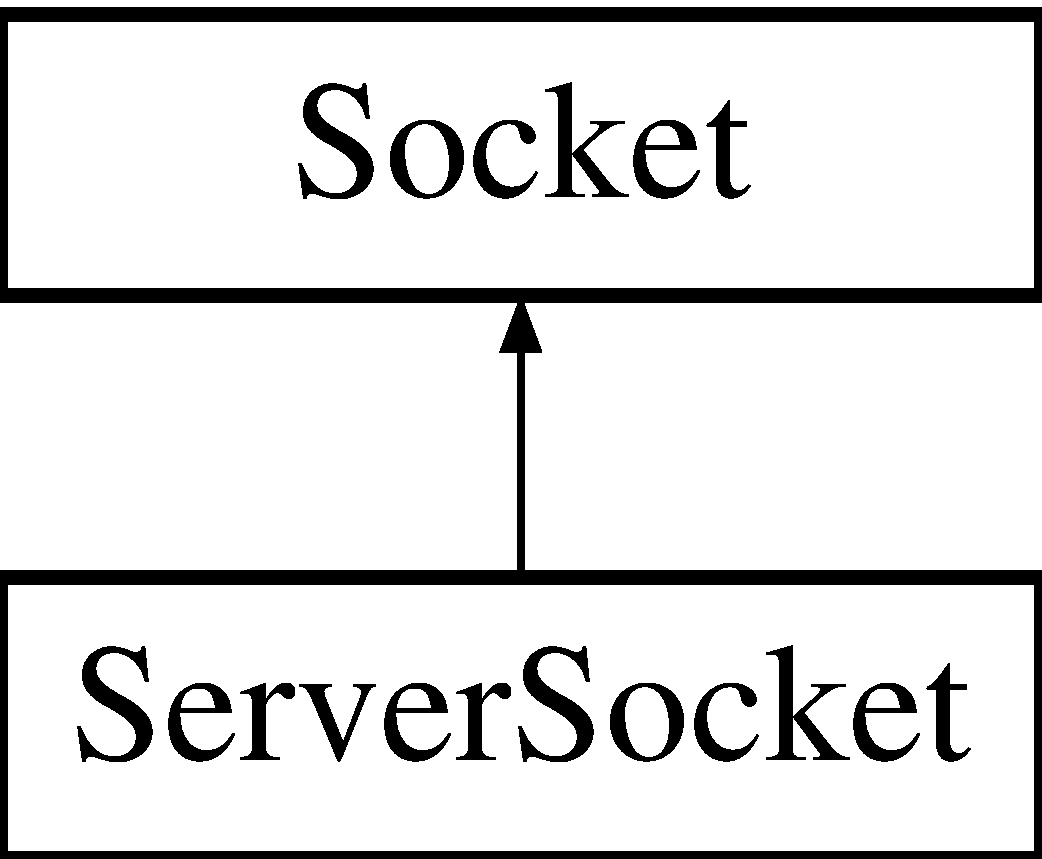
\includegraphics[height=2.000000cm]{classServerSocket}
\end{center}
\end{figure}
\subsection*{Public Member Functions}
\begin{DoxyCompactItemize}
\item 
\hypertarget{classServerSocket_a3dc1a31f740e4a8d69ae10c5dcb547d6}{{\bfseries Server\-Socket} (int port)}\label{classServerSocket_a3dc1a31f740e4a8d69ae10c5dcb547d6}

\item 
\hypertarget{classServerSocket_ab5fe4b2d92d7014f7663c1bbacbbeda5}{const \hyperlink{classServerSocket}{Server\-Socket} \& {\bfseries operator$<$$<$} (const std\-::string \&) const }\label{classServerSocket_ab5fe4b2d92d7014f7663c1bbacbbeda5}

\item 
\hypertarget{classServerSocket_a6bfabf01766bdb2c7f53274d8d771212}{const \hyperlink{classServerSocket}{Server\-Socket} \& {\bfseries operator$>$$>$} (std\-::string \&) const }\label{classServerSocket_a6bfabf01766bdb2c7f53274d8d771212}

\item 
\hypertarget{classServerSocket_ae550e314a988575d05b1dec1c3c18020}{void {\bfseries accept} (\hyperlink{classServerSocket}{Server\-Socket} \&)}\label{classServerSocket_ae550e314a988575d05b1dec1c3c18020}

\end{DoxyCompactItemize}


\subsection{Detailed Description}
Definition of the \hyperlink{classServerSocket}{Server\-Socket} class. 

Definition at line 24 of file Server\-Socket.\-h.



The documentation for this class was generated from the following files\-:\begin{DoxyCompactItemize}
\item 
/home/antipant/\-Protocol\-P\-\_\-\-Project/\hyperlink{ServerSocket_8h}{Server\-Socket.\-h}\item 
/home/antipant/\-Protocol\-P\-\_\-\-Project/\hyperlink{ServerSocket_8cpp}{Server\-Socket.\-cpp}\end{DoxyCompactItemize}

\hypertarget{classSimulation}{\section{Simulation Class Reference}
\label{classSimulation}\index{Simulation@{Simulation}}
}


\hyperlink{classSimulation}{Simulation} top module.  




{\ttfamily \#include $<$Simulation.\-hpp$>$}

Inheritance diagram for Simulation\-:\begin{figure}[H]
\begin{center}
\leavevmode
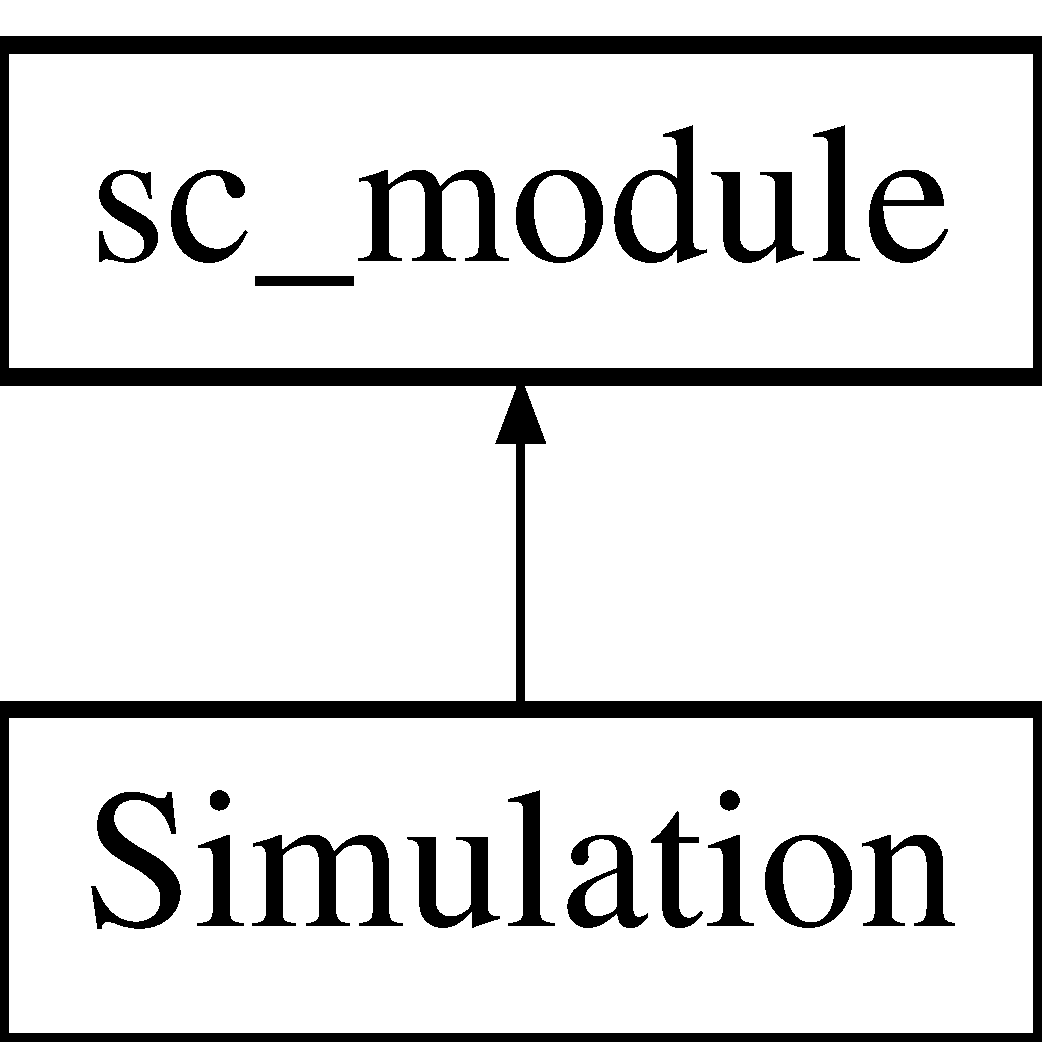
\includegraphics[height=2.000000cm]{classSimulation}
\end{center}
\end{figure}
\subsection*{Public Member Functions}
\begin{DoxyCompactItemize}
\item 
\hyperlink{classSimulation_aa163d3b4d5be9400573bb651087130d3}{Simulation} (sc\-\_\-module\-\_\-name p\-\_\-\-Name, \hyperlink{classServerSocket}{Server\-Socket} \&p\-\_\-\-Socket, \hyperlink{classSimulationConfig}{Simulation\-Config} $\ast$const p\-\_\-\-Simu\-Configuration)
\begin{DoxyCompactList}\small\item\em Constructor. \end{DoxyCompactList}\item 
\hyperlink{classSimulation_a80fad3f57dfaf195a36f7bc49bc88279}{$\sim$\-Simulation} ()
\item 
void \hyperlink{classSimulation_a313c740e616b0165c7d36f6835e61c5a}{simulation\-Main} (void)
\item 
\hypertarget{classSimulation_ab947ad2db5f5fb5a875349b2957480bd}{{\bfseries S\-C\-\_\-\-H\-A\-S\-\_\-\-P\-R\-O\-C\-E\-S\-S} (\hyperlink{classSimulation}{Simulation})}\label{classSimulation_ab947ad2db5f5fb5a875349b2957480bd}

\end{DoxyCompactItemize}
\subsection*{Data Fields}
\begin{DoxyCompactItemize}
\item 
\hypertarget{classSimulation_aeab788f0684ab0b28b3843c2b3b439a1}{sc\-\_\-in\-\_\-clk {\bfseries port\-\_\-\-Clk}}\label{classSimulation_aeab788f0684ab0b28b3843c2b3b439a1}

\end{DoxyCompactItemize}


\subsection{Detailed Description}
\hyperlink{classSimulation}{Simulation} top module. 

Definition at line 116 of file Simulation.\-hpp.



\subsection{Constructor \& Destructor Documentation}
\hypertarget{classSimulation_aa163d3b4d5be9400573bb651087130d3}{\index{Simulation@{Simulation}!Simulation@{Simulation}}
\index{Simulation@{Simulation}!Simulation@{Simulation}}
\subsubsection[{Simulation}]{\setlength{\rightskip}{0pt plus 5cm}Simulation\-::\-Simulation (
\begin{DoxyParamCaption}
\item[{sc\-\_\-module\-\_\-name}]{p\-\_\-\-Name, }
\item[{{\bf Server\-Socket} \&}]{p\-\_\-\-Socket, }
\item[{{\bf Simulation\-Config} $\ast$const}]{p\-\_\-\-Simu\-Configuration}
\end{DoxyParamCaption}
)}}\label{classSimulation_aa163d3b4d5be9400573bb651087130d3}


Constructor. 

Builds the simulation 
\begin{DoxyParams}[1]{Parameters}
\mbox{\tt in}  & {\em p\-\_\-\-Name} & The name of the module \\
\hline
\end{DoxyParams}
\begin{DoxyItemize}
\item Allocate \hyperlink{classRouter}{Router} pointer array\end{DoxyItemize}
\begin{DoxyItemize}
\item Set the base name for the \hyperlink{classStringTools}{String\-Tools} object\end{DoxyItemize}
\begin{DoxyItemize}
\item Initiate the \hyperlink{classRouter}{Router} modules as m\-\_\-\-Router\end{DoxyItemize}
\begin{DoxyItemize}
\item Generate the routers\end{DoxyItemize}
Build the network

connect all the routers

get handle to the routers configuration object

connect all the interfaces

Connect only those interfaces that have been configured

Connect the interfaces 

Definition at line 14 of file Simulation.\-cpp.

\hypertarget{classSimulation_a80fad3f57dfaf195a36f7bc49bc88279}{\index{Simulation@{Simulation}!$\sim$\-Simulation@{$\sim$\-Simulation}}
\index{$\sim$\-Simulation@{$\sim$\-Simulation}!Simulation@{Simulation}}
\subsubsection[{$\sim$\-Simulation}]{\setlength{\rightskip}{0pt plus 5cm}Simulation\-::$\sim$\-Simulation (
\begin{DoxyParamCaption}
{}
\end{DoxyParamCaption}
)}}\label{classSimulation_a80fad3f57dfaf195a36f7bc49bc88279}
\begin{DoxyItemize}
\item Free all the memory \end{DoxyItemize}


Definition at line 84 of file Simulation.\-cpp.



\subsection{Member Function Documentation}
\hypertarget{classSimulation_a313c740e616b0165c7d36f6835e61c5a}{\index{Simulation@{Simulation}!simulation\-Main@{simulation\-Main}}
\index{simulation\-Main@{simulation\-Main}!Simulation@{Simulation}}
\subsubsection[{simulation\-Main}]{\setlength{\rightskip}{0pt plus 5cm}void Simulation\-::simulation\-Main (
\begin{DoxyParamCaption}
\item[{void}]{}
\end{DoxyParamCaption}
)}}\label{classSimulation_a313c740e616b0165c7d36f6835e61c5a}
S\-T\-A\-R\-T\-:F\-S\-M of the socket server

E\-N\-D\-:F\-S\-M of the socket server 

Definition at line 95 of file Simulation.\-cpp.



The documentation for this class was generated from the following files\-:\begin{DoxyCompactItemize}
\item 
/home/antipant/\-Protocol\-P\-\_\-\-Project/\hyperlink{Simulation_8hpp}{Simulation.\-hpp}\item 
/home/antipant/\-Protocol\-P\-\_\-\-Project/\hyperlink{Simulation_8cpp}{Simulation.\-cpp}\end{DoxyCompactItemize}

\hypertarget{classSimulationConfig}{\section{Simulation\-Config Class Reference}
\label{classSimulationConfig}\index{Simulation\-Config@{Simulation\-Config}}
}


Holds all the simulation parameters received from G\-U\-I.  




{\ttfamily \#include $<$Configuration.\-hpp$>$}

\subsection*{Public Member Functions}
\begin{DoxyCompactItemize}
\item 
\hypertarget{classSimulationConfig_ab3138278034afec998556d14f962279d}{{\bfseries Simulation\-Config} (int p\-\_\-\-Number\-Of\-Routers)}\label{classSimulationConfig_ab3138278034afec998556d14f962279d}

\item 
\hypertarget{classSimulationConfig_a33a33ed001652269877187a5dba500e8}{void {\bfseries init} (int p\-\_\-\-Number\-Of\-Routers)}\label{classSimulationConfig_a33a33ed001652269877187a5dba500e8}

\item 
\hypertarget{classSimulationConfig_a4d3f7e7012dae6304dd35e1c2f8fba60}{void {\bfseries add\-Router\-Config} (int p\-\_\-\-Router\-Id, int p\-\_\-\-Number\-Of\-Interfaces)}\label{classSimulationConfig_a4d3f7e7012dae6304dd35e1c2f8fba60}

\item 
\hypertarget{classSimulationConfig_a05a2f2aa506808c1d65c21beeb91d875}{void {\bfseries add\-Connection\-Config} (int p\-\_\-\-Local\-Router\-Id, int p\-\_\-\-Local\-Interface\-Id, int p\-\_\-\-Neighbor\-Interface\-Id, int p\-\_\-\-Neighbor\-Router\-Id)}\label{classSimulationConfig_a05a2f2aa506808c1d65c21beeb91d875}

\item 
\hypertarget{classSimulationConfig_ad270719409152a88ce192dbb7f3cbff2}{void {\bfseries add\-B\-G\-P\-Session\-Parameters} (int p\-\_\-\-Local\-Router\-Id, int p\-\_\-\-Keepalive\-Time, int p\-\_\-\-Hold\-Down\-Time\-Factor)}\label{classSimulationConfig_ad270719409152a88ce192dbb7f3cbff2}

\item 
void \hyperlink{classSimulationConfig_aa7665120bc7e38768ec483e5c1daada7}{set\-Number\-Of\-Routers} (int p\-\_\-\-Number\-Of\-Routers)
\begin{DoxyCompactList}\small\item\em Sets the number of routers used in this simulation. \end{DoxyCompactList}\item 
int \hyperlink{classSimulationConfig_a5523c4c41cdd0b094dc3d84e0c310058}{get\-Number\-Of\-Routers} (void)
\begin{DoxyCompactList}\small\item\em Returns the number of routers in the simulation. \end{DoxyCompactList}\item 
\hyperlink{classRouterConfig}{Router\-Config} \& \hyperlink{classSimulationConfig_a66aa890c0bdae066484b14adc6e056e7}{get\-Router\-Configuration} (int p\-\_\-\-Router\-Id)
\begin{DoxyCompactList}\small\item\em Returns the reference to the Router\-Config-\/object defined by p\-\_\-\-Router\-Id. \end{DoxyCompactList}\item 
\hypertarget{classSimulationConfig_a753beeec5358a2fb222588801d31b24e}{\hyperlink{classRouterConfig}{Router\-Config} $\ast$ {\bfseries get\-Router\-Configuration\-Ptr} (int p\-\_\-\-Router\-Id)}\label{classSimulationConfig_a753beeec5358a2fb222588801d31b24e}

\item 
\hypertarget{classSimulationConfig_a6e8ea0a98f3e04be129501eb2a024310}{\hyperlink{classConnection}{Connection} $\ast$ {\bfseries get\-Host\-Configuration\-Ptr} (int p\-\_\-\-Router\-Id)}\label{classSimulationConfig_a6e8ea0a98f3e04be129501eb2a024310}

\item 
\hypertarget{classSimulationConfig_a824111112a0ddc0cd9bfc532cce663fc}{\hyperlink{classSimulationConfig}{Simulation\-Config} \& \hyperlink{classSimulationConfig_a824111112a0ddc0cd9bfc532cce663fc}{operator=} (const \hyperlink{classSimulationConfig}{Simulation\-Config} \&p\-\_\-\-Original)}\label{classSimulationConfig_a824111112a0ddc0cd9bfc532cce663fc}

\begin{DoxyCompactList}\small\item\em Operators. \end{DoxyCompactList}\item 
\hypertarget{classSimulationConfig_adbc183975c7dfca169c53647e276998c}{void {\bfseries if\-Modes} (void)}\label{classSimulationConfig_adbc183975c7dfca169c53647e276998c}

\item 
\hypertarget{classSimulationConfig_aa4c6f7793fc34671aa0a1a277d187525}{string {\bfseries to\-String} (void)}\label{classSimulationConfig_aa4c6f7793fc34671aa0a1a277d187525}

\end{DoxyCompactItemize}
\subsection*{Data Fields}
\begin{DoxyCompactItemize}
\item 
\hypertarget{classSimulationConfig_ae984d530f8e326656bb1736880c0156f}{int \hyperlink{classSimulationConfig_ae984d530f8e326656bb1736880c0156f}{m\-\_\-\-Number\-Of\-Routers}}\label{classSimulationConfig_ae984d530f8e326656bb1736880c0156f}

\begin{DoxyCompactList}\small\item\em Number of routers that this simulation should allocate. \end{DoxyCompactList}\end{DoxyCompactItemize}


\subsection{Detailed Description}
Holds all the simulation parameters received from G\-U\-I. 

\hyperlink{classSimulationConfig}{Simulation\-Config}

Used to build up the simulatin environment 

Definition at line 471 of file Configuration.\-hpp.



\subsection{Member Function Documentation}
\hypertarget{classSimulationConfig_a5523c4c41cdd0b094dc3d84e0c310058}{\index{Simulation\-Config@{Simulation\-Config}!get\-Number\-Of\-Routers@{get\-Number\-Of\-Routers}}
\index{get\-Number\-Of\-Routers@{get\-Number\-Of\-Routers}!SimulationConfig@{Simulation\-Config}}
\subsubsection[{get\-Number\-Of\-Routers}]{\setlength{\rightskip}{0pt plus 5cm}int Simulation\-Config\-::get\-Number\-Of\-Routers (
\begin{DoxyParamCaption}
\item[{void}]{}
\end{DoxyParamCaption}
)}}\label{classSimulationConfig_a5523c4c41cdd0b094dc3d84e0c310058}


Returns the number of routers in the simulation. 

\begin{DoxyReturn}{Returns}
integer value 
\end{DoxyReturn}


Definition at line 381 of file Configuration.\-cpp.

\hypertarget{classSimulationConfig_a66aa890c0bdae066484b14adc6e056e7}{\index{Simulation\-Config@{Simulation\-Config}!get\-Router\-Configuration@{get\-Router\-Configuration}}
\index{get\-Router\-Configuration@{get\-Router\-Configuration}!SimulationConfig@{Simulation\-Config}}
\subsubsection[{get\-Router\-Configuration}]{\setlength{\rightskip}{0pt plus 5cm}{\bf Router\-Config} \& Simulation\-Config\-::get\-Router\-Configuration (
\begin{DoxyParamCaption}
\item[{int}]{p\-\_\-\-Router\-Id}
\end{DoxyParamCaption}
)}}\label{classSimulationConfig_a66aa890c0bdae066484b14adc6e056e7}


Returns the reference to the Router\-Config-\/object defined by p\-\_\-\-Router\-Id. 

\begin{DoxyReturn}{Returns}
reference to \hyperlink{classRouterConfig}{Router\-Config} object 
\end{DoxyReturn}


Definition at line 383 of file Configuration.\-cpp.

\hypertarget{classSimulationConfig_aa7665120bc7e38768ec483e5c1daada7}{\index{Simulation\-Config@{Simulation\-Config}!set\-Number\-Of\-Routers@{set\-Number\-Of\-Routers}}
\index{set\-Number\-Of\-Routers@{set\-Number\-Of\-Routers}!SimulationConfig@{Simulation\-Config}}
\subsubsection[{set\-Number\-Of\-Routers}]{\setlength{\rightskip}{0pt plus 5cm}void Simulation\-Config\-::set\-Number\-Of\-Routers (
\begin{DoxyParamCaption}
\item[{int}]{p\-\_\-\-Number\-Of\-Routers}
\end{DoxyParamCaption}
)}}\label{classSimulationConfig_aa7665120bc7e38768ec483e5c1daada7}


Sets the number of routers used in this simulation. 


\begin{DoxyParams}[1]{Parameters}
\mbox{\tt in}  & {\em int} & p\-\_\-\-Number\-Of\-Routers The router count \\
\hline
\end{DoxyParams}


Definition at line 376 of file Configuration.\-cpp.



The documentation for this class was generated from the following files\-:\begin{DoxyCompactItemize}
\item 
/home/antipant/\-Protocol\-P\-\_\-\-Project/\hyperlink{Configuration_8hpp}{Configuration.\-hpp}\item 
/home/antipant/\-Protocol\-P\-\_\-\-Project/\hyperlink{Configuration_8cpp}{Configuration.\-cpp}\end{DoxyCompactItemize}

\hypertarget{classSimulationUI_1_1SimulationUI}{\section{Simulation\-U\-I.\-Simulation\-U\-I Class Reference}
\label{classSimulationUI_1_1SimulationUI}\index{Simulation\-U\-I.\-Simulation\-U\-I@{Simulation\-U\-I.\-Simulation\-U\-I}}
}
\subsection*{Public Member Functions}
\begin{DoxyCompactItemize}
\item 
\hypertarget{classSimulationUI_1_1SimulationUI_a7f6966f46668ae0d80410e19d1b50671}{def {\bfseries \-\_\-\-\_\-init\-\_\-\-\_\-}}\label{classSimulationUI_1_1SimulationUI_a7f6966f46668ae0d80410e19d1b50671}

\item 
\hypertarget{classSimulationUI_1_1SimulationUI_a4c431afe0340c73372b92fdb6b5e2f7f}{def {\bfseries add\-\_\-router}}\label{classSimulationUI_1_1SimulationUI_a4c431afe0340c73372b92fdb6b5e2f7f}

\item 
\hypertarget{classSimulationUI_1_1SimulationUI_ad6cfb7a6fafaf8d97c581db74797638d}{def {\bfseries clear\-\_\-packets}}\label{classSimulationUI_1_1SimulationUI_ad6cfb7a6fafaf8d97c581db74797638d}

\item 
\hypertarget{classSimulationUI_1_1SimulationUI_a9413db668bbae20bd366dfd45fb31f2d}{def {\bfseries send\-\_\-cmd}}\label{classSimulationUI_1_1SimulationUI_a9413db668bbae20bd366dfd45fb31f2d}

\item 
\hypertarget{classSimulationUI_1_1SimulationUI_acc3bcf95c305e3599a1b31a5f0069f42}{def {\bfseries log}}\label{classSimulationUI_1_1SimulationUI_acc3bcf95c305e3599a1b31a5f0069f42}

\item 
\hypertarget{classSimulationUI_1_1SimulationUI_a12e480a3e97e54b5e1dc595e2fc62348}{def {\bfseries print\-\_\-help}}\label{classSimulationUI_1_1SimulationUI_a12e480a3e97e54b5e1dc595e2fc62348}

\item 
\hypertarget{classSimulationUI_1_1SimulationUI_a59be81b3c9e11646fdc205723e18d705}{def {\bfseries print\-\_\-conf\-\_\-help}}\label{classSimulationUI_1_1SimulationUI_a59be81b3c9e11646fdc205723e18d705}

\item 
\hypertarget{classSimulationUI_1_1SimulationUI_a82a5eb79fe6f5b227a18aead38748c5d}{def {\bfseries print\-\_\-sim\-\_\-help}}\label{classSimulationUI_1_1SimulationUI_a82a5eb79fe6f5b227a18aead38748c5d}

\item 
\hypertarget{classSimulationUI_1_1SimulationUI_a4865bdfd0ae608951805410f277ea1a1}{def {\bfseries connect}}\label{classSimulationUI_1_1SimulationUI_a4865bdfd0ae608951805410f277ea1a1}

\item 
\hypertarget{classSimulationUI_1_1SimulationUI_aaa4c6c8232b7add3580d2bcf3f5957dc}{def {\bfseries disconnect}}\label{classSimulationUI_1_1SimulationUI_aaa4c6c8232b7add3580d2bcf3f5957dc}

\item 
\hypertarget{classSimulationUI_1_1SimulationUI_a5827f55359483b0cfadbb0ca8a67b4fa}{def {\bfseries next\-\_\-free\-\_\-port}}\label{classSimulationUI_1_1SimulationUI_a5827f55359483b0cfadbb0ca8a67b4fa}

\item 
\hypertarget{classSimulationUI_1_1SimulationUI_ab4d40db66313e99a5d2c555f94579262}{def {\bfseries send\-\_\-packet}}\label{classSimulationUI_1_1SimulationUI_ab4d40db66313e99a5d2c555f94579262}

\item 
\hypertarget{classSimulationUI_1_1SimulationUI_ada015ee02a212dfb115c762fb2a6d685}{def {\bfseries add\-\_\-route}}\label{classSimulationUI_1_1SimulationUI_ada015ee02a212dfb115c762fb2a6d685}

\item 
\hypertarget{classSimulationUI_1_1SimulationUI_a83a16b2f5c49b9b32a7a9b034cdab804}{def {\bfseries remove\-\_\-route}}\label{classSimulationUI_1_1SimulationUI_a83a16b2f5c49b9b32a7a9b034cdab804}

\item 
\hypertarget{classSimulationUI_1_1SimulationUI_a6e1f61626189307b438c4e493886dc54}{def {\bfseries prefer\-\_\-route}}\label{classSimulationUI_1_1SimulationUI_a6e1f61626189307b438c4e493886dc54}

\item 
\hypertarget{classSimulationUI_1_1SimulationUI_a9cf9c4e8dcea0a3c4e0af708287223c9}{def {\bfseries prefer\-\_\-route\-\_\-id}}\label{classSimulationUI_1_1SimulationUI_a9cf9c4e8dcea0a3c4e0af708287223c9}

\item 
\hypertarget{classSimulationUI_1_1SimulationUI_af1d6e80b2805206bbfe5ace1c0dbc3cc}{def {\bfseries deprefer\-\_\-route}}\label{classSimulationUI_1_1SimulationUI_af1d6e80b2805206bbfe5ace1c0dbc3cc}

\item 
\hypertarget{classSimulationUI_1_1SimulationUI_ab06a7b88b46d6d800198b7f2d9481803}{def {\bfseries prefer\-\_\-route\-\_\-list}}\label{classSimulationUI_1_1SimulationUI_ab06a7b88b46d6d800198b7f2d9481803}

\item 
\hypertarget{classSimulationUI_1_1SimulationUI_a1f9f3ed3af82f72a8fe764cb914ab17d}{def {\bfseries deprefer\-\_\-route\-\_\-list}}\label{classSimulationUI_1_1SimulationUI_a1f9f3ed3af82f72a8fe764cb914ab17d}

\item 
\hypertarget{classSimulationUI_1_1SimulationUI_a6e24548197f8c84fa2edbec991cc726a}{def {\bfseries update\-\_\-routing\-\_\-tables}}\label{classSimulationUI_1_1SimulationUI_a6e24548197f8c84fa2edbec991cc726a}

\item 
\hypertarget{classSimulationUI_1_1SimulationUI_abaf63bc5db76deba4533ef1ebee27807}{def {\bfseries update\-\_\-packetlist}}\label{classSimulationUI_1_1SimulationUI_abaf63bc5db76deba4533ef1ebee27807}

\item 
\hypertarget{classSimulationUI_1_1SimulationUI_aace99897dabd8a77504ca64373628cf4}{def {\bfseries start\-\_\-sim}}\label{classSimulationUI_1_1SimulationUI_aace99897dabd8a77504ca64373628cf4}

\item 
\hypertarget{classSimulationUI_1_1SimulationUI_ab69a14d21e6a1b354402a40edf06076e}{def {\bfseries stop\-\_\-sim}}\label{classSimulationUI_1_1SimulationUI_ab69a14d21e6a1b354402a40edf06076e}

\item 
\hypertarget{classSimulationUI_1_1SimulationUI_aaa23a62d17e8d1ff8146957686f82247}{def {\bfseries send\-\_\-socket\-\_\-cmd}}\label{classSimulationUI_1_1SimulationUI_aaa23a62d17e8d1ff8146957686f82247}

\item 
\hypertarget{classSimulationUI_1_1SimulationUI_ac50c1c2e58f61d9058fa12fba6e4f8bc}{def {\bfseries send\-\_\-config}}\label{classSimulationUI_1_1SimulationUI_ac50c1c2e58f61d9058fa12fba6e4f8bc}

\item 
\hypertarget{classSimulationUI_1_1SimulationUI_ab9973ce917d257a2ac5e7d514d8171d8}{def {\bfseries wait\-\_\-for}}\label{classSimulationUI_1_1SimulationUI_ab9973ce917d257a2ac5e7d514d8171d8}

\item 
\hypertarget{classSimulationUI_1_1SimulationUI_a44ddfc036152e8ea0e08d4505407bac3}{def {\bfseries select\-\_\-router}}\label{classSimulationUI_1_1SimulationUI_a44ddfc036152e8ea0e08d4505407bac3}

\item 
\hypertarget{classSimulationUI_1_1SimulationUI_a048eea4cf688f37f810f0596316250b8}{def {\bfseries get\-\_\-router}}\label{classSimulationUI_1_1SimulationUI_a048eea4cf688f37f810f0596316250b8}

\item 
\hypertarget{classSimulationUI_1_1SimulationUI_a01a0e6ca6c7066455adb3080614e6081}{def {\bfseries draw\-\_\-network}}\label{classSimulationUI_1_1SimulationUI_a01a0e6ca6c7066455adb3080614e6081}

\item 
\hypertarget{classSimulationUI_1_1SimulationUI_a02bf4cd81aff249e8637cf5568f08a2d}{def {\bfseries draw\-\_\-controlpanel}}\label{classSimulationUI_1_1SimulationUI_a02bf4cd81aff249e8637cf5568f08a2d}

\item 
\hypertarget{classSimulationUI_1_1SimulationUI_a130df3f053ffefb39a38c5194fe8f6d4}{def {\bfseries draw\-\_\-selectdialogs}}\label{classSimulationUI_1_1SimulationUI_a130df3f053ffefb39a38c5194fe8f6d4}

\item 
\hypertarget{classSimulationUI_1_1SimulationUI_ab206e09952b115388aec72c9abeb2a06}{def {\bfseries draw}}\label{classSimulationUI_1_1SimulationUI_ab206e09952b115388aec72c9abeb2a06}

\item 
\hypertarget{classSimulationUI_1_1SimulationUI_aa5ab7ed18d6132a2bec21be6f90b5a2c}{def {\bfseries click}}\label{classSimulationUI_1_1SimulationUI_aa5ab7ed18d6132a2bec21be6f90b5a2c}

\item 
\hypertarget{classSimulationUI_1_1SimulationUI_a11034d9d9856e2a69878c27edb1d986a}{def {\bfseries loop}}\label{classSimulationUI_1_1SimulationUI_a11034d9d9856e2a69878c27edb1d986a}

\end{DoxyCompactItemize}
\subsection*{Data Fields}
\begin{DoxyCompactItemize}
\item 
\hypertarget{classSimulationUI_1_1SimulationUI_a4fda6fc472ae147f5524c3f15f83496b}{{\bfseries screen}}\label{classSimulationUI_1_1SimulationUI_a4fda6fc472ae147f5524c3f15f83496b}

\item 
\hypertarget{classSimulationUI_1_1SimulationUI_a8939941008fcb34155f11ccfaec40477}{{\bfseries height}}\label{classSimulationUI_1_1SimulationUI_a8939941008fcb34155f11ccfaec40477}

\item 
\hypertarget{classSimulationUI_1_1SimulationUI_aca8e16e8f78aed43cff6be532d185ca3}{{\bfseries background}}\label{classSimulationUI_1_1SimulationUI_aca8e16e8f78aed43cff6be532d185ca3}

\item 
\hypertarget{classSimulationUI_1_1SimulationUI_a16b12b735c616ec96be05c7915e74c50}{{\bfseries fps}}\label{classSimulationUI_1_1SimulationUI_a16b12b735c616ec96be05c7915e74c50}

\item 
\hypertarget{classSimulationUI_1_1SimulationUI_aad7f2c8caad7a2cd4c38481f1398ab52}{{\bfseries clock}}\label{classSimulationUI_1_1SimulationUI_aad7f2c8caad7a2cd4c38481f1398ab52}

\item 
\hypertarget{classSimulationUI_1_1SimulationUI_aab1cc4dc7884260e60a88ef3d540338f}{\hyperlink{classSimulationUI_1_1SimulationUI_aab1cc4dc7884260e60a88ef3d540338f}{sim\-\_\-running}}\label{classSimulationUI_1_1SimulationUI_aab1cc4dc7884260e60a88ef3d540338f}

\begin{DoxyCompactList}\small\item\em X\-X\-X \hyperlink{classSimulation}{Simulation} does not send A\-C\-K, fix this when it does. \end{DoxyCompactList}\item 
\hypertarget{classSimulationUI_1_1SimulationUI_ad741765421c83f9b20d6661cf6feef56}{{\bfseries sim\-\_\-stopped}}\label{classSimulationUI_1_1SimulationUI_ad741765421c83f9b20d6661cf6feef56}

\item 
\hypertarget{classSimulationUI_1_1SimulationUI_a57218bb8802600db7ded0f7d563bb314}{\hyperlink{classSimulationUI_1_1SimulationUI_a57218bb8802600db7ded0f7d563bb314}{next\-\_\-router\-I\-D}}\label{classSimulationUI_1_1SimulationUI_a57218bb8802600db7ded0f7d563bb314}

\begin{DoxyCompactList}\small\item\em \hyperlink{classSimulation}{Simulation} objects. \end{DoxyCompactList}\item 
\hypertarget{classSimulationUI_1_1SimulationUI_a8b2904958d28602beda9138c6e9f6091}{{\bfseries selected\-\_\-router}}\label{classSimulationUI_1_1SimulationUI_a8b2904958d28602beda9138c6e9f6091}

\item 
\hypertarget{classSimulationUI_1_1SimulationUI_a8d752c7cdb81298288c3fdd89f593865}{{\bfseries connection\-\_\-router1}}\label{classSimulationUI_1_1SimulationUI_a8d752c7cdb81298288c3fdd89f593865}

\item 
\hypertarget{classSimulationUI_1_1SimulationUI_aa733b870b45116878167fcf5f88867ce}{{\bfseries connection\-\_\-router2}}\label{classSimulationUI_1_1SimulationUI_aa733b870b45116878167fcf5f88867ce}

\item 
\hypertarget{classSimulationUI_1_1SimulationUI_a3ddf7eaa797cf353dbc37b44b9ed2821}{{\bfseries all\-\_\-routes}}\label{classSimulationUI_1_1SimulationUI_a3ddf7eaa797cf353dbc37b44b9ed2821}

\item 
\hypertarget{classSimulationUI_1_1SimulationUI_a61bce615e1ac9066c9f19e5811116b0c}{{\bfseries main\-\_\-routing\-\_\-table}}\label{classSimulationUI_1_1SimulationUI_a61bce615e1ac9066c9f19e5811116b0c}

\item 
\hypertarget{classSimulationUI_1_1SimulationUI_a737d5b11ce924bc88945ecc915dc465d}{{\bfseries packet\-\_\-list}}\label{classSimulationUI_1_1SimulationUI_a737d5b11ce924bc88945ecc915dc465d}

\item 
\hypertarget{classSimulationUI_1_1SimulationUI_ad51c7c58f09891dbbb31cf4e2db0c461}{{\bfseries routers}}\label{classSimulationUI_1_1SimulationUI_ad51c7c58f09891dbbb31cf4e2db0c461}

\item 
\hypertarget{classSimulationUI_1_1SimulationUI_aa0baf1131ba5dcb31f8da5b01a3fb6be}{{\bfseries console}}\label{classSimulationUI_1_1SimulationUI_aa0baf1131ba5dcb31f8da5b01a3fb6be}

\item 
\hypertarget{classSimulationUI_1_1SimulationUI_a0f2c5333712571e09a3e1ae5072bd67b}{{\bfseries routing\-\_\-table\-\_\-main}}\label{classSimulationUI_1_1SimulationUI_a0f2c5333712571e09a3e1ae5072bd67b}

\item 
\hypertarget{classSimulationUI_1_1SimulationUI_ac0f3c729fc4f53b8a146750a8237dc35}{{\bfseries routing\-\_\-table\-\_\-all}}\label{classSimulationUI_1_1SimulationUI_ac0f3c729fc4f53b8a146750a8237dc35}

\item 
\hypertarget{classSimulationUI_1_1SimulationUI_a50ef6a2810796410590b03c842125cee}{{\bfseries routermodel}}\label{classSimulationUI_1_1SimulationUI_a50ef6a2810796410590b03c842125cee}

\item 
\hypertarget{classSimulationUI_1_1SimulationUI_a64f4d2a94b86d7b49c84655d5f8b6c1b}{\hyperlink{classSimulationUI_1_1SimulationUI_a64f4d2a94b86d7b49c84655d5f8b6c1b}{host}}\label{classSimulationUI_1_1SimulationUI_a64f4d2a94b86d7b49c84655d5f8b6c1b}

\begin{DoxyCompactList}\small\item\em \hyperlink{classSocket}{Socket}. \end{DoxyCompactList}\item 
\hypertarget{classSimulationUI_1_1SimulationUI_ae2a108d07ebd664b2411fdfcd1d02825}{{\bfseries port}}\label{classSimulationUI_1_1SimulationUI_ae2a108d07ebd664b2411fdfcd1d02825}

\item 
\hypertarget{classSimulationUI_1_1SimulationUI_a9c0774997250b7e4486d9a1cbec654fc}{{\bfseries size}}\label{classSimulationUI_1_1SimulationUI_a9c0774997250b7e4486d9a1cbec654fc}

\item 
\hypertarget{classSimulationUI_1_1SimulationUI_a8c3d4df8b47eab491b382d390e807cef}{{\bfseries socket}}\label{classSimulationUI_1_1SimulationUI_a8c3d4df8b47eab491b382d390e807cef}

\item 
\hypertarget{classSimulationUI_1_1SimulationUI_a8b0e4120ad1452615f675da496895b39}{\hyperlink{classSimulationUI_1_1SimulationUI_a8b0e4120ad1452615f675da496895b39}{buttons}}\label{classSimulationUI_1_1SimulationUI_a8b0e4120ad1452615f675da496895b39}

\begin{DoxyCompactList}\small\item\em \hyperlink{namespaceUI}{U\-I} Elements. \end{DoxyCompactList}\item 
\hypertarget{classSimulationUI_1_1SimulationUI_a69219a54e5fecaff81736d3ada76c629}{{\bfseries control\-\_\-con}}\label{classSimulationUI_1_1SimulationUI_a69219a54e5fecaff81736d3ada76c629}

\item 
\hypertarget{classSimulationUI_1_1SimulationUI_a9968094082ee4799c236e21415899116}{{\bfseries routerlist\-\_\-con}}\label{classSimulationUI_1_1SimulationUI_a9968094082ee4799c236e21415899116}

\item 
\hypertarget{classSimulationUI_1_1SimulationUI_af8c3d3bf5a9942cb1863c1b53ae3973f}{{\bfseries packetlist\-\_\-con}}\label{classSimulationUI_1_1SimulationUI_af8c3d3bf5a9942cb1863c1b53ae3973f}

\item 
\hypertarget{classSimulationUI_1_1SimulationUI_aa0b8ea258a7bbf0f3e3ee26af0ea947d}{{\bfseries network\-\_\-con}}\label{classSimulationUI_1_1SimulationUI_aa0b8ea258a7bbf0f3e3ee26af0ea947d}

\item 
\hypertarget{classSimulationUI_1_1SimulationUI_ad7c6b9e96bb767bf5855f46d46dff533}{{\bfseries routerlist\-\_\-dialog}}\label{classSimulationUI_1_1SimulationUI_ad7c6b9e96bb767bf5855f46d46dff533}

\item 
\hypertarget{classSimulationUI_1_1SimulationUI_a1837bc6eafb59b76138dbdc49780f526}{{\bfseries console\-\_\-dialog}}\label{classSimulationUI_1_1SimulationUI_a1837bc6eafb59b76138dbdc49780f526}

\item 
\hypertarget{classSimulationUI_1_1SimulationUI_a247a2f241420fdba6fd538af26427fea}{{\bfseries packetlist\-\_\-dialog}}\label{classSimulationUI_1_1SimulationUI_a247a2f241420fdba6fd538af26427fea}

\item 
\hypertarget{classSimulationUI_1_1SimulationUI_a6984f82a586869f7e6d6c4851d6d438b}{{\bfseries ezfont}}\label{classSimulationUI_1_1SimulationUI_a6984f82a586869f7e6d6c4851d6d438b}

\item 
\hypertarget{classSimulationUI_1_1SimulationUI_aa0ecdc5dbf746d8eb71e11bb6aa5b5e2}{{\bfseries console\-\_\-input}}\label{classSimulationUI_1_1SimulationUI_aa0ecdc5dbf746d8eb71e11bb6aa5b5e2}

\item 
\hypertarget{classSimulationUI_1_1SimulationUI_a1f152ff006866166b6ab448e0a213c14}{{\bfseries routing\-\_\-table\-\_\-main\-\_\-dialog}}\label{classSimulationUI_1_1SimulationUI_a1f152ff006866166b6ab448e0a213c14}

\item 
\hypertarget{classSimulationUI_1_1SimulationUI_a9de3d8e9982d0d67dbcfd09a0ac25636}{{\bfseries routing\-\_\-table\-\_\-all\-\_\-dialog}}\label{classSimulationUI_1_1SimulationUI_a9de3d8e9982d0d67dbcfd09a0ac25636}

\item 
\hypertarget{classSimulationUI_1_1SimulationUI_a70b871721636d65e7962a605990d08a5}{{\bfseries texts}}\label{classSimulationUI_1_1SimulationUI_a70b871721636d65e7962a605990d08a5}

\item 
\hypertarget{classSimulationUI_1_1SimulationUI_ad92de075a60670b0fbeb5e8b8105caf1}{{\bfseries sprites}}\label{classSimulationUI_1_1SimulationUI_ad92de075a60670b0fbeb5e8b8105caf1}

\item 
\hypertarget{classSimulationUI_1_1SimulationUI_a226a676b0d98ed3394e4f6e7cbccfe6a}{{\bfseries done}}\label{classSimulationUI_1_1SimulationUI_a226a676b0d98ed3394e4f6e7cbccfe6a}

\item 
\hypertarget{classSimulationUI_1_1SimulationUI_a197179ca90f7ebddbcbee2c1e06bcec5}{{\bfseries topology\-\_\-radius}}\label{classSimulationUI_1_1SimulationUI_a197179ca90f7ebddbcbee2c1e06bcec5}

\end{DoxyCompactItemize}


\subsection{Detailed Description}


Definition at line 239 of file Simulation\-U\-I.\-py.



The documentation for this class was generated from the following file\-:\begin{DoxyCompactItemize}
\item 
/home/antipant/\-Protocol\-P\-\_\-\-Project/\-U\-I/Simulation\-U\-I.\-py\end{DoxyCompactItemize}

\hypertarget{classSocket}{\section{Socket Class Reference}
\label{classSocket}\index{Socket@{Socket}}
}
Inheritance diagram for Socket\-:\begin{figure}[H]
\begin{center}
\leavevmode
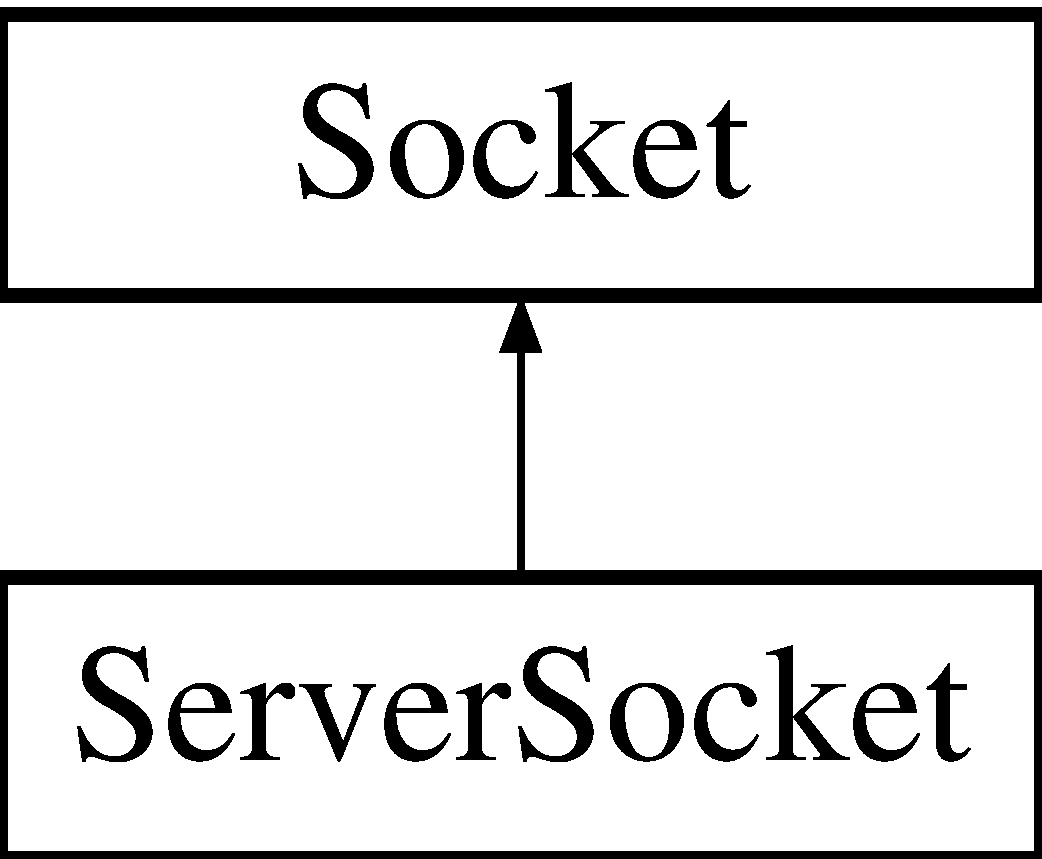
\includegraphics[height=2.000000cm]{classSocket}
\end{center}
\end{figure}
\subsection*{Public Member Functions}
\begin{DoxyCompactItemize}
\item 
\hypertarget{classSocket_a6afde2dca985dacdfa770141192e2daf}{bool {\bfseries create} ()}\label{classSocket_a6afde2dca985dacdfa770141192e2daf}

\item 
\hypertarget{classSocket_abfc7244009defd5c5e1ad173142a5059}{bool {\bfseries bind} (const int port)}\label{classSocket_abfc7244009defd5c5e1ad173142a5059}

\item 
\hypertarget{classSocket_a0988791cca0cc0eeee0c854500d7f527}{bool {\bfseries listen} () const }\label{classSocket_a0988791cca0cc0eeee0c854500d7f527}

\item 
\hypertarget{classSocket_a068f789510d289f59a1fc1f51fbb9ed3}{bool {\bfseries accept} (\hyperlink{classSocket}{Socket} \&) const }\label{classSocket_a068f789510d289f59a1fc1f51fbb9ed3}

\item 
\hypertarget{classSocket_afe535648cf44461c6ded1b2d72056d47}{bool {\bfseries connect} (const std\-::string host, const int port)}\label{classSocket_afe535648cf44461c6ded1b2d72056d47}

\item 
\hypertarget{classSocket_a011c857282aadbfde92558985e0191cd}{bool {\bfseries send} (const std\-::string) const }\label{classSocket_a011c857282aadbfde92558985e0191cd}

\item 
\hypertarget{classSocket_af6cbe662cffa8f593f9c0e42440180f3}{int {\bfseries recv} (std\-::string \&) const }\label{classSocket_af6cbe662cffa8f593f9c0e42440180f3}

\item 
\hypertarget{classSocket_ac4d1d5bc09e469b72f52fbcf758a5cf0}{void {\bfseries set\-\_\-non\-\_\-blocking} (const bool)}\label{classSocket_ac4d1d5bc09e469b72f52fbcf758a5cf0}

\item 
\hypertarget{classSocket_a157f83a7404aec259c58783cd9af6ea6}{bool {\bfseries is\-\_\-valid} () const }\label{classSocket_a157f83a7404aec259c58783cd9af6ea6}

\end{DoxyCompactItemize}


\subsection{Detailed Description}


Definition at line 20 of file Socket.\-h.



The documentation for this class was generated from the following files\-:\begin{DoxyCompactItemize}
\item 
/home/antipant/\-Protocol\-P\-\_\-\-Project/Socket.\-h\item 
/home/antipant/\-Protocol\-P\-\_\-\-Project/Socket.\-cpp\end{DoxyCompactItemize}

\hypertarget{classSocketException}{\section{Socket\-Exception Class Reference}
\label{classSocketException}\index{Socket\-Exception@{Socket\-Exception}}
}
\subsection*{Public Member Functions}
\begin{DoxyCompactItemize}
\item 
\hypertarget{classSocketException_a09ddb0c061c40fcb527ff89a2e803342}{{\bfseries Socket\-Exception} (std\-::string s)}\label{classSocketException_a09ddb0c061c40fcb527ff89a2e803342}

\item 
\hypertarget{classSocketException_ad7920caebddc99b6bbb7dbede569fa18}{std\-::string {\bfseries description} ()}\label{classSocketException_ad7920caebddc99b6bbb7dbede569fa18}

\end{DoxyCompactItemize}


\subsection{Detailed Description}


Definition at line 9 of file Socket\-Exception.\-h.



The documentation for this class was generated from the following file\-:\begin{DoxyCompactItemize}
\item 
/home/antipant/\-Protocol\-P\-\_\-\-Project/Socket\-Exception.\-h\end{DoxyCompactItemize}

\hypertarget{classtiles_1_1StateTrackingSprite}{\section{tiles.\-State\-Tracking\-Sprite Class Reference}
\label{classtiles_1_1StateTrackingSprite}\index{tiles.\-State\-Tracking\-Sprite@{tiles.\-State\-Tracking\-Sprite}}
}
Inheritance diagram for tiles.\-State\-Tracking\-Sprite\-:\begin{figure}[H]
\begin{center}
\leavevmode
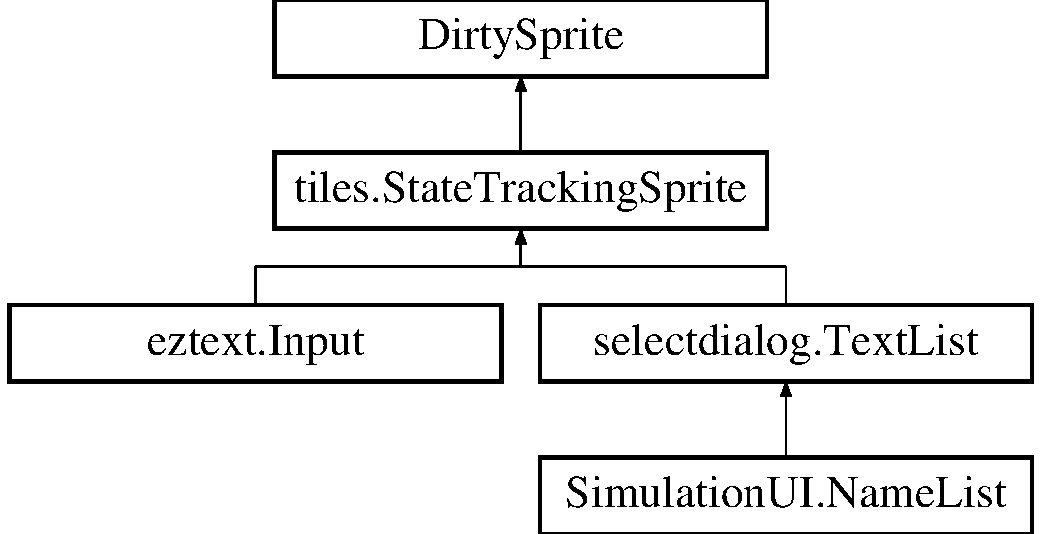
\includegraphics[height=4.000000cm]{classtiles_1_1StateTrackingSprite}
\end{center}
\end{figure}
\subsection*{Public Member Functions}
\begin{DoxyCompactItemize}
\item 
\hypertarget{classtiles_1_1StateTrackingSprite_a8ba9bb3952a9fbbc4d84bdc79c792eab}{def {\bfseries \-\_\-\-\_\-init\-\_\-\-\_\-}}\label{classtiles_1_1StateTrackingSprite_a8ba9bb3952a9fbbc4d84bdc79c792eab}

\item 
\hypertarget{classtiles_1_1StateTrackingSprite_ab53468b1c606fe0f513a1fb7cf446c63}{def {\bfseries get\-\_\-state}}\label{classtiles_1_1StateTrackingSprite_ab53468b1c606fe0f513a1fb7cf446c63}

\item 
\hypertarget{classtiles_1_1StateTrackingSprite_ad85028bf7b40f8dbd1b5e2d24185acf2}{def {\bfseries redraw}}\label{classtiles_1_1StateTrackingSprite_ad85028bf7b40f8dbd1b5e2d24185acf2}

\item 
\hypertarget{classtiles_1_1StateTrackingSprite_a72e277ca649b0f2646380ab3c8606efc}{def {\bfseries update}}\label{classtiles_1_1StateTrackingSprite_a72e277ca649b0f2646380ab3c8606efc}

\end{DoxyCompactItemize}
\subsection*{Data Fields}
\begin{DoxyCompactItemize}
\item 
\hypertarget{classtiles_1_1StateTrackingSprite_a48096bb179aaca63dbbeff68025c2b76}{{\bfseries state}}\label{classtiles_1_1StateTrackingSprite_a48096bb179aaca63dbbeff68025c2b76}

\item 
\hypertarget{classtiles_1_1StateTrackingSprite_a371c1596b332bce434ad48e7ab9312ad}{{\bfseries dirty}}\label{classtiles_1_1StateTrackingSprite_a371c1596b332bce434ad48e7ab9312ad}

\end{DoxyCompactItemize}


\subsection{Detailed Description}


Definition at line 61 of file tiles.\-py.



The documentation for this class was generated from the following file\-:\begin{DoxyCompactItemize}
\item 
/home/antipant/\-Protocol\-P\-\_\-\-Project/\-U\-I/tiles.\-py\end{DoxyCompactItemize}

\hypertarget{classtiles_1_1StaticSprite}{\section{tiles.\-Static\-Sprite Class Reference}
\label{classtiles_1_1StaticSprite}\index{tiles.\-Static\-Sprite@{tiles.\-Static\-Sprite}}
}
Inheritance diagram for tiles.\-Static\-Sprite\-:\begin{figure}[H]
\begin{center}
\leavevmode
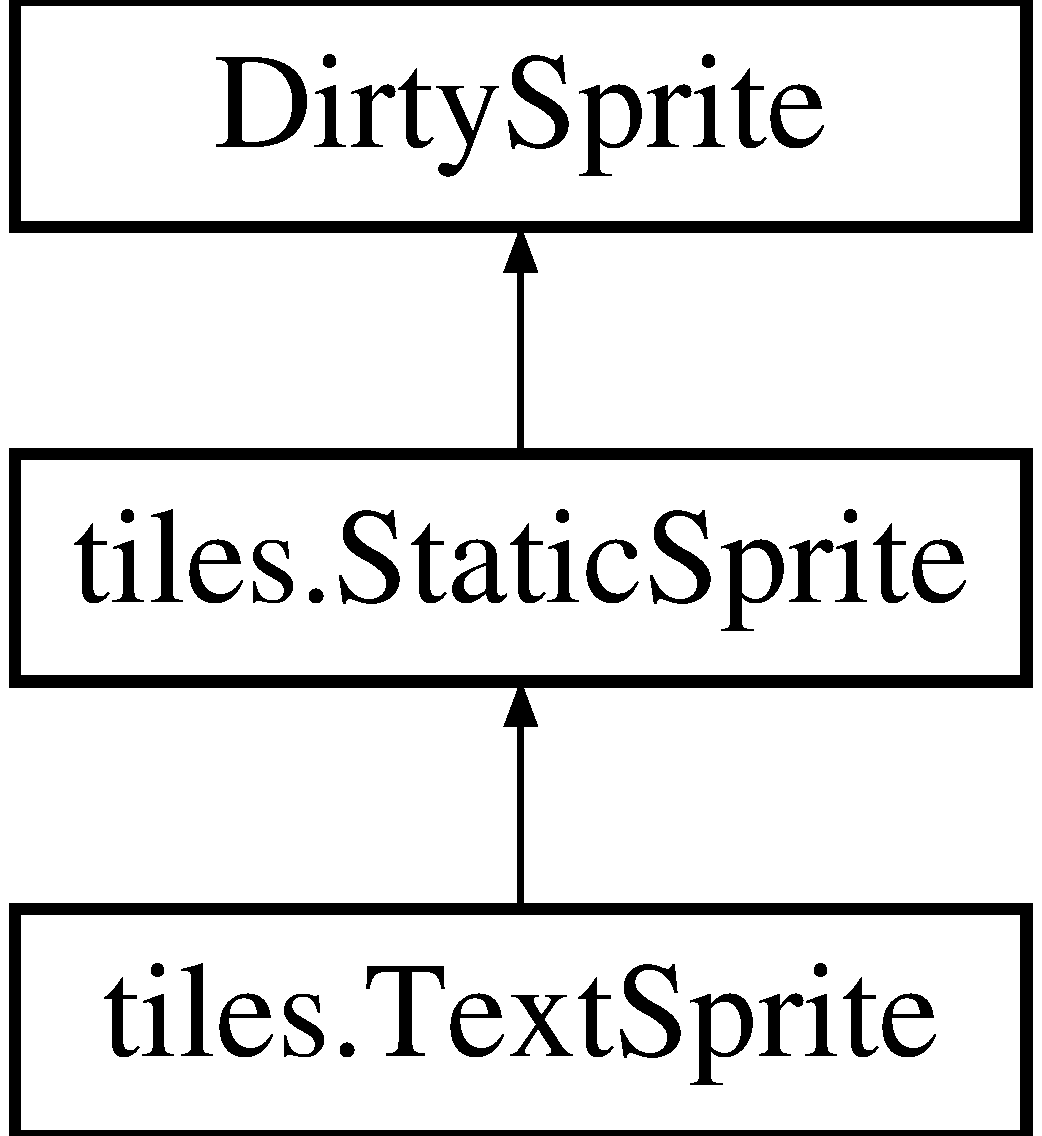
\includegraphics[height=3.000000cm]{classtiles_1_1StaticSprite}
\end{center}
\end{figure}
\subsection*{Public Member Functions}
\begin{DoxyCompactItemize}
\item 
\hypertarget{classtiles_1_1StaticSprite_af23e7a9b77408f4ac429cc680cdb74d6}{def {\bfseries \-\_\-\-\_\-init\-\_\-\-\_\-}}\label{classtiles_1_1StaticSprite_af23e7a9b77408f4ac429cc680cdb74d6}

\end{DoxyCompactItemize}
\subsection*{Data Fields}
\begin{DoxyCompactItemize}
\item 
\hypertarget{classtiles_1_1StaticSprite_a09114e04f50b1dec8525af745f8e34b9}{{\bfseries image}}\label{classtiles_1_1StaticSprite_a09114e04f50b1dec8525af745f8e34b9}

\item 
\hypertarget{classtiles_1_1StaticSprite_a4cd5482f618aeb1c835c120e0ea4fcea}{{\bfseries rect}}\label{classtiles_1_1StaticSprite_a4cd5482f618aeb1c835c120e0ea4fcea}

\end{DoxyCompactItemize}


\subsection{Detailed Description}


Definition at line 4 of file tiles.\-py.



The documentation for this class was generated from the following file\-:\begin{DoxyCompactItemize}
\item 
/home/antipant/\-Protocol\-P\-\_\-\-Project/\-U\-I/tiles.\-py\end{DoxyCompactItemize}

\hypertarget{classStringTool}{\section{String\-Tool Class Reference}
\label{classStringTool}\index{String\-Tool@{String\-Tool}}
}


The documentation for this class was generated from the following file\-:\begin{DoxyCompactItemize}
\item 
/home/antipant/\-Protocol\-P\-\_\-\-Project/\hyperlink{StringTools_8hpp}{String\-Tools.\-hpp}\end{DoxyCompactItemize}

\hypertarget{classStringTools}{\section{String\-Tools Class Reference}
\label{classStringTools}\index{String\-Tools@{String\-Tools}}
}
\subsection*{Public Member Functions}
\begin{DoxyCompactItemize}
\item 
\hypertarget{classStringTools_ad0ce8a471ba7eb6e48a8609ab924d1d5}{{\bfseries String\-Tools} (string p\-\_\-\-Base\-Name)}\label{classStringTools_ad0ce8a471ba7eb6e48a8609ab924d1d5}

\item 
\hypertarget{classStringTools_a3ff5ab3693687b6359003b7246a02283}{{\bfseries String\-Tools} (string p\-\_\-\-Base\-Name, string p\-\_\-\-Separator)}\label{classStringTools_a3ff5ab3693687b6359003b7246a02283}

\item 
\hypertarget{classStringTools_aa42f8614db6be692ea5186874b66009c}{{\bfseries String\-Tools} (const char $\ast$p\-\_\-\-Base\-Name)}\label{classStringTools_aa42f8614db6be692ea5186874b66009c}

\item 
\hypertarget{classStringTools_a9b9003e1e4a696edd5c4cb1c84e6d11c}{{\bfseries String\-Tools} (const char $\ast$p\-\_\-\-Base\-Name, bool p\-\_\-\-Stamp\-Time)}\label{classStringTools_a9b9003e1e4a696edd5c4cb1c84e6d11c}

\item 
\hypertarget{classStringTools_a0ce4f82e772571fc12577eb9f1691e06}{void {\bfseries set\-Base\-Name} (string p\-\_\-\-Base\-Name)}\label{classStringTools_a0ce4f82e772571fc12577eb9f1691e06}

\item 
\hypertarget{classStringTools_a272d76e82bdfe029acbf0bd65744025d}{const char $\ast$ {\bfseries get\-Next\-Name} (void)}\label{classStringTools_a272d76e82bdfe029acbf0bd65744025d}

\item 
\hypertarget{classStringTools_a0d352e612af5b42b3324de44baaeeec9}{const char $\ast$ {\bfseries get\-Current\-Name} (void)}\label{classStringTools_a0d352e612af5b42b3324de44baaeeec9}

\item 
\hypertarget{classStringTools_a498868ff22278d1be842ad92be7b3e52}{void {\bfseries reset\-Identifier} (void)}\label{classStringTools_a498868ff22278d1be842ad92be7b3e52}

\item 
\hypertarget{classStringTools_a673dcdaa425b6e08d24dadebbbb819a6}{void {\bfseries set\-Identifier} (int p\-\_\-\-Identifier)}\label{classStringTools_a673dcdaa425b6e08d24dadebbbb819a6}

\item 
\hypertarget{classStringTools_a7c53fe0bee5863c8a60fd00de8ee31cd}{void {\bfseries set\-Separator} (string p\-\_\-\-Separator)}\label{classStringTools_a7c53fe0bee5863c8a60fd00de8ee31cd}

\item 
\hypertarget{classStringTools_a5ad25d9ce230ceb78f9de0fd265c0eda}{void {\bfseries set\-Stamp\-Time} (bool p\-\_\-\-Stamp\-Time)}\label{classStringTools_a5ad25d9ce230ceb78f9de0fd265c0eda}

\item 
\hypertarget{classStringTools_a9c6cfac09aa84ede205615484adc6fef}{void {\bfseries set\-Reset} (bool p\-\_\-\-Reset)}\label{classStringTools_a9c6cfac09aa84ede205615484adc6fef}

\item 
\hypertarget{classStringTools_a47594cf2ed9755da81c1ac31afb531ed}{void {\bfseries append\-String} (const char $\ast$p\-\_\-\-Report\-String)}\label{classStringTools_a47594cf2ed9755da81c1ac31afb531ed}

\item 
\hypertarget{classStringTools_a726e754e512e5515678de7a9f72f7968}{const char $\ast$ {\bfseries get\-Report\-String} (void)}\label{classStringTools_a726e754e512e5515678de7a9f72f7968}

\item 
\hypertarget{classStringTools_a87cc25f9580e48c998495995280ebe7b}{const char $\ast$ {\bfseries new\-Report\-String} (const char $\ast$p\-\_\-\-Report\-String)}\label{classStringTools_a87cc25f9580e48c998495995280ebe7b}

\item 
\hypertarget{classStringTools_a57cb7b0268c5ef8fa1f3ab64f3fab974}{const char $\ast$ {\bfseries new\-Report\-String} (string p\-\_\-\-Report\-String)}\label{classStringTools_a57cb7b0268c5ef8fa1f3ab64f3fab974}

\item 
\hypertarget{classStringTools_a637a5d56f642802d896b9e57d081889d}{const char $\ast$ {\bfseries append\-Report\-String} (const char $\ast$p\-\_\-\-Report\-String)}\label{classStringTools_a637a5d56f642802d896b9e57d081889d}

\item 
\hypertarget{classStringTools_a452c24f683db8caa4837bc8190b7208d}{const char $\ast$ {\bfseries append\-Report\-String} (string p\-\_\-\-Report\-String)}\label{classStringTools_a452c24f683db8caa4837bc8190b7208d}

\item 
\hypertarget{classStringTools_aec710716ef3d9cff807fd70c7d848d33}{const char $\ast$ {\bfseries new\-Report\-String} (int p\-\_\-\-Report\-Int)}\label{classStringTools_aec710716ef3d9cff807fd70c7d848d33}

\item 
\hypertarget{classStringTools_ad4fdc3dc36b9b7f25f794330ffee2047}{const char $\ast$ {\bfseries append\-Report\-String} (int p\-\_\-\-Report\-Int)}\label{classStringTools_ad4fdc3dc36b9b7f25f794330ffee2047}

\item 
\hypertarget{classStringTools_ae0b98503fca8fdb3d5a3eac77f203839}{void {\bfseries reset\-Report\-String} (void)}\label{classStringTools_ae0b98503fca8fdb3d5a3eac77f203839}

\item 
\hypertarget{classStringTools_a142900b271efdee814d71239de643eba}{string {\bfseries i\-To\-S} (int p\-\_\-\-Value)}\label{classStringTools_a142900b271efdee814d71239de643eba}

\item 
\hypertarget{classStringTools_ac2126c3eec7acef09f8fd46291b2413e}{string {\bfseries u\-To\-S} (unsigned p\-\_\-\-Value)}\label{classStringTools_ac2126c3eec7acef09f8fd46291b2413e}

\item 
\hypertarget{classStringTools_a50b5f1a75109971e60d6543ee76816fc}{int {\bfseries s\-To\-I} (string p\-\_\-\-Value)}\label{classStringTools_a50b5f1a75109971e60d6543ee76816fc}

\item 
\hypertarget{classStringTools_a5627021cfdc5e0586aa31d4cce7fab17}{unsigned {\bfseries s\-To\-U} (string p\-\_\-\-Value)}\label{classStringTools_a5627021cfdc5e0586aa31d4cce7fab17}

\item 
\hypertarget{classStringTools_a23c0ef7bac00175a378a75ca7a07bb41}{sc\-\_\-uint$<$ 32 $>$ {\bfseries convert\-I\-P\-To\-Binary} (string p\-\_\-\-Prefix)}\label{classStringTools_a23c0ef7bac00175a378a75ca7a07bb41}

\item 
\hypertarget{classStringTools_a9395eb0395c837334067f4d24527b5a1}{sc\-\_\-uint$<$ 32 $>$ {\bfseries convert\-Mask\-To\-Binary} (string p\-\_\-\-Prefix)}\label{classStringTools_a9395eb0395c837334067f4d24527b5a1}

\item 
\hypertarget{classStringTools_ac9bdf54d89ba0512e692e4a8c7567bb4}{string {\bfseries convert\-I\-P\-To\-String} (sc\-\_\-uint$<$ 32 $>$ p\-\_\-\-I\-P, sc\-\_\-uint$<$ 32 $>$ p\-\_\-\-Mask)}\label{classStringTools_ac9bdf54d89ba0512e692e4a8c7567bb4}

\item 
\hypertarget{classStringTools_a2007d59fec97ffdc06f13d415d26aabf}{string {\bfseries convert\-I\-P\-To\-String} (sc\-\_\-uint$<$ 32 $>$ p\-\_\-\-I\-P)}\label{classStringTools_a2007d59fec97ffdc06f13d415d26aabf}

\item 
\hypertarget{classStringTools_a4d8b34eea1fe2d6d1832a197ac359d01}{string {\bfseries convert\-Mask\-To\-String} (sc\-\_\-uint$<$ 32 $>$ p\-\_\-\-Mask)}\label{classStringTools_a4d8b34eea1fe2d6d1832a197ac359d01}

\item 
\hypertarget{classStringTools_a76d91a24ce92b5cee2d6241beaacb037}{string {\bfseries set\-I\-P\-Low\-Octet} (string p\-\_\-\-I\-P, unsigned char p\-\_\-\-Value)}\label{classStringTools_a76d91a24ce92b5cee2d6241beaacb037}

\item 
bool \hyperlink{classStringTools_a833132f86813cb0f8a65b748d12e8d9b}{ip\-To\-U\-Char} (string p\-\_\-\-I\-P\-Address, unsigned char $\ast$p\-\_\-\-I\-P\-Bin\-Address)
\begin{DoxyCompactList}\small\item\em Converts string type I\-P\-Address to binary form in four element unsigned char array. \end{DoxyCompactList}\item 
string \hyperlink{classStringTools_a65c8cae22cd041ff3e5053a6f0d7c5b5}{ip\-To\-String} (unsigned char $\ast$ptr\-\_\-\-I\-P\-Bin\-Address)
\begin{DoxyCompactList}\small\item\em Converts I\-P address from four byte binary form to string form. \end{DoxyCompactList}\end{DoxyCompactItemize}


\subsection{Detailed Description}


Definition at line 25 of file String\-Tools.\-hpp.



\subsection{Member Function Documentation}
\hypertarget{classStringTools_a65c8cae22cd041ff3e5053a6f0d7c5b5}{\index{String\-Tools@{String\-Tools}!ip\-To\-String@{ip\-To\-String}}
\index{ip\-To\-String@{ip\-To\-String}!StringTools@{String\-Tools}}
\subsubsection[{ip\-To\-String}]{\setlength{\rightskip}{0pt plus 5cm}string String\-Tools\-::ip\-To\-String (
\begin{DoxyParamCaption}
\item[{unsigned char $\ast$}]{ptr\-\_\-\-I\-P\-Bin\-Address}
\end{DoxyParamCaption}
)}}\label{classStringTools_a65c8cae22cd041ff3e5053a6f0d7c5b5}


Converts I\-P address from four byte binary form to string form. 

\begin{DoxySeeAlso}{See Also}
\hyperlink{classStringTools}{String\-Tools}
\end{DoxySeeAlso}

\begin{DoxyParams}[1]{Parameters}
\mbox{\tt in}  & {\em unsigned} & p\-\_\-\-I\-P\-Bin\-Address The ip address in binary form \\
\hline
\end{DoxyParams}
\begin{DoxyReturn}{Returns}
string\-: The I\-P address in string 
\end{DoxyReturn}


Definition at line 322 of file String\-Tools.\-cpp.

\hypertarget{classStringTools_a833132f86813cb0f8a65b748d12e8d9b}{\index{String\-Tools@{String\-Tools}!ip\-To\-U\-Char@{ip\-To\-U\-Char}}
\index{ip\-To\-U\-Char@{ip\-To\-U\-Char}!StringTools@{String\-Tools}}
\subsubsection[{ip\-To\-U\-Char}]{\setlength{\rightskip}{0pt plus 5cm}bool String\-Tools\-::ip\-To\-U\-Char (
\begin{DoxyParamCaption}
\item[{string}]{p\-\_\-\-I\-P\-Address, }
\item[{unsigned char $\ast$}]{p\-\_\-\-I\-P\-Bin\-Address}
\end{DoxyParamCaption}
)}}\label{classStringTools_a833132f86813cb0f8a65b748d12e8d9b}


Converts string type I\-P\-Address to binary form in four element unsigned char array. 

\begin{DoxySeeAlso}{See Also}
\hyperlink{classStringTools}{String\-Tools}
\end{DoxySeeAlso}

\begin{DoxyParams}[1]{Parameters}
\mbox{\tt in}  & {\em string} & p\-\_\-\-I\-P\-Address \\
\hline
\mbox{\tt out}  & {\em unsigned} & char $\ast$p\-\_\-\-I\-P\-Bin\-Address \\
\hline
\end{DoxyParams}
\begin{DoxyReturn}{Returns}
bool\-: true -\/ conversion success $|$ false -\/ conversion failed 
\end{DoxyReturn}


Definition at line 280 of file String\-Tools.\-cpp.



The documentation for this class was generated from the following files\-:\begin{DoxyCompactItemize}
\item 
/home/antipant/\-Protocol\-P\-\_\-\-Project/\hyperlink{StringTools_8hpp}{String\-Tools.\-hpp}\item 
/home/antipant/\-Protocol\-P\-\_\-\-Project/String\-Tools.\-cpp\end{DoxyCompactItemize}

\hypertarget{structstruct__Route}{\section{struct\-\_\-\-Route Struct Reference}
\label{structstruct__Route}\index{struct\-\_\-\-Route@{struct\-\_\-\-Route}}
}
\subsection*{Data Fields}
\begin{DoxyCompactItemize}
\item 
\hypertarget{structstruct__Route_a3dff90ab63fcc429ca80a3ef8ef3ad48}{int {\bfseries id}}\label{structstruct__Route_a3dff90ab63fcc429ca80a3ef8ef3ad48}

\item 
\hypertarget{structstruct__Route_aa37611b878f02a5b6dd235010dff0656}{string {\bfseries prefix}}\label{structstruct__Route_aa37611b878f02a5b6dd235010dff0656}

\item 
\hypertarget{structstruct__Route_a686f4a523cc70a19ba1725676b7a281e}{int {\bfseries mask}}\label{structstruct__Route_a686f4a523cc70a19ba1725676b7a281e}

\item 
\hypertarget{structstruct__Route_aa701995db61b15b8218cd649a2e1f062}{string {\bfseries A\-Ses}}\label{structstruct__Route_aa701995db61b15b8218cd649a2e1f062}

\item 
\hypertarget{structstruct__Route_a45a03fa95a6c99b6c232befd759effce}{int {\bfseries Output\-Port}}\label{structstruct__Route_a45a03fa95a6c99b6c232befd759effce}

\item 
\hypertarget{structstruct__Route_ab3531db9abe6c0ca498ed592919c0cc7}{\hyperlink{structstruct__Route}{struct\-\_\-\-Route} $\ast$ {\bfseries next}}\label{structstruct__Route_ab3531db9abe6c0ca498ed592919c0cc7}

\end{DoxyCompactItemize}


\subsection{Detailed Description}


Definition at line 36 of file Routing\-Table.\-hpp.



The documentation for this struct was generated from the following file\-:\begin{DoxyCompactItemize}
\item 
/home/antipant/\-Protocol\-P\-\_\-\-Project/\hyperlink{RoutingTable_8hpp}{Routing\-Table.\-hpp}\end{DoxyCompactItemize}

\hypertarget{classselectdialog_1_1TextList}{\section{selectdialog.\-Text\-List Class Reference}
\label{classselectdialog_1_1TextList}\index{selectdialog.\-Text\-List@{selectdialog.\-Text\-List}}
}
Inheritance diagram for selectdialog.\-Text\-List\-:\begin{figure}[H]
\begin{center}
\leavevmode
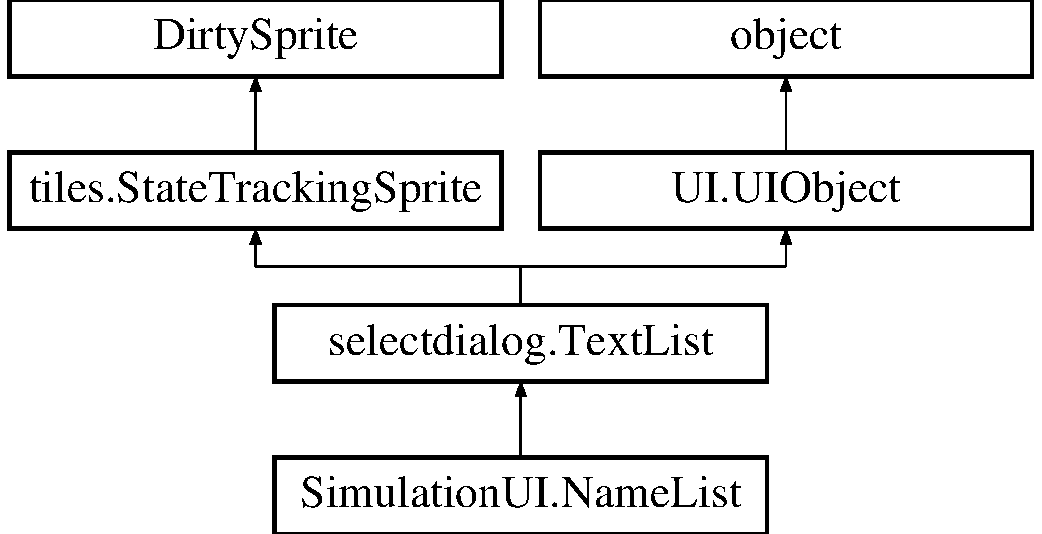
\includegraphics[height=4.000000cm]{classselectdialog_1_1TextList}
\end{center}
\end{figure}
\subsection*{Public Member Functions}
\begin{DoxyCompactItemize}
\item 
\hypertarget{classselectdialog_1_1TextList_a64c584b530d7829d9eba5287d807cd13}{def {\bfseries \-\_\-\-\_\-init\-\_\-\-\_\-}}\label{classselectdialog_1_1TextList_a64c584b530d7829d9eba5287d807cd13}

\item 
\hypertarget{classselectdialog_1_1TextList_ac1f4e713d0473dbba99ba82674947161}{def {\bfseries event}}\label{classselectdialog_1_1TextList_ac1f4e713d0473dbba99ba82674947161}

\item 
\hypertarget{classselectdialog_1_1TextList_a74de44978d0ae55c6d7ec62c4ce4b027}{def {\bfseries get\-\_\-state}}\label{classselectdialog_1_1TextList_a74de44978d0ae55c6d7ec62c4ce4b027}

\item 
\hypertarget{classselectdialog_1_1TextList_a950b9c0303d2c564926a8b6c30e58aa9}{def {\bfseries redraw}}\label{classselectdialog_1_1TextList_a950b9c0303d2c564926a8b6c30e58aa9}

\item 
\hypertarget{classselectdialog_1_1TextList_a5e99de791bb502fbb15f867ad520b60b}{def {\bfseries format\-\_\-item}}\label{classselectdialog_1_1TextList_a5e99de791bb502fbb15f867ad520b60b}

\item 
\hypertarget{classselectdialog_1_1TextList_ac69606b47a872b4dcda0f8d34bde9225}{def {\bfseries selected}}\label{classselectdialog_1_1TextList_ac69606b47a872b4dcda0f8d34bde9225}

\item 
\hypertarget{classselectdialog_1_1TextList_ab31b27c42622b998fed479848f777cb3}{def {\bfseries get\-\_\-selected}}\label{classselectdialog_1_1TextList_ab31b27c42622b998fed479848f777cb3}

\item 
\hypertarget{classselectdialog_1_1TextList_a3b69f3a018755c286f44b4cf66ae01d4}{def {\bfseries get\-\_\-selected\-\_\-item}}\label{classselectdialog_1_1TextList_a3b69f3a018755c286f44b4cf66ae01d4}

\item 
\hypertarget{classselectdialog_1_1TextList_a0a3d33200f5507492d6da3697f352969}{def {\bfseries remove\-\_\-at}}\label{classselectdialog_1_1TextList_a0a3d33200f5507492d6da3697f352969}

\item 
\hypertarget{classselectdialog_1_1TextList_ab9bff5a624c27421582edc7e747374e6}{def {\bfseries remove}}\label{classselectdialog_1_1TextList_ab9bff5a624c27421582edc7e747374e6}

\item 
\hypertarget{classselectdialog_1_1TextList_ad08394e14f3ec0228e0cda00320266a2}{def {\bfseries replace}}\label{classselectdialog_1_1TextList_ad08394e14f3ec0228e0cda00320266a2}

\end{DoxyCompactItemize}
\subsection*{Data Fields}
\begin{DoxyCompactItemize}
\item 
\hypertarget{classselectdialog_1_1TextList_a1cc5e1811bcb1d1b45d3a9b37b1faf62}{{\bfseries image}}\label{classselectdialog_1_1TextList_a1cc5e1811bcb1d1b45d3a9b37b1faf62}

\item 
\hypertarget{classselectdialog_1_1TextList_aa47290b84869a0c9ee3e685c2e8eea7b}{{\bfseries font}}\label{classselectdialog_1_1TextList_aa47290b84869a0c9ee3e685c2e8eea7b}

\item 
\hypertarget{classselectdialog_1_1TextList_a0ca9553b8e9499c80f4486b3d8381430}{{\bfseries linesize}}\label{classselectdialog_1_1TextList_a0ca9553b8e9499c80f4486b3d8381430}

\item 
\hypertarget{classselectdialog_1_1TextList_af6c871de008b4d8637872a49bd100024}{{\bfseries linecount}}\label{classselectdialog_1_1TextList_af6c871de008b4d8637872a49bd100024}

\item 
\hypertarget{classselectdialog_1_1TextList_a6ceb11c44ba027c63d3981d53acd7ca6}{{\bfseries tickless}}\label{classselectdialog_1_1TextList_a6ceb11c44ba027c63d3981d53acd7ca6}

\item 
\hypertarget{classselectdialog_1_1TextList_a8f37113ee413e9dfa199d50a724e2986}{{\bfseries ratios}}\label{classselectdialog_1_1TextList_a8f37113ee413e9dfa199d50a724e2986}

\item 
\hypertarget{classselectdialog_1_1TextList_a039dcaefbbca4ff89155e49c8473845f}{{\bfseries items}}\label{classselectdialog_1_1TextList_a039dcaefbbca4ff89155e49c8473845f}

\item 
\hypertarget{classselectdialog_1_1TextList_a3c5c1d66606acea5caab4320ccaf0271}{{\bfseries multi}}\label{classselectdialog_1_1TextList_a3c5c1d66606acea5caab4320ccaf0271}

\item 
\hypertarget{classselectdialog_1_1TextList_ad57a076770a899c9cf8ea562a97fa768}{{\bfseries sel}}\label{classselectdialog_1_1TextList_ad57a076770a899c9cf8ea562a97fa768}

\item 
\hypertarget{classselectdialog_1_1TextList_aca55f2c104f2d793d42cb0e4283d88f5}{{\bfseries scroll}}\label{classselectdialog_1_1TextList_aca55f2c104f2d793d42cb0e4283d88f5}

\item 
\hypertarget{classselectdialog_1_1TextList_ac8fe19bd5e151330e82795a5e3bc4aec}{{\bfseries format\-\_\-item}}\label{classselectdialog_1_1TextList_ac8fe19bd5e151330e82795a5e3bc4aec}

\end{DoxyCompactItemize}
\subsection*{Additional Inherited Members}


\subsection{Detailed Description}


Definition at line 137 of file selectdialog.\-py.



The documentation for this class was generated from the following file\-:\begin{DoxyCompactItemize}
\item 
/home/antipant/\-Protocol\-P\-\_\-\-Project/\-U\-I/selectdialog.\-py\end{DoxyCompactItemize}

\hypertarget{classtiles_1_1TextSprite}{\section{tiles.\-Text\-Sprite Class Reference}
\label{classtiles_1_1TextSprite}\index{tiles.\-Text\-Sprite@{tiles.\-Text\-Sprite}}
}
Inheritance diagram for tiles.\-Text\-Sprite\-:\begin{figure}[H]
\begin{center}
\leavevmode
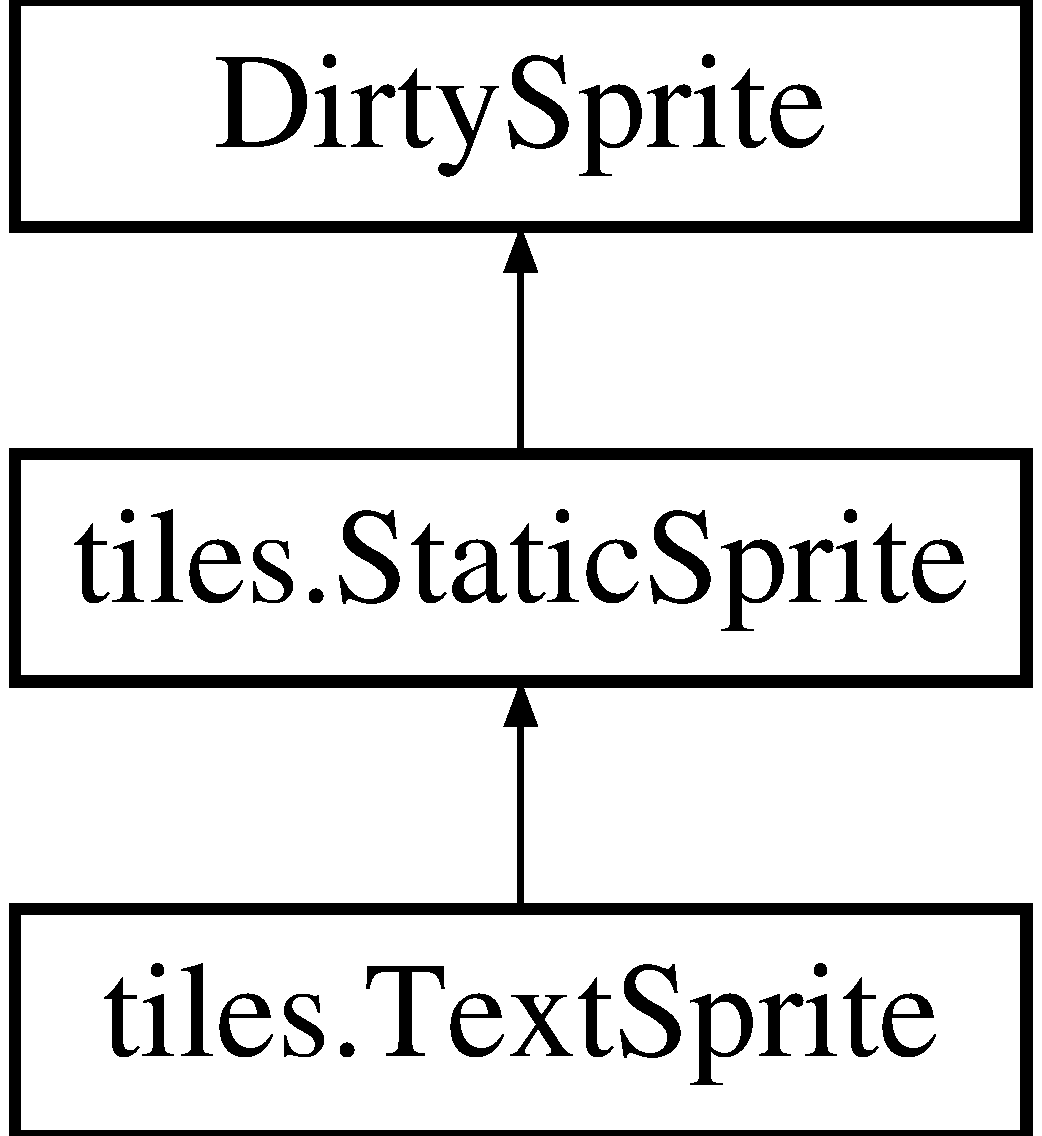
\includegraphics[height=3.000000cm]{classtiles_1_1TextSprite}
\end{center}
\end{figure}
\subsection*{Additional Inherited Members}


\subsection{Detailed Description}


Definition at line 13 of file tiles.\-py.



The documentation for this class was generated from the following file\-:\begin{DoxyCompactItemize}
\item 
/home/antipant/\-Protocol\-P\-\_\-\-Project/\-U\-I/tiles.\-py\end{DoxyCompactItemize}

\hypertarget{classUI_1_1Tile}{\section{U\-I.\-Tile Class Reference}
\label{classUI_1_1Tile}\index{U\-I.\-Tile@{U\-I.\-Tile}}
}
Inheritance diagram for U\-I.\-Tile\-:\begin{figure}[H]
\begin{center}
\leavevmode
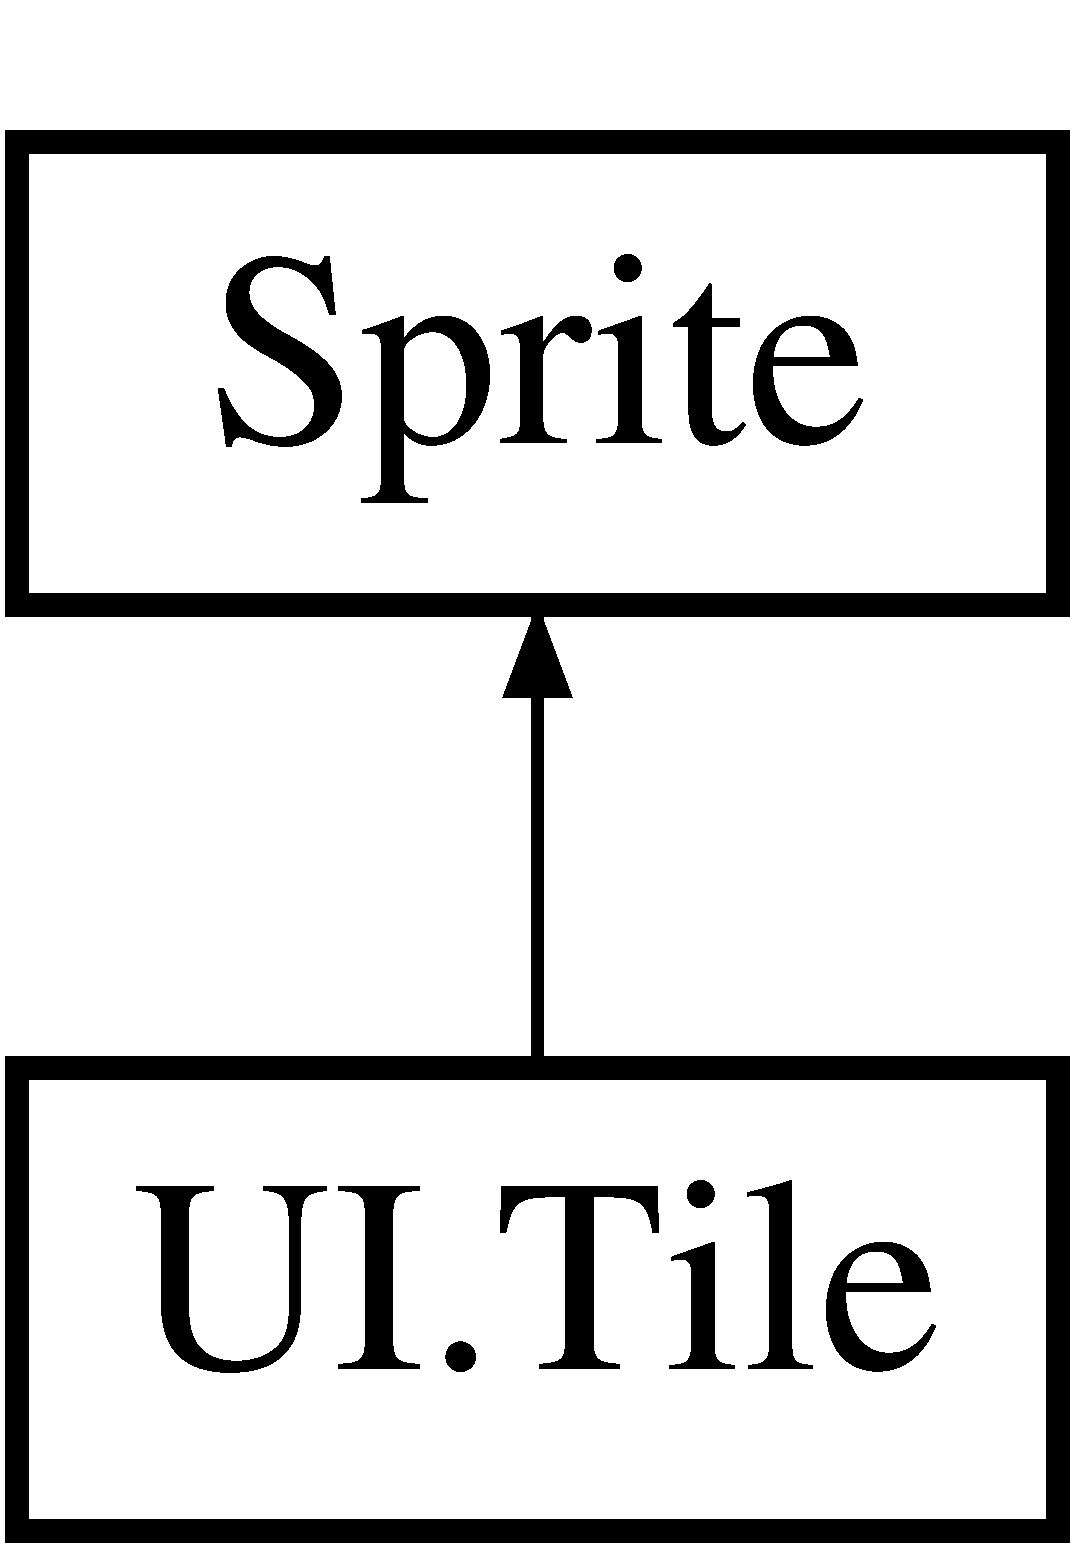
\includegraphics[height=2.000000cm]{classUI_1_1Tile}
\end{center}
\end{figure}
\subsection*{Public Member Functions}
\begin{DoxyCompactItemize}
\item 
\hypertarget{classUI_1_1Tile_a1c4f05ed21232b62e032fa41af69b982}{def {\bfseries \-\_\-\-\_\-init\-\_\-\-\_\-}}\label{classUI_1_1Tile_a1c4f05ed21232b62e032fa41af69b982}

\end{DoxyCompactItemize}
\subsection*{Data Fields}
\begin{DoxyCompactItemize}
\item 
\hypertarget{classUI_1_1Tile_a51940c7163d4bc065beeadaf4cac09e1}{{\bfseries image}}\label{classUI_1_1Tile_a51940c7163d4bc065beeadaf4cac09e1}

\item 
\hypertarget{classUI_1_1Tile_a79aeac4554e05d4d7898ea9ef18eff59}{{\bfseries rect}}\label{classUI_1_1Tile_a79aeac4554e05d4d7898ea9ef18eff59}

\end{DoxyCompactItemize}


\subsection{Detailed Description}


Definition at line 169 of file U\-I.\-py.



The documentation for this class was generated from the following file\-:\begin{DoxyCompactItemize}
\item 
/home/antipant/\-Protocol\-P\-\_\-\-Project/\-U\-I/U\-I.\-py\end{DoxyCompactItemize}

\hypertarget{classtimeout_1_1TimeoutError}{\section{timeout.\-Timeout\-Error Class Reference}
\label{classtimeout_1_1TimeoutError}\index{timeout.\-Timeout\-Error@{timeout.\-Timeout\-Error}}
}
Inheritance diagram for timeout.\-Timeout\-Error\-:\begin{figure}[H]
\begin{center}
\leavevmode
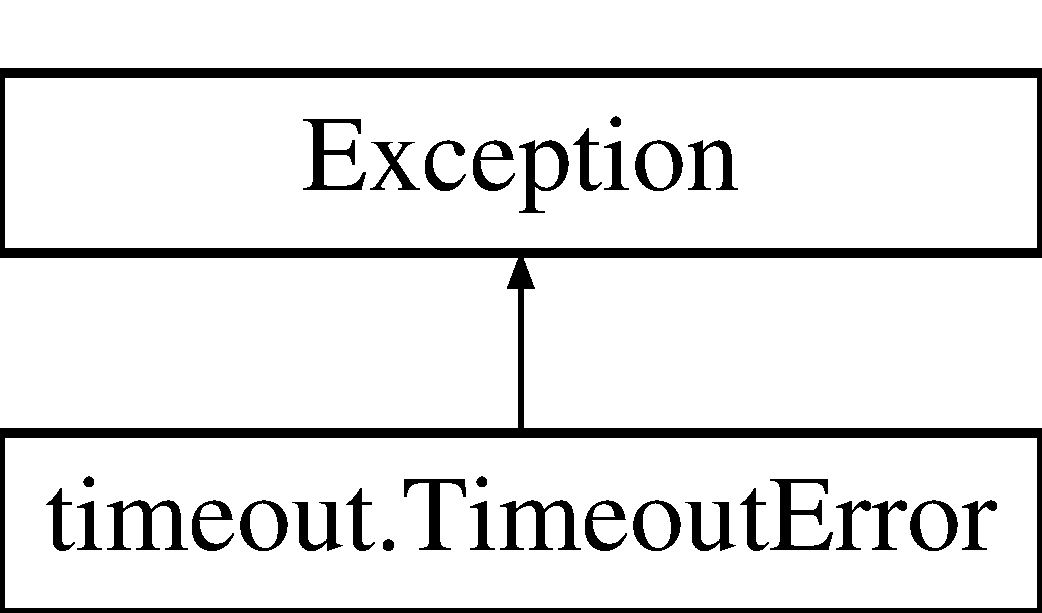
\includegraphics[height=2.000000cm]{classtimeout_1_1TimeoutError}
\end{center}
\end{figure}


\subsection{Detailed Description}


Definition at line 6 of file timeout.\-py.



The documentation for this class was generated from the following file\-:\begin{DoxyCompactItemize}
\item 
/home/antipant/\-Protocol\-P\-\_\-\-Project/\-U\-I/timeout.\-py\end{DoxyCompactItemize}

\hypertarget{classUI_1_1UIComponent}{\section{U\-I.\-U\-I\-Component Class Reference}
\label{classUI_1_1UIComponent}\index{U\-I.\-U\-I\-Component@{U\-I.\-U\-I\-Component}}
}
Inheritance diagram for U\-I.\-U\-I\-Component\-:\begin{figure}[H]
\begin{center}
\leavevmode
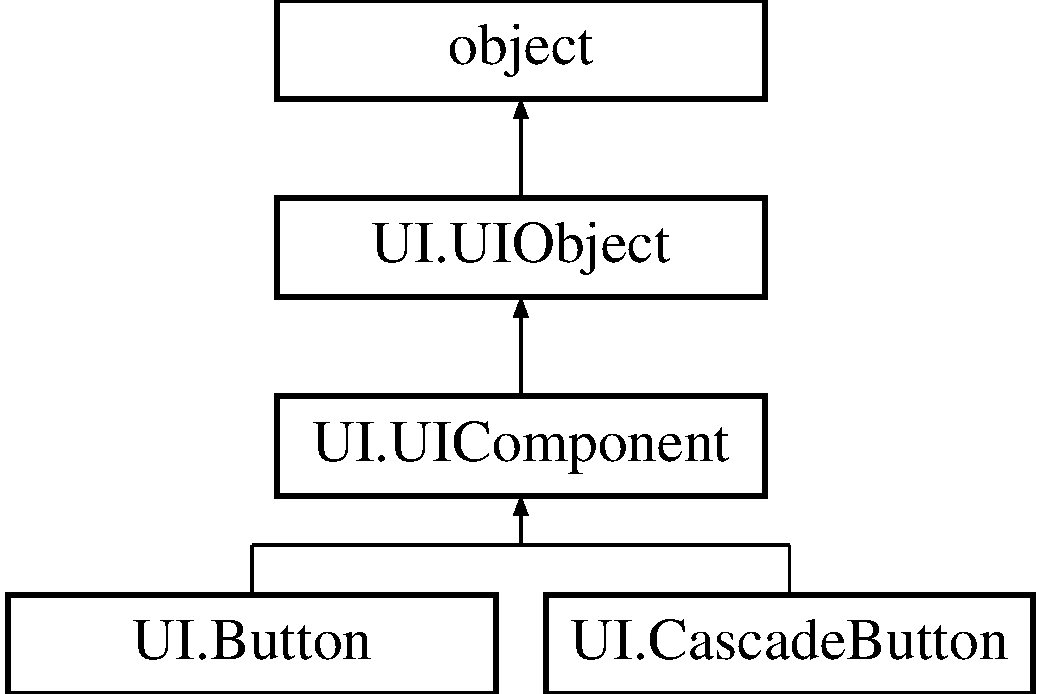
\includegraphics[height=4.000000cm]{classUI_1_1UIComponent}
\end{center}
\end{figure}
\subsection*{Public Member Functions}
\begin{DoxyCompactItemize}
\item 
\hypertarget{classUI_1_1UIComponent_a8c0d5fe4e1f297409fa4cc257c088457}{def {\bfseries \-\_\-\-\_\-init\-\_\-\-\_\-}}\label{classUI_1_1UIComponent_a8c0d5fe4e1f297409fa4cc257c088457}

\end{DoxyCompactItemize}
\subsection*{Additional Inherited Members}


\subsection{Detailed Description}


Definition at line 165 of file U\-I.\-py.



The documentation for this class was generated from the following file\-:\begin{DoxyCompactItemize}
\item 
/home/antipant/\-Protocol\-P\-\_\-\-Project/\-U\-I/U\-I.\-py\end{DoxyCompactItemize}

\hypertarget{classUI_1_1UIContainer}{\section{U\-I.\-U\-I\-Container Class Reference}
\label{classUI_1_1UIContainer}\index{U\-I.\-U\-I\-Container@{U\-I.\-U\-I\-Container}}
}
Inheritance diagram for U\-I.\-U\-I\-Container\-:\begin{figure}[H]
\begin{center}
\leavevmode
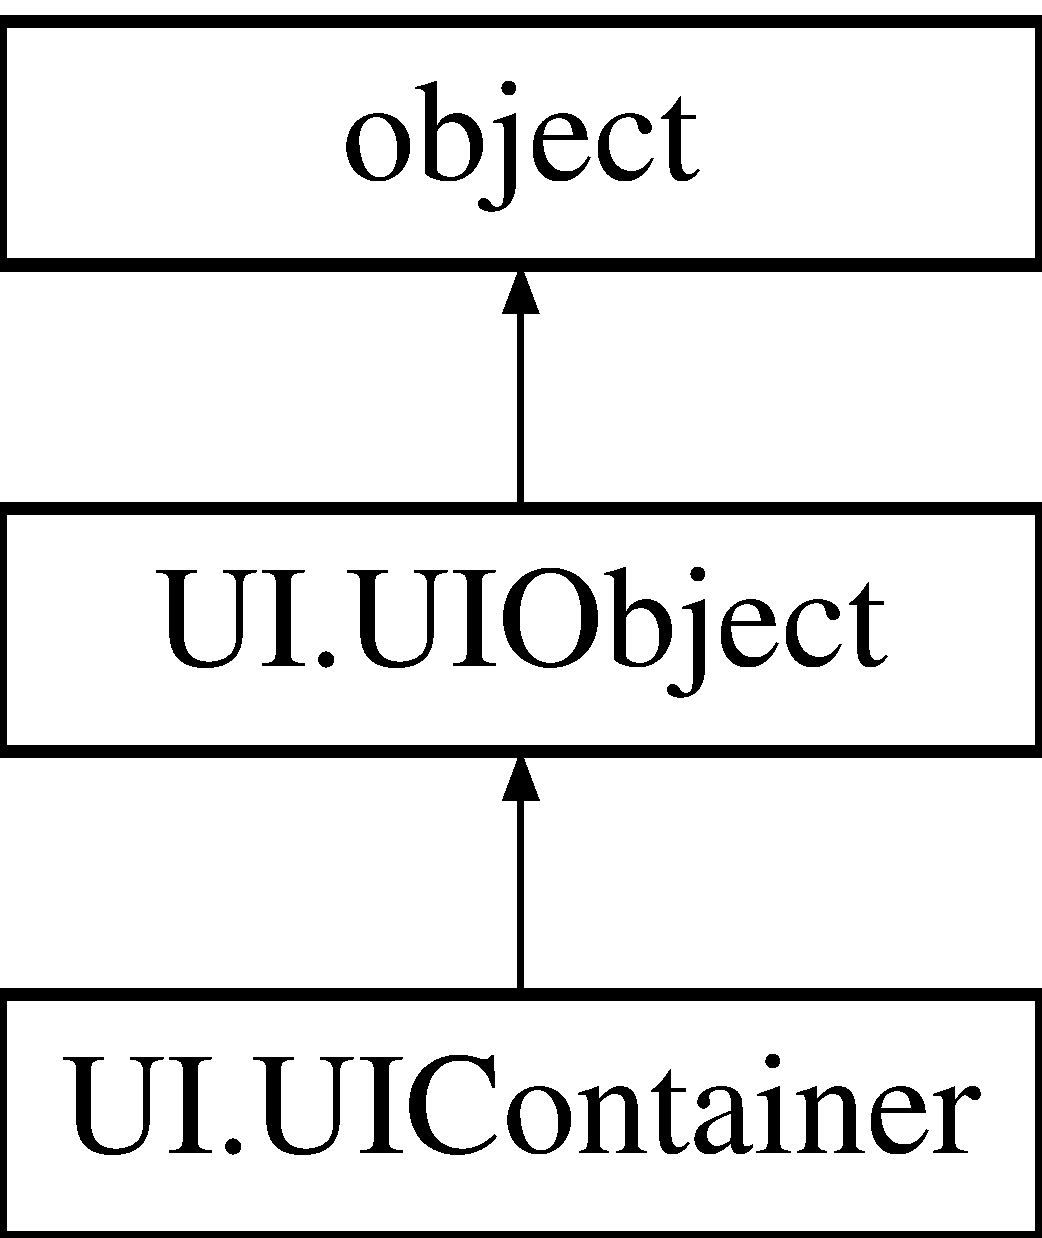
\includegraphics[height=3.000000cm]{classUI_1_1UIContainer}
\end{center}
\end{figure}
\subsection*{Public Member Functions}
\begin{DoxyCompactItemize}
\item 
\hypertarget{classUI_1_1UIContainer_a68372ab43f2d134c1a72151a86b56ef8}{def {\bfseries \-\_\-\-\_\-init\-\_\-\-\_\-}}\label{classUI_1_1UIContainer_a68372ab43f2d134c1a72151a86b56ef8}

\item 
\hypertarget{classUI_1_1UIContainer_a201ddc9bbb55ca11205edcf33e69c27a}{def {\bfseries click}}\label{classUI_1_1UIContainer_a201ddc9bbb55ca11205edcf33e69c27a}

\item 
\hypertarget{classUI_1_1UIContainer_a20bb879430ca29319f1c52b2e959e80d}{def {\bfseries update}}\label{classUI_1_1UIContainer_a20bb879430ca29319f1c52b2e959e80d}

\item 
\hypertarget{classUI_1_1UIContainer_af34ce34d5e0523ae577e182f66cf0114}{def {\bfseries clear}}\label{classUI_1_1UIContainer_af34ce34d5e0523ae577e182f66cf0114}

\item 
\hypertarget{classUI_1_1UIContainer_ac14cc54fbf3aaa0f03e039a0f1fe40ac}{def {\bfseries draw}}\label{classUI_1_1UIContainer_ac14cc54fbf3aaa0f03e039a0f1fe40ac}

\item 
\hypertarget{classUI_1_1UIContainer_a6854f4ca6e25b37ec72251a441abe08b}{def {\bfseries add\-\_\-panel}}\label{classUI_1_1UIContainer_a6854f4ca6e25b37ec72251a441abe08b}

\item 
def \hyperlink{classUI_1_1UIContainer_a8f0f0d79de8fbc4e63cee1d4d41c5490}{add\-\_\-round\-\_\-rect}
\end{DoxyCompactItemize}
\subsection*{Data Fields}
\begin{DoxyCompactItemize}
\item 
\hypertarget{classUI_1_1UIContainer_aab097a0ee7364c3c58163cf202404cb5}{{\bfseries surface}}\label{classUI_1_1UIContainer_aab097a0ee7364c3c58163cf202404cb5}

\item 
\hypertarget{classUI_1_1UIContainer_a0dc071f9b77e2a257e677d55268a3870}{{\bfseries children}}\label{classUI_1_1UIContainer_a0dc071f9b77e2a257e677d55268a3870}

\item 
\hypertarget{classUI_1_1UIContainer_ae30ea77c909ee3ee6e73677776785a55}{{\bfseries spritegroup}}\label{classUI_1_1UIContainer_ae30ea77c909ee3ee6e73677776785a55}

\item 
\hypertarget{classUI_1_1UIContainer_a428c98f65054df5f9f2b1d32bfb30769}{{\bfseries transparent}}\label{classUI_1_1UIContainer_a428c98f65054df5f9f2b1d32bfb30769}

\item 
\hypertarget{classUI_1_1UIContainer_a0b4042a5ad01846991d8d2ce84ac1bea}{{\bfseries border}}\label{classUI_1_1UIContainer_a0b4042a5ad01846991d8d2ce84ac1bea}

\item 
\hypertarget{classUI_1_1UIContainer_a6b592af1458ef0a70bf47129956300a0}{{\bfseries background}}\label{classUI_1_1UIContainer_a6b592af1458ef0a70bf47129956300a0}

\end{DoxyCompactItemize}
\subsection*{Additional Inherited Members}


\subsection{Detailed Description}


Definition at line 88 of file U\-I.\-py.



\subsection{Member Function Documentation}
\hypertarget{classUI_1_1UIContainer_a8f0f0d79de8fbc4e63cee1d4d41c5490}{\index{U\-I\-::\-U\-I\-Container@{U\-I\-::\-U\-I\-Container}!add\-\_\-round\-\_\-rect@{add\-\_\-round\-\_\-rect}}
\index{add\-\_\-round\-\_\-rect@{add\-\_\-round\-\_\-rect}!UI::UIContainer@{U\-I\-::\-U\-I\-Container}}
\subsubsection[{add\-\_\-round\-\_\-rect}]{\setlength{\rightskip}{0pt plus 5cm}def U\-I.\-U\-I\-Container.\-add\-\_\-round\-\_\-rect (
\begin{DoxyParamCaption}
\item[{}]{self, }
\item[{}]{rect, }
\item[{}]{color, }
\item[{}]{radius = {\ttfamily 10}}
\end{DoxyParamCaption}
)}}\label{classUI_1_1UIContainer_a8f0f0d79de8fbc4e63cee1d4d41c5490}
\begin{DoxyVerb}AAfilledRoundedRect(surface,rect,color,radius=0.4)

surface : destination
rect    : rectangle
color   : rgb or rgba
radius  : 0 <= radius <= 1
\end{DoxyVerb}
 

Definition at line 125 of file U\-I.\-py.



The documentation for this class was generated from the following file\-:\begin{DoxyCompactItemize}
\item 
/home/antipant/\-Protocol\-P\-\_\-\-Project/\-U\-I/U\-I.\-py\end{DoxyCompactItemize}

\hypertarget{classUI_1_1UIGridObject}{\section{U\-I.\-U\-I\-Grid\-Object Class Reference}
\label{classUI_1_1UIGridObject}\index{U\-I.\-U\-I\-Grid\-Object@{U\-I.\-U\-I\-Grid\-Object}}
}
Inheritance diagram for U\-I.\-U\-I\-Grid\-Object\-:\begin{figure}[H]
\begin{center}
\leavevmode
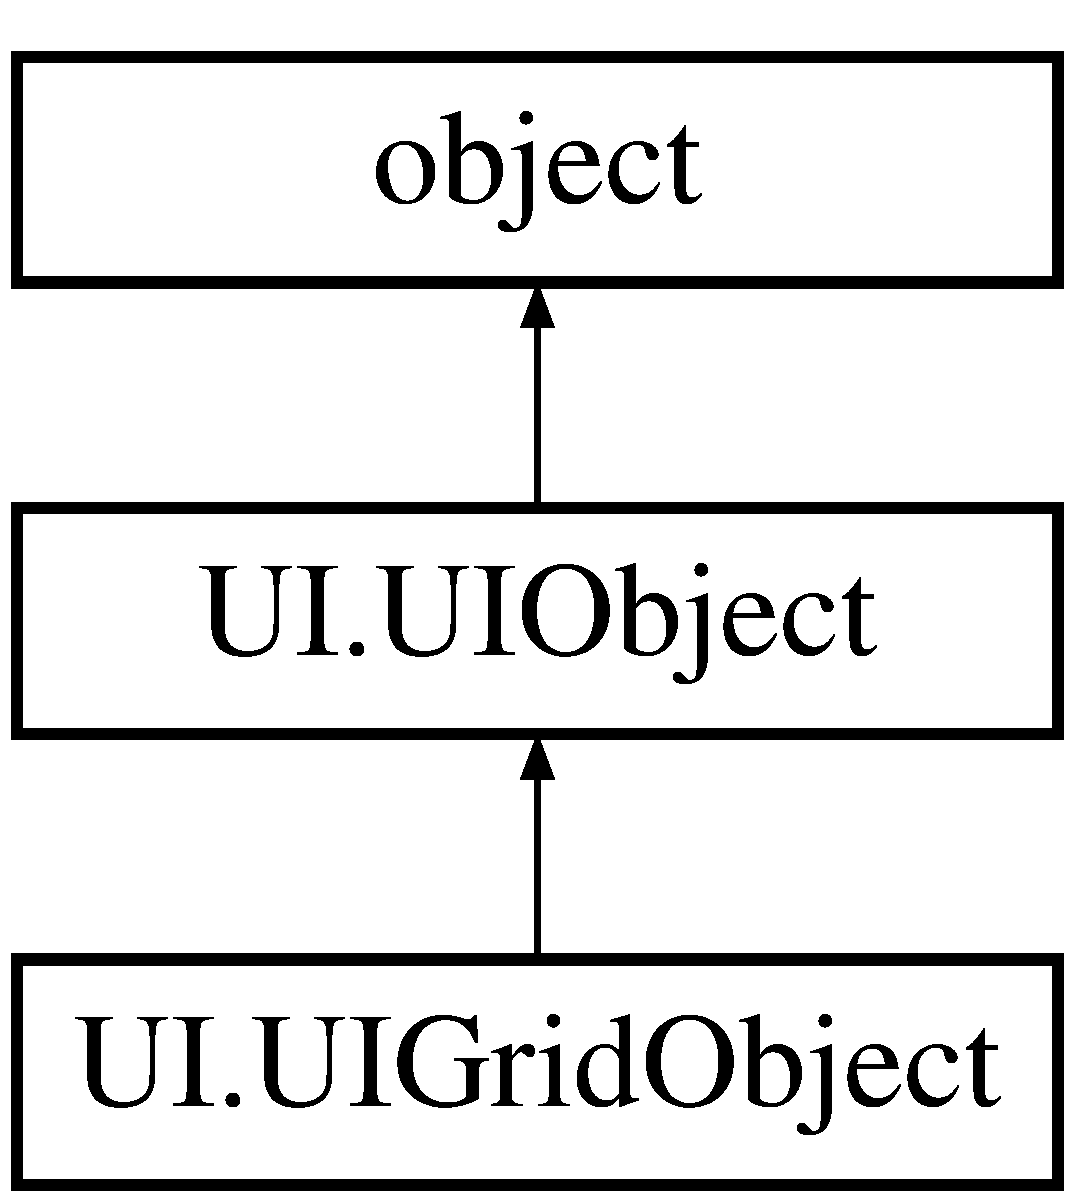
\includegraphics[height=3.000000cm]{classUI_1_1UIGridObject}
\end{center}
\end{figure}
\subsection*{Public Member Functions}
\begin{DoxyCompactItemize}
\item 
\hypertarget{classUI_1_1UIGridObject_acbf499a6157cb0cde43081bbff3074cd}{def {\bfseries \-\_\-\-\_\-init\-\_\-\-\_\-}}\label{classUI_1_1UIGridObject_acbf499a6157cb0cde43081bbff3074cd}

\end{DoxyCompactItemize}
\subsection*{Data Fields}
\begin{DoxyCompactItemize}
\item 
\hypertarget{classUI_1_1UIGridObject_a4029d3dcf3e99bb3421e00848f72028b}{{\bfseries grid}}\label{classUI_1_1UIGridObject_a4029d3dcf3e99bb3421e00848f72028b}

\item 
\hypertarget{classUI_1_1UIGridObject_a4fd5fc4e243ab419ea28b6321cb24f19}{{\bfseries rel\-\_\-x}}\label{classUI_1_1UIGridObject_a4fd5fc4e243ab419ea28b6321cb24f19}

\item 
\hypertarget{classUI_1_1UIGridObject_ad1e46510929ad0f70911329409494e51}{{\bfseries rel\-\_\-y}}\label{classUI_1_1UIGridObject_ad1e46510929ad0f70911329409494e51}

\end{DoxyCompactItemize}
\subsection*{Properties}
\begin{DoxyCompactItemize}
\item 
\hypertarget{classUI_1_1UIGridObject_a1f2a8d84439799685b761a30c5816ac1}{{\bfseries grid\-\_\-x} = property(\-\_\-get\-\_\-grid\-\_\-x, \-\_\-set\-\_\-grid\-\_\-x)}\label{classUI_1_1UIGridObject_a1f2a8d84439799685b761a30c5816ac1}

\item 
\hypertarget{classUI_1_1UIGridObject_a2aad24251d1eda51b9ad202998c435c7}{{\bfseries grid\-\_\-y} = property(\-\_\-get\-\_\-grid\-\_\-y, \-\_\-set\-\_\-grid\-\_\-y)}\label{classUI_1_1UIGridObject_a2aad24251d1eda51b9ad202998c435c7}

\item 
\hypertarget{classUI_1_1UIGridObject_aa17c84259775d825baaf5c504f6d14f3}{{\bfseries grid\-\_\-pos} = property(\-\_\-get\-\_\-grid\-\_\-pos, \-\_\-set\-\_\-grid\-\_\-pos)}\label{classUI_1_1UIGridObject_aa17c84259775d825baaf5c504f6d14f3}

\end{DoxyCompactItemize}


\subsection{Detailed Description}
\begin{DoxyVerb}Base class of everything that's on a grid.

Instances have the following attributes:
- pos      = x, y           = position on screen
- rel_pos  = rel_x, rel_y   = position relative to parent
- grid_pos = grid_x, grid_y = position on grid
- size     = width, height  = size
\end{DoxyVerb}
 

Definition at line 62 of file U\-I.\-py.



The documentation for this class was generated from the following file\-:\begin{DoxyCompactItemize}
\item 
/home/antipant/\-Protocol\-P\-\_\-\-Project/\-U\-I/U\-I.\-py\end{DoxyCompactItemize}

\hypertarget{classUI_1_1UIObject}{\section{U\-I.\-U\-I\-Object Class Reference}
\label{classUI_1_1UIObject}\index{U\-I.\-U\-I\-Object@{U\-I.\-U\-I\-Object}}
}
Inheritance diagram for U\-I.\-U\-I\-Object\-:\begin{figure}[H]
\begin{center}
\leavevmode
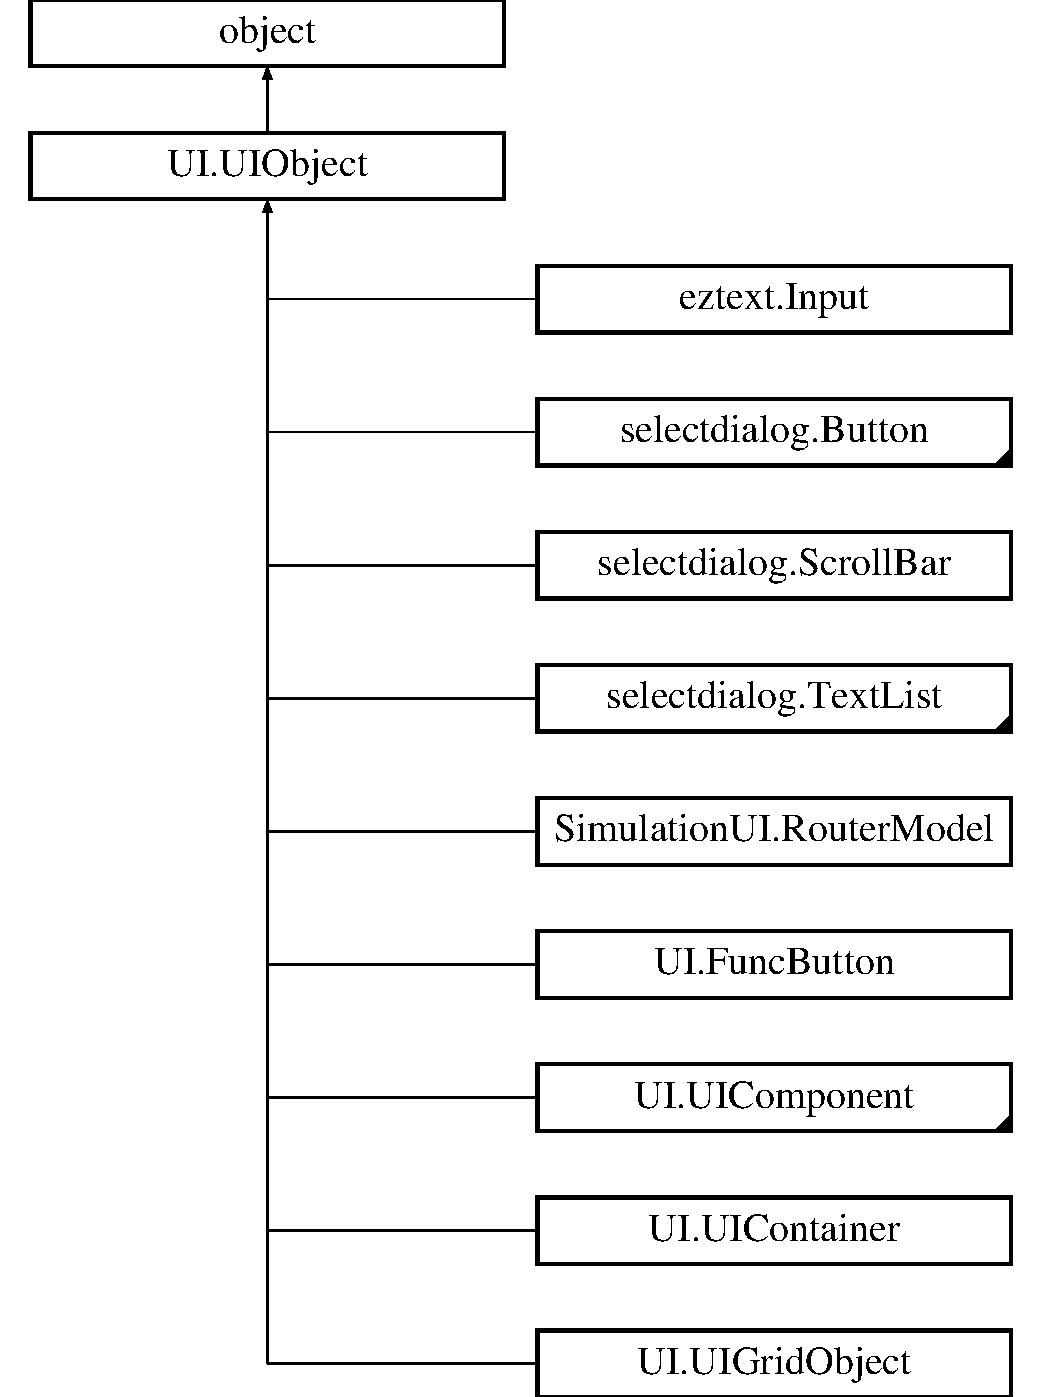
\includegraphics[height=11.000000cm]{classUI_1_1UIObject}
\end{center}
\end{figure}
\subsection*{Public Member Functions}
\begin{DoxyCompactItemize}
\item 
\hypertarget{classUI_1_1UIObject_a24d9ef66ab90afb40f24e2f1accd749a}{def {\bfseries \-\_\-\-\_\-init\-\_\-\-\_\-}}\label{classUI_1_1UIObject_a24d9ef66ab90afb40f24e2f1accd749a}

\item 
\hypertarget{classUI_1_1UIObject_aa4c5ce87542d83316f80a96520a93be0}{def {\bfseries contains}}\label{classUI_1_1UIObject_aa4c5ce87542d83316f80a96520a93be0}

\item 
\hypertarget{classUI_1_1UIObject_a87ca04ede1213b54c928aa6228180583}{def {\bfseries translate}}\label{classUI_1_1UIObject_a87ca04ede1213b54c928aa6228180583}

\end{DoxyCompactItemize}
\subsection*{Data Fields}
\begin{DoxyCompactItemize}
\item 
\hypertarget{classUI_1_1UIObject_a0ca2ea83453a41066c5e606952266e9a}{{\bfseries parent}}\label{classUI_1_1UIObject_a0ca2ea83453a41066c5e606952266e9a}

\item 
\hypertarget{classUI_1_1UIObject_a0a9fe60c4e321830baa54329192f0931}{{\bfseries x}}\label{classUI_1_1UIObject_a0a9fe60c4e321830baa54329192f0931}

\item 
\hypertarget{classUI_1_1UIObject_a7e9a5c2f43265a757d4c90089e58a8e5}{{\bfseries y}}\label{classUI_1_1UIObject_a7e9a5c2f43265a757d4c90089e58a8e5}

\end{DoxyCompactItemize}
\subsection*{Properties}
\begin{DoxyCompactItemize}
\item 
\hypertarget{classUI_1_1UIObject_ad1f2cc2a5531c13ff9a7627b2218a1a0}{{\bfseries pos} = property(\-\_\-get\-\_\-pos, \-\_\-set\-\_\-pos)}\label{classUI_1_1UIObject_ad1f2cc2a5531c13ff9a7627b2218a1a0}

\item 
\hypertarget{classUI_1_1UIObject_a9558ebeab6d04876a9ad0ac629622452}{{\bfseries rel\-\_\-x} = property(\-\_\-get\-\_\-rel\-\_\-x, \-\_\-set\-\_\-rel\-\_\-x)}\label{classUI_1_1UIObject_a9558ebeab6d04876a9ad0ac629622452}

\item 
\hypertarget{classUI_1_1UIObject_ac5225d93c0951e718a9e966bc1ada531}{{\bfseries rel\-\_\-y} = property(\-\_\-get\-\_\-rel\-\_\-y, \-\_\-set\-\_\-rel\-\_\-y)}\label{classUI_1_1UIObject_ac5225d93c0951e718a9e966bc1ada531}

\item 
\hypertarget{classUI_1_1UIObject_a2b7d8794830d49093f05e017ca23768f}{{\bfseries rel\-\_\-pos} = property(\-\_\-get\-\_\-rel\-\_\-pos, \-\_\-set\-\_\-rel\-\_\-pos)}\label{classUI_1_1UIObject_a2b7d8794830d49093f05e017ca23768f}

\item 
\hypertarget{classUI_1_1UIObject_aa51a72c7559fed4f260b192a12e6805c}{{\bfseries size} = property(\-\_\-get\-\_\-size, \-\_\-set\-\_\-size)}\label{classUI_1_1UIObject_aa51a72c7559fed4f260b192a12e6805c}

\item 
\hypertarget{classUI_1_1UIObject_a72e5ff37f9a27451cc7a586fa43fdb9c}{{\bfseries rect} = property(\-\_\-get\-\_\-rect)}\label{classUI_1_1UIObject_a72e5ff37f9a27451cc7a586fa43fdb9c}

\end{DoxyCompactItemize}


\subsection{Detailed Description}
\begin{DoxyVerb}Base class of everything with coordinates.

Instances have the following attributes:
- pos     = x, y          = position on screen
- rel_pos = rel_x, rel_y  = position relative to parent
- size    = width, height = size
\end{DoxyVerb}
 

Definition at line 17 of file U\-I.\-py.



The documentation for this class was generated from the following file\-:\begin{DoxyCompactItemize}
\item 
/home/antipant/\-Protocol\-P\-\_\-\-Project/\-U\-I/U\-I.\-py\end{DoxyCompactItemize}

\hypertarget{classUI_1_1UIRoot}{\section{U\-I.\-U\-I\-Root Class Reference}
\label{classUI_1_1UIRoot}\index{U\-I.\-U\-I\-Root@{U\-I.\-U\-I\-Root}}
}
\subsection*{Public Member Functions}
\begin{DoxyCompactItemize}
\item 
\hypertarget{classUI_1_1UIRoot_a4265dd3ffbe5fe9fd1847e3ce0b000f8}{def {\bfseries \-\_\-\-\_\-init\-\_\-\-\_\-}}\label{classUI_1_1UIRoot_a4265dd3ffbe5fe9fd1847e3ce0b000f8}

\end{DoxyCompactItemize}
\subsection*{Data Fields}
\begin{DoxyCompactItemize}
\item 
\hypertarget{classUI_1_1UIRoot_a5674fee74d86fd3c98a87b820dc8f714}{{\bfseries x}}\label{classUI_1_1UIRoot_a5674fee74d86fd3c98a87b820dc8f714}

\item 
\hypertarget{classUI_1_1UIRoot_a19c3889a07c37e6330eca943e31c6e19}{{\bfseries y}}\label{classUI_1_1UIRoot_a19c3889a07c37e6330eca943e31c6e19}

\end{DoxyCompactItemize}


\subsection{Detailed Description}


Definition at line 13 of file U\-I.\-py.



The documentation for this class was generated from the following file\-:\begin{DoxyCompactItemize}
\item 
/home/antipant/\-Protocol\-P\-\_\-\-Project/\-U\-I/U\-I.\-py\end{DoxyCompactItemize}

\hypertarget{classselectdialog_1_1Window}{\section{selectdialog.\-Window Class Reference}
\label{classselectdialog_1_1Window}\index{selectdialog.\-Window@{selectdialog.\-Window}}
}
\subsection*{Public Member Functions}
\begin{DoxyCompactItemize}
\item 
\hypertarget{classselectdialog_1_1Window_a4aed47eb64a7fda5d4350375702f0a94}{def {\bfseries \-\_\-\-\_\-init\-\_\-\-\_\-}}\label{classselectdialog_1_1Window_a4aed47eb64a7fda5d4350375702f0a94}

\item 
\hypertarget{classselectdialog_1_1Window_a58114bdf1bcb10b3545775bef7898718}{def {\bfseries draw}}\label{classselectdialog_1_1Window_a58114bdf1bcb10b3545775bef7898718}

\item 
\hypertarget{classselectdialog_1_1Window_acb02a8142ed86ebb264b8a9f917c9aff}{def {\bfseries loop}}\label{classselectdialog_1_1Window_acb02a8142ed86ebb264b8a9f917c9aff}

\end{DoxyCompactItemize}
\subsection*{Data Fields}
\begin{DoxyCompactItemize}
\item 
\hypertarget{classselectdialog_1_1Window_a4d154a9aad52ec0692243f5d7739be89}{{\bfseries screen}}\label{classselectdialog_1_1Window_a4d154a9aad52ec0692243f5d7739be89}

\item 
\hypertarget{classselectdialog_1_1Window_a951affeeac2b26a695a1dfcf84f314d2}{{\bfseries background}}\label{classselectdialog_1_1Window_a951affeeac2b26a695a1dfcf84f314d2}

\item 
\hypertarget{classselectdialog_1_1Window_a6d451cac38094e53e6689926b68c103d}{{\bfseries fps}}\label{classselectdialog_1_1Window_a6d451cac38094e53e6689926b68c103d}

\item 
\hypertarget{classselectdialog_1_1Window_a0570579a24621ecd5379ca938fa93b7e}{{\bfseries clock}}\label{classselectdialog_1_1Window_a0570579a24621ecd5379ca938fa93b7e}

\item 
\hypertarget{classselectdialog_1_1Window_a23eaef8cb0578292c0688a75a2618ebd}{{\bfseries res}}\label{classselectdialog_1_1Window_a23eaef8cb0578292c0688a75a2618ebd}

\item 
\hypertarget{classselectdialog_1_1Window_ac36daf62be1aff528d4833b9403d707f}{{\bfseries elems}}\label{classselectdialog_1_1Window_ac36daf62be1aff528d4833b9403d707f}

\item 
\hypertarget{classselectdialog_1_1Window_a1fd14a231e97c762f526771e35b75e05}{{\bfseries sprites}}\label{classselectdialog_1_1Window_a1fd14a231e97c762f526771e35b75e05}

\item 
\hypertarget{classselectdialog_1_1Window_a4ea42ee5e2971e051fea5c432df4d2f8}{{\bfseries done}}\label{classselectdialog_1_1Window_a4ea42ee5e2971e051fea5c432df4d2f8}

\end{DoxyCompactItemize}


\subsection{Detailed Description}


Definition at line 21 of file selectdialog.\-py.



The documentation for this class was generated from the following file\-:\begin{DoxyCompactItemize}
\item 
/home/antipant/\-Protocol\-P\-\_\-\-Project/\-U\-I/selectdialog.\-py\end{DoxyCompactItemize}

\chapter{File Documentation}
\hypertarget{BGPMessage_8cpp}{\section{/home/antipant/\-Protocol\-P\-\_\-\-Project/\-B\-G\-P\-Message.cpp File Reference}
\label{BGPMessage_8cpp}\index{/home/antipant/\-Protocol\-P\-\_\-\-Project/\-B\-G\-P\-Message.\-cpp@{/home/antipant/\-Protocol\-P\-\_\-\-Project/\-B\-G\-P\-Message.\-cpp}}
}


Implementation of \hyperlink{classBGPMessage}{B\-G\-P\-Message} class.  


{\ttfamily \#include \char`\"{}B\-G\-P\-Message.\-hpp\char`\"{}}\\*


\subsection{Detailed Description}
Implementation of \hyperlink{classBGPMessage}{B\-G\-P\-Message} class. \begin{DoxyAuthor}{Author}
Antti Siirilä, 501449 
\end{DoxyAuthor}
\begin{DoxyVersion}{Version}
1.\-0 
\end{DoxyVersion}
\begin{DoxyDate}{Date}
11.\-2.\-2013 
\end{DoxyDate}


Definition in file \hyperlink{BGPMessage_8cpp_source}{B\-G\-P\-Message.\-cpp}.


\hypertarget{BGPMessage_8hpp}{\section{/home/antipant/\-Protocol\-P\-\_\-\-Project/\-B\-G\-P\-Message.hpp File Reference}
\label{BGPMessage_8hpp}\index{/home/antipant/\-Protocol\-P\-\_\-\-Project/\-B\-G\-P\-Message.\-hpp@{/home/antipant/\-Protocol\-P\-\_\-\-Project/\-B\-G\-P\-Message.\-hpp}}
}


Header file of B\-G\-P message class.  


{\ttfamily \#include $<$systemc$>$}\\*
\subsection*{Data Structures}
\begin{DoxyCompactItemize}
\item 
class \hyperlink{classBGPMessage}{B\-G\-P\-Message}
\end{DoxyCompactItemize}
\subsection*{Macros}
\begin{DoxyCompactItemize}
\item 
\#define \hyperlink{BGPMessage_8hpp_a1354b70ac6803a06beebe84f61b5f95b}{O\-P\-E\-N}~1
\begin{DoxyCompactList}\small\item\em B\-G\-P message type definitions. \end{DoxyCompactList}\item 
\hypertarget{BGPMessage_8hpp_ac2558c32fa879d85fe59f8c5f8dfbc04}{\#define \hyperlink{BGPMessage_8hpp_ac2558c32fa879d85fe59f8c5f8dfbc04}{U\-P\-D\-A\-T\-E}~2}\label{BGPMessage_8hpp_ac2558c32fa879d85fe59f8c5f8dfbc04}

\begin{DoxyCompactList}\small\item\em Defines the B\-G\-P update message type value. \end{DoxyCompactList}\item 
\hypertarget{BGPMessage_8hpp_a6985e58a0ff3195dca91e5aaca02e372}{\#define \hyperlink{BGPMessage_8hpp_a6985e58a0ff3195dca91e5aaca02e372}{N\-O\-T\-I\-F\-I\-C\-A\-T\-I\-O\-N}~3}\label{BGPMessage_8hpp_a6985e58a0ff3195dca91e5aaca02e372}

\begin{DoxyCompactList}\small\item\em Defines the B\-G\-P notification message type value. \end{DoxyCompactList}\item 
\hypertarget{BGPMessage_8hpp_ab42bd8b11f355b81223ae2974c9634f5}{\#define \hyperlink{BGPMessage_8hpp_ab42bd8b11f355b81223ae2974c9634f5}{K\-E\-E\-P\-A\-L\-I\-V\-E}~4}\label{BGPMessage_8hpp_ab42bd8b11f355b81223ae2974c9634f5}

\begin{DoxyCompactList}\small\item\em Defines the B\-G\-P keepalive message type value. \end{DoxyCompactList}\item 
\hypertarget{BGPMessage_8hpp_a6020613f5062417d9811cfa837215c83}{\#define \hyperlink{BGPMessage_8hpp_a6020613f5062417d9811cfa837215c83}{T\-C\-P\-\_\-\-S\-Y\-N}~5}\label{BGPMessage_8hpp_a6020613f5062417d9811cfa837215c83}

\begin{DoxyCompactList}\small\item\em Defines the T\-C\-P syn message type. \end{DoxyCompactList}\item 
\hypertarget{BGPMessage_8hpp_a6df99e63a8c6c13ba0809acbe893bf0a}{\#define \hyperlink{BGPMessage_8hpp_a6df99e63a8c6c13ba0809acbe893bf0a}{T\-C\-P\-\_\-\-S\-Y\-N\-A\-C\-K}~6}\label{BGPMessage_8hpp_a6df99e63a8c6c13ba0809acbe893bf0a}

\begin{DoxyCompactList}\small\item\em Defines the T\-C\-P synack message type. \end{DoxyCompactList}\item 
\hypertarget{BGPMessage_8hpp_a44b3b1ab31a403ba28ec135adfcbefef}{\#define \hyperlink{BGPMessage_8hpp_a44b3b1ab31a403ba28ec135adfcbefef}{T\-C\-P\-\_\-\-A\-C\-K}~7}\label{BGPMessage_8hpp_a44b3b1ab31a403ba28ec135adfcbefef}

\begin{DoxyCompactList}\small\item\em Defines the T\-C\-P ack message type. \end{DoxyCompactList}\end{DoxyCompactItemize}


\subsection{Detailed Description}
Header file of B\-G\-P message class. defines the \hyperlink{classBGPMessage}{B\-G\-P\-Message} class. \begin{DoxyAuthor}{Author}
Antti Siirilä, 501449 
\end{DoxyAuthor}
\begin{DoxyVersion}{Version}
1.\-0 
\end{DoxyVersion}
\begin{DoxyDate}{Date}
11.\-2.\-2013 
\end{DoxyDate}


Definition in file \hyperlink{BGPMessage_8hpp_source}{B\-G\-P\-Message.\-hpp}.



\subsection{Macro Definition Documentation}
\hypertarget{BGPMessage_8hpp_a1354b70ac6803a06beebe84f61b5f95b}{\index{B\-G\-P\-Message.\-hpp@{B\-G\-P\-Message.\-hpp}!O\-P\-E\-N@{O\-P\-E\-N}}
\index{O\-P\-E\-N@{O\-P\-E\-N}!BGPMessage.hpp@{B\-G\-P\-Message.\-hpp}}
\subsubsection[{O\-P\-E\-N}]{\setlength{\rightskip}{0pt plus 5cm}\#define O\-P\-E\-N~1}}\label{BGPMessage_8hpp_a1354b70ac6803a06beebe84f61b5f95b}


B\-G\-P message type definitions. 

1 -\/ O\-P\-E\-N, 2 -\/ U\-P\-D\-A\-T\-E, 3 -\/ N\-O\-T\-I\-F\-I\-C\-A\-T\-I\-O\-N, 4 -\/ K\-E\-E\-P\-A\-L\-I\-V\-E

Defines the B\-G\-P open message type value 

Definition at line 39 of file B\-G\-P\-Message.\-hpp.


\hypertarget{BGPSession_8cpp}{\section{/home/antipant/\-Protocol\-P\-\_\-\-Project/\-B\-G\-P\-Session.cpp File Reference}
\label{BGPSession_8cpp}\index{/home/antipant/\-Protocol\-P\-\_\-\-Project/\-B\-G\-P\-Session.\-cpp@{/home/antipant/\-Protocol\-P\-\_\-\-Project/\-B\-G\-P\-Session.\-cpp}}
}


Implementation of \hyperlink{classBGPSession}{B\-G\-P\-Session}.  


{\ttfamily \#include \char`\"{}B\-G\-P\-Session.\-hpp\char`\"{}}\\*
{\ttfamily \#include \char`\"{}Report\-Globals.\-hpp\char`\"{}}\\*


\subsection{Detailed Description}
Implementation of \hyperlink{classBGPSession}{B\-G\-P\-Session}. \begin{DoxyAuthor}{Author}
Antti Siirilä, 501449 
\end{DoxyAuthor}
\begin{DoxyVersion}{Version}
1.\-0 
\end{DoxyVersion}
\begin{DoxyDate}{Date}
Wed Feb 13 20\-:36\-:28 2013 
\end{DoxyDate}


Definition in file \hyperlink{BGPSession_8cpp_source}{B\-G\-P\-Session.\-cpp}.


\hypertarget{BGPSession_8hpp}{\section{/home/antipant/\-Protocol\-P\-\_\-\-Project/\-B\-G\-P\-Session.hpp File Reference}
\label{BGPSession_8hpp}\index{/home/antipant/\-Protocol\-P\-\_\-\-Project/\-B\-G\-P\-Session.\-hpp@{/home/antipant/\-Protocol\-P\-\_\-\-Project/\-B\-G\-P\-Session.\-hpp}}
}


Header file of \hyperlink{classBGPSession}{B\-G\-P\-Session} module.  


{\ttfamily \#include \char`\"{}systemc\char`\"{}}\\*
{\ttfamily \#include \char`\"{}B\-G\-P\-Session\-\_\-\-If.\-hpp\char`\"{}}\\*
{\ttfamily \#include \char`\"{}B\-G\-P\-Message.\-hpp\char`\"{}}\\*
{\ttfamily \#include \char`\"{}Configuration.\-hpp\char`\"{}}\\*
{\ttfamily \#include \char`\"{}Output\-\_\-\-If.\-hpp\char`\"{}}\\*
{\ttfamily \#include \char`\"{}String\-Tools.\-hpp\char`\"{}}\\*
{\ttfamily \#include \char`\"{}Interface\-\_\-\-If.\-hpp\char`\"{}}\\*
\subsection*{Data Structures}
\begin{DoxyCompactItemize}
\item 
class \hyperlink{classBGPSession}{B\-G\-P\-Session}
\begin{DoxyCompactList}\small\item\em \hyperlink{classBGPSession}{B\-G\-P\-Session} module handles the Hold\-Down and Keepalive timers of the session and sends keepalive messages to the session peer. \end{DoxyCompactList}\end{DoxyCompactItemize}
\subsection*{Macros}
\begin{DoxyCompactItemize}
\item 
\hypertarget{BGPSession_8hpp_a5ae6f07aa75aad273ae0dc9c2580e9e5}{\#define {\bfseries T\-C\-P\-\_\-\-R\-T\-\_\-\-D\-E\-L\-A\-Y}~20}\label{BGPSession_8hpp_a5ae6f07aa75aad273ae0dc9c2580e9e5}

\item 
\hypertarget{BGPSession_8hpp_a9bd1caf41aa7de01fc1fdd395dd1df9c}{\#define {\bfseries O\-P\-E\-N\-S\-E\-N\-D\-\_\-\-R\-T\-\_\-\-D\-E\-L\-A\-Y}~20}\label{BGPSession_8hpp_a9bd1caf41aa7de01fc1fdd395dd1df9c}

\end{DoxyCompactItemize}
\subsection*{Enumerations}
\begin{DoxyCompactItemize}
\item 
enum {\bfseries B\-G\-P\-\_\-\-States} \{ \\*
{\bfseries I\-D\-L\-E}, 
{\bfseries C\-O\-N\-N\-E\-C\-T}, 
{\bfseries A\-C\-T\-I\-V\-E}, 
{\bfseries O\-P\-E\-N\-\_\-\-S\-E\-N\-T}, 
\\*
{\bfseries O\-P\-E\-N\-\_\-\-C\-O\-N\-F\-I\-R\-M}, 
{\bfseries E\-S\-T\-A\-B\-L\-I\-S\-H\-E\-D}
 \}
\item 
enum {\bfseries T\-C\-P\-\_\-\-States} \{ {\bfseries S\-Y\-N}, 
{\bfseries A\-C\-K}, 
{\bfseries O\-P\-E\-N\-\_\-\-S\-E\-N\-D}
 \}
\end{DoxyCompactItemize}


\subsection{Detailed Description}
Header file of \hyperlink{classBGPSession}{B\-G\-P\-Session} module. \begin{DoxyAuthor}{Author}
Antti Siirilä, 501449 
\end{DoxyAuthor}
\begin{DoxyVersion}{Version}
1.\-0 
\end{DoxyVersion}
\begin{DoxyDate}{Date}
12.\-2.\-2013 
\end{DoxyDate}


Definition in file \hyperlink{BGPSession_8hpp_source}{B\-G\-P\-Session.\-hpp}.


\hypertarget{BGPSession__If_8hpp}{\section{/home/antipant/\-Protocol\-P\-\_\-\-Project/\-B\-G\-P\-Session\-\_\-\-If.hpp File Reference}
\label{BGPSession__If_8hpp}\index{/home/antipant/\-Protocol\-P\-\_\-\-Project/\-B\-G\-P\-Session\-\_\-\-If.\-hpp@{/home/antipant/\-Protocol\-P\-\_\-\-Project/\-B\-G\-P\-Session\-\_\-\-If.\-hpp}}
}
{\ttfamily \#include \char`\"{}systemc\char`\"{}}\\*
\subsection*{Data Structures}
\begin{DoxyCompactItemize}
\item 
class \hyperlink{classBGPSession__If}{B\-G\-P\-Session\-\_\-\-If}
\end{DoxyCompactItemize}


\subsection{Detailed Description}
\begin{DoxyAuthor}{Author}
Antti Siirilä, 501449 
\end{DoxyAuthor}
\begin{DoxyVersion}{Version}
1.\-0 
\end{DoxyVersion}
\begin{DoxyDate}{Date}
Tue Feb 12 13\-:01\-:27 2013 
\end{DoxyDate}


Definition in file \hyperlink{BGPSession__If_8hpp_source}{B\-G\-P\-Session\-\_\-\-If.\-hpp}.


\hypertarget{Communication__If_8hpp}{\section{/home/antipant/\-Protocol\-P\-\_\-\-Project/\-Communication\-\_\-\-If.hpp File Reference}
\label{Communication__If_8hpp}\index{/home/antipant/\-Protocol\-P\-\_\-\-Project/\-Communication\-\_\-\-If.\-hpp@{/home/antipant/\-Protocol\-P\-\_\-\-Project/\-Communication\-\_\-\-If.\-hpp}}
}
{\ttfamily \#include \char`\"{}systemc\char`\"{}}\\*
{\ttfamily \#include \char`\"{}Packet.\-hpp\char`\"{}}\\*
\subsection*{Data Structures}
\begin{DoxyCompactItemize}
\item 
class \hyperlink{classCommunication__If}{Communication\-\_\-\-If}
\end{DoxyCompactItemize}


\subsection{Detailed Description}
\begin{DoxyAuthor}{Author}
Antti Siirilä, 501449 
\end{DoxyAuthor}
\begin{DoxyVersion}{Version}
1.\-0 
\end{DoxyVersion}
\begin{DoxyDate}{Date}
03.\-05.\-2013 
\end{DoxyDate}


Definition in file \hyperlink{Communication__If_8hpp_source}{Communication\-\_\-\-If.\-hpp}.


\input{Configuration_8cpp}
\hypertarget{Configuration_8hpp}{\section{/home/antipant/\-Protocol\-P\-\_\-\-Project/\-Configuration.hpp File Reference}
\label{Configuration_8hpp}\index{/home/antipant/\-Protocol\-P\-\_\-\-Project/\-Configuration.\-hpp@{/home/antipant/\-Protocol\-P\-\_\-\-Project/\-Configuration.\-hpp}}
}


Defines the \hyperlink{classBGPSessionParameters}{B\-G\-P\-Session\-Parameters},\hyperlink{classControlPlaneConfig}{Control\-Plane\-Config}, \hyperlink{classConnection}{Connection}, \hyperlink{classRouterConfig}{Router\-Config}, and \hyperlink{classSimulationConfig}{Simulation\-Config} classes.  


{\ttfamily \#include \char`\"{}systemc\char`\"{}}\\*
{\ttfamily \#include \char`\"{}String\-Tools.\-hpp\char`\"{}}\\*
\subsection*{Data Structures}
\begin{DoxyCompactItemize}
\item 
class \hyperlink{classBGPSessionParameters}{B\-G\-P\-Session\-Parameters}
\begin{DoxyCompactList}\small\item\em Holds the parameters for B\-G\-P session. \end{DoxyCompactList}\item 
class \hyperlink{classControlPlaneConfig}{Control\-Plane\-Config}
\begin{DoxyCompactList}\small\item\em Holds the B\-G\-P parameters. \end{DoxyCompactList}\item 
class \hyperlink{classConnection}{Connection}
\begin{DoxyCompactList}\small\item\em Holds the connection parameters for local interface. \end{DoxyCompactList}\item 
class \hyperlink{classRouterConfig}{Router\-Config}
\begin{DoxyCompactList}\small\item\em Holds the parameters for a router including interface connection parameters. \end{DoxyCompactList}\item 
class \hyperlink{classSimulationConfig}{Simulation\-Config}
\begin{DoxyCompactList}\small\item\em Holds all the simulation parameters received from G\-U\-I. \end{DoxyCompactList}\end{DoxyCompactItemize}
\subsection*{Macros}
\begin{DoxyCompactItemize}
\item 
\hypertarget{Configuration_8hpp_af19f26460d89cfb3f212f4b0a44882e8}{\#define {\bfseries C\-L\-I\-E\-N\-T}~1}\label{Configuration_8hpp_af19f26460d89cfb3f212f4b0a44882e8}

\item 
\hypertarget{Configuration_8hpp_a24cd3c37a165a8c4626d9e78df4574ff}{\#define {\bfseries S\-E\-R\-V\-E\-R}~0}\label{Configuration_8hpp_a24cd3c37a165a8c4626d9e78df4574ff}

\end{DoxyCompactItemize}


\subsection{Detailed Description}
Defines the \hyperlink{classBGPSessionParameters}{B\-G\-P\-Session\-Parameters},\hyperlink{classControlPlaneConfig}{Control\-Plane\-Config}, \hyperlink{classConnection}{Connection}, \hyperlink{classRouterConfig}{Router\-Config}, and \hyperlink{classSimulationConfig}{Simulation\-Config} classes. \begin{DoxyAuthor}{Author}
Antti Siirilä, 501449 
\end{DoxyAuthor}
\begin{DoxyVersion}{Version}
1.\-0 
\end{DoxyVersion}
\begin{DoxyDate}{Date}
Wed Mar 20 15\-:30\-:11 2013 
\end{DoxyDate}


Definition in file \hyperlink{Configuration_8hpp_source}{Configuration.\-hpp}.


\hypertarget{ControlPlane_8cpp}{\section{/home/antipant/\-Protocol\-P\-\_\-\-Project/\-Control\-Plane.cpp File Reference}
\label{ControlPlane_8cpp}\index{/home/antipant/\-Protocol\-P\-\_\-\-Project/\-Control\-Plane.\-cpp@{/home/antipant/\-Protocol\-P\-\_\-\-Project/\-Control\-Plane.\-cpp}}
}


Implementation of \hyperlink{classControlPlane}{Control\-Plane}.  


{\ttfamily \#include \char`\"{}Control\-Plane.\-hpp\char`\"{}}\\*
{\ttfamily \#include \char`\"{}Report\-Globals.\-hpp\char`\"{}}\\*


\subsection{Detailed Description}
Implementation of \hyperlink{classControlPlane}{Control\-Plane}. \begin{DoxyAuthor}{Author}
Antti Siiril�, 501449 
\end{DoxyAuthor}
\begin{DoxyVersion}{Version}
1.\-0 
\end{DoxyVersion}
\begin{DoxyDate}{Date}
Tue Feb 12 12\-:32\-:09 2013 
\end{DoxyDate}


Definition in file \hyperlink{ControlPlane_8cpp_source}{Control\-Plane.\-cpp}.


\hypertarget{ControlPlane_8hpp}{\section{/home/antipant/\-Protocol\-P\-\_\-\-Project/\-Control\-Plane.hpp File Reference}
\label{ControlPlane_8hpp}\index{/home/antipant/\-Protocol\-P\-\_\-\-Project/\-Control\-Plane.\-hpp@{/home/antipant/\-Protocol\-P\-\_\-\-Project/\-Control\-Plane.\-hpp}}
}


Header file of \hyperlink{classControlPlane}{Control\-Plane} module.  


{\ttfamily \#include \char`\"{}systemc\char`\"{}}\\*
{\ttfamily \#include \char`\"{}B\-G\-P\-Message.\-hpp\char`\"{}}\\*
{\ttfamily \#include \char`\"{}Configuration.\-hpp\char`\"{}}\\*
{\ttfamily \#include \char`\"{}B\-G\-P\-Session.\-hpp\char`\"{}}\\*
{\ttfamily \#include \char`\"{}B\-G\-P\-Session\-\_\-\-If.\-hpp\char`\"{}}\\*
{\ttfamily \#include \char`\"{}Routing\-Table\-\_\-\-If.\-hpp\char`\"{}}\\*
{\ttfamily \#include \char`\"{}String\-Tools.\-hpp\char`\"{}}\\*
{\ttfamily \#include \char`\"{}Output\-\_\-\-If.\-hpp\char`\"{}}\\*
{\ttfamily \#include \char`\"{}Interface\-\_\-\-If.\-hpp\char`\"{}}\\*
\subsection*{Data Structures}
\begin{DoxyCompactItemize}
\item 
class \hyperlink{classControlPlane}{Control\-Plane}
\begin{DoxyCompactList}\small\item\em \hyperlink{classControlPlane}{Control\-Plane} module runs the B\-G\-P process. \end{DoxyCompactList}\end{DoxyCompactItemize}


\subsection{Detailed Description}
Header file of \hyperlink{classControlPlane}{Control\-Plane} module. \begin{DoxyAuthor}{Author}
Antti Siirilä, 501449 
\end{DoxyAuthor}
\begin{DoxyVersion}{Version}
1.\-0 
\end{DoxyVersion}
\begin{DoxyDate}{Date}
12.\-2.\-2013 
\end{DoxyDate}


Definition in file \hyperlink{ControlPlane_8hpp_source}{Control\-Plane.\-hpp}.


\hypertarget{DataPlane_8cpp}{\section{/home/antipant/\-Protocol\-P\-\_\-\-Project/\-Data\-Plane.cpp File Reference}
\label{DataPlane_8cpp}\index{/home/antipant/\-Protocol\-P\-\_\-\-Project/\-Data\-Plane.\-cpp@{/home/antipant/\-Protocol\-P\-\_\-\-Project/\-Data\-Plane.\-cpp}}
}
{\ttfamily \#include \char`\"{}Data\-Plane.\-hpp\char`\"{}}\\*
{\ttfamily \#include \char`\"{}Report\-Globals.\-hpp\char`\"{}}\\*


\subsection{Detailed Description}
\begin{DoxyAuthor}{Author}
Antti Siirilä, 501449 
\end{DoxyAuthor}
\begin{DoxyVersion}{Version}
1.\-0 
\end{DoxyVersion}
\begin{DoxyDate}{Date}
Tue Feb 12 12\-:14\-:35 2013 
\end{DoxyDate}


Definition in file \hyperlink{DataPlane_8cpp_source}{Data\-Plane.\-cpp}.


\hypertarget{DataPlane_8hpp}{\section{/home/antipant/\-Protocol\-P\-\_\-\-Project/\-Data\-Plane.hpp File Reference}
\label{DataPlane_8hpp}\index{/home/antipant/\-Protocol\-P\-\_\-\-Project/\-Data\-Plane.\-hpp@{/home/antipant/\-Protocol\-P\-\_\-\-Project/\-Data\-Plane.\-hpp}}
}
{\ttfamily \#include \char`\"{}systemc\char`\"{}}\\*
{\ttfamily \#include \char`\"{}Packet.\-hpp\char`\"{}}\\*
{\ttfamily \#include \char`\"{}B\-G\-P\-Message.\-hpp\char`\"{}}\\*
{\ttfamily \#include \char`\"{}Output\-\_\-\-If.\-hpp\char`\"{}}\\*
{\ttfamily \#include \char`\"{}Routing\-Table\-\_\-\-If.\-hpp\char`\"{}}\\*
{\ttfamily \#include \char`\"{}Configuration.\-hpp\char`\"{}}\\*
{\ttfamily \#include \char`\"{}String\-Tools.\-hpp\char`\"{}}\\*
{\ttfamily \#include \char`\"{}Packet\-Processor.\-hpp\char`\"{}}\\*
\subsection*{Data Structures}
\begin{DoxyCompactItemize}
\item 
class \hyperlink{classDataPlane}{Data\-Plane}
\begin{DoxyCompactList}\small\item\em Protocol Engine module. \end{DoxyCompactList}\end{DoxyCompactItemize}


\subsection{Detailed Description}
\begin{DoxyAuthor}{Author}
Antti Siirilä, 501449 
\end{DoxyAuthor}
\begin{DoxyVersion}{Version}
1.\-0 
\end{DoxyVersion}
\begin{DoxyDate}{Date}
Tue Feb 12 12\-:14\-:20 2013 
\end{DoxyDate}


Definition in file \hyperlink{DataPlane_8hpp_source}{Data\-Plane.\-hpp}.


\input{GUIProtocolTags_8hpp}
\hypertarget{Host_8cpp}{\section{/home/antipant/\-Protocol\-P\-\_\-\-Project/\-Host.cpp File Reference}
\label{Host_8cpp}\index{/home/antipant/\-Protocol\-P\-\_\-\-Project/\-Host.\-cpp@{/home/antipant/\-Protocol\-P\-\_\-\-Project/\-Host.\-cpp}}
}
{\ttfamily \#include \char`\"{}Host.\-hpp\char`\"{}}\\*
{\ttfamily \#include \char`\"{}Report\-Globals.\-hpp\char`\"{}}\\*


\subsection{Detailed Description}
\begin{DoxyAuthor}{Author}
Antti Siirilä, 501449 
\end{DoxyAuthor}
\begin{DoxyVersion}{Version}
1.\-0 
\end{DoxyVersion}
\begin{DoxyDate}{Date}
02.\-05.\-2013 
\end{DoxyDate}


Definition in file \hyperlink{Host_8cpp_source}{Host.\-cpp}.


\hypertarget{Host_8hpp}{\section{/home/antipant/\-Protocol\-P\-\_\-\-Project/\-Host.hpp File Reference}
\label{Host_8hpp}\index{/home/antipant/\-Protocol\-P\-\_\-\-Project/\-Host.\-hpp@{/home/antipant/\-Protocol\-P\-\_\-\-Project/\-Host.\-hpp}}
}
{\ttfamily \#include \char`\"{}systemc\char`\"{}}\\*
{\ttfamily \#include \char`\"{}Interface.\-hpp\char`\"{}}\\*
{\ttfamily \#include \char`\"{}String\-Tools.\-hpp\char`\"{}}\\*
{\ttfamily \#include \char`\"{}Configuration.\-hpp\char`\"{}}\\*
{\ttfamily \#include \char`\"{}Packet\-Processor.\-hpp\char`\"{}}\\*
{\ttfamily \#include \char`\"{}Communication\-\_\-\-If.\-hpp\char`\"{}}\\*
\subsection*{Data Structures}
\begin{DoxyCompactItemize}
\item 
class \hyperlink{classHost}{Host}
\begin{DoxyCompactList}\small\item\em \hyperlink{classHost}{Host} module. \end{DoxyCompactList}\end{DoxyCompactItemize}
\subsection*{Macros}
\begin{DoxyCompactItemize}
\item 
\hypertarget{Host_8hpp_a3018c7600b7bb9866400596a56a57af7}{\#define {\bfseries S\-T\-A\-R\-T}~\char`\"{}$<$T\-A\-B\-L\-E$>$\char`\"{}}\label{Host_8hpp_a3018c7600b7bb9866400596a56a57af7}

\item 
\hypertarget{Host_8hpp_a29fd18bed01c4d836c7ebfe73a125c3f}{\#define {\bfseries E\-N\-D}~\char`\"{}$<$/T\-A\-B\-L\-E$>$\char`\"{}}\label{Host_8hpp_a29fd18bed01c4d836c7ebfe73a125c3f}

\end{DoxyCompactItemize}


\subsection{Detailed Description}
\begin{DoxyAuthor}{Author}
Antti Siirilä, 501449 
\end{DoxyAuthor}
\begin{DoxyVersion}{Version}
1.\-0 
\end{DoxyVersion}
\begin{DoxyDate}{Date}
02.\-5.\-2013 
\end{DoxyDate}


Definition in file \hyperlink{Host_8hpp_source}{Host.\-hpp}.


\hypertarget{Interface_8cpp}{\section{/home/antipant/\-Protocol\-P\-\_\-\-Project/\-Interface.cpp File Reference}
\label{Interface_8cpp}\index{/home/antipant/\-Protocol\-P\-\_\-\-Project/\-Interface.\-cpp@{/home/antipant/\-Protocol\-P\-\_\-\-Project/\-Interface.\-cpp}}
}


Implementation of Network \hyperlink{classInterface}{Interface}.  


{\ttfamily \#include \char`\"{}Interface.\-hpp\char`\"{}}\\*
{\ttfamily \#include \char`\"{}Report\-Globals.\-hpp\char`\"{}}\\*


\subsection{Detailed Description}
Implementation of Network \hyperlink{classInterface}{Interface}. \begin{DoxyAuthor}{Author}
Antti Siirilä, 501449 
\end{DoxyAuthor}
\begin{DoxyVersion}{Version}
1.\-0 
\end{DoxyVersion}
\begin{DoxyDate}{Date}
25.\-1.\-2013 
\end{DoxyDate}


Definition in file \hyperlink{Interface_8cpp_source}{Interface.\-cpp}.


\hypertarget{Interface_8hpp}{\section{/home/antipant/\-Protocol\-P\-\_\-\-Project/\-Interface.hpp File Reference}
\label{Interface_8hpp}\index{/home/antipant/\-Protocol\-P\-\_\-\-Project/\-Interface.\-hpp@{/home/antipant/\-Protocol\-P\-\_\-\-Project/\-Interface.\-hpp}}
}


Header file of link module.  


{\ttfamily \#include \char`\"{}systemc\char`\"{}}\\*
{\ttfamily \#include \char`\"{}Packet.\-hpp\char`\"{}}\\*
{\ttfamily \#include \char`\"{}Interface\-\_\-\-If.\-hpp\char`\"{}}\\*
{\ttfamily \#include \char`\"{}String\-Tools.\-hpp\char`\"{}}\\*
{\ttfamily \#include \char`\"{}Configuration.\-hpp\char`\"{}}\\*
{\ttfamily \#include \char`\"{}Output\-\_\-\-If.\-hpp\char`\"{}}\\*
\subsection*{Data Structures}
\begin{DoxyCompactItemize}
\item 
class \hyperlink{classInterface}{Interface}
\begin{DoxyCompactList}\small\item\em \hyperlink{classInterface}{Interface} module inside a \hyperlink{classRouter}{Router} module. \end{DoxyCompactList}\end{DoxyCompactItemize}
\subsection*{Macros}
\begin{DoxyCompactItemize}
\item 
\hypertarget{Interface_8hpp_a4193cd1c8c2e6ebd0e056fa2364a663f}{\#define {\bfseries D\-O\-W\-N}~false}\label{Interface_8hpp_a4193cd1c8c2e6ebd0e056fa2364a663f}

\item 
\hypertarget{Interface_8hpp_a1965eaca47dbf3f87acdafc2208f04eb}{\#define {\bfseries U\-P}~true}\label{Interface_8hpp_a1965eaca47dbf3f87acdafc2208f04eb}

\end{DoxyCompactItemize}


\subsection{Detailed Description}
Header file of link module. \begin{DoxyAuthor}{Author}
Antti Siirilä, 501449 
\end{DoxyAuthor}
\begin{DoxyVersion}{Version}
1.\-0 
\end{DoxyVersion}
\begin{DoxyDate}{Date}
24.\-1.\-2013 
\end{DoxyDate}


Definition in file \hyperlink{Interface_8hpp_source}{Interface.\-hpp}.


\hypertarget{Interface__If_8hpp}{\section{/home/antipant/\-Protocol\-P\-\_\-\-Project/\-Interface\-\_\-\-If.hpp File Reference}
\label{Interface__If_8hpp}\index{/home/antipant/\-Protocol\-P\-\_\-\-Project/\-Interface\-\_\-\-If.\-hpp@{/home/antipant/\-Protocol\-P\-\_\-\-Project/\-Interface\-\_\-\-If.\-hpp}}
}
{\ttfamily \#include \char`\"{}systemc\char`\"{}}\\*
{\ttfamily \#include \char`\"{}Packet.\-hpp\char`\"{}}\\*
\subsection*{Data Structures}
\begin{DoxyCompactItemize}
\item 
class \hyperlink{classInterface__If}{Interface\-\_\-\-If}
\end{DoxyCompactItemize}


\subsection{Detailed Description}
\begin{DoxyAuthor}{Author}
Antti Siirilä, 501449 
\end{DoxyAuthor}
\begin{DoxyVersion}{Version}
1.\-0 
\end{DoxyVersion}
\begin{DoxyDate}{Date}
24.\-1.\-2013 
\end{DoxyDate}


Definition in file \hyperlink{Interface__If_8hpp_source}{Interface\-\_\-\-If.\-hpp}.


\hypertarget{main_8cpp}{\section{/home/antipant/\-Protocol\-P\-\_\-\-Project/main.cpp File Reference}
\label{main_8cpp}\index{/home/antipant/\-Protocol\-P\-\_\-\-Project/main.\-cpp@{/home/antipant/\-Protocol\-P\-\_\-\-Project/main.\-cpp}}
}


The sc\-\_\-main.  


{\ttfamily \#include \char`\"{}Simulation.\-hpp\char`\"{}}\\*
{\ttfamily \#include \char`\"{}Configuration.\-hpp\char`\"{}}\\*
{\ttfamily \#include \char`\"{}G\-U\-I\-Protocol\-Tags.\-hpp\char`\"{}}\\*
{\ttfamily \#include \char`\"{}Packet\-Processor.\-hpp\char`\"{}}\\*
\subsection*{Functions}
\begin{DoxyCompactItemize}
\item 
int \hyperlink{main_8cpp_a82266acdd954cb0398aa91e591db9b99}{sc\-\_\-main} (int argc, char $\ast$argv\mbox{[}$\,$\mbox{]})
\end{DoxyCompactItemize}
\subsection*{Variables}
\begin{DoxyCompactItemize}
\item 
const char $\ast$ \hyperlink{main_8cpp_ae22c4a7a55b37621bfefd4b13f9d1bfe}{g\-\_\-\-Debug\-Main\-I\-D} = \char`\"{}Level\-\_\-debug\-\_\-main\-:\char`\"{}
\begin{DoxyCompactList}\small\item\em System\-C main function. \end{DoxyCompactList}\item 
\hypertarget{main_8cpp_ab62c6dcc4d616817631369a4e68cb2b8}{const char $\ast$ {\bfseries g\-\_\-\-Debug\-I\-D} = \char`\"{}Level\-\_\-debug\-:\char`\"{}}\label{main_8cpp_ab62c6dcc4d616817631369a4e68cb2b8}

\item 
\hypertarget{main_8cpp_a12ffd647b9873da3f21f6b912b1b486d}{const char $\ast$ {\bfseries g\-\_\-\-Report\-I\-D} = \char`\"{}Level\-\_\-info\-:\char`\"{}}\label{main_8cpp_a12ffd647b9873da3f21f6b912b1b486d}

\item 
\hypertarget{main_8cpp_ad668dfbeeeee24a4f6e7a34bd43bf915}{const char $\ast$ {\bfseries g\-\_\-\-Debug\-C\-P\-I\-D} = \char`\"{}Level\-\_\-debug\-\_\-\-C\-P\char`\"{}}\label{main_8cpp_ad668dfbeeeee24a4f6e7a34bd43bf915}

\item 
\hypertarget{main_8cpp_a018fdae6f70c6953b3dcdc3f039dfb91}{const char $\ast$ {\bfseries g\-\_\-\-Debug\-B\-S\-I\-D} = \char`\"{}Level\-\_\-debug\-\_\-\-B\-S\char`\"{}}\label{main_8cpp_a018fdae6f70c6953b3dcdc3f039dfb91}

\item 
\hypertarget{main_8cpp_aec25eb1ecb909c23f9d6f51359b98e4c}{const char $\ast$ {\bfseries g\-\_\-\-Debug\-R\-T\-I\-D} = \char`\"{}Level\-\_\-debug\-\_\-\-R\-T\char`\"{}}\label{main_8cpp_aec25eb1ecb909c23f9d6f51359b98e4c}

\item 
\hypertarget{main_8cpp_a51a61c4ceb0e1f0ca23c1004844355f0}{const char $\ast$ {\bfseries g\-\_\-\-Error\-I\-D} = \char`\"{}Level\-\_\-error\char`\"{}}\label{main_8cpp_a51a61c4ceb0e1f0ca23c1004844355f0}

\item 
\hypertarget{main_8cpp_a124933b886b91983824da5850236f173}{const char $\ast$ {\bfseries g\-\_\-\-Simulation\-Version} = \char`\"{}Test run\char`\"{}}\label{main_8cpp_a124933b886b91983824da5850236f173}

\end{DoxyCompactItemize}


\subsection{Detailed Description}
The sc\-\_\-main. Start point of the simulation. \begin{DoxyAuthor}{Author}
Antti Siirilä, 501449 
\end{DoxyAuthor}
\begin{DoxyVersion}{Version}
1.\-0 
\end{DoxyVersion}
\begin{DoxyDate}{Date}
28.\-1.\-2013 
\end{DoxyDate}


Definition in file \hyperlink{main_8cpp_source}{main.\-cpp}.



\subsection{Function Documentation}
\hypertarget{main_8cpp_a82266acdd954cb0398aa91e591db9b99}{\index{main.\-cpp@{main.\-cpp}!sc\-\_\-main@{sc\-\_\-main}}
\index{sc\-\_\-main@{sc\-\_\-main}!main.cpp@{main.\-cpp}}
\subsubsection[{sc\-\_\-main}]{\setlength{\rightskip}{0pt plus 5cm}int sc\-\_\-main (
\begin{DoxyParamCaption}
\item[{int}]{argc, }
\item[{char $\ast$}]{argv\mbox{[}$\,$\mbox{]}}
\end{DoxyParamCaption}
)}}\label{main_8cpp_a82266acdd954cb0398aa91e591db9b99}
field parsing states

Initiate a Server socket and bind it to port

Declare a Server socket for the G\-U\-I connection

Instantiate a \hyperlink{classSimulationConfig}{Simulation\-Config} object to store simulation configuration received from the G\-U\-I

Accept the G\-U\-I connection

Set the socket A\-P\-I to non-\/blocking mode

String buffer for received data

Start receiving from the G\-U\-I

Try to receive

If the socket was empty continue receiving

Find the start tag

start tag found. Continue to parse the configuration string

Set the string index

find the end tag

check that end tag was found

If end tag was not found, send N\-A\-C\-K to G\-U\-I and continue receiving

Determine the number of routers

set the number of routers

reset the i\-\_\-\-Start

define an index and initiate it to zero

Parse the fields of all the routers

declare and set the end and start indeices for router parameters

find the end of the router field

set the state to A\-S\-\_\-\-I\-D

Init router configuration object for this

refer to the previous

parse until all the fields are extracted

parse the fields one by one

check the exception cases

this is the end of the router field

get the field

store the field

store the sub field

Store each sub field into a temporary array

update the index for the next iteration

Store the connection parameters to the connection confi object

Report error to the G\-U\-I

Continue receiving

Try to receive

If the socket was empty continue receiving

Output received configuration

initiate the simulation

connect the clock

run the simulation 

Definition at line 41 of file main.\-cpp.



\subsection{Variable Documentation}
\hypertarget{main_8cpp_ae22c4a7a55b37621bfefd4b13f9d1bfe}{\index{main.\-cpp@{main.\-cpp}!g\-\_\-\-Debug\-Main\-I\-D@{g\-\_\-\-Debug\-Main\-I\-D}}
\index{g\-\_\-\-Debug\-Main\-I\-D@{g\-\_\-\-Debug\-Main\-I\-D}!main.cpp@{main.\-cpp}}
\subsubsection[{g\-\_\-\-Debug\-Main\-I\-D}]{\setlength{\rightskip}{0pt plus 5cm}const char$\ast$ g\-\_\-\-Debug\-Main\-I\-D = \char`\"{}Level\-\_\-debug\-\_\-main\-:\char`\"{}}}\label{main_8cpp_ae22c4a7a55b37621bfefd4b13f9d1bfe}


System\-C main function. 

\begin{DoxyItemize}
\item Establishes a T\-C\-P connection with the G\-U\-I program \item Reads the simulation configuration from the G\-U\-I \item Initiates the \hyperlink{classSimulation}{Simulation} module \item Starts the simulation \end{DoxyItemize}


Definition at line 32 of file main.\-cpp.


\hypertarget{Output__If_8hpp}{\section{/home/antipant/\-Protocol\-P\-\_\-\-Project/\-Output\-\_\-\-If.hpp File Reference}
\label{Output__If_8hpp}\index{/home/antipant/\-Protocol\-P\-\_\-\-Project/\-Output\-\_\-\-If.\-hpp@{/home/antipant/\-Protocol\-P\-\_\-\-Project/\-Output\-\_\-\-If.\-hpp}}
}
{\ttfamily \#include \char`\"{}systemc\char`\"{}}\\*
{\ttfamily \#include \char`\"{}B\-G\-P\-Message.\-hpp\char`\"{}}\\*
\subsection*{Data Structures}
\begin{DoxyCompactItemize}
\item 
class \hyperlink{classOutput__If}{Output\-\_\-\-If$<$ T $>$}
\end{DoxyCompactItemize}


\subsection{Detailed Description}
\begin{DoxyAuthor}{Author}
Antti Siirilä, 501449 
\end{DoxyAuthor}
\begin{DoxyVersion}{Version}
1.\-0 
\end{DoxyVersion}
\begin{DoxyDate}{Date}
Tue Feb 12 13\-:01\-:27 2013 
\end{DoxyDate}


Definition in file \hyperlink{Output__If_8hpp_source}{Output\-\_\-\-If.\-hpp}.


\hypertarget{Packet_8cpp}{\section{/home/antipant/\-Protocol\-P\-\_\-\-Project/\-Packet.cpp File Reference}
\label{Packet_8cpp}\index{/home/antipant/\-Protocol\-P\-\_\-\-Project/\-Packet.\-cpp@{/home/antipant/\-Protocol\-P\-\_\-\-Project/\-Packet.\-cpp}}
}


Implementation of \hyperlink{classPacket}{Packet} class.  


{\ttfamily \#include \char`\"{}Packet.\-hpp\char`\"{}}\\*
{\ttfamily \#include \char`\"{}String\-Tools.\-hpp\char`\"{}}\\*


\subsection{Detailed Description}
Implementation of \hyperlink{classPacket}{Packet} class. \begin{DoxyAuthor}{Author}
Antti Siirilä, 501449 
\end{DoxyAuthor}
\begin{DoxyVersion}{Version}
2.\-0 
\end{DoxyVersion}
\begin{DoxyDate}{Date}
11.\-2.\-2013 
\end{DoxyDate}


Definition in file \hyperlink{Packet_8cpp_source}{Packet.\-cpp}.


\hypertarget{Packet_8hpp}{\section{/home/antipant/\-Protocol\-P\-\_\-\-Project/\-Packet.hpp File Reference}
\label{Packet_8hpp}\index{/home/antipant/\-Protocol\-P\-\_\-\-Project/\-Packet.\-hpp@{/home/antipant/\-Protocol\-P\-\_\-\-Project/\-Packet.\-hpp}}
}


Header file of \hyperlink{classPacket}{Packet} class.  


{\ttfamily \#include $<$systemc$>$}\\*
{\ttfamily \#include \char`\"{}B\-G\-P\-Message.\-hpp\char`\"{}}\\*
{\ttfamily \#include \char`\"{}String\-Tools.\-hpp\char`\"{}}\\*
\subsection*{Data Structures}
\begin{DoxyCompactItemize}
\item 
class \hyperlink{classPacket}{Packet}
\end{DoxyCompactItemize}
\subsection*{Macros}
\begin{DoxyCompactItemize}
\item 
\hypertarget{Packet_8hpp_a0ff29830fde482fdf175988774b78edb}{\#define {\bfseries M\-T\-U}~576}\label{Packet_8hpp_a0ff29830fde482fdf175988774b78edb}

\item 
\hypertarget{Packet_8hpp_ac129c27614186aeb82ee50bd412685b0}{\#define {\bfseries T\-Y\-P\-E\-\_\-\-I\-P}~0}\label{Packet_8hpp_ac129c27614186aeb82ee50bd412685b0}

\item 
\hypertarget{Packet_8hpp_aaac219dfb0756a75238f1b8bdcf65901}{\#define {\bfseries T\-Y\-P\-E\-\_\-\-B\-G\-P}~1}\label{Packet_8hpp_aaac219dfb0756a75238f1b8bdcf65901}

\item 
\hypertarget{Packet_8hpp_a6efbd89f7381a0ede7615c9d99823eb1}{\#define {\bfseries T\-Y\-P\-E\-\_\-\-T\-C\-P\-\_\-\-S\-Y\-N}~2}\label{Packet_8hpp_a6efbd89f7381a0ede7615c9d99823eb1}

\item 
\hypertarget{Packet_8hpp_add139a2cd57d1a6d6ffbccab49c0cc6a}{\#define {\bfseries T\-Y\-P\-E\-\_\-\-T\-C\-P\-\_\-\-S\-Y\-N\-\_\-\-A\-C\-K}~3}\label{Packet_8hpp_add139a2cd57d1a6d6ffbccab49c0cc6a}

\item 
\hypertarget{Packet_8hpp_ad5c53163213ce1e0b13d8796e1133df6}{\#define {\bfseries T\-Y\-P\-E\-\_\-\-T\-C\-P\-\_\-\-A\-C\-K}~4}\label{Packet_8hpp_ad5c53163213ce1e0b13d8796e1133df6}

\end{DoxyCompactItemize}


\subsection{Detailed Description}
Header file of \hyperlink{classPacket}{Packet} class. defines the \hyperlink{classPacket}{Packet} class. \begin{DoxyAuthor}{Author}
Antti Siirilä, 501449 
\end{DoxyAuthor}
\begin{DoxyVersion}{Version}
2.\-0 
\end{DoxyVersion}
\begin{DoxyDate}{Date}
11.\-2.\-2013 
\end{DoxyDate}


Definition in file \hyperlink{Packet_8hpp_source}{Packet.\-hpp}.


\hypertarget{PacketProcessor_8cpp}{\section{/home/antipant/\-Protocol\-P\-\_\-\-Project/\-Packet\-Processor.cpp File Reference}
\label{PacketProcessor_8cpp}\index{/home/antipant/\-Protocol\-P\-\_\-\-Project/\-Packet\-Processor.\-cpp@{/home/antipant/\-Protocol\-P\-\_\-\-Project/\-Packet\-Processor.\-cpp}}
}


Implementation of \hyperlink{classPacketProcessor}{Packet\-Processor} methods.  


{\ttfamily \#include \char`\"{}Packet\-Processor.\-hpp\char`\"{}}\\*
{\ttfamily \#include \char`\"{}Report\-Globals.\-hpp\char`\"{}}\\*


\subsection{Detailed Description}
Implementation of \hyperlink{classPacketProcessor}{Packet\-Processor} methods. \begin{DoxyAuthor}{Author}
Antti Siirilä, 501449 
\end{DoxyAuthor}
\begin{DoxyVersion}{Version}
1.\-0 
\end{DoxyVersion}
\begin{DoxyDate}{Date}
Thu Apr 18 09\-:53\-:49 2013 
\end{DoxyDate}


Definition in file \hyperlink{PacketProcessor_8cpp_source}{Packet\-Processor.\-cpp}.


\hypertarget{PacketProcessor_8hpp}{\section{/home/antipant/\-Protocol\-P\-\_\-\-Project/\-Packet\-Processor.hpp File Reference}
\label{PacketProcessor_8hpp}\index{/home/antipant/\-Protocol\-P\-\_\-\-Project/\-Packet\-Processor.\-hpp@{/home/antipant/\-Protocol\-P\-\_\-\-Project/\-Packet\-Processor.\-hpp}}
}


Header file of \hyperlink{classPacketProcessor}{Packet\-Processor} class.  


{\ttfamily \#include \char`\"{}systemc\char`\"{}}\\*
{\ttfamily \#include \char`\"{}Packet.\-hpp\char`\"{}}\\*
{\ttfamily \#include \char`\"{}String\-Tools.\-hpp\char`\"{}}\\*
\subsection*{Data Structures}
\begin{DoxyCompactItemize}
\item 
class \hyperlink{classPacketProcessor}{Packet\-Processor}
\begin{DoxyCompactList}\small\item\em \hyperlink{classPacketProcessor}{Packet\-Processor} class. \end{DoxyCompactList}\end{DoxyCompactItemize}
\subsection*{Macros}
\begin{DoxyCompactItemize}
\item 
\#define \hyperlink{PacketProcessor_8hpp_a9fbb14850a9f176447733a089071cd70}{S\-H\-O\-R\-T}~2
\item 
\#define \hyperlink{PacketProcessor_8hpp_a1c6d5de492ac61ad29aec7aa9a436bbf}{V\-E\-R\-S\-I\-O\-N}~4
\item 
\#define \hyperlink{PacketProcessor_8hpp_a9121ae7e0bf6c6425e12b301cc4d8340}{I\-H\-L}~5
\item 
\#define \hyperlink{PacketProcessor_8hpp_a36aadcc60cb05b42dcda5459cd0c8acc}{M\-I\-N\-\_\-\-L\-E\-N\-G\-T\-H}~20
\item 
\#define \hyperlink{PacketProcessor_8hpp_a7a9a231e30b47bc0345749c8bd1e5077}{M\-A\-X\-\_\-\-L\-E\-N\-G\-T\-H}~65535
\item 
\#define \hyperlink{PacketProcessor_8hpp_a8b5709c59bdf9000456821b705d2954d}{T\-T\-L}~15
\item 
\#define \hyperlink{PacketProcessor_8hpp_a14127f9d1b035bc2e42ae79134875552}{P\-R\-O\-T\-O\-C\-O\-L}~17
\item 
\#define \hyperlink{PacketProcessor_8hpp_a9e2b5d866a32a4a8c90fac0fa3505b08}{C\-H\-E\-C\-K\-S\-U\-M\-\_\-\-F\-I\-E\-L\-D}~11
\item 
\#define \hyperlink{PacketProcessor_8hpp_acaf400df9a74b3295697ca29cc9261cb}{H\-E\-A\-D\-E\-R\-\_\-\-L\-E\-N\-G\-T\-H}~20
\end{DoxyCompactItemize}


\subsection{Detailed Description}
Header file of \hyperlink{classPacketProcessor}{Packet\-Processor} class. \begin{DoxyAuthor}{Author}
Antti Siirilä, 501449 
\end{DoxyAuthor}
\begin{DoxyVersion}{Version}
1.\-0 
\end{DoxyVersion}
\begin{DoxyDate}{Date}
Thu Apr 18 09\-:57\-:22 2013 
\end{DoxyDate}


Definition in file \hyperlink{PacketProcessor_8hpp_source}{Packet\-Processor.\-hpp}.



\subsection{Macro Definition Documentation}
\hypertarget{PacketProcessor_8hpp_a9e2b5d866a32a4a8c90fac0fa3505b08}{\index{Packet\-Processor.\-hpp@{Packet\-Processor.\-hpp}!C\-H\-E\-C\-K\-S\-U\-M\-\_\-\-F\-I\-E\-L\-D@{C\-H\-E\-C\-K\-S\-U\-M\-\_\-\-F\-I\-E\-L\-D}}
\index{C\-H\-E\-C\-K\-S\-U\-M\-\_\-\-F\-I\-E\-L\-D@{C\-H\-E\-C\-K\-S\-U\-M\-\_\-\-F\-I\-E\-L\-D}!PacketProcessor.hpp@{Packet\-Processor.\-hpp}}
\subsubsection[{C\-H\-E\-C\-K\-S\-U\-M\-\_\-\-F\-I\-E\-L\-D}]{\setlength{\rightskip}{0pt plus 5cm}\#define C\-H\-E\-C\-K\-S\-U\-M\-\_\-\-F\-I\-E\-L\-D~11}}\label{PacketProcessor_8hpp_a9e2b5d866a32a4a8c90fac0fa3505b08}
$\ast$\-Defines the postion of the low order byte of checksum field 

Definition at line 59 of file Packet\-Processor.\-hpp.

\hypertarget{PacketProcessor_8hpp_acaf400df9a74b3295697ca29cc9261cb}{\index{Packet\-Processor.\-hpp@{Packet\-Processor.\-hpp}!H\-E\-A\-D\-E\-R\-\_\-\-L\-E\-N\-G\-T\-H@{H\-E\-A\-D\-E\-R\-\_\-\-L\-E\-N\-G\-T\-H}}
\index{H\-E\-A\-D\-E\-R\-\_\-\-L\-E\-N\-G\-T\-H@{H\-E\-A\-D\-E\-R\-\_\-\-L\-E\-N\-G\-T\-H}!PacketProcessor.hpp@{Packet\-Processor.\-hpp}}
\subsubsection[{H\-E\-A\-D\-E\-R\-\_\-\-L\-E\-N\-G\-T\-H}]{\setlength{\rightskip}{0pt plus 5cm}\#define H\-E\-A\-D\-E\-R\-\_\-\-L\-E\-N\-G\-T\-H~20}}\label{PacketProcessor_8hpp_acaf400df9a74b3295697ca29cc9261cb}
$\ast$\-Header length 

Definition at line 64 of file Packet\-Processor.\-hpp.

\hypertarget{PacketProcessor_8hpp_a9121ae7e0bf6c6425e12b301cc4d8340}{\index{Packet\-Processor.\-hpp@{Packet\-Processor.\-hpp}!I\-H\-L@{I\-H\-L}}
\index{I\-H\-L@{I\-H\-L}!PacketProcessor.hpp@{Packet\-Processor.\-hpp}}
\subsubsection[{I\-H\-L}]{\setlength{\rightskip}{0pt plus 5cm}\#define I\-H\-L~5}}\label{PacketProcessor_8hpp_a9121ae7e0bf6c6425e12b301cc4d8340}
$\ast$\-Standard header lenght 

Definition at line 39 of file Packet\-Processor.\-hpp.

\hypertarget{PacketProcessor_8hpp_a7a9a231e30b47bc0345749c8bd1e5077}{\index{Packet\-Processor.\-hpp@{Packet\-Processor.\-hpp}!M\-A\-X\-\_\-\-L\-E\-N\-G\-T\-H@{M\-A\-X\-\_\-\-L\-E\-N\-G\-T\-H}}
\index{M\-A\-X\-\_\-\-L\-E\-N\-G\-T\-H@{M\-A\-X\-\_\-\-L\-E\-N\-G\-T\-H}!PacketProcessor.hpp@{Packet\-Processor.\-hpp}}
\subsubsection[{M\-A\-X\-\_\-\-L\-E\-N\-G\-T\-H}]{\setlength{\rightskip}{0pt plus 5cm}\#define M\-A\-X\-\_\-\-L\-E\-N\-G\-T\-H~65535}}\label{PacketProcessor_8hpp_a7a9a231e30b47bc0345749c8bd1e5077}
$\ast$\-Minimum packet length 

Definition at line 47 of file Packet\-Processor.\-hpp.

\hypertarget{PacketProcessor_8hpp_a36aadcc60cb05b42dcda5459cd0c8acc}{\index{Packet\-Processor.\-hpp@{Packet\-Processor.\-hpp}!M\-I\-N\-\_\-\-L\-E\-N\-G\-T\-H@{M\-I\-N\-\_\-\-L\-E\-N\-G\-T\-H}}
\index{M\-I\-N\-\_\-\-L\-E\-N\-G\-T\-H@{M\-I\-N\-\_\-\-L\-E\-N\-G\-T\-H}!PacketProcessor.hpp@{Packet\-Processor.\-hpp}}
\subsubsection[{M\-I\-N\-\_\-\-L\-E\-N\-G\-T\-H}]{\setlength{\rightskip}{0pt plus 5cm}\#define M\-I\-N\-\_\-\-L\-E\-N\-G\-T\-H~20}}\label{PacketProcessor_8hpp_a36aadcc60cb05b42dcda5459cd0c8acc}
$\ast$\-Minimum packet length 

Definition at line 43 of file Packet\-Processor.\-hpp.

\hypertarget{PacketProcessor_8hpp_a14127f9d1b035bc2e42ae79134875552}{\index{Packet\-Processor.\-hpp@{Packet\-Processor.\-hpp}!P\-R\-O\-T\-O\-C\-O\-L@{P\-R\-O\-T\-O\-C\-O\-L}}
\index{P\-R\-O\-T\-O\-C\-O\-L@{P\-R\-O\-T\-O\-C\-O\-L}!PacketProcessor.hpp@{Packet\-Processor.\-hpp}}
\subsubsection[{P\-R\-O\-T\-O\-C\-O\-L}]{\setlength{\rightskip}{0pt plus 5cm}\#define P\-R\-O\-T\-O\-C\-O\-L~17}}\label{PacketProcessor_8hpp_a14127f9d1b035bc2e42ae79134875552}
$\ast$\-Protocol type in I\-P datagram 

Definition at line 55 of file Packet\-Processor.\-hpp.

\hypertarget{PacketProcessor_8hpp_a9fbb14850a9f176447733a089071cd70}{\index{Packet\-Processor.\-hpp@{Packet\-Processor.\-hpp}!S\-H\-O\-R\-T@{S\-H\-O\-R\-T}}
\index{S\-H\-O\-R\-T@{S\-H\-O\-R\-T}!PacketProcessor.hpp@{Packet\-Processor.\-hpp}}
\subsubsection[{S\-H\-O\-R\-T}]{\setlength{\rightskip}{0pt plus 5cm}\#define S\-H\-O\-R\-T~2}}\label{PacketProcessor_8hpp_a9fbb14850a9f176447733a089071cd70}
$\ast$\-The length of short field 

Definition at line 30 of file Packet\-Processor.\-hpp.

\hypertarget{PacketProcessor_8hpp_a8b5709c59bdf9000456821b705d2954d}{\index{Packet\-Processor.\-hpp@{Packet\-Processor.\-hpp}!T\-T\-L@{T\-T\-L}}
\index{T\-T\-L@{T\-T\-L}!PacketProcessor.hpp@{Packet\-Processor.\-hpp}}
\subsubsection[{T\-T\-L}]{\setlength{\rightskip}{0pt plus 5cm}\#define T\-T\-L~15}}\label{PacketProcessor_8hpp_a8b5709c59bdf9000456821b705d2954d}
$\ast$\-Time to leave T\-T\-L initial value 

Definition at line 51 of file Packet\-Processor.\-hpp.

\hypertarget{PacketProcessor_8hpp_a1c6d5de492ac61ad29aec7aa9a436bbf}{\index{Packet\-Processor.\-hpp@{Packet\-Processor.\-hpp}!V\-E\-R\-S\-I\-O\-N@{V\-E\-R\-S\-I\-O\-N}}
\index{V\-E\-R\-S\-I\-O\-N@{V\-E\-R\-S\-I\-O\-N}!PacketProcessor.hpp@{Packet\-Processor.\-hpp}}
\subsubsection[{V\-E\-R\-S\-I\-O\-N}]{\setlength{\rightskip}{0pt plus 5cm}\#define V\-E\-R\-S\-I\-O\-N~4}}\label{PacketProcessor_8hpp_a1c6d5de492ac61ad29aec7aa9a436bbf}
$\ast$\-I\-P Protocol version 

Definition at line 35 of file Packet\-Processor.\-hpp.


\input{ReportGlobals_8hpp}
\hypertarget{Router_8cpp}{\section{/home/antipant/\-Protocol\-P\-\_\-\-Project/\-Router.cpp File Reference}
\label{Router_8cpp}\index{/home/antipant/\-Protocol\-P\-\_\-\-Project/\-Router.\-cpp@{/home/antipant/\-Protocol\-P\-\_\-\-Project/\-Router.\-cpp}}
}
{\ttfamily \#include \char`\"{}Router.\-hpp\char`\"{}}\\*
{\ttfamily \#include \char`\"{}Report\-Globals.\-hpp\char`\"{}}\\*


\subsection{Detailed Description}
\begin{DoxyAuthor}{Author}
Antti Siirilä, 501449 
\end{DoxyAuthor}
\begin{DoxyVersion}{Version}
1.\-0 
\end{DoxyVersion}
\begin{DoxyDate}{Date}
27.\-1.\-2013 
\end{DoxyDate}


Definition in file \hyperlink{Router_8cpp_source}{Router.\-cpp}.


\hypertarget{Router_8hpp}{\section{/home/antipant/\-Protocol\-P\-\_\-\-Project/\-Router.hpp File Reference}
\label{Router_8hpp}\index{/home/antipant/\-Protocol\-P\-\_\-\-Project/\-Router.\-hpp@{/home/antipant/\-Protocol\-P\-\_\-\-Project/\-Router.\-hpp}}
}
{\ttfamily \#include \char`\"{}systemc\char`\"{}}\\*
{\ttfamily \#include \char`\"{}Interface.\-hpp\char`\"{}}\\*
{\ttfamily \#include \char`\"{}Data\-Plane.\-hpp\char`\"{}}\\*
{\ttfamily \#include \char`\"{}Control\-Plane.\-hpp\char`\"{}}\\*
{\ttfamily \#include \char`\"{}Routing\-Table.\-hpp\char`\"{}}\\*
{\ttfamily \#include \char`\"{}String\-Tools.\-hpp\char`\"{}}\\*
{\ttfamily \#include \char`\"{}Configuration.\-hpp\char`\"{}}\\*
{\ttfamily \#include \char`\"{}Host.\-hpp\char`\"{}}\\*
\subsection*{Data Structures}
\begin{DoxyCompactItemize}
\item 
class \hyperlink{classRouter}{Router}
\begin{DoxyCompactList}\small\item\em \hyperlink{classRouter}{Router} module. \end{DoxyCompactList}\end{DoxyCompactItemize}


\subsection{Detailed Description}
\begin{DoxyAuthor}{Author}
Antti Siirilä, 501449 
\end{DoxyAuthor}
\begin{DoxyVersion}{Version}
1.\-0 
\end{DoxyVersion}
\begin{DoxyDate}{Date}
27.\-1.\-2013 
\end{DoxyDate}


Definition in file \hyperlink{Router_8hpp_source}{Router.\-hpp}.


\hypertarget{RoutingTable_8cpp}{\section{/home/antipant/\-Protocol\-P\-\_\-\-Project/\-Routing\-Table.cpp File Reference}
\label{RoutingTable_8cpp}\index{/home/antipant/\-Protocol\-P\-\_\-\-Project/\-Routing\-Table.\-cpp@{/home/antipant/\-Protocol\-P\-\_\-\-Project/\-Routing\-Table.\-cpp}}
}


Implementation of \hyperlink{classRoutingTable}{Routing\-Table}.  


{\ttfamily \#include \char`\"{}Routing\-Table.\-hpp\char`\"{}}\\*
{\ttfamily \#include \char`\"{}Report\-Globals.\-hpp\char`\"{}}\\*
{\ttfamily \#include $<$algorithm$>$}\\*


\subsection{Detailed Description}
Implementation of \hyperlink{classRoutingTable}{Routing\-Table}. \begin{DoxyAuthor}{Author}
Antti Siiril�, 501449 
\end{DoxyAuthor}
\begin{DoxyVersion}{Version}
1.\-0 
\end{DoxyVersion}
\begin{DoxyDate}{Date}
Tue Feb 19 08\-:44\-:06 2013 
\end{DoxyDate}


Definition in file \hyperlink{RoutingTable_8cpp_source}{Routing\-Table.\-cpp}.


\hypertarget{RoutingTable_8hpp}{\section{/home/antipant/\-Protocol\-P\-\_\-\-Project/\-Routing\-Table.hpp File Reference}
\label{RoutingTable_8hpp}\index{/home/antipant/\-Protocol\-P\-\_\-\-Project/\-Routing\-Table.\-hpp@{/home/antipant/\-Protocol\-P\-\_\-\-Project/\-Routing\-Table.\-hpp}}
}


Header file of \hyperlink{classRoutingTable}{Routing\-Table} module.  


{\ttfamily \#include \char`\"{}systemc\char`\"{}}\\*
{\ttfamily \#include \char`\"{}Routing\-Table\-\_\-\-If.\-hpp\char`\"{}}\\*
{\ttfamily \#include \char`\"{}B\-G\-P\-Message.\-hpp\char`\"{}}\\*
{\ttfamily \#include \char`\"{}Configuration.\-hpp\char`\"{}}\\*
{\ttfamily \#include \char`\"{}B\-G\-P\-Session\-\_\-\-If.\-hpp\char`\"{}}\\*
{\ttfamily \#include \char`\"{}Output\-\_\-\-If.\-hpp\char`\"{}}\\*
{\ttfamily \#include \char`\"{}String\-Tools.\-hpp\char`\"{}}\\*
\subsection*{Data Structures}
\begin{DoxyCompactItemize}
\item 
struct \hyperlink{structstruct__Route}{struct\-\_\-\-Route}
\item 
class \hyperlink{classRoutingTable}{Routing\-Table}
\begin{DoxyCompactList}\small\item\em \hyperlink{classRoutingTable}{Routing\-Table} module. \end{DoxyCompactList}\end{DoxyCompactItemize}
\subsection*{Macros}
\begin{DoxyCompactItemize}
\item 
\hypertarget{RoutingTable_8hpp_a2d564457500894ddaf0fd464a0a959eb}{\#define {\bfseries A\-S\-\_\-\-E\-M\-P\-T\-Y}~\char`\"{}\#\char`\"{}}\label{RoutingTable_8hpp_a2d564457500894ddaf0fd464a0a959eb}

\end{DoxyCompactItemize}


\subsection{Detailed Description}
Header file of \hyperlink{classRoutingTable}{Routing\-Table} module. \begin{DoxyAuthor}{Author}
Antti Siirilä, 501449 
\end{DoxyAuthor}
\begin{DoxyVersion}{Version}
1.\-0 
\end{DoxyVersion}
\begin{DoxyDate}{Date}
Tue Feb 19 09\-:27\-:44 2013 
\end{DoxyDate}


Definition in file \hyperlink{RoutingTable_8hpp_source}{Routing\-Table.\-hpp}.


\hypertarget{RoutingTable__If_8hpp}{\section{/home/antipant/\-Protocol\-P\-\_\-\-Project/\-Routing\-Table\-\_\-\-If.hpp File Reference}
\label{RoutingTable__If_8hpp}\index{/home/antipant/\-Protocol\-P\-\_\-\-Project/\-Routing\-Table\-\_\-\-If.\-hpp@{/home/antipant/\-Protocol\-P\-\_\-\-Project/\-Routing\-Table\-\_\-\-If.\-hpp}}
}
{\ttfamily \#include \char`\"{}systemc\char`\"{}}\\*
\subsection*{Data Structures}
\begin{DoxyCompactItemize}
\item 
class \hyperlink{classRoutingTable__If}{Routing\-Table\-\_\-\-If}
\end{DoxyCompactItemize}


\subsection{Detailed Description}
\begin{DoxyAuthor}{Author}
Antti Siirilä, 501449 
\end{DoxyAuthor}
\begin{DoxyVersion}{Version}
1.\-0 
\end{DoxyVersion}
\begin{DoxyDate}{Date}
Tue Feb 12 13\-:01\-:27 2013 
\end{DoxyDate}


Definition in file \hyperlink{RoutingTable__If_8hpp_source}{Routing\-Table\-\_\-\-If.\-hpp}.


\input{ServerSocket_8cpp}
\input{ServerSocket_8h}
\hypertarget{Simulation_8cpp}{\section{/home/antipant/\-Protocol\-P\-\_\-\-Project/\-Simulation.cpp File Reference}
\label{Simulation_8cpp}\index{/home/antipant/\-Protocol\-P\-\_\-\-Project/\-Simulation.\-cpp@{/home/antipant/\-Protocol\-P\-\_\-\-Project/\-Simulation.\-cpp}}
}


Implementation of \hyperlink{classSimulation}{Simulation} module.  


{\ttfamily \#include \char`\"{}Simulation.\-hpp\char`\"{}}\\*
{\ttfamily \#include \char`\"{}Report\-Globals.\-hpp\char`\"{}}\\*
{\ttfamily \#include \char`\"{}G\-U\-I\-Protocol\-Tags.\-hpp\char`\"{}}\\*


\subsection{Detailed Description}
Implementation of \hyperlink{classSimulation}{Simulation} module. \begin{DoxyAuthor}{Author}
Antti Siirilä, 501449 
\end{DoxyAuthor}
\begin{DoxyVersion}{Version}
1.\-0 
\end{DoxyVersion}
\begin{DoxyDate}{Date}
28.\-1.\-2013 
\end{DoxyDate}


Definition in file \hyperlink{Simulation_8cpp_source}{Simulation.\-cpp}.


\hypertarget{Simulation_8hpp}{\section{/home/antipant/\-Protocol\-P\-\_\-\-Project/\-Simulation.hpp File Reference}
\label{Simulation_8hpp}\index{/home/antipant/\-Protocol\-P\-\_\-\-Project/\-Simulation.\-hpp@{/home/antipant/\-Protocol\-P\-\_\-\-Project/\-Simulation.\-hpp}}
}


Builds the simulation environment.  


{\ttfamily \#include \char`\"{}systemc\char`\"{}}\\*
{\ttfamily \#include \char`\"{}Router.\-hpp\char`\"{}}\\*
{\ttfamily \#include \char`\"{}Host.\-hpp\char`\"{}}\\*
{\ttfamily \#include \char`\"{}String\-Tools.\-hpp\char`\"{}}\\*
{\ttfamily \#include \char`\"{}Server\-Socket.\-h\char`\"{}}\\*
{\ttfamily \#include \char`\"{}Socket\-Exception.\-h\char`\"{}}\\*
{\ttfamily \#include \char`\"{}Packet\-Processor.\-hpp\char`\"{}}\\*
\subsection*{Data Structures}
\begin{DoxyCompactItemize}
\item 
class \hyperlink{classSimulation}{Simulation}
\begin{DoxyCompactList}\small\item\em \hyperlink{classSimulation}{Simulation} top module. \end{DoxyCompactList}\end{DoxyCompactItemize}


\subsection{Detailed Description}
Builds the simulation environment. \begin{DoxyAuthor}{Author}
Antti Siirilä, 501449 
\end{DoxyAuthor}
\begin{DoxyVersion}{Version}
1.\-0 
\end{DoxyVersion}
\begin{DoxyDate}{Date}
28.\-1.\-2013 
\end{DoxyDate}


Definition in file \hyperlink{Simulation_8hpp_source}{Simulation.\-hpp}.


\input{Socket_8cpp}
\input{Socket_8h}
\input{SocketException_8h}
\input{StringTools_8cpp}
\hypertarget{StringTools_8hpp}{\section{/home/antipant/\-Protocol\-P\-\_\-\-Project/\-String\-Tools.hpp File Reference}
\label{StringTools_8hpp}\index{/home/antipant/\-Protocol\-P\-\_\-\-Project/\-String\-Tools.\-hpp@{/home/antipant/\-Protocol\-P\-\_\-\-Project/\-String\-Tools.\-hpp}}
}


Tool to construct unique module names.  


{\ttfamily \#include \char`\"{}systemc\char`\"{}}\\*
\subsection*{Data Structures}
\begin{DoxyCompactItemize}
\item 
class \hyperlink{classStringTools}{String\-Tools}
\end{DoxyCompactItemize}


\subsection{Detailed Description}
Tool to construct unique module names. \begin{DoxyAuthor}{Author}
Antti Siirilä, 501449 
\end{DoxyAuthor}
\begin{DoxyVersion}{Version}
1.\-0 
\end{DoxyVersion}
\begin{DoxyDate}{Date}
Tue Feb 12 13\-:01\-:27 2013 
\end{DoxyDate}


Definition in file \hyperlink{StringTools_8hpp_source}{String\-Tools.\-hpp}.


\addcontentsline{toc}{part}{Index}
\printindex
\end{document}
